The search for hints of supersymmetric particles is among the important goals of the LHC physics program. As discussed in Sec.~\ref{subsec:susy_collider}, searches performed at $\sqrt{s} = 7$\tev have constrained the allowed parameter space for light-flavour squarks and gluinos already up to around 800\gev and 1\tev for light LSP masses, respectively. However, the increased centre of mass energy from 7\tev to 8\tev and the recorded dataset which is around four times larger than at 7\tev provide the opportunity to extend the reach of such searches into entirely unexplored parameter regions. In Fig.~\ref{fig:susy_theory_xs} the theory cross section for the production of supersymmetric particles is shown as function of the SUSY particle mass. The y-axis on the right indicates how many events are expected in 20\fbinv of \pp collision data at the LHC at $\sqrt{s}=8$\tev. \\

\begin{figure}[!h]
  \centering
  \begin{tabular}{c}
                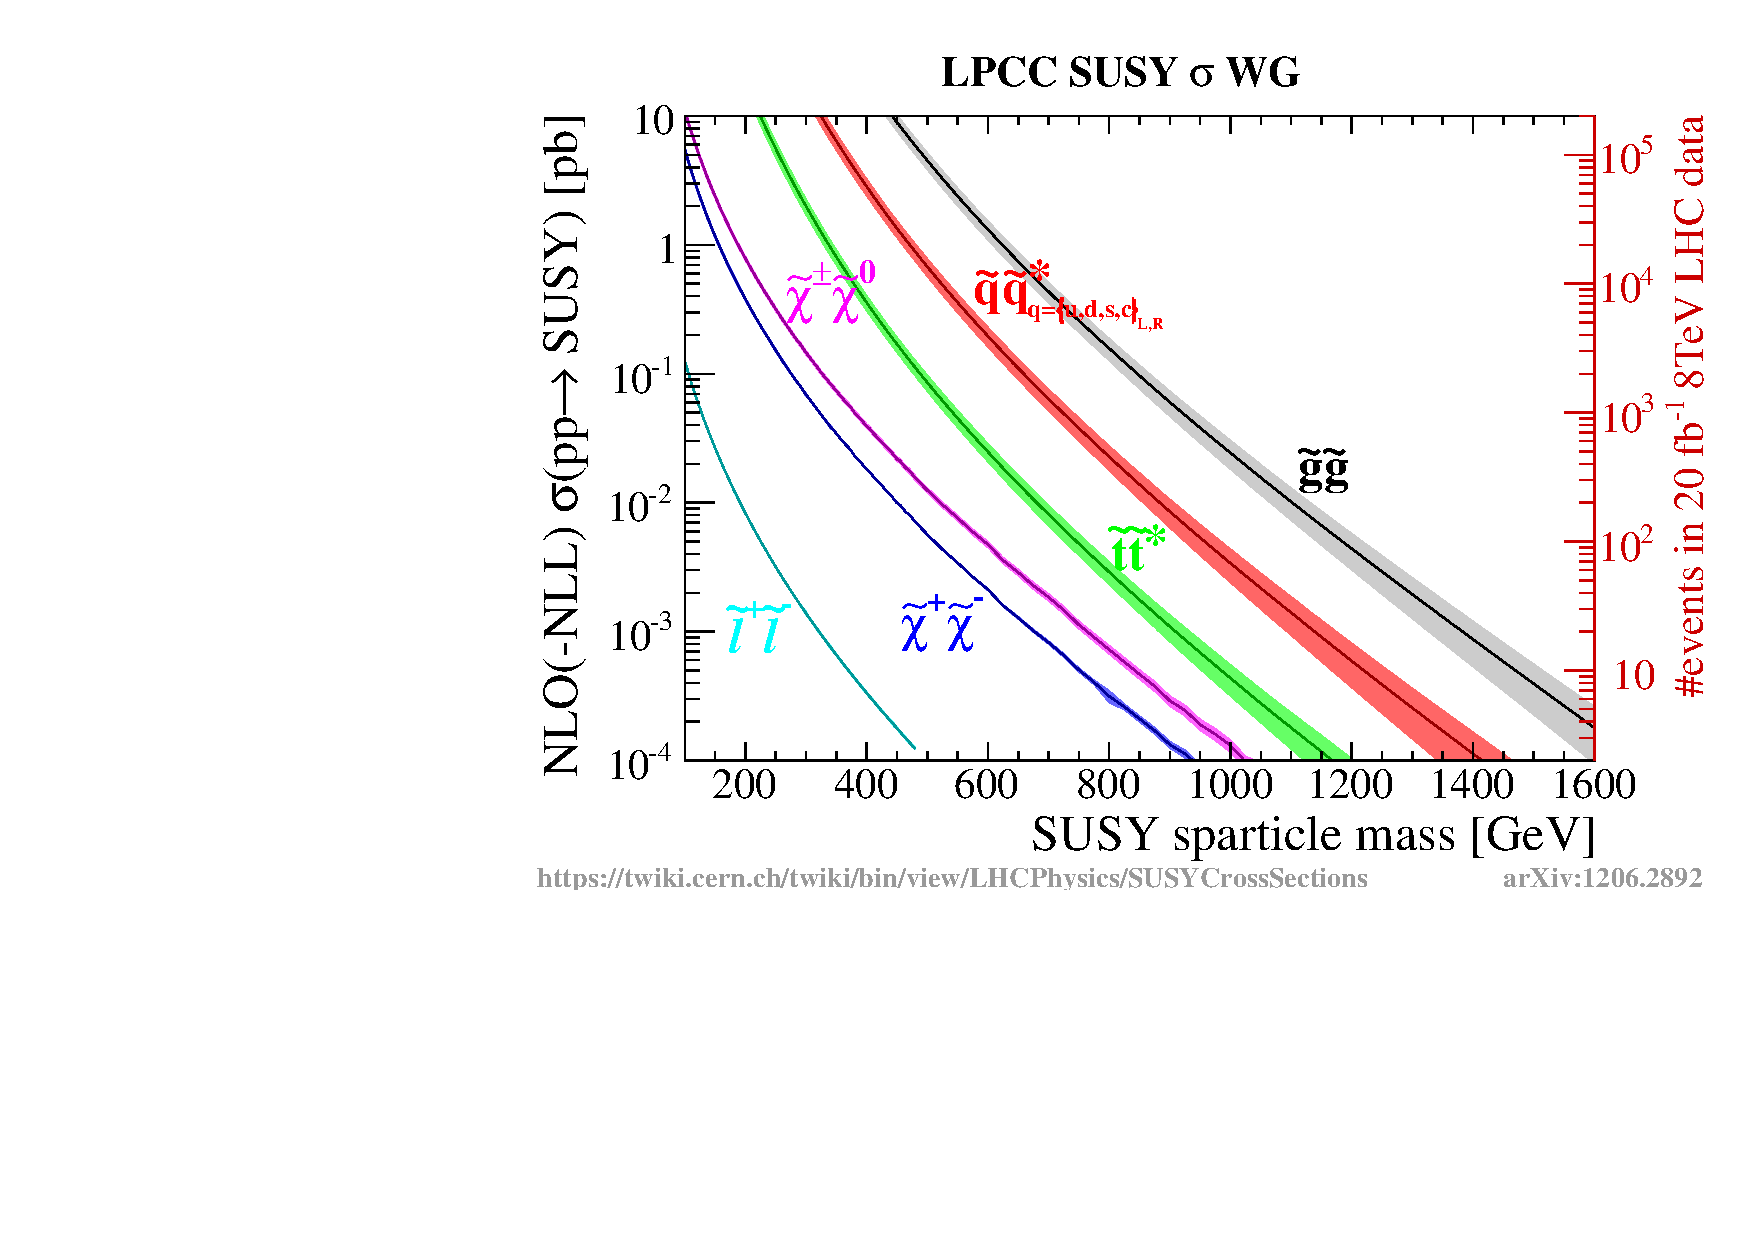
\includegraphics[width=0.65\textwidth]{figures/xsections_strong.pdf} 
  \end{tabular}
  \caption{Theory cross sections for selected SUSY processes as function of the SUSY sparticle mass. The y-axis on the right indicates the expected number of events in 20\fbinv of \pp collision data at the LHC at $\sqrt{s}=8$\tev~\cite{Kramer:2012bx}.}
  \label{fig:susy_theory_xs}
\end{figure}
It is visible that especially light-squarks and gluinos are expected at a sizable rate even for high masses above 1\tev. For instance, around 100 pairs of gluinos are expected at a mass of 1200\gev. \\
The analysis presented in this Chapter is aiming at a search for supersymmetric cascade decays arising from strongly produced light-flavour squarks or gluinos. Thus, events are selected based on the scalar sum of the jet transverse momenta (\HT), the missing transverse momentum calculated from the jet momenta (\MHT) and the number of jets (\NJets). However, the generic structure makes the analysis in principle sensitive to any new physics model that manifests in final states containing several hard jets accompanied by missing transverse energy. \\
After the description of the event selection (Sec.~\ref{sec:RA2_sel}), it is discussed how contributions from standard model processes to the selected final state are estimated. Special emphasis is put on the estimation of the QCD multijet background (Sec.~\ref{subsec:RA2_QCD}). Finally, results are presented and interpreted in various simplified supersymmetric models (Sec.~\ref{sec:RA2_results}). Parts of this Chapter are taken from~\cite{bib:AN-12-350}, having been written by the author. This analysis follows previous inclusive searches~\cite{springerlink:10.1007/JHEP08(2011)155, Chatrchyan:2012lia} and is published in~\cite{Chatrchyan:2014lfa}.    
\section{Event Selection}
\label{sec:RA2_sel}

\subsection{Data Samples and Trigger}
\label{subsec:RA2_samples_trigger}
The analysis is based on \pp collision data recorded with the CMS detector at a centre of mass energy of $\sqrt{s} = 8$\tev. This corresponds to an integrated luminosity of 19.5\fbinv for all sub-detectors fully functional. \\
The data have been collected by triggering on \HT, the scalar sum of the jet transverse momenta, and \met, the missing transverse energy. An overview of the considered runs and the integrated luminosity is shown together with the respective HLT trigger paths in Tab.~\ref{tab:RA2_trigger}. \HT and \met are calculated from particle-flow objects at trigger level with nominal thresholds of 350\gev and 100\gev, respectively. Jets considered in this calculation are reconstructed with the anti-$k_T$ algorithm and distance parameter $R = 0.5$. The labelling \textit{PFNoPU} indicates that for that particular runs also charged-hadron subtraction was applied to jets at trigger level. 
\begin{table}[!b]
\centering
\caption{Utilized signal trigger paths in individual run ranges listed together with the integrated luminosity.}
\label{tab:RA2_trigger}
 \makebox[\linewidth]{
\begin{tabular}{lccc}
\multicolumn{4}{c}{} \\
\toprule
 Trigger path & Run range & Luminosity [\fbinv] \\
\midrule
 HLT\_PFHT350\_PFMET100 & 190456 -- 196531 & 0.9 \\
 & & & \\
 HLT\_PFHT350\_PFMET100 & 190782 -- 190949 & 4.4 \\
 & & & \\
 HLT\_PFNoPUHT350\_PFMET100 & 198022 -- 198523 & 6.9 \\
 & & & \\
 HLT\_PFNoPUHT350\_PFMET100 & 198524 -- 208686 & 7.3 \\
\bottomrule
\end{tabular}}
\end{table}  
\\
In order to determine the offline values for \HT and \MHT (calculated according to the definition following in Sec.~\ref{subsec:RA2_baseline}) for which the triggers reach the plateau efficiency, the trigger efficiencies are measured with respect to a single electron trigger (HLT\_Ele27\_WP80). In principal, an orthogonal trigger is needed in order to get an unbiased estimate of the trigger efficiency. However, due to the PF-algorithm all subdetectors are used simultaneously to reconstruct the particles in an event. Hence, no independent trigger paths providing enough statistical precision are available. Consequently, only the reach of a plateau efficiency for a certain trigger path can be determined while the absolute efficiency is not accessible. The determination of the trigger plateau efficiency is performed for different jet multiplicity intervals (\NJets~$ = 3-5$, \NJets~$ = 6-7$ and \NJets~$ \ge 8$). The obtained trigger turn-on curves for the two different HLT paths are shown as function of offline \HT and \MHT for jet multiplicity \NJets~$ = 3-5$ in Fig.~\ref{fig:trig_eff_3njets5}. The respective turn-on curves for jet multiplicities $6 \leq$ \NJets $\leq 7$ and $8 \leq \NJets$ are shown in App.~\ref{fig:trig_eff_6njets7} and App.~\ref{fig:trig_eff_njets8}, respectively. For both trigger paths, the efficiency plateau is reached around offline values of \HT$ = 500$\gev and \MHT$ = 200$\gev. The integrated trigger efficiencies for these particular values in different jet multiplicity intervals are summarized with statistical uncertainties in Tab.~\ref{tab:trig_eff}. In general, they are close to 100\% with small uncertainties below 1\%. However, for the highest jet multiplicity selection of \NJets~$ \ge 8$ only few events where selected such that statistical uncertainties are few 10\% large. Though, no hints for a systematic inefficiency have been observed and the signal triggers are considered as fully efficient with an uncertainty of $2\%$ for offline values of \HT$ > 500$\gev and \MHT$ > 200$\gev independent of the jet multiplicity. \\

\begin{figure}[!t]
  \centering
  \begin{tabular}{cc}
                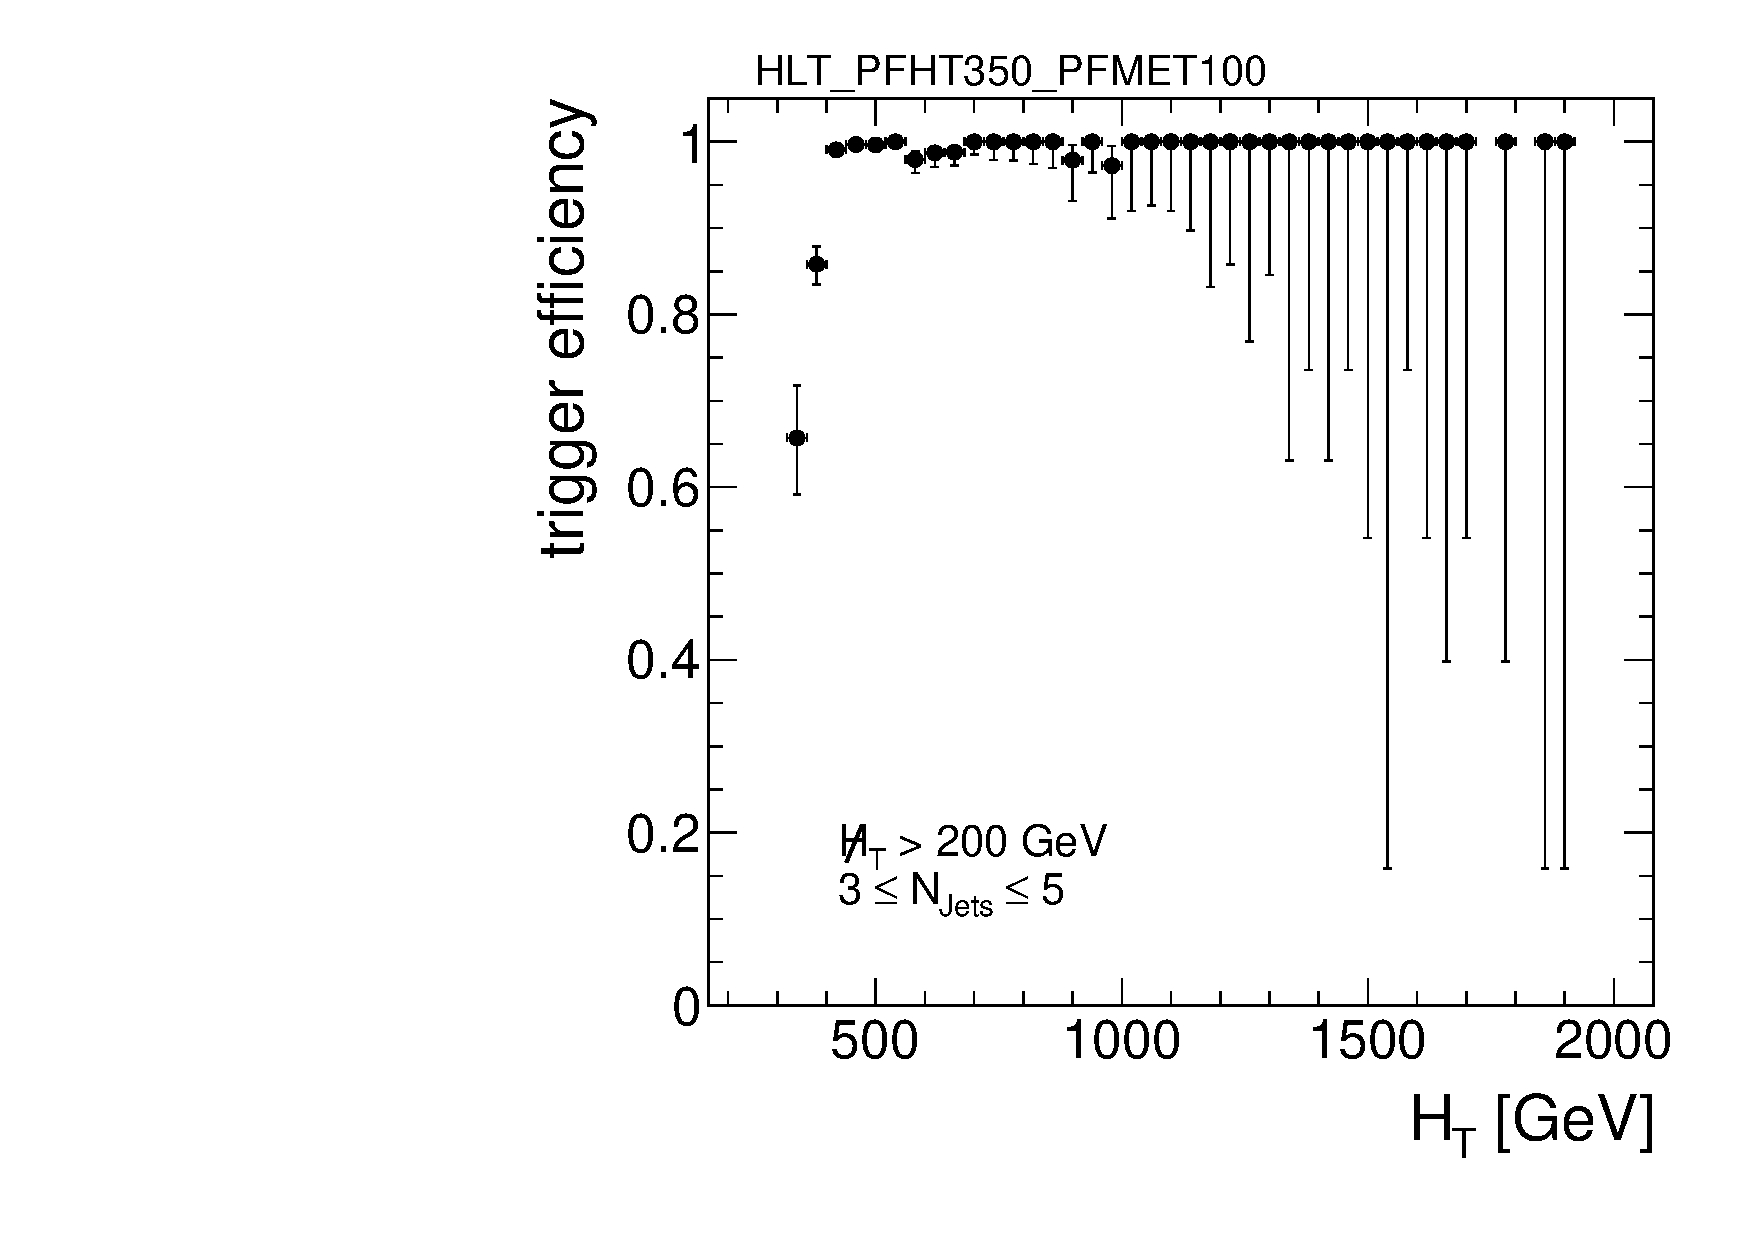
\includegraphics[width=0.49\textwidth]{figures/turn_on_HT_TagEle27WP80_ProbePFHT350PFMET100_MHT200_chs_NJets3-5.pdf} &
                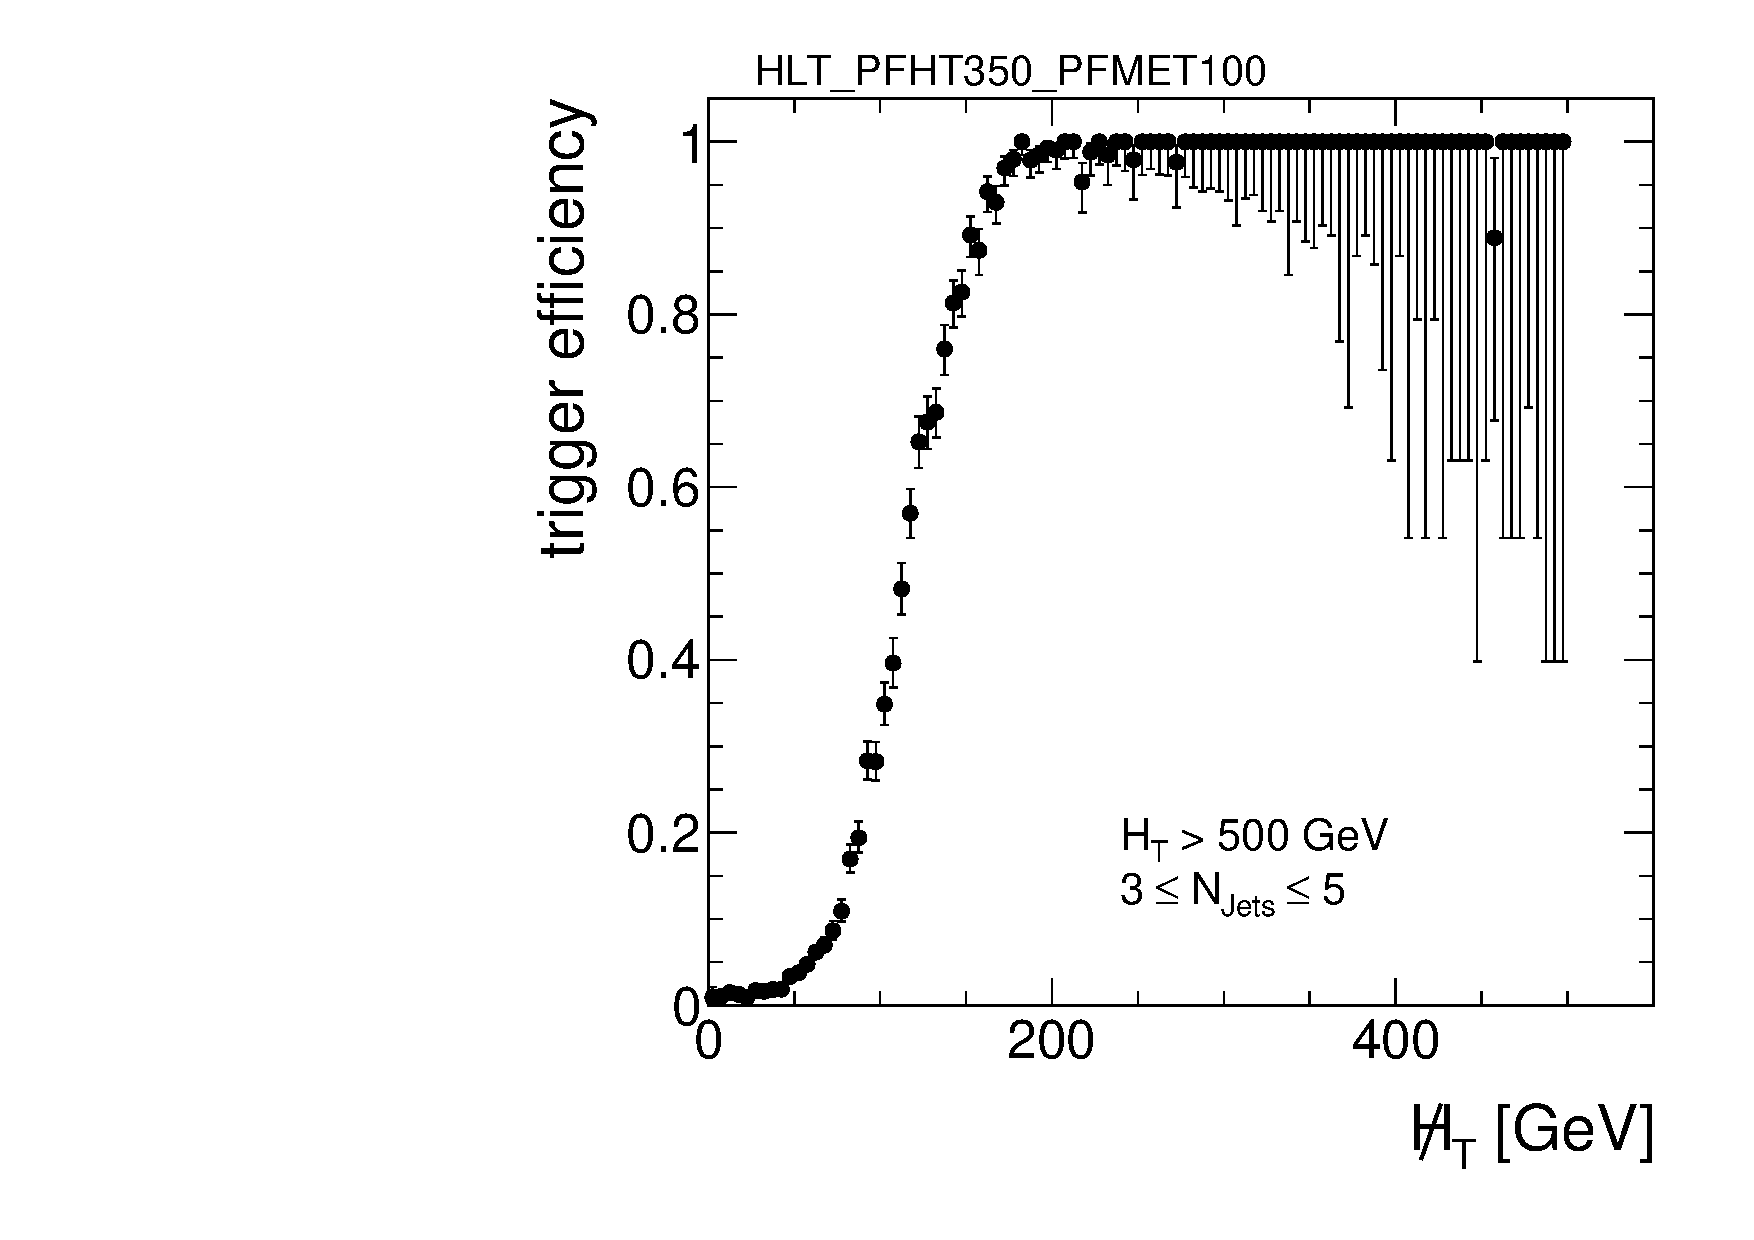
\includegraphics[width=0.49\textwidth]{figures/turn_on_MHT_TagEle27WP80_ProbePFHT350PFMET100_HT500_chs_NJets3-5.pdf} \\
                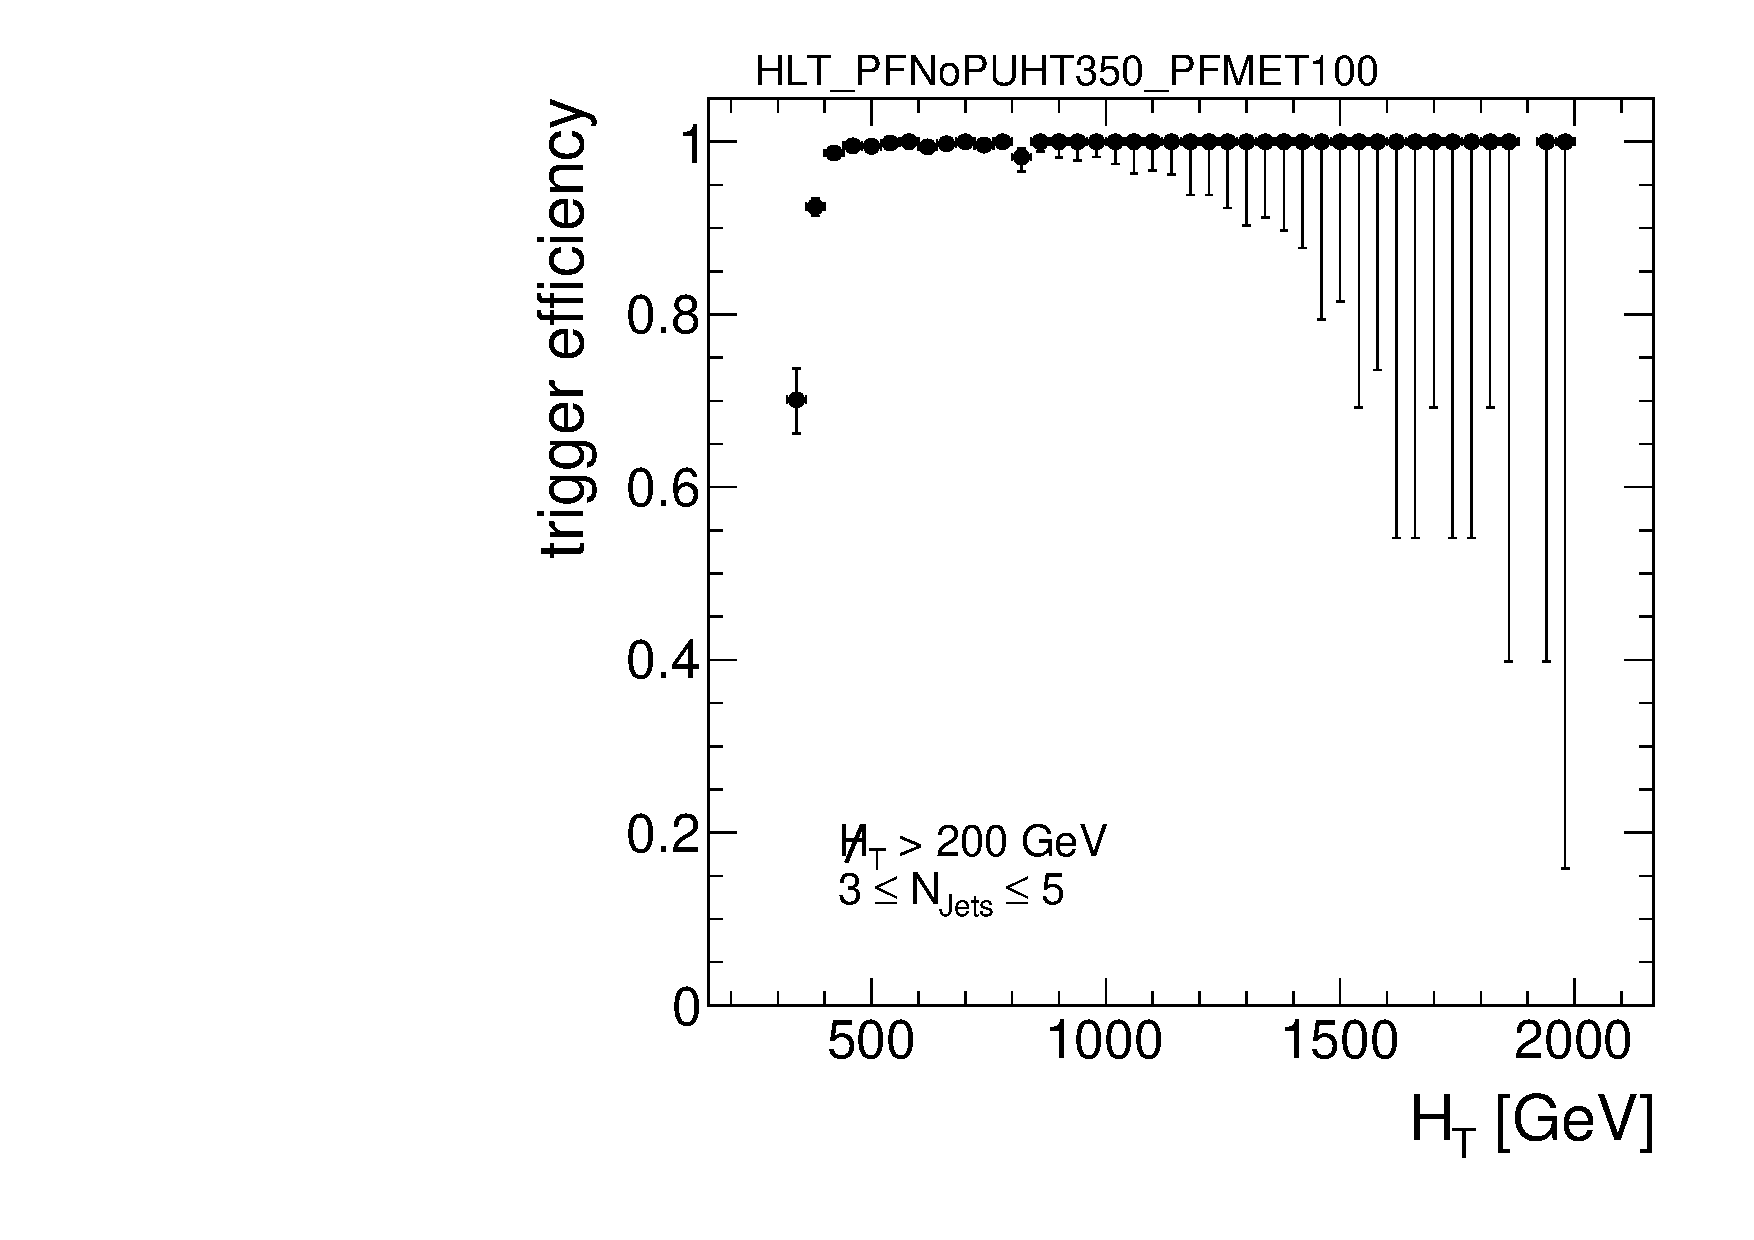
\includegraphics[width=0.49\textwidth]{figures/turn_on_HT_TagEle27WP80_ProbePFNoPUHT350PFMET100_MHT200_chs_NJets3-5.pdf} &
                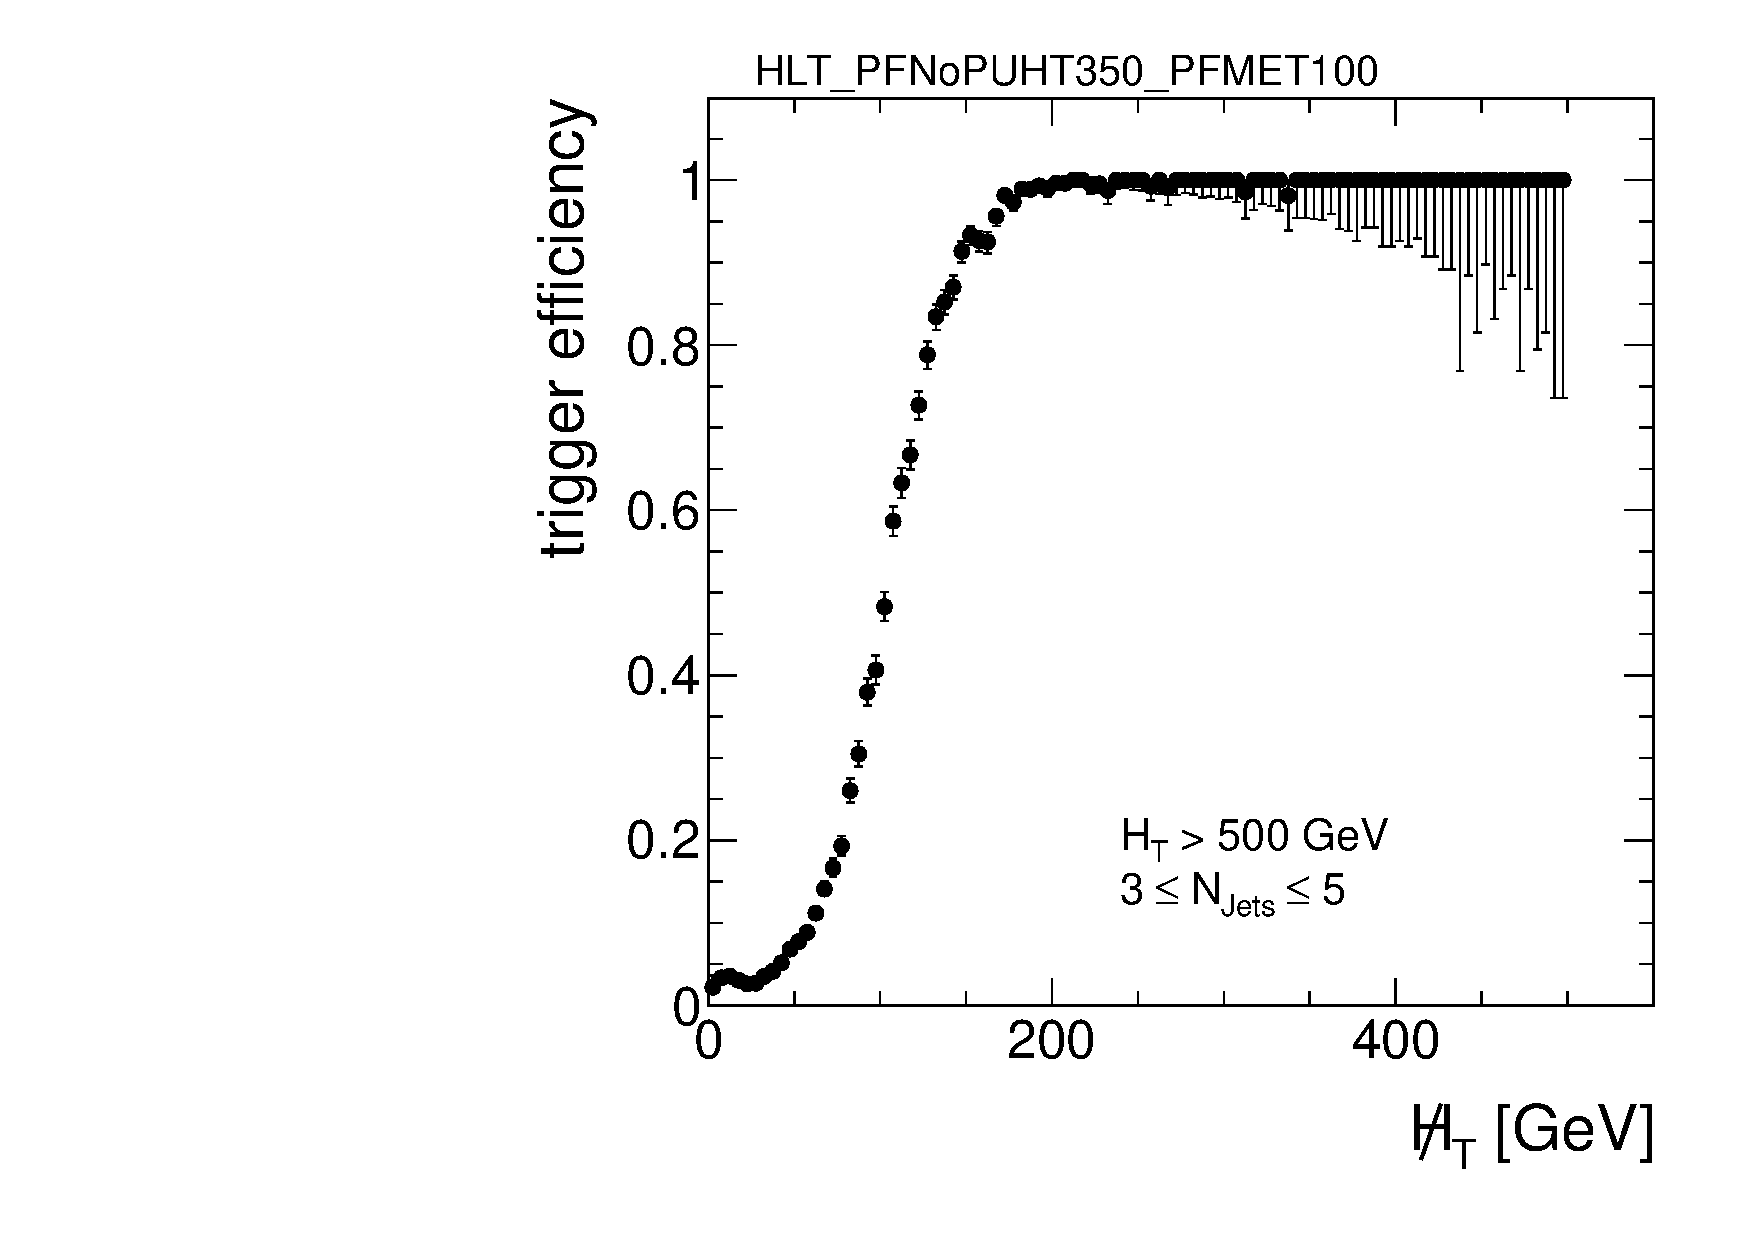
\includegraphics[width=0.49\textwidth]{figures/turn_on_MHT_TagEle27WP80_ProbePFNoPUHT350PFMET100_HT500_chs_NJets3-5.pdf} \\
  \end{tabular}
\caption{Measured trigger efficiency for paths HLT\_PFHT350\_PFMET100 (\textit{top}) and HLT\_PFNoPUHT350\_PFMET100 (\textit{bottom}) as a function of \HT (\textit{left}) and \MHT (\textit{right}) shown for $3 \leq$ \NJets $\leq 5$.} 
  \label{fig:trig_eff_3njets5}
\end{figure}

\begin{table}[!t]
  \caption{Summary of total trigger efficiencies of the signal triggers for selections of offline \HT$ > 500$\gev and \MHT$ > 200$\gev in different jet multiplicity intervals.} 
  \label{tab:trig_eff}
  \begin{center}
    \begin{tabular}{lcc}
      \toprule
      \NJets & HLT\_PFHT350\_PFMET100 &  HLT\_PFNoPUHT350\_PFMET100\\
      \midrule
      3 - 5   & $99.4 _{-0.3} ^{+0.2}$   & $99.8 _{-0.1} ^{+0.1}$\\
      6 - 7   & $99.1 _{-2.0} ^{+0.7}$   & $100.0 _{-0.6} ^{+0.0}$\\
      $\ge$ 8 & $100.0 _{-36.9} ^{+0.0}$ & $100.0 _{-10.9} ^{+0.0}$\\
      \bottomrule
    \end{tabular}
  \end{center}
\end{table}

In order to validate the basic event selection discussed in Sec.~\ref{subsec:RA2_cleaning} and~\ref{subsec:RA2_baseline} and the background estimation methods described in Sec.~\ref{subsec:RA2_QCD} and~\ref{sec:RA2_Non-QCD}, several MC simulation samples are used. The standard model processes for \ttbar, \WJets, \ZJets, $\gamma + \mathrm{{jets}}$ and QCD multijet events are generated with the MadGraph5~\cite{Alwall:2007st} generator at leading order and are interfaced with the parton-shower model in Pythia 6.4.24~\cite{Sjostrand:2006za}. They are scaled to cross-section predictions at next-to-leading order or even next-to-next-to-leading order when available~\cite{Kidonakis:2010dk, Melnikov:2006kv}. The events are processed with the full detector simulation. Furthermore, SUSY signal samples are obtained from simulation. They are generated with MadGraph5~\cite{Alwall:2007st} (with up to two additional partons), the CTEQ6L parton distribution functions~\cite{Pumplin:2002vw} and processed with the fast detector simulation. Cross sections are determined at NLO with a resummation of soft gluon emission at the accuracy of next-to-leading-log~\cite{Beenakker:1996ch, PhysRevLett.102.111802, PhysRevD.80.095004, Beenakker:2009ha, Beenakker:2011fu, Kramer:2012bx}. The cross section calculation as well as the generation of signal events for a certain type of sparticle is performed by effectively removing contributions from other sparticles by assuming their mass to be very large.

\subsection{Event Cleaning}
\label{subsec:RA2_cleaning}
The analysis presented in this Chapter realies on a precise measurement of the momentum imbalance in the event. In order to remove events with large values of fake missing momentum arising from detector noise a dedicated sequence of cleaning filters is applied: 
\begin{description}
 \item{\textbf{Primary Vertex and Beam Halo:}} Only events with at least one high-quality primary vertex are considered in the analysis. A primary vertex is classified as good, if it has more than four associated tracks and is located within 24\,cm in $z$ and 2\,cm in $xy$ direction from the nominal interaction point (\textit{good-vertex filter}). In order to reject events in which protons from the beam interact with residual gas molecules in the beam pipe, the CSC subdetector is used to identify muons moving parallel to the beam (\textit{beam-halo filter}).
 \item{\textbf{Anomalous Calorimeter Signals:}} Some events are affected by particles hitting the readout electronics or other technical instrumentation and cause anomalous signals in the ECAL or HCAL. For instance, noise in the readout system can fake artifical energy deposits at random times. Such events are identified based on timing and pulse-shape information (\textit{HBHE noise filter}). Furthermore, two $5 \times 5 $ supercrystal regions in the EE have been observed to give anomalously high energies. They are removed by imposing selections on the deposited energy in the identified supercrystals (\textit{EE bad supercrystal filter}). In order to account for transparency losses in the ECAL crystals, the system is calibrated with a dedicated laser. However, in the data some crystals are observed which receive unphysically large corrections. Events affected by this unusually large ECAL laser correction factors are rejected (\textit{ECAL laser correction filter}). The HCAL is also monitored by a dedicated laser system. Sometimes the laser fires into the collision bunch-crossing resulting in unwanted signals. These events are removed according to an event list indicating the affected events (\textit{HCAL laser filter}). The jet reconstruction utilizes information from the HO. This is used as identifier of significant leakage beyong the HCAl barrel. However, events with anomalous energy deposits in the HO have to be rejected. Thus, events in which the fraction of the momentum deposited in the HO is $> 40\%$ are removed (\textit{HO filter}).
 \item{\textbf{Dead ECAL Cells:}} Some single crystals in the ECAL are affected by malfunctioning. These single dead ECAL cells make up around $1\%$ in total and can be responsible for energy losses resulting in large values of fake-\MHT. Such events can be identified by using the trigger primitive information to determine how much energy was lost (\textit{TP filter}) or by using the surrounding energy of the masked cells (\textit{BE filter}).
 \item{\textbf{Tracking Failure:}} In some events the track reconstruction is observed to fail manifesting in large calorimeter energy deposits with lack of associated tracks. This can be caused e.g. by too many seed clusters or by collisions not taking place in the actual center of the detector. Thus, the scalar sum of track momenta associated to the good vertices divided by \HT in the event has to be larger than 10\% (\textit{tracking failure filter}) and if at least ten tracks are present in the event, good-quality tracks have to be more than 25\% (\textit{beam-scraping filter}). In addition, events with misreconstructed muon momenta in the PF algorithm (\textit{inconsistent muon filter}) or events where soft muons wrongly absorb energy from energetic HCAL towers they traverse (\textit{greedy muon filter}) are rejected. Furthermore, events with coherent noise in the strip tracker can occur. These cause several clusters distributed across the whole detector and lead to the identification of fake tracks. Such events where the track reconstruction aborted can be identified by comparing the number of pixel clusters to the number of strip clusters (\textit{many strip clusters filter}, \textit{too many strip clusters filter}, \textit{log error too many strip clusters filter}). Another failure of track reconstruction occurs sometimes when track seeds from the TOB and TEC are used. Consequently, events are rejected, if a jet with number of charged hadrons above 200 is reconstructed within $0.9 < |\eta| < 1.9$ (\textit{TOB/TEC tracking filter}).
 \item{\textbf{Noise Induced Jets:}} In order to reject events with fake jets from detector noise, events are discarded if the energy of a jet with \pt$ > 30$\gev is composed of more than 95\% from PF photon candidates or more than 90\% from PF neutral hadron energy (\textit{PBNR filter}).
\end{description}

\subsection{Baseline Selection}
\label{subsec:RA2_baseline}
The physics objects used in the analysis are reconstructed with the PF algorithm. Jets are clustered from the particle-flow objects with the anti$-k_T$ algorithm using $R = 0.5$. Furthermore, they are calibrated as discussed in Sec.~\ref{subsec:jets_calib} including residual correction factors for data. \\
The following \textit{baseline selection} criteria are used to pre-define the event sample used for the analysis.
\begin{itemize}
 \item{The number of jets (\NJets) is required to be $\ge 3$. \NJets is defined as the number of jets with $\pt > 50$\gev and $|\eta| < 2.5$. This requirement is imposed in order to select multijet events.}
 \item{The scalar sum of jet momenta (\HT) is required to be $\ge 500$\gev with 
\begin{equation*}
\HT = \sum_{\mathrm{jets}} \pt 
\end{equation*}
for all jets that have $\pt > 50$\gev and $|\eta| < 2.5$. This condition selects events with a large visible energy in the event indicating a high energy scale of the hard interaction.}   
 \item{The absolute value of the negative vectorial sum of the jet momenta (\MHT) is required to be $\ge 200$\gev with
\begin{equation*}
\MHT = |\MHTvec|= |- \sum_{\mathrm{jets}} \ptvec|
\end{equation*}
for all jets with $\pt > 30$\gev and $|\eta| < 5.0$. This selection reduces contributions from standard model processes where missing transverse momentum is expected to be small. Especially, QCD multijet background is suppressed. } 
 \item{In order to suppress events where missing transverse energy is mainly arising from jet mismeasurements, as for QCD multijet events, it is required that \MHT is not aligned with the leading three jets. Thus, events with
\begin{equation*}
\Delta \phi(\mathrm{jet}_n, \MHT) > 0.5 \;\; \mathrm{for} \;\; n = 1,2 \;\; \mathrm{and} \;\; \Delta \phi(\mathrm{jet}_3, \MHT) > 0.3
\end{equation*} 
are selected. The value of 0.5 is chosen according to the jet size parameter. However, this is reduced in case of the third jet in order to retain signal efficiency. }
 \item{Background contributions arising from \ttbar and \WJets events are reduced by rejecting events containing isolated electrons or muons with $\pt > 10$\gev. These are required to have a good quality track that can be associated with the primary interaction vertex~\cite{CMS-PAS-EGM-10-004, CMS-PAS-MUO-10-002}. The isolation is given as the scalar sum of transverse momenta of PF particles (except for the lepton itself) within a cone of width $\Delta R = 0.3$ for the electron and $\Delta R = 0.4$ for the muon, respectively. This is required to be less than 15\% of the transverse momentum of the electron and less than 20\% of the transverse momentum of the muon.}
\end{itemize}
The selection described above defines a loose validation region and provides a basis for tighter criteria. In data, 11753 events are selected after the application of the baseline selection including the event cleaning filters. A comparison of selected events in data and simulation after the basline selection is shown in Fig.~\ref{fig:ra2_baseline_mc}. Although a reasonable data and MC agreement is observed especially in the bulk of the distributions, the background estimation from simulation is not further used in the analysis, but is meant to give an impression of the relative background contributions. Since the analysis is performed in extreme tails of the \HT, \MHT and \NJets phase space with only few events and large theoretical uncertainties in the simulation, SM background contributions are estimated solely with data-based methods.

\begin{figure}[!t]
  \centering
  % \makebox[\linewidth]{
  \begin{minipage}[c]{1.\textwidth}
    \begin{center}
      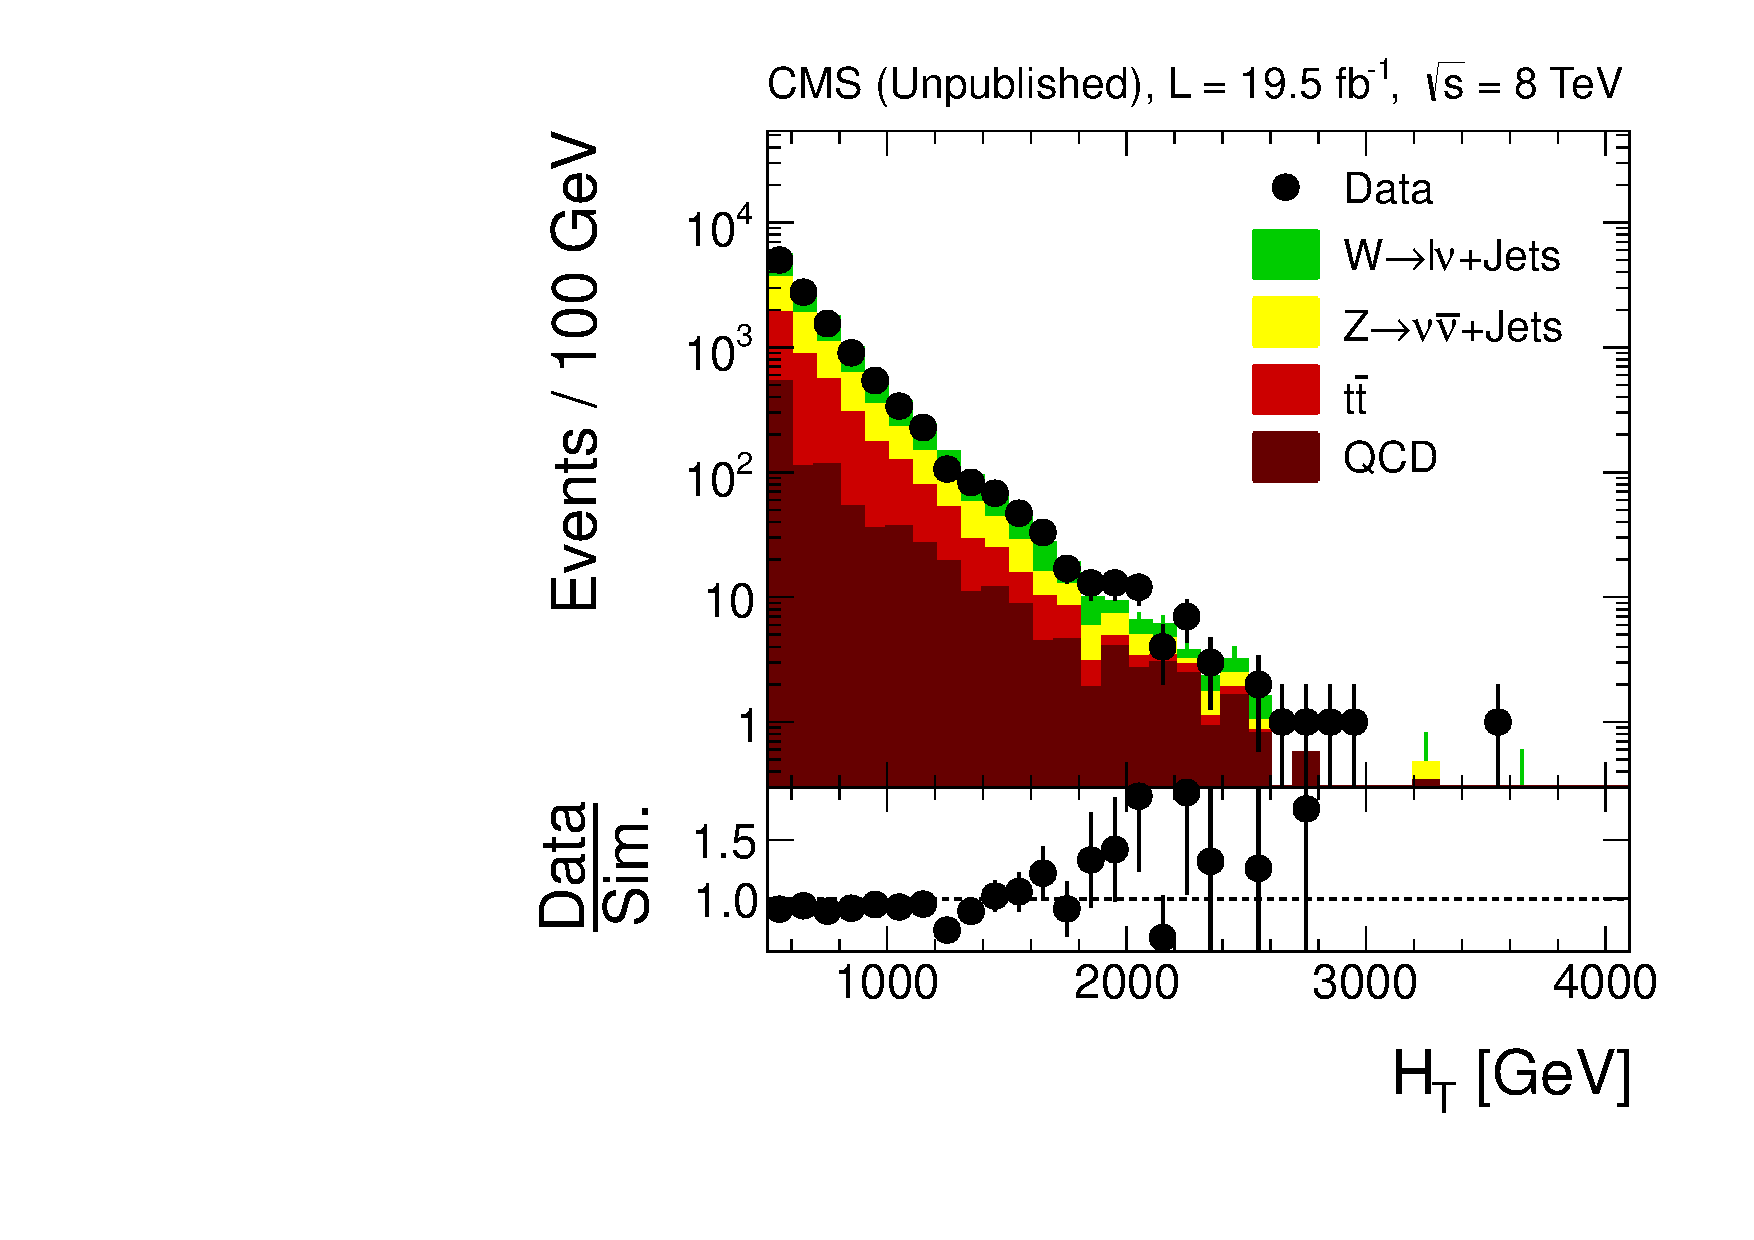
\includegraphics[width=0.49\textwidth]{figures/RA2_baseline_MC_HT.pdf}  
      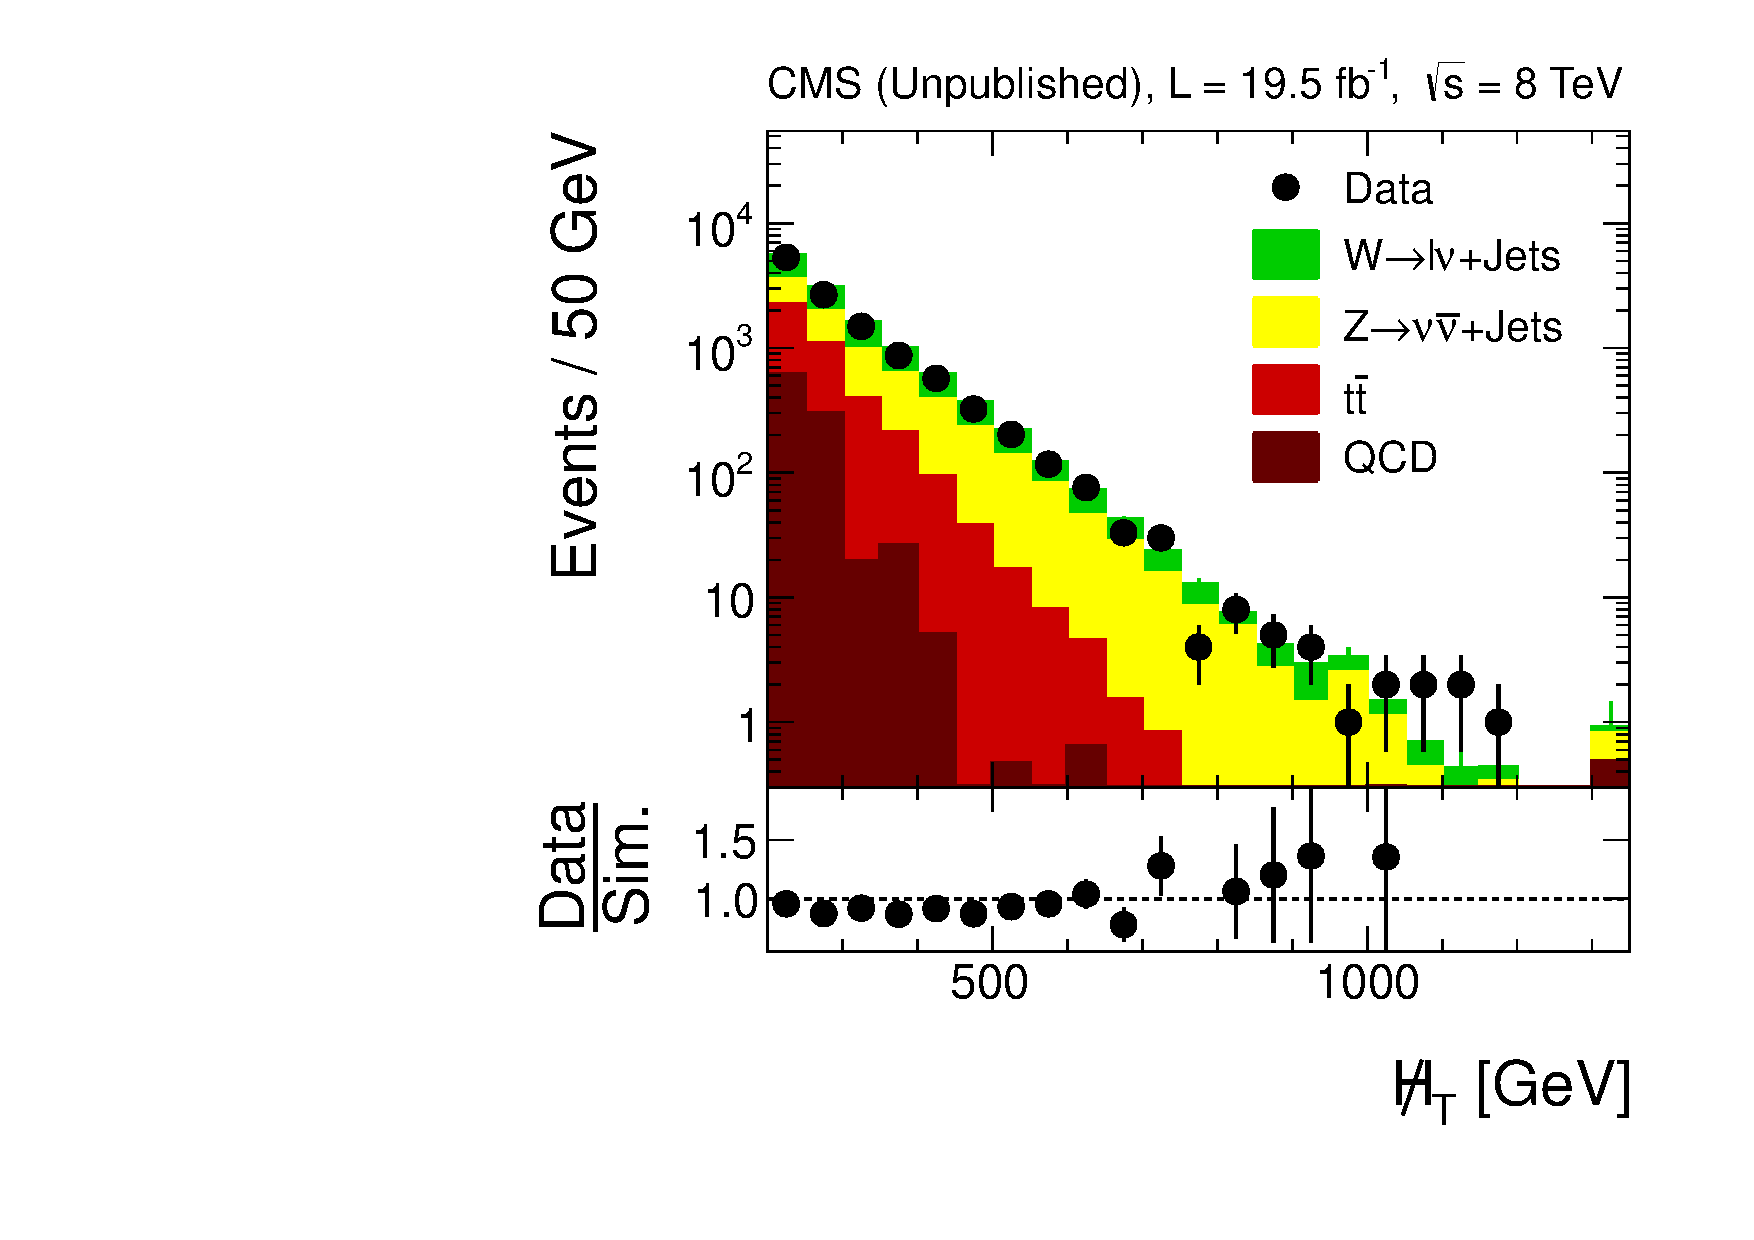
\includegraphics[width=0.49\textwidth]{figures/RA2_baseline_MC_MHT.pdf} \\
      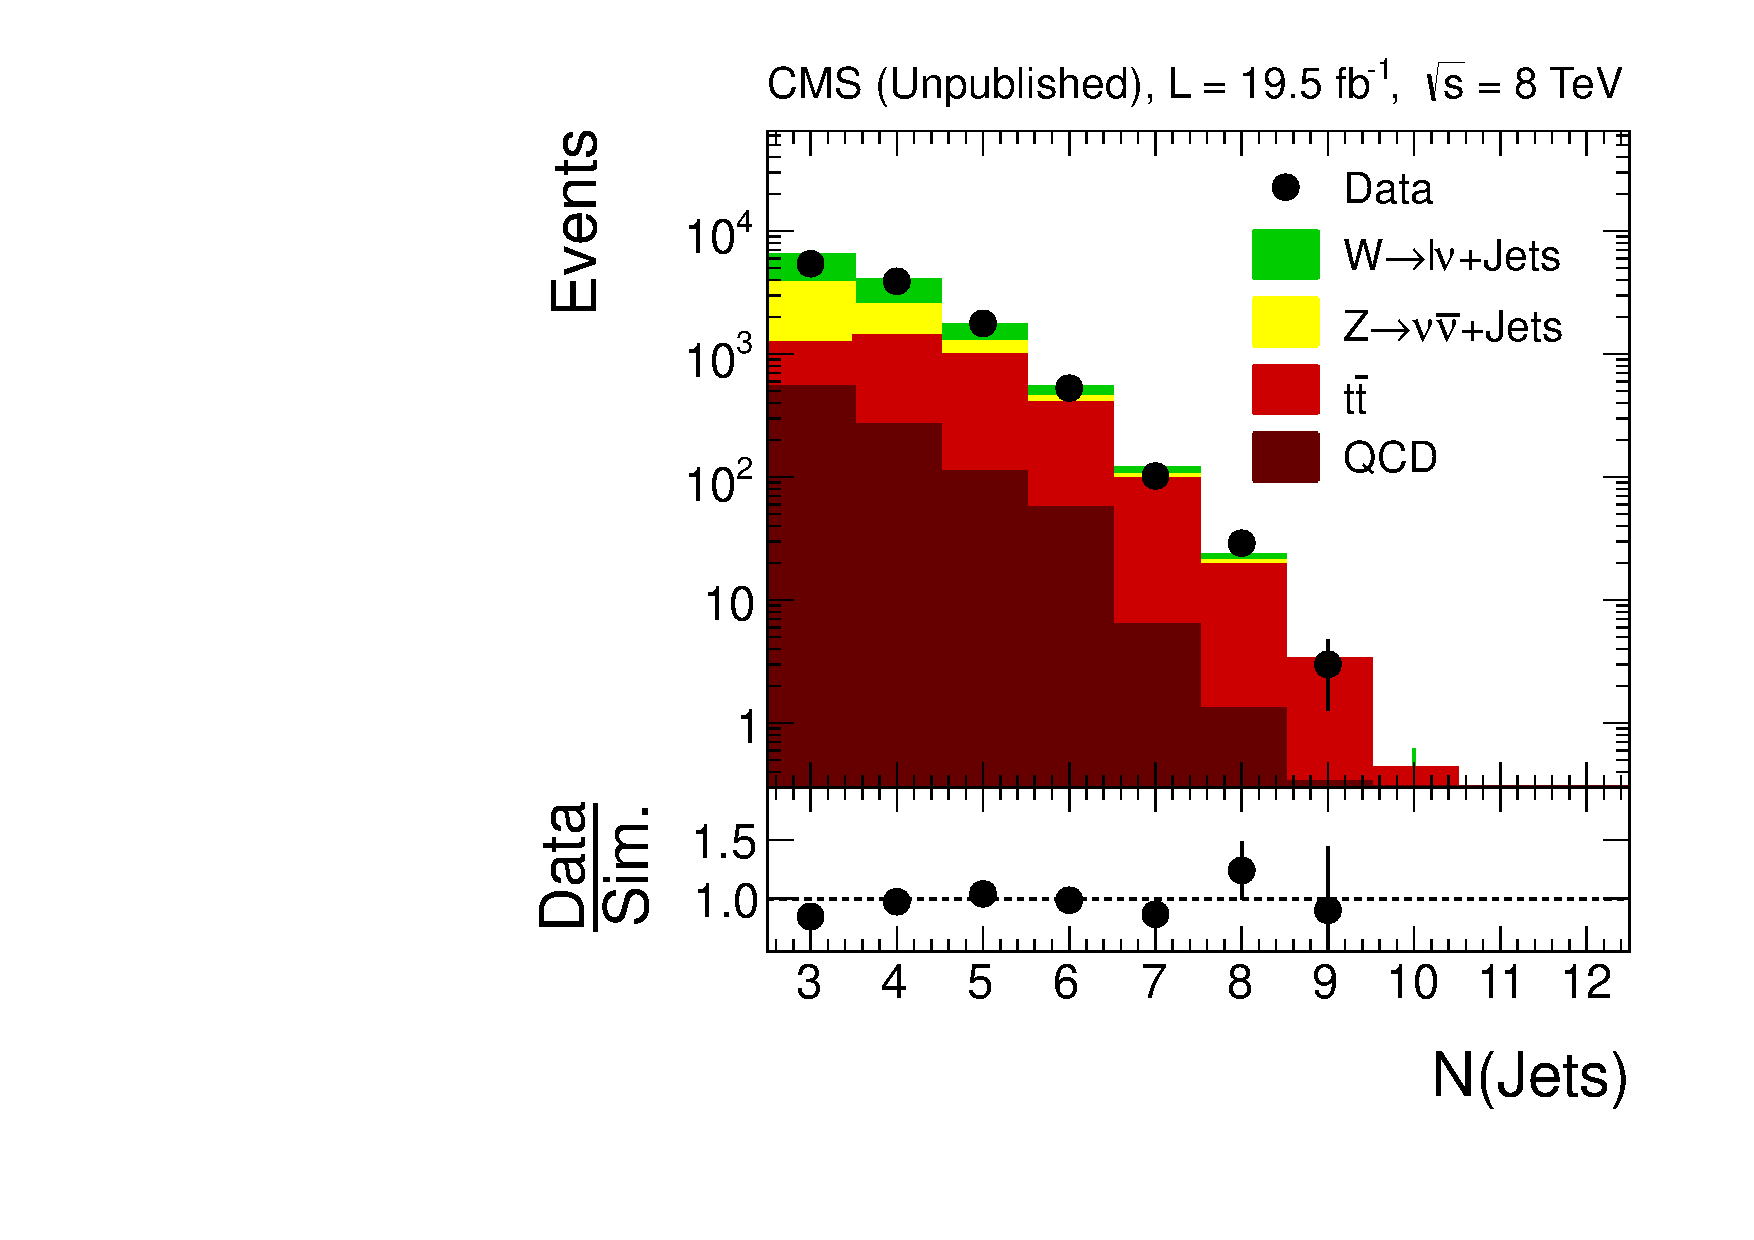
\includegraphics[width=0.49\textwidth]{figures/RA2_baseline_MC_NJets.pdf}
    \end{center}
  \end{minipage}

  \caption{Comparison of selected \HT (\textit{top left}), \MHT (\textit{top right}) and \NJets (\textit{bottom}) distributions in data (\textit{black dots}) and simulated events (\textit{shaded curve}) found from applying the event cleaning and baseline selection criteria described in Sec.~\ref{subsec:RA2_cleaning} and~\ref{subsec:RA2_baseline}. Only statistical uncertainties are shown. Taken from~\cite{Chatrchyan:2014lfa}.}
  \label{fig:ra2_baseline_mc}
\end{figure}

\subsection{Exclusive Search Regions}
\label{subsec:RA2_search_regions}
The analysis presented in this Chapter is an extension of previous inclusive searches~\cite{springerlink:10.1007/JHEP08(2011)155, Chatrchyan:2012lia}. These have been based on the requirement of at least three jets in the final state. In this analysis, the data is further subdivided into three exclusive jet multiplicity categories: $\NJets = 3 - 5, 6 - 7, \ge 8$. This enhances the sensitivity of the search towards multijet final states. These are typically the manifestations of long cascade decays from squarks and gluinos. Furthermore, it enlarges the sensitivity of the analysis to models in which gluinos often decay into top quarks. By requiring a large number of jets this analysis utilizes a complementary approach to other analyses which often use the presence of bottom-quark jets in the final state to discriminate against background~\cite{Chatrchyan:2013lya, Chatrchyan:2013wxa, CMS-PAS-SUS-13-019, CMS-PAS-SUS-14-011}. This procedure allows to keep the signal efficiency for all-hadronic final states as high as possible. In order to gain sensitivity to a variety of models, the jet categories are further classified according to \HT and \MHT. With this approach various exclusive search regions are defined. An overview of the exact definition of all 36 exclusive regions in \NJets, \HT and \MHT is given in Tab.~\ref{tab:excl_search_bins}.

\begin{table}[!h]
%\fontsize{10 pt}{1.2 em}
%\selectfont
\centering
\caption{Exclusive search regions used in the analysis binned in \HT, \MHT and \NJets.}
\begin{tabular}{lccc}
\multicolumn{4}{c}{} \\
  \toprule
   \NJets & [3-5] & [6-7] & [$\geq$8]  \\
  \midrule
             & \MHT [\gev]  & \MHT[\gev]  & \MHT[\gev]       \\
  \midrule
   500 $<$ \HT [\gev] $<$ 800   & 200-300 & 200-300 & $>$ 200 \\
                     & 300-450 & 300-450 &        \\
                     & 450-600 & $>$ 450  &        \\
                     & $>$ 600 &         &        \\
  \midrule
   800 $<$ \HT [\gev] $<$ 1000  & 200-300 & 200-300 & $>$ 200 \\
                     & 300-450 & 300-450 &        \\
                     & 450-600 & $>$ 450  &        \\
                     & $>$ 600 &         &        \\
  \midrule
   1000 $<$ \HT [\gev] $<$ 1250 & 200-300 & 200-300 & $>$ 200 \\
                     & 300-450 & 300-450 &        \\
                     & 450-600 & $>$ 450  &        \\
                     & $>$ 600 &         &        \\
  \midrule
   1250 $<$ \HT [\gev] $<$ 1500 & 200-300 & 200-300 & $>$ 200 \\
                     & 300-450 & 300-450 &        \\
                     & $>$ 450 & $>$ 450 &        \\
  \midrule
  \HT [\gev] $>$ 1500         & 200-300 & 200-300 & $>$ 200 \\
                     & $>$ 300  & $>$ 300  &        \\
  \bottomrule
\end{tabular}
\label{tab:excl_search_bins}
\end{table}    

\section{Estimation of Non-QCD Backgrounds}
\label{sec:RA2_Non-QCD}
As discussed in Sec.~\ref{subsec:susy_collider}, events from the SM processes \ZInvJets, \WJets or semi-leptonic \ttbar (where either the lepton is lost or a hadronically decaying $\tau$ lepton) and mismeasured QCD multijet events constitute important background contributions to all-hadronic final states. Dedicated data-based methods are employed to estimate their size in the selected data. In this Section those methods are described starting with a short review of the estimation of non-QCD backgrounds (Sec.~\ref{subsec:RA2_Zinv}, Sec.~\ref{subsec:RA2_tauhad} and Sec.~\ref{subsec:RA2_lostlepton}) followed by a detailled discussion of the QCD background estimation (Sec.~\ref{subsec:RA2_QCD}). 

\subsection{Invisible Z Background}
\label{subsec:RA2_Zinv}
\begin{figure}[!t]
  \centering
\makebox[\linewidth]{
  \begin{tabular}{cc}
                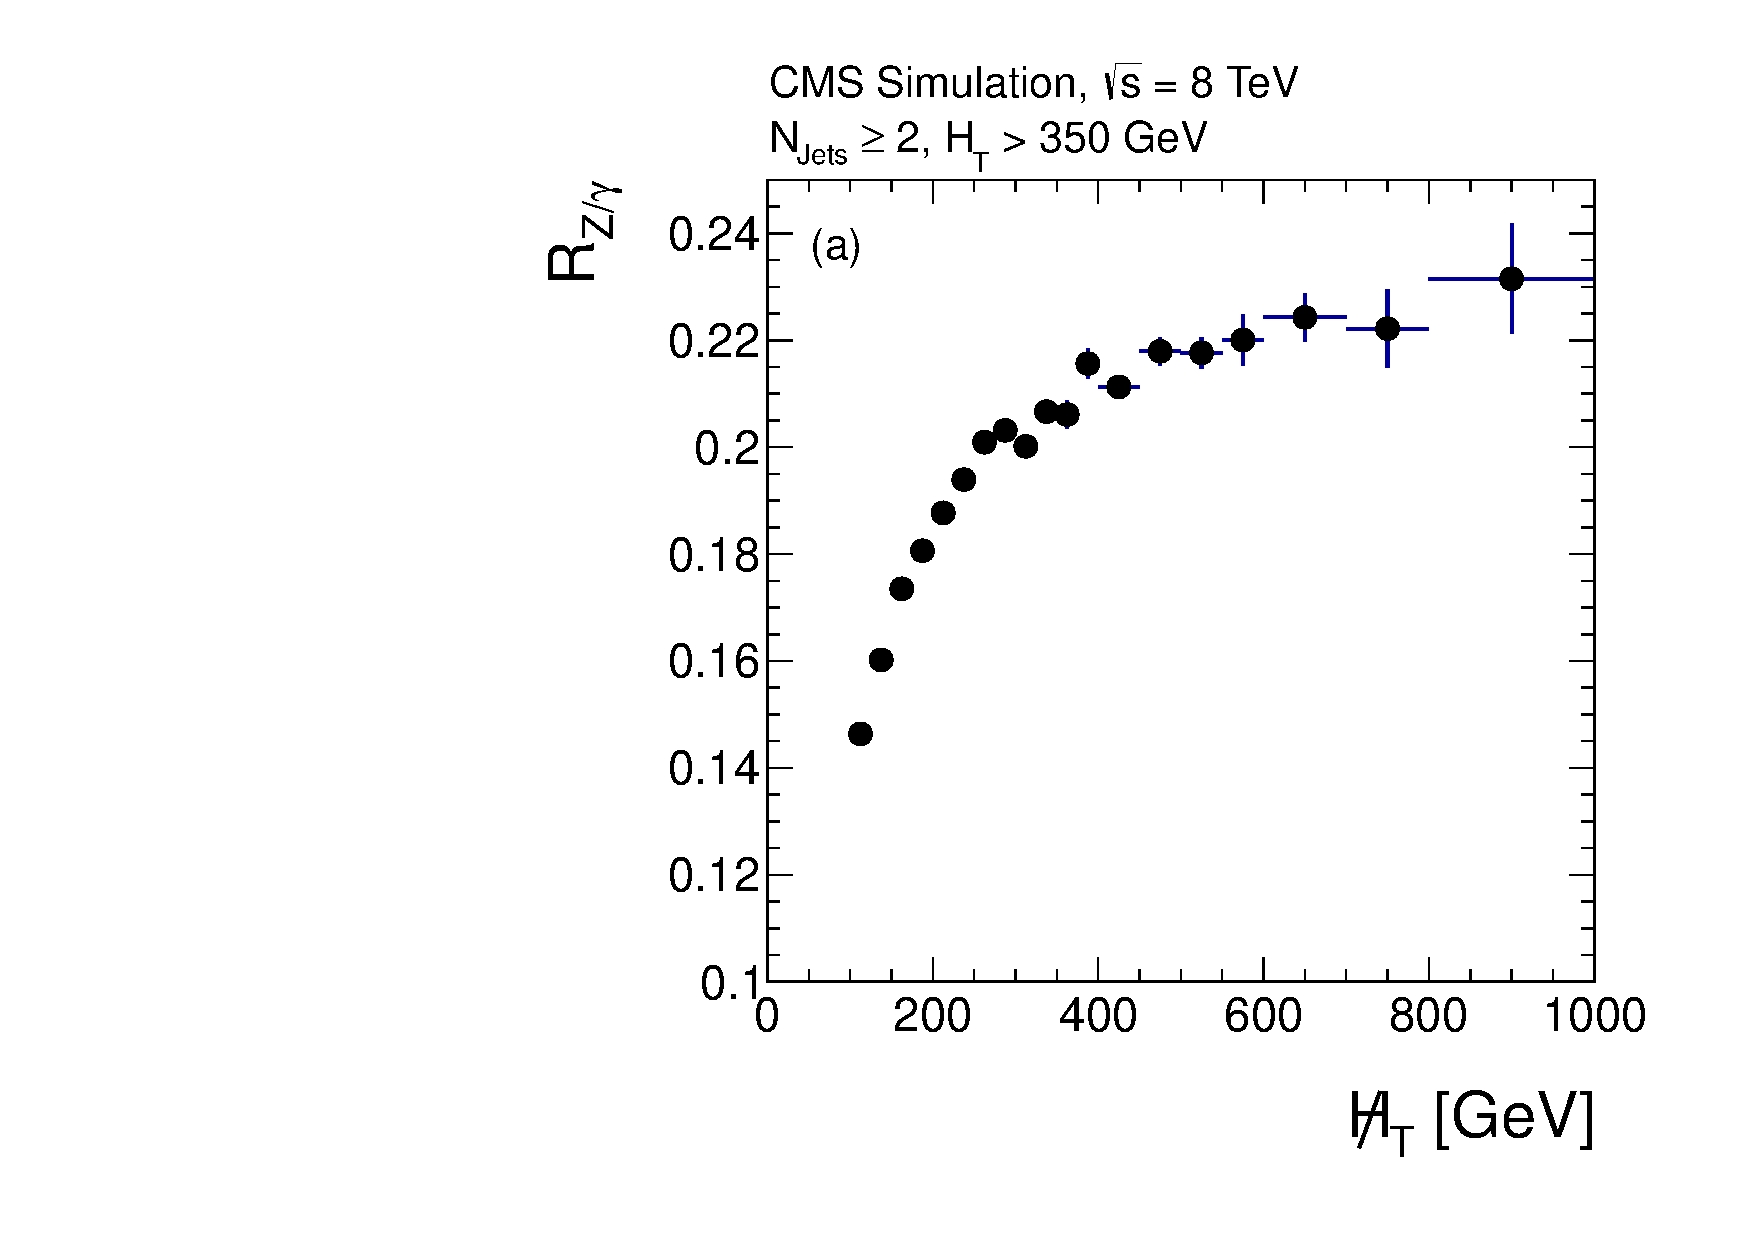
\includegraphics[width=0.49\textwidth]{figures/RA2_Zinv1.pdf} & 
                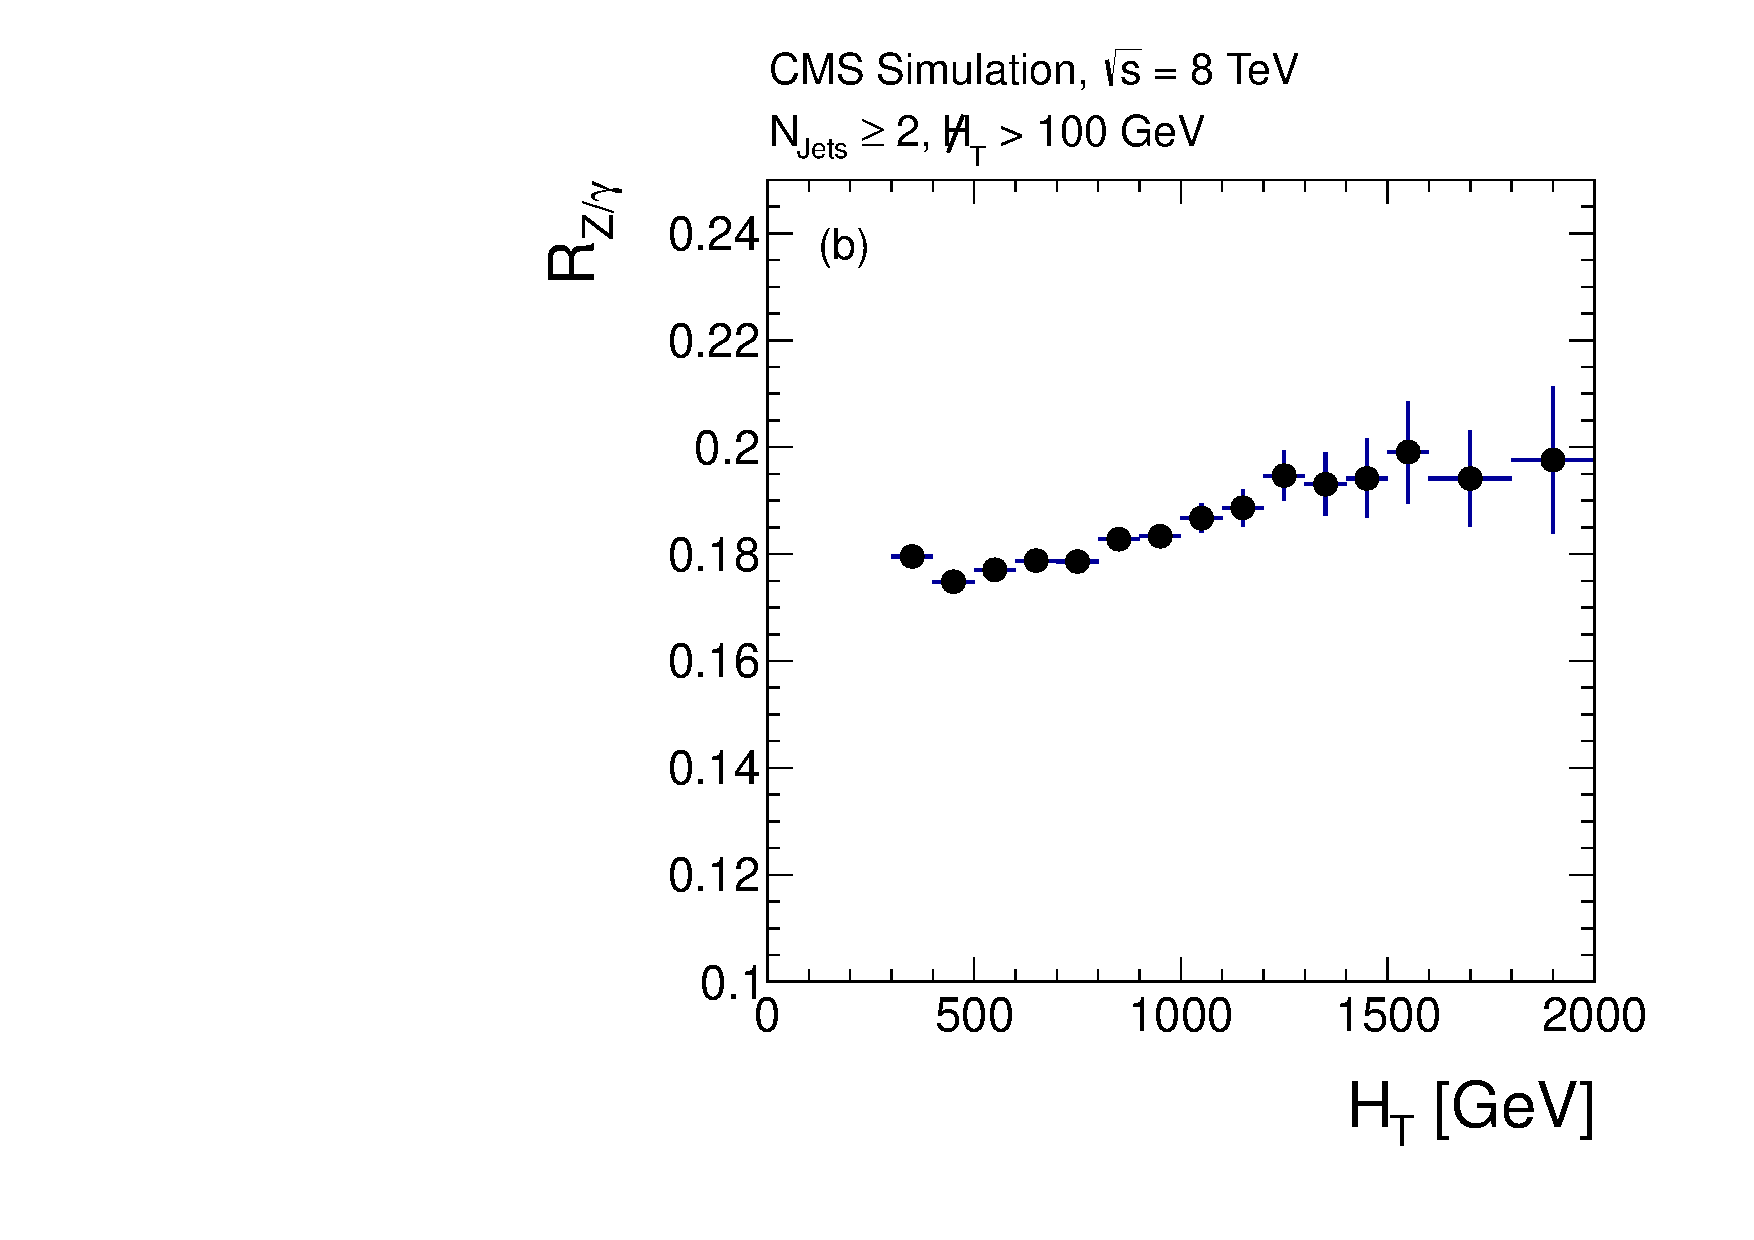
\includegraphics[width=0.49\textwidth]{figures/RA2_Zinv2.pdf} \\
                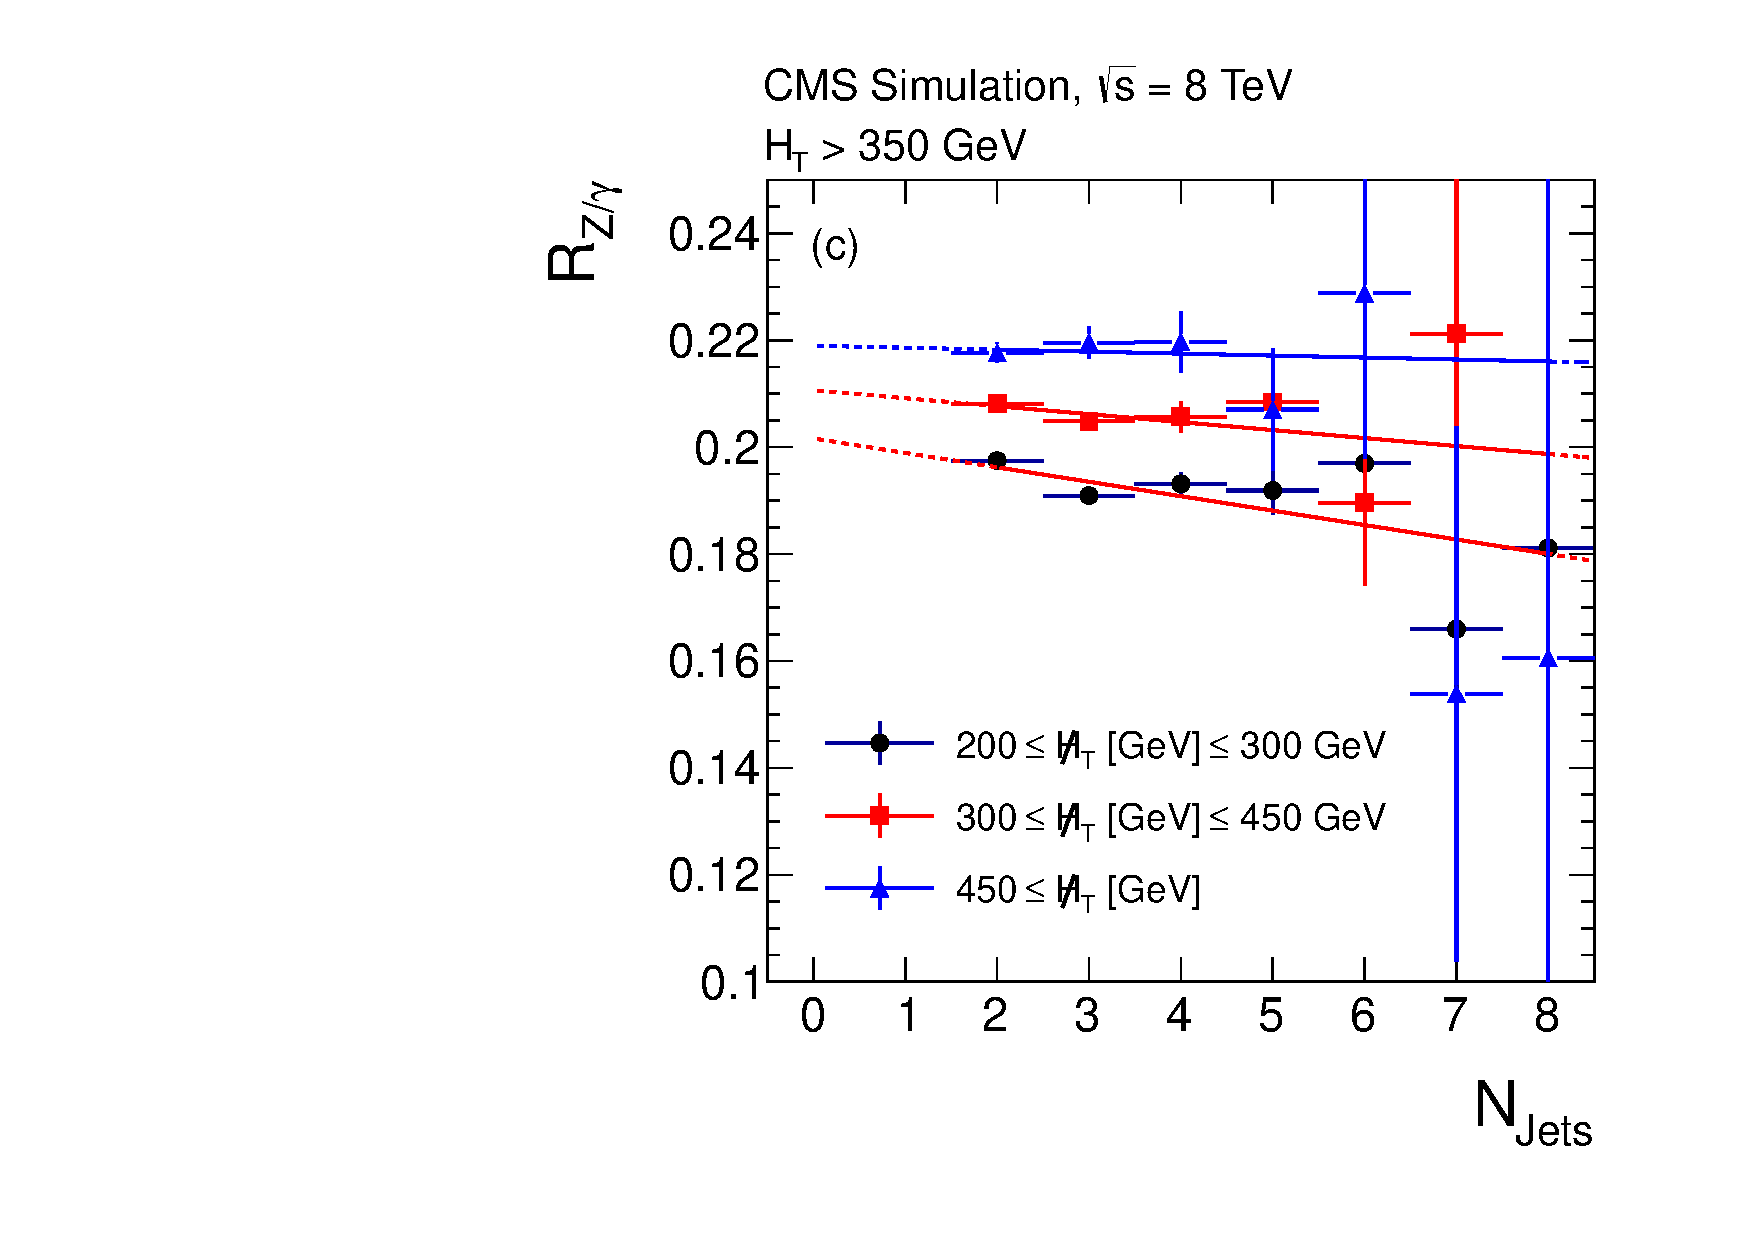
\includegraphics[width=0.49\textwidth]{figures/RA2_Zinv3.pdf} &
                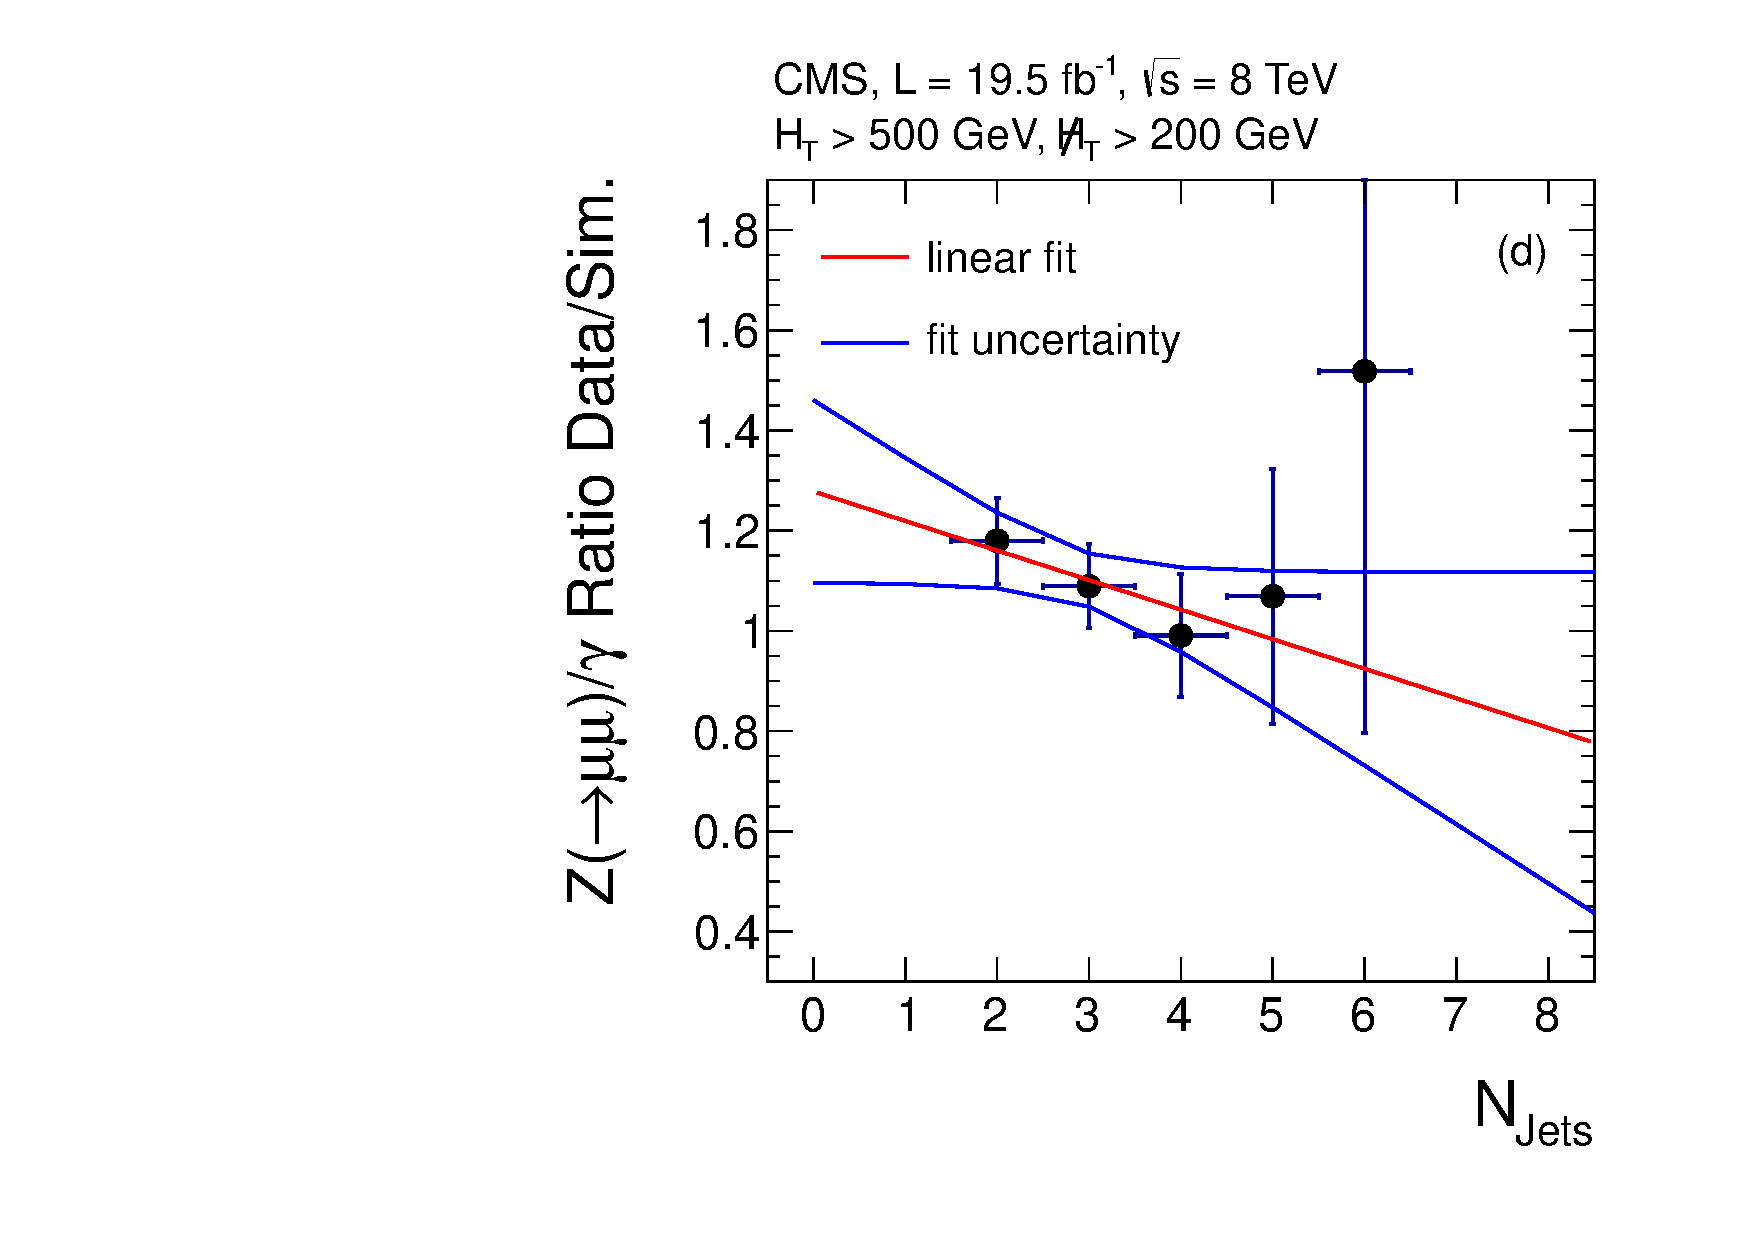
\includegraphics[width=0.49\textwidth]{figures/RA2_Zinv4.pdf}
  \end{tabular}}
  \caption{The simulated ratio $R_{Z/\gamma}$ as a function of (a) \MHT, (b) \HT, (c) \NJets, where the values for three \MHT selections are shown with linear fits, and (d) the double ratio of $R_{Z(\mu+\mu-)/\gamma}$, using events from data to those from simulation; the linear fit and its uncertainty band are overlaid. Taken from~\cite{Chatrchyan:2014lfa}.}
  \label{fig:ra2_zinv}
\end{figure}
The irreducible background contributions arising from \ZInvJets events are estimated using \photonJets events. This is a well suited method as for high transverse momenta of the vector boson the event kinematics are basically the same and the cross sections differ only according to the different couplings~\cite{Ask:2011xf, Bern:2012vx}. \\
The \photonJets sample is collected by triggering on a $\photon$ candidate and large values of \HT. Photon candidates are selected if they satisfy \pt$ > 100$\gev and $|\eta| < 1.44$ or $1.566 < |\eta| < 2.5$. Furthermore, they have to have a shower profile consistent with that of a prompt photon produced directly in the hard interaction. In order to distinguish photons from misidentified electrons they must not have an associated track in the pixel detector. In addition, photon candidates are required to be isolated meaning that in a cone of $\Delta R = 0.3$ the summed transverse momenta of PF candidates around the momentum direction of the photon candidate are not allowed to exceed a certain value. The number of selected \photonJets events is corrected for photon acceptance, reconstruction and isolation efficiency. Furthermore, the purity of the \photonJets sample which is the fraction of selected photon candidates emerging from direct production has to be taken into account. The number of background photons caused \eg by misidentified jet fragments, is estimated by exploiting the difference between the shower profile of prompt and background photons. The average purity of the \photonJets sample is measured to be 93\%.\\
Subsequently, the number of \ZInvJets events in data $N_{\ZInvJets}^{\text{data}} (\HT, \MHT, \NJets)$ using the number of selected \photonJets events $N_{\photonJets}^{\text{data}} (\HT,\MHT,\NJets)$ is obtained according to
\begin{equation*}
N_{\ZInvJets}^{\text{data}} (\HT, \MHT, \NJets) = R^{\text{MC}}_{Z(\nu\bar{\nu})/\gamma} (\HT,\MHT,\NJets)
                                                        \times 
                                                       \frac{R_{Z(\mu\mu)/\gamma}^{\text{data}}}{R_{Z(\mu\mu)/\gamma}^{\text{MC}}}
                                                        \times 
                                                       N_{\photonJets}^{\text{data}} (\HT,\MHT,\NJets)
\label{eqn:photoncorr}
\end{equation*}
with the ratio relating the production cross section of \ZInvJets and \photonJets events $R^{\text{MC}}_{Z(\nu\bar{\nu})/\gamma} (\HT,\MHT,\NJets)$ determined in simulation and the double ratio $\frac{R_{Z(\mu\mu)/\gamma}^{\text{data}}}{R_{Z(\mu\mu)/\gamma}^{\text{MC}}}$ selected in data and MC to consider the theoretical uncertainty and correct $R_{Z/\gamma}$ for a given jet multiplicity. The missing momentum in the event is emulated by ignoring the momentum of the photon candidate in the calculation of \MHT. \\
The behaviour of $R_{Z/\gamma}$ is examined in simulated events as function of \MHT, \HT and \NJets. The obtained distributions are shown in Fig.~\ref{fig:ra2_zinv}\,(a) -- (c). While a strong dependence on \MHT for small values ($\lesssim 500$\gev) is observed, the variation as function of \HT amounts to only $(12 \pm 5)\%$ in the relevant range for this analysis of $\HT = 500 - 1500$\gev. The ratio as function of the jet multiplicity is determined for different \MHT ranges of $\MHT = 200 - 300$\gev, $\MHT = 300 - 450$\gev and $\MHT > 450$\gev. The behaviour in each of these \MHT ranges is described by a linear function also displayed in Fig.~\ref{eqn:photoncorr}\,(c). It is found that the ratio decreases slightly with increasing jet multiplicity which is consistent with findings from theory~\cite{Bern:2012vx, Bern:2011pa}. \\
In order to take the theoretical uncertainty on $R_{Z/\gamma}$ into account this phenomenological ratio is also determined for $Z_{\mu^+\mu^-}$ events in data and simulation, respectively. The double ratio of $R_{Z(\mu\mu)/\gamma}^{\text{data}}$ to $R_{Z(\mu\mu)/\gamma}^{\text{MC}}$ is derived as function of the jet multiplicity and shown in Fig.~\ref{eqn:photoncorr}\,(d). It is fitted with a linear function and the deviation from unity is considered as correction for the $R_{Z/\gamma}$ ratio in each jet multiplicity selection. \\
The main sources of uncertainty for the prediction of \ZInvJets events arise from the fit uncertainty to the double ratio which is at the order of 20\%, 25\% and 45\% for the different jet multiplicity intervals, the differences between data and simulation regarding the photon identification and isolation as well as the subtraction of background photons from QCD multijet events.

\subsection{Hadronic-tau Background}
\label{subsec:RA2_tauhad}
\begin{figure}[!t]
  \centering

  \begin{minipage}[c]{1.\textwidth}
    \begin{center}
      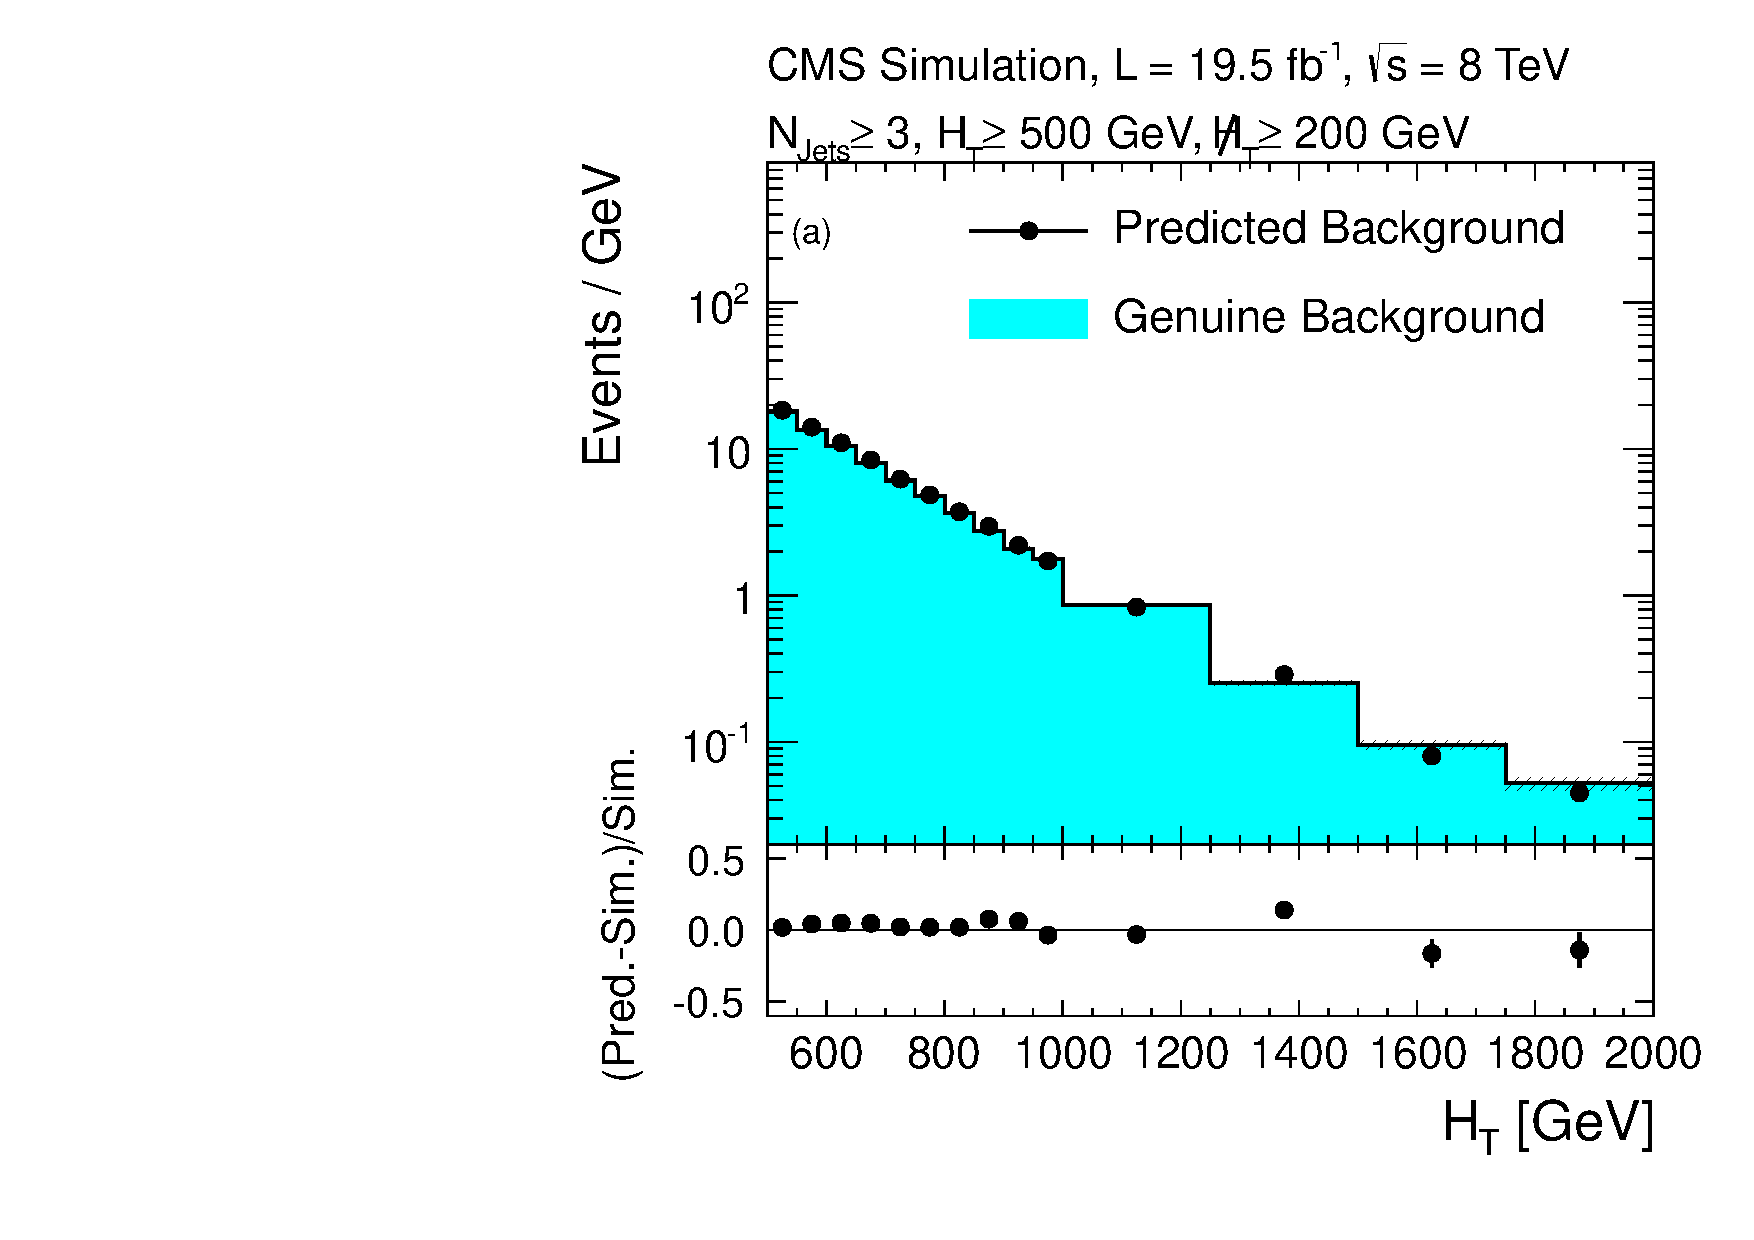
\includegraphics[width=0.49\textwidth]{figures/RA2_TauHad1.pdf}% \hspace {1.5 pt} 
      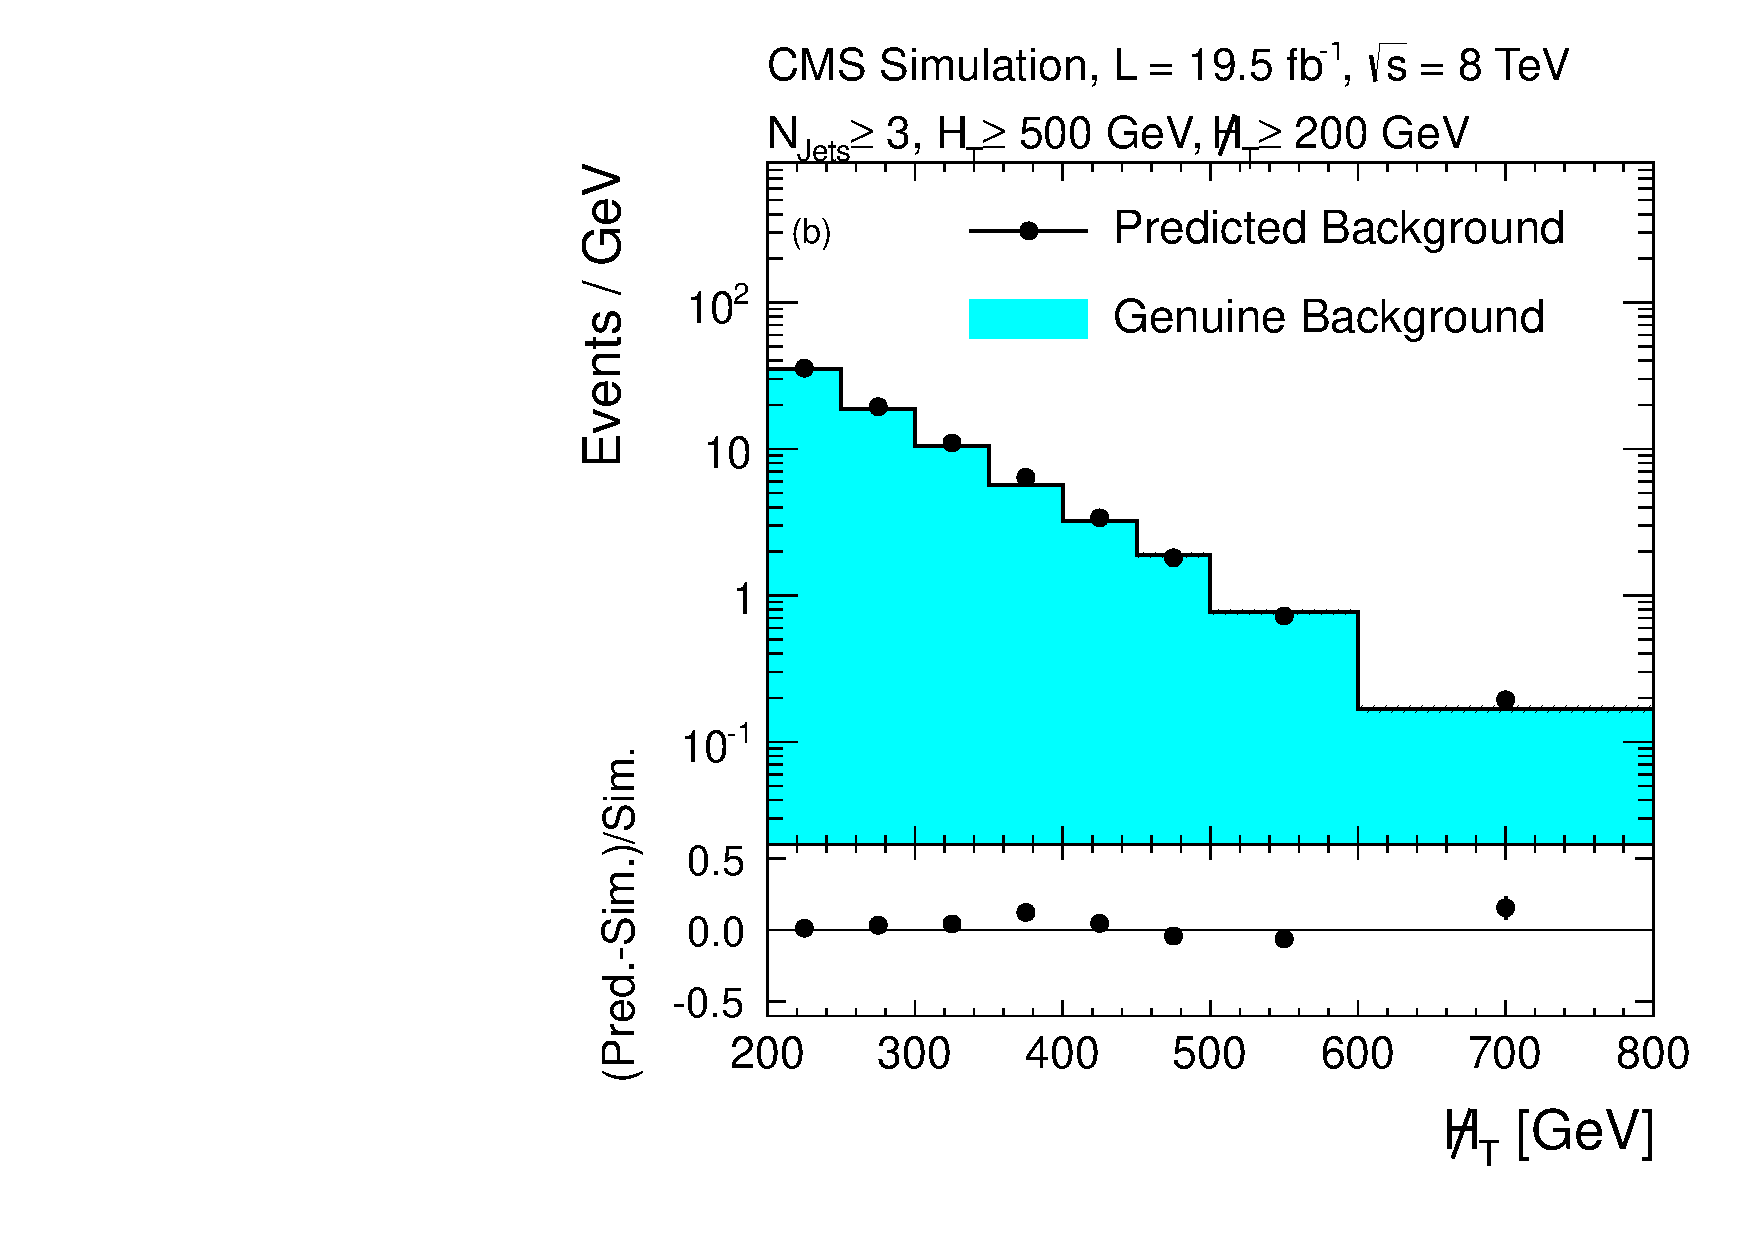
\includegraphics[width=0.49\textwidth]{figures/RA2_TauHad2.pdf}\\ 
      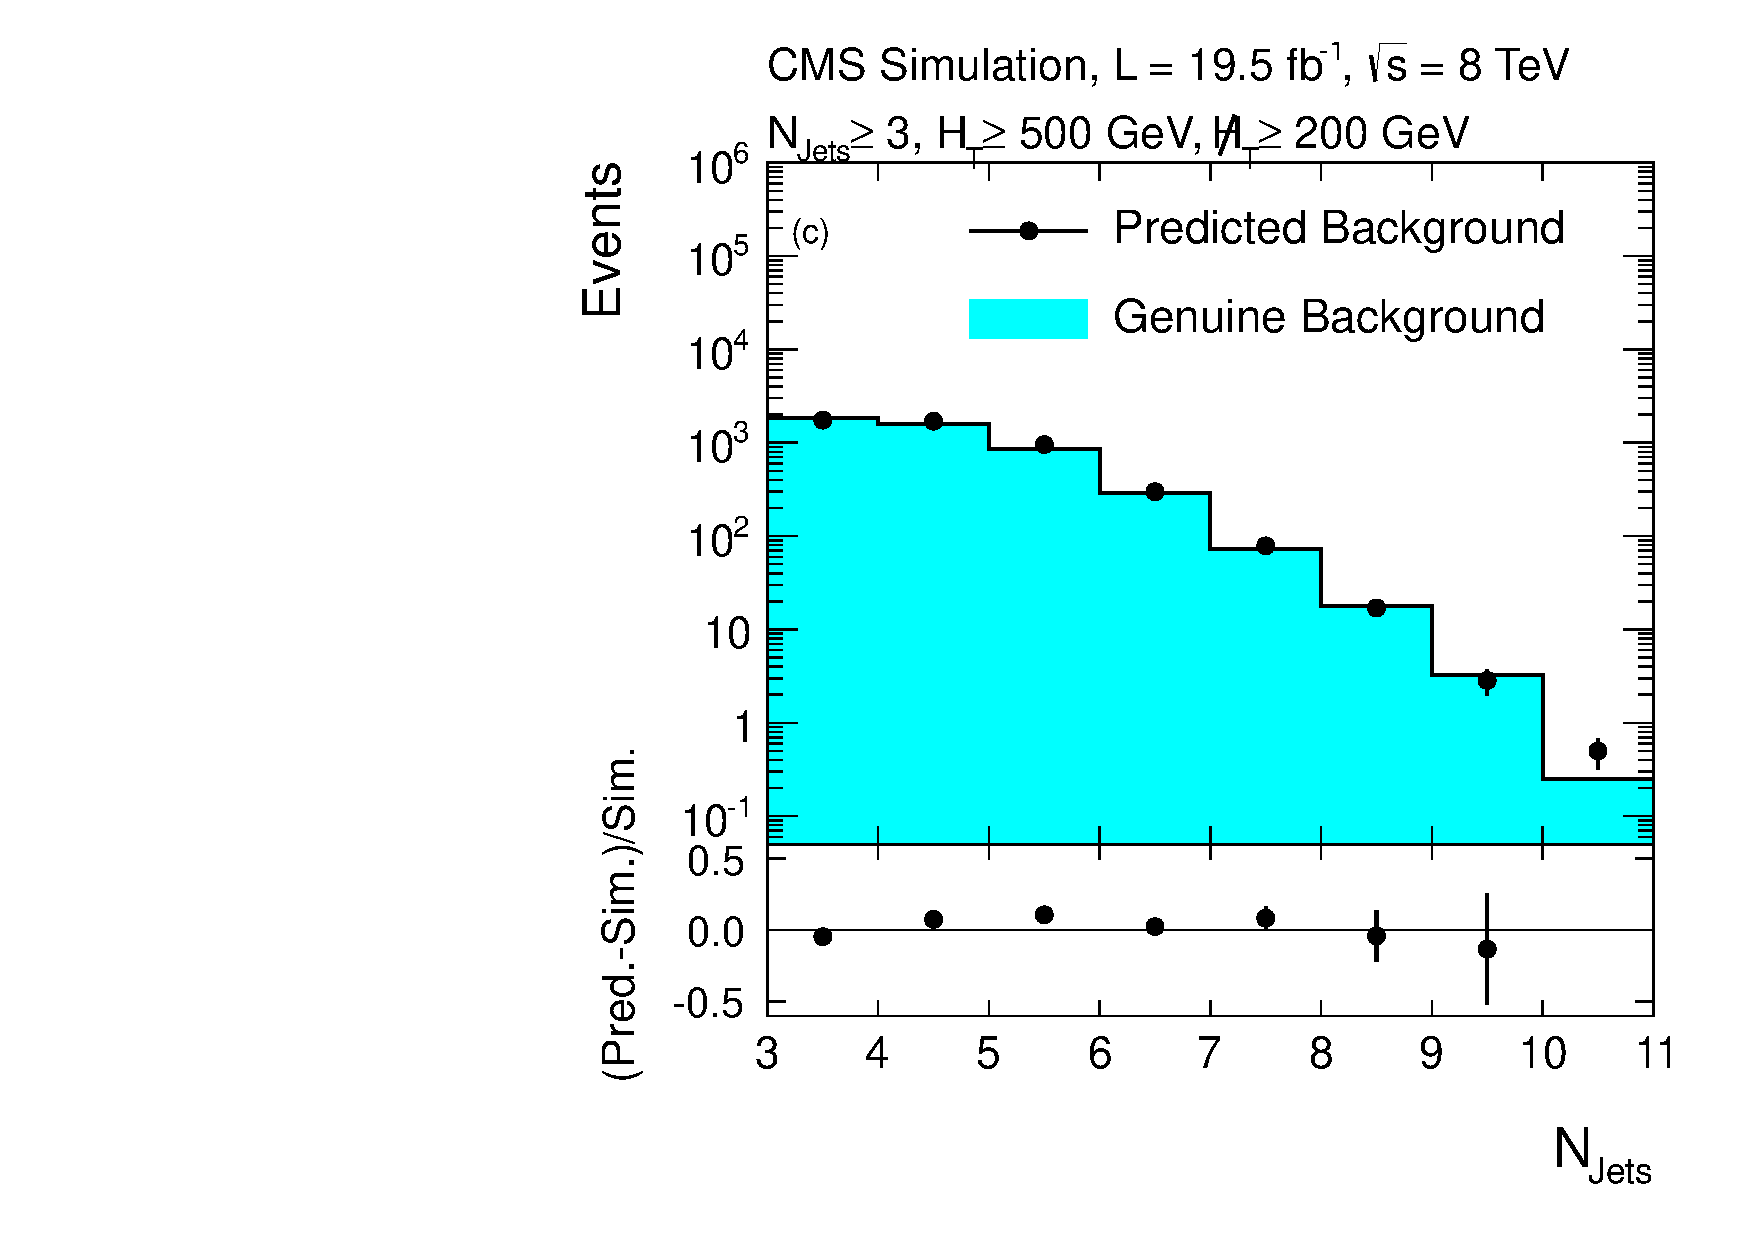
\includegraphics[width=0.49\textwidth]{figures/RA2_TauHad3.pdf}
    \end{center}
  \end{minipage}

  \caption{Predicted (a) \HT, (b) \MHT, and (c) \NJets distributions found from applying the hadronic-tau background evaluation method to simulated \ttbar and \WJets events (solid points) in comparison to the genuine \ttbar and \WJets background from simulation (shaded curve). Only statistical uncertainties are shown. Taken from~\cite{Chatrchyan:2014lfa}.}
  \label{fig:ra2_tauhad}
\end{figure}
Background contributions arising from \WJets and \ttbar events with a hadronically decaying $\tau$ lepton are estimated using a $\mu + \mathrm{jets}$ control sample. Since $\mu + \mathrm{jets}$ and $\tau_h + \mathrm{jets}$ events arise from the same physics process, they feature the same kinematics except for the different response of the detector to a $\mu$ and a $\tau_h$.  \\
The $\mu + \mathrm{jets}$ sample is selected by triggering on a single muon or a muon accompanied by at least two jets. Furthermore, instead of applying a lepton veto, exactly one $\mu$ with \pt$ > 20$\gev and $|\eta| < 2.1$ is required. In order to prevent the control sample from signal contamination a selection on the transverse mass $m_T = \sqrt{2\pt^{\mu}\met[1-\mathrm{cos(\Delta \phi)}]}$ of $m_T \le 100$\gev is imposed with the azimuthal angle $\Delta \phi$ between the direction of the muon four-momentum and the \met vector. \\
The difference between the $\mu$ and the $\tau_h$ is taken into account by replacing the muon by a simulated $\tau_h$ jet. This is done by randomly sampling the transverse momentum of the $\tau_h$ jet from the response $\pt^\mathrm{jet}/\pt^{\tau}$ obtained from simulation a reconstructed jet with $\pt^\mathrm{jet}$ to a generated hadronically decaying $\tau$ lepton with $\pt^{\tau}$ in the $(\eta, \phi)$-space. The generated $\tau$ lepton has to fulfill $\pt > 20$\gev and $|\eta| < 2.1$ and the distance for the matching is chosen to be $\Delta R < 0.2$ for tau-\pt$ < 50$\gev and $\Delta R < 0.1$ otherwise. The response is obtained from simulated \ttbar and \WJets events and subsequently mixed according to the cross sections of these processes in order to emulate what happens in data where both \ttbar and \WJets events occur. The random sampling of the response is repeated one hundred times for each event to sample the complete response function. If an event in the control sample is obtained from a prescaled trigger, the repetition of the sampling is increased according to the prescale factor. Technically, sampling means that the four-momentum of the muon is sclaed with the proper value from the $\tau_h$ response.  \\
In the following, \HT, \MHT and \NJets are recalculated for each event including the transverse momentum of the $\tau_h$ jet and all selection criteria as described in Sec.~\ref{subsec:RA2_baseline} are applied to the sample. The background contribution due to hadronic-$\tau$ events is obtained for all search regions by further correcting the event yields for the trigger efficiency, muon reconstruction and isolation efficiency, kinematic and detector acceptance as well as the ratio of branching fractions of $W \rightarrow \tau_h \nu$ to $W \rightarrow \mu \nu$ events. The statistical uncertainty of the background prediction is estimated with pseudo-experiments using a bootstrap method~\cite{GVK017474957}. \\
The validity of this background estimation procedure is tested by comparing the event yields obtained from applying the prediction method to simulated events from \ttbar and \WJets events to the respective genuine background. This comparison is shown as function of \HT, \MHT and \NJets in Fig.~\ref{fig:ra2_tauhad} after the baseline selection. Although the agreement is quite reasonable and hence the method is supposed to work reliable, uncertainties of 10\% are considered for $\NJets = 3 - 5$ and 20\% for jet multiplicities $\NJets = 6 - 7$ and $\NJets \ge 8$. These uncertainties mainly reflect the statistical precision of the validation test. \\
Further systematic uncertainties taken into account for the hadronic $\tau$ background prediction are covering differences in data and MC for the muon isolation and reconstruction efficiencies as well as uncertainties on the kinematic and geometric acceptance, the $\tau_h$ jet response and the acceptance of the transverse mass cut. 

%\begin{figure}[!t]
%  \centering
%\makebox[\linewidth]{
%  \begin{tabular}{ccc}
%                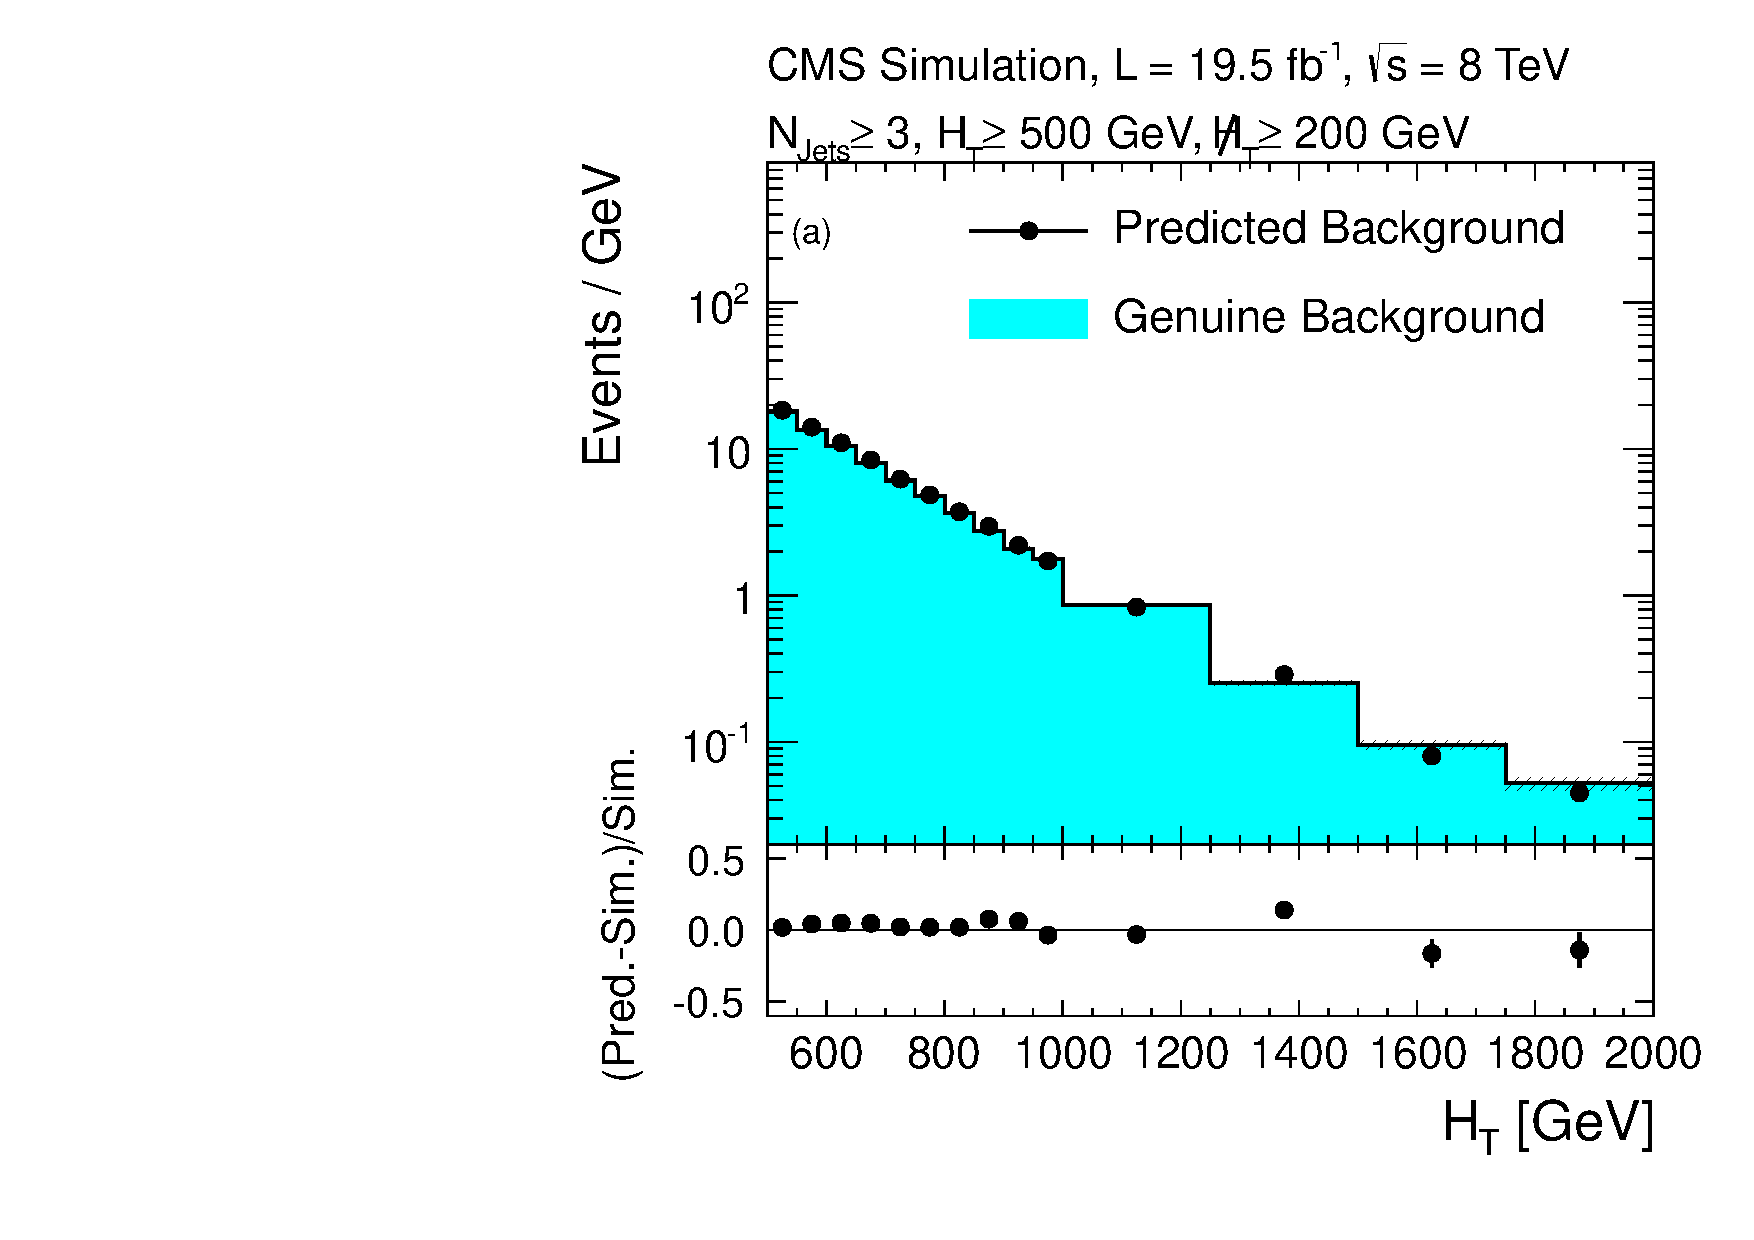
\includegraphics[width=0.4\textwidth]{figures/RA2_TauHad1.pdf} & 
%                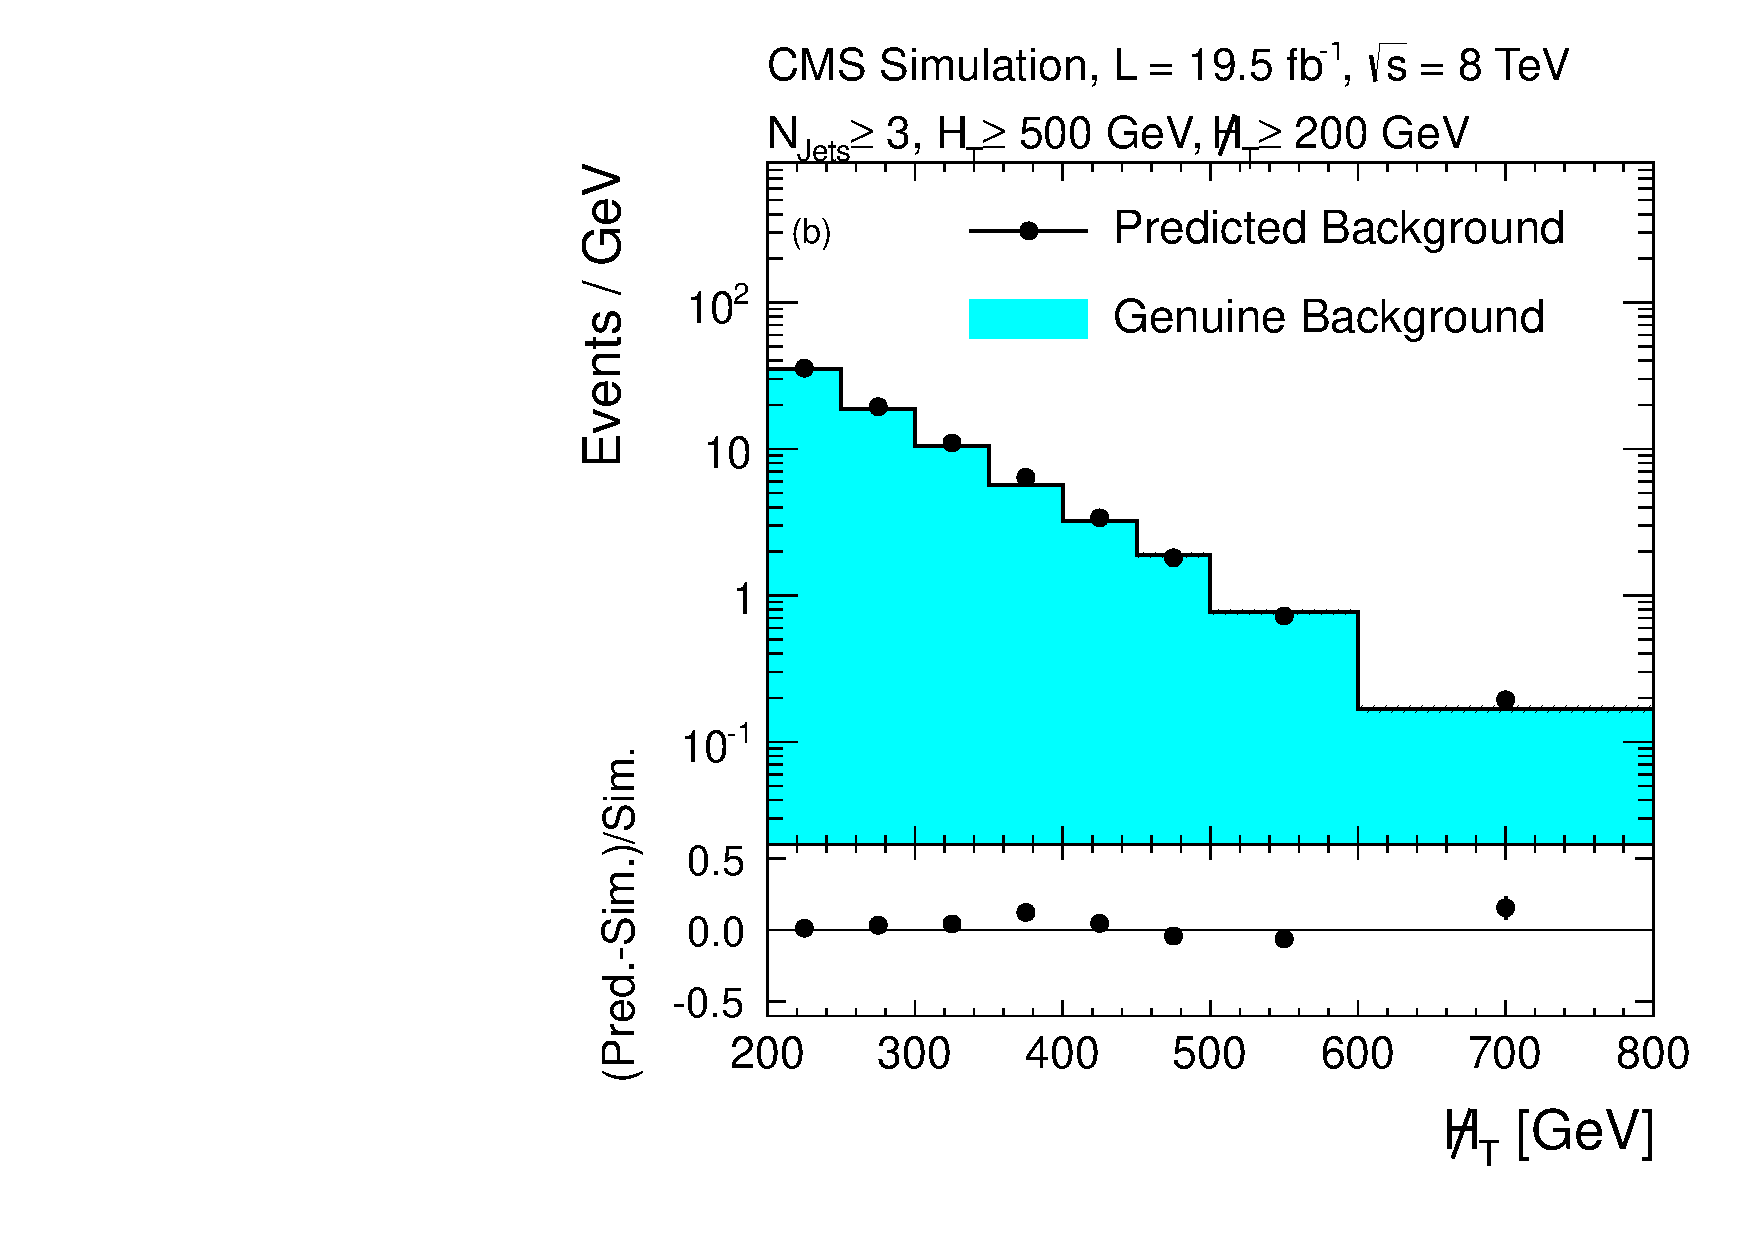
\includegraphics[width=0.4\textwidth]{figures/RA2_TauHad2.pdf} &
%                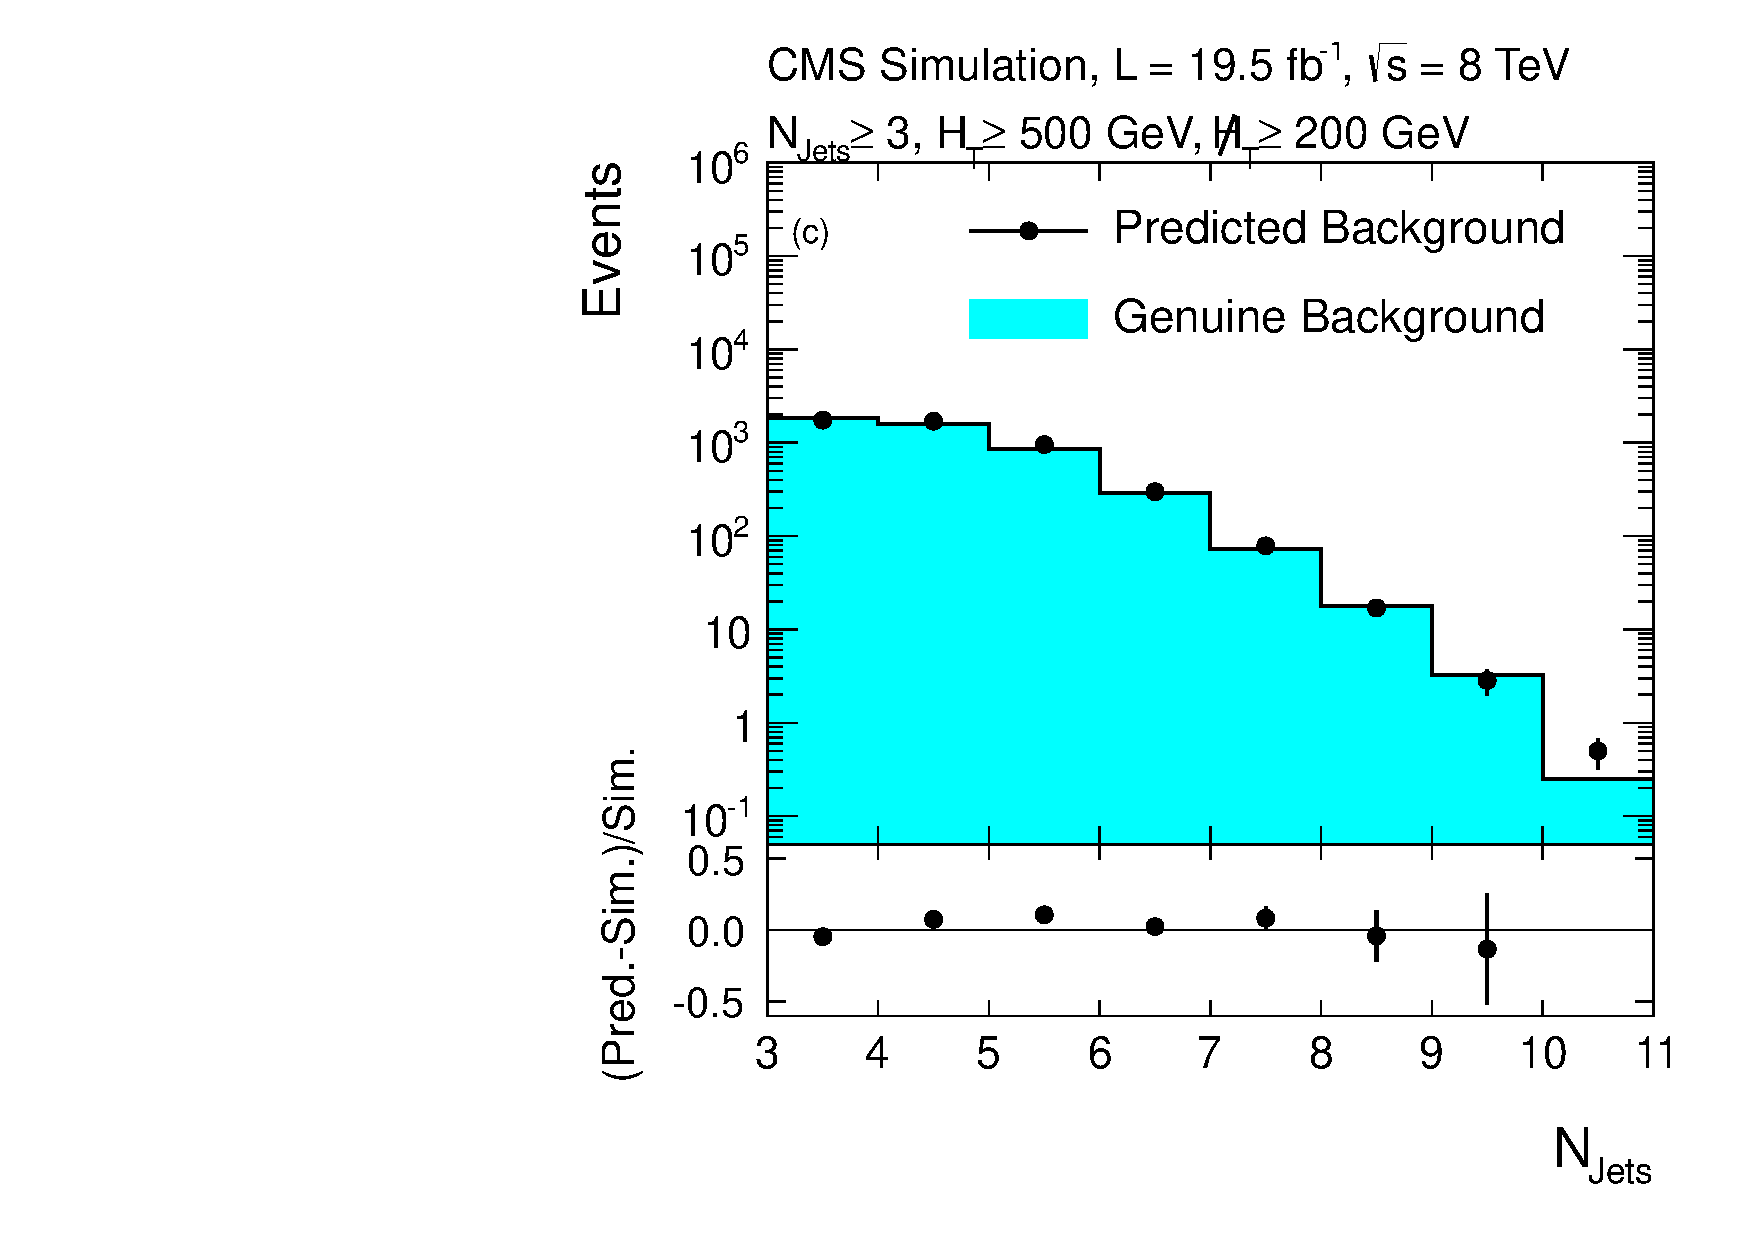
\includegraphics[width=0.4\textwidth]{figures/RA2_TauHad3.pdf}
%  \end{tabular}}
%  \caption{Predicted (a) \HT, (b) \MHT, and (c) \NJets distributions found from applying the hadronic-tau background evaluation method to simulated \ttbar and \WJets events (solid points) in comparison to the genuine \ttbar and \WJets background from simulation (shaded curve). Only statistical uncertainties are shown. Taken from~\cite{Chatrchyan:2014lfa}.}
%  \label{fig:ra2_tauhad}
%\end{figure}

\subsection{Lost-Lepton Background}
\label{subsec:RA2_lostlepton}
\begin{figure}[!t]
  \centering

  \begin{minipage}[c]{1.\textwidth}
    \begin{center}
      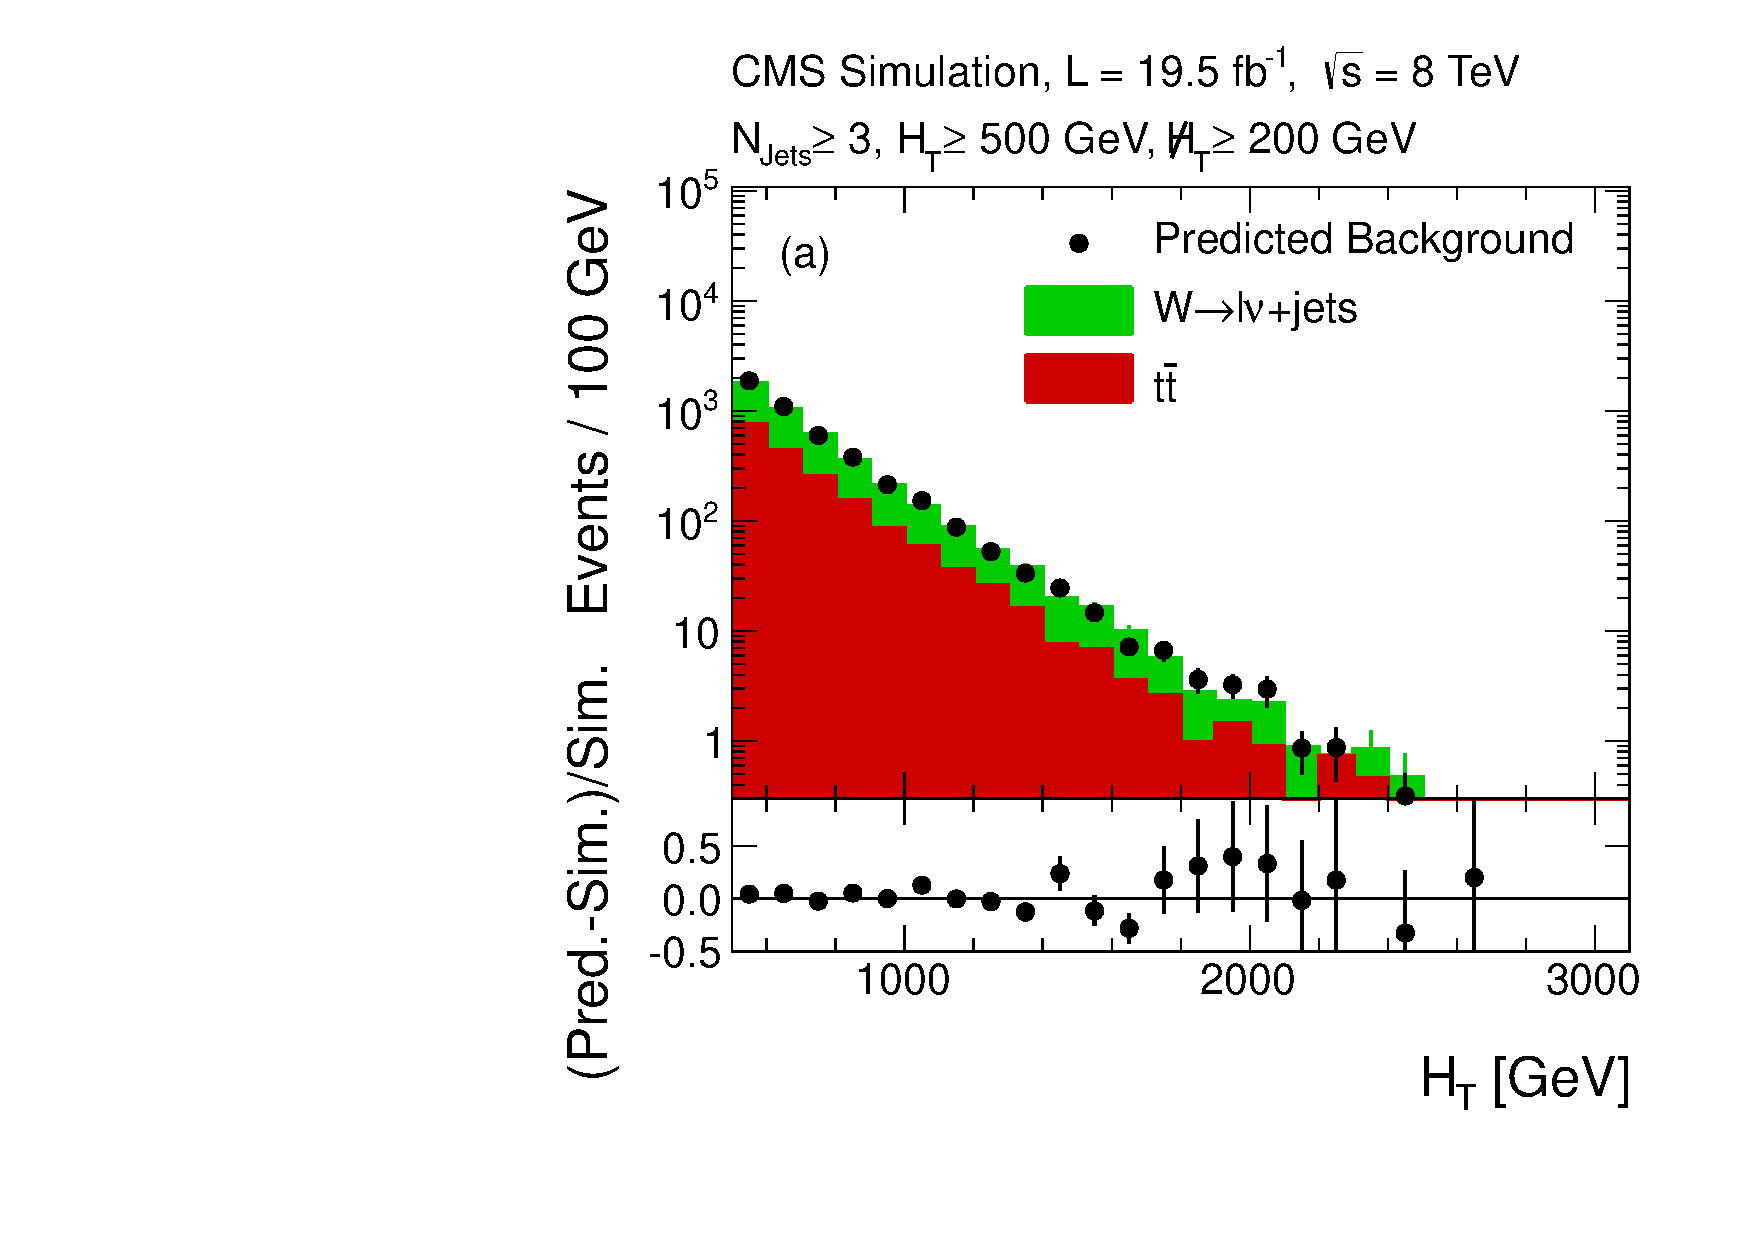
\includegraphics[width=0.49\textwidth]{figures/RA2_LL1.pdf}% \hspace {1.5 pt} 
      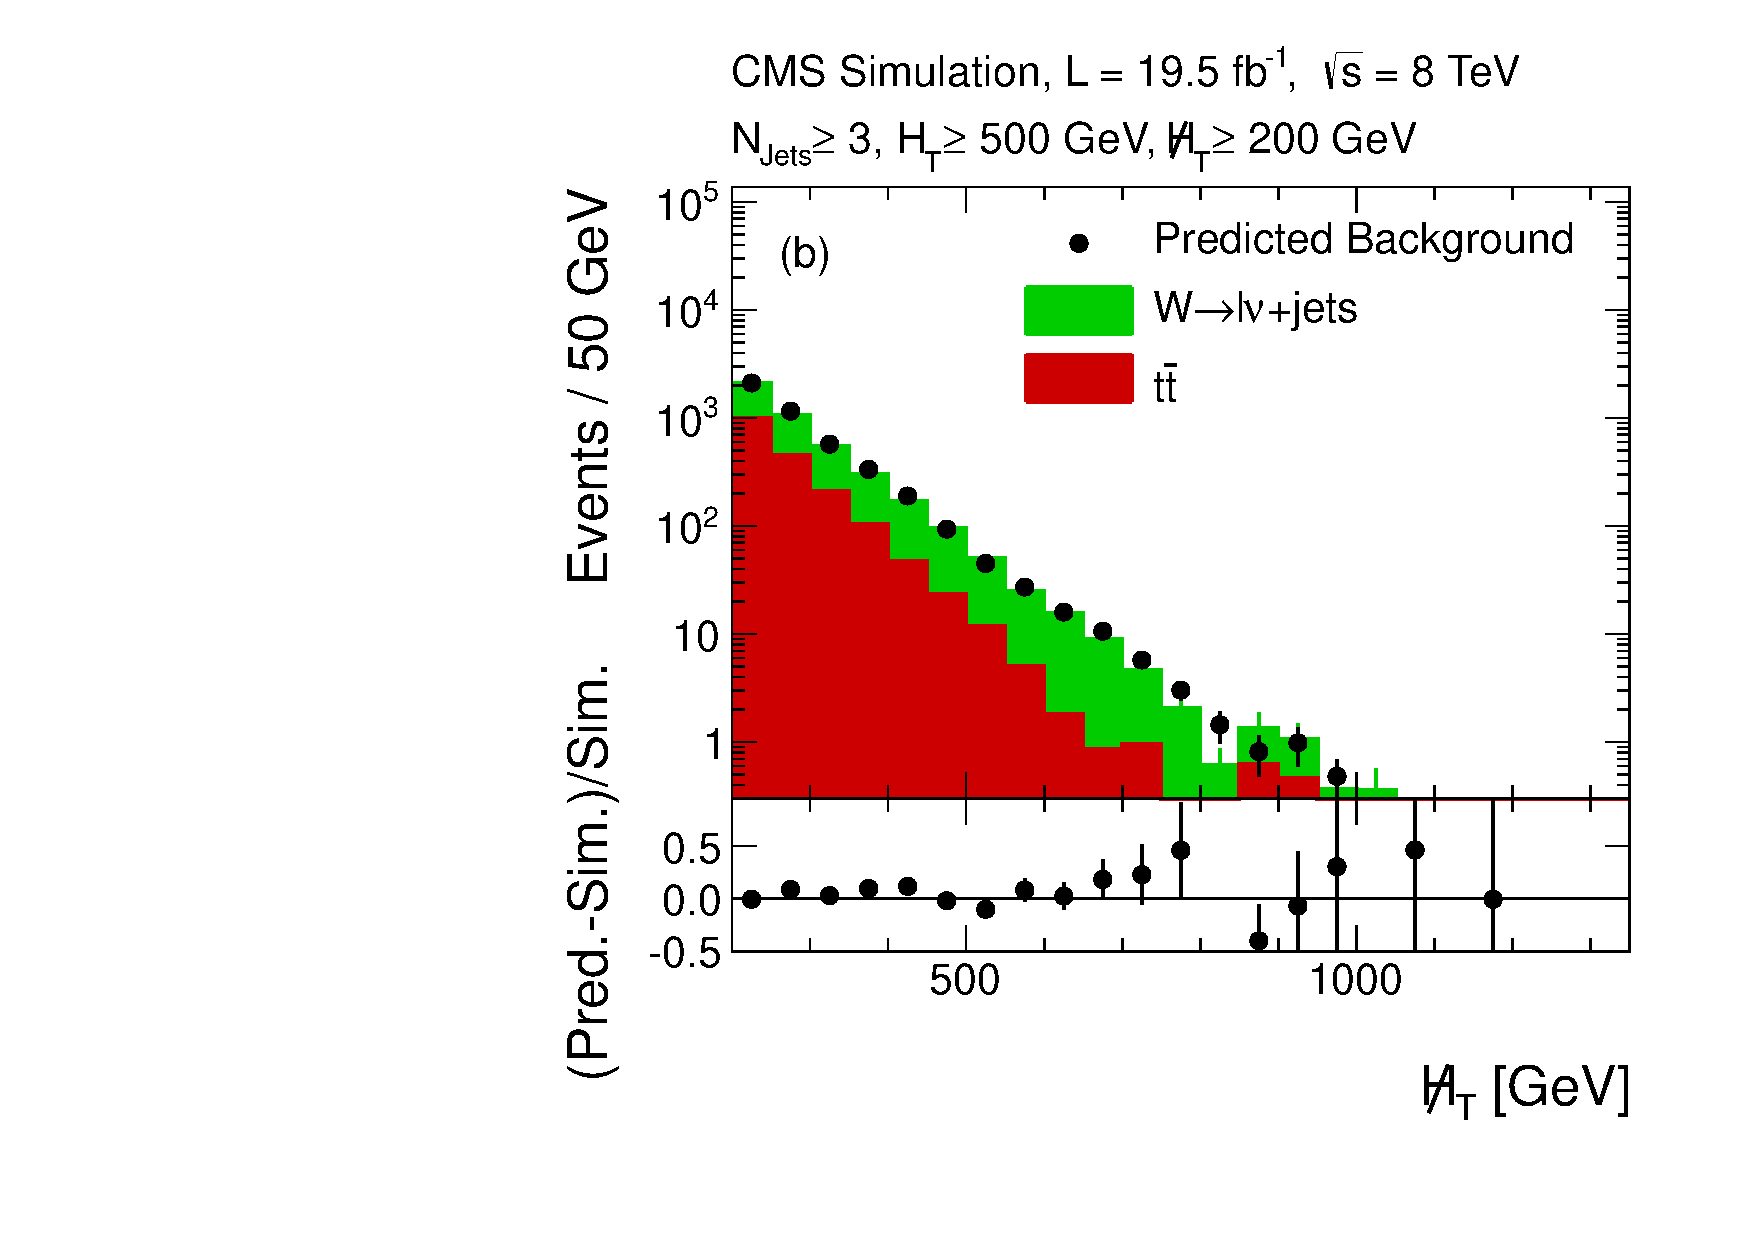
\includegraphics[width=0.49\textwidth]{figures/RA2_LL2.pdf}\\ 
      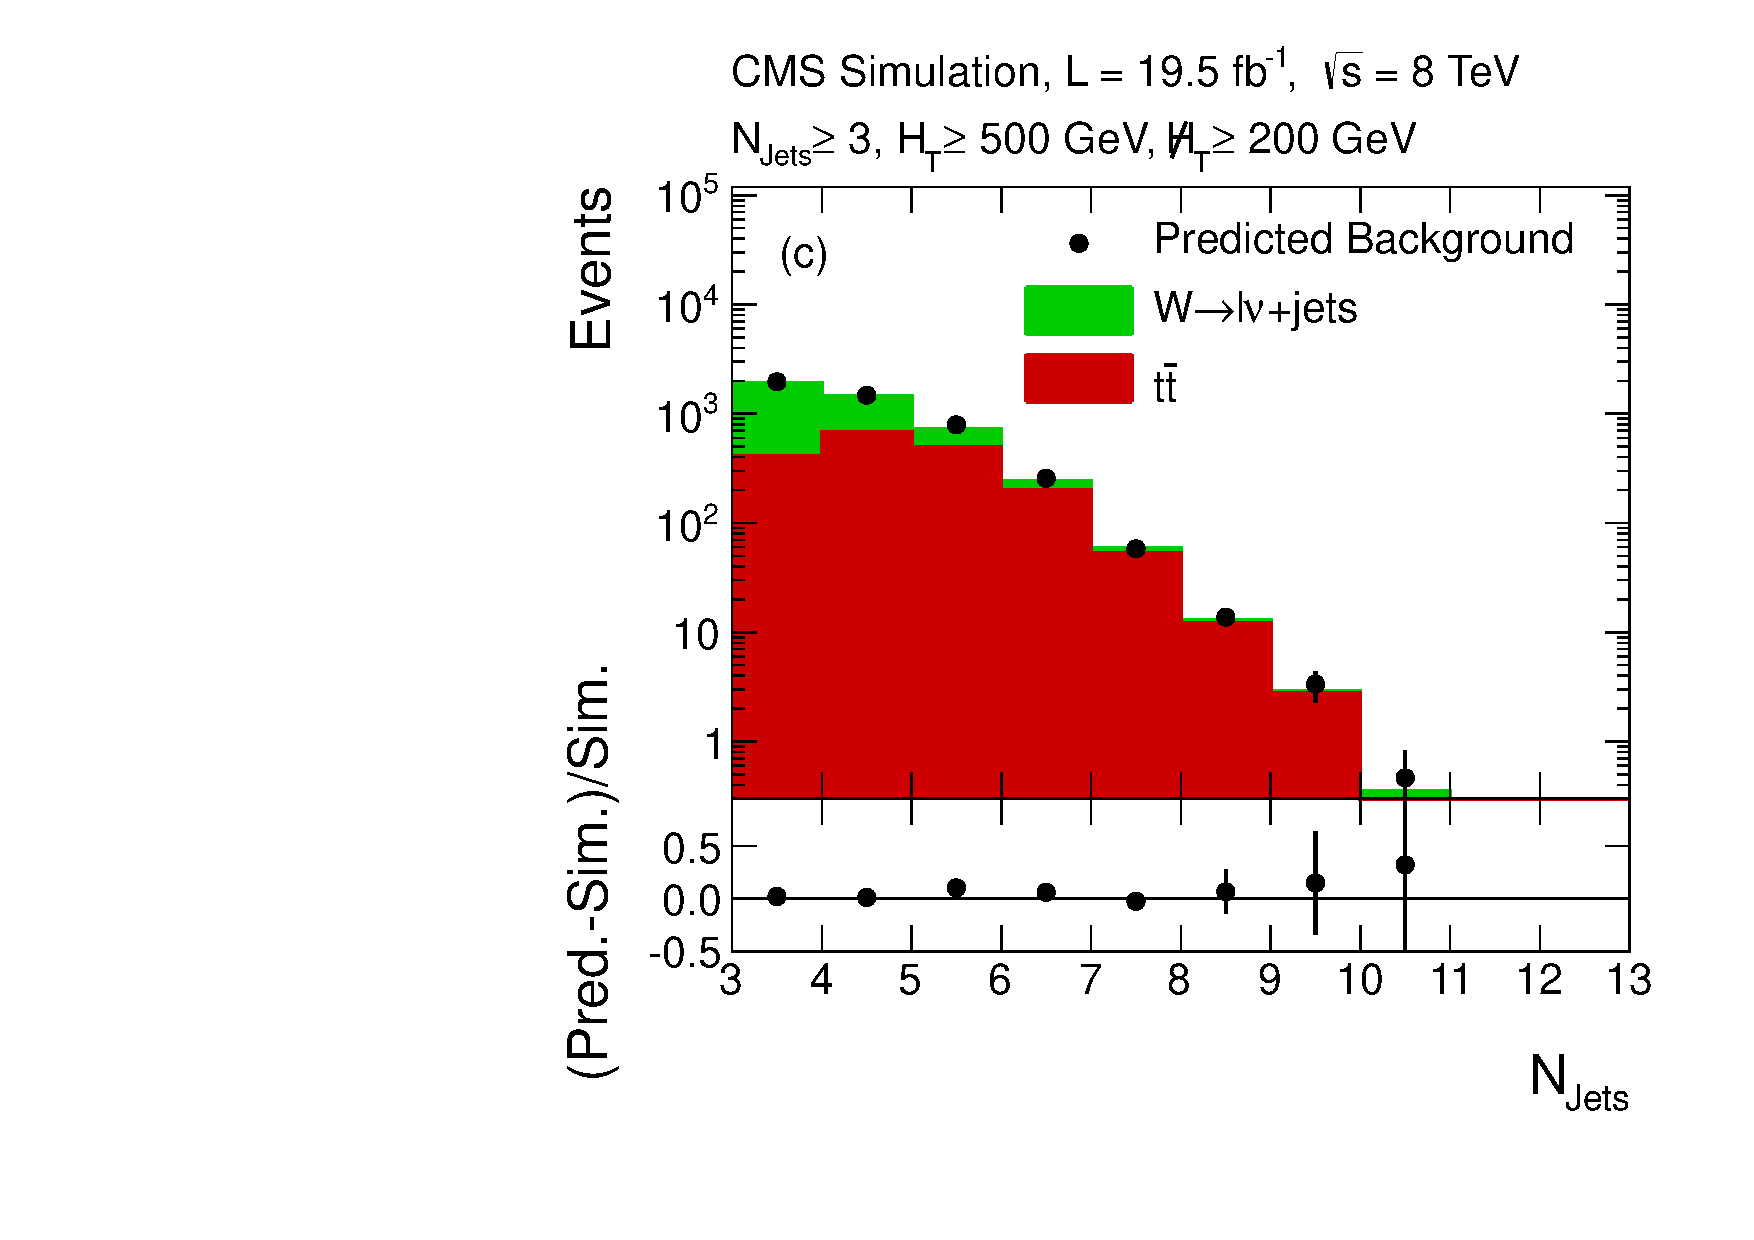
\includegraphics[width=0.49\textwidth]{figures/RA2_LL3.pdf}
    \end{center}
  \end{minipage}

  \caption{Predicted (a) \HT, (b) \MHT, and (c) \NJets distributions found from applying the lost lepton background evaluation method to simulated \ttbar and \WJets events (solid points) in comparison to the genuine \ttbar and \WJets background from simulation (shaded curves). Only statistical uncertainties are shown. Taken from~\cite{Chatrchyan:2014lfa}.}
  \label{fig:ra2_ll}
\end{figure}
Similar to background events from hadronic tau decays, the background contribution due to a failed veto of a light lepton is estimated from a $\mu + \mathrm{jets}$ control sample. This is selected with the same trigger as used for the search. The sample is selected by requiring exactly one well-reconstructed and isolated muon with $\pt > 10$\gev. Furthermore, the same transverse mass requirement of $m_T < 100$\gev as for the hadronic tau background is applied. \\ 
The number of events in the zero-lepton search regions can be estimated from the single-muon sample by weighting the events according to the lepton reconstruction and isolation efficiencies as well as the detector and kinematic acceptance of the muons. The respective efficiencies and acceptances are obtained from simulated \ttbar and \WJets events and determined in intervals of \HT, \MHT and \NJets. \\
In order to determine the number of events due to unidentified leptons the events in the control sample are weighted according to
\begin{equation*}
\frac{1}{\epsilon_\mathrm{iso}^\mathrm{\mu}} \times \frac{1-\epsilon_\mathrm{reco}^{e, \mu}}{\epsilon_\mathrm{reco}^{\mu}}
\end{equation*}
and with
\begin{equation*}
\frac{\epsilon_\mathrm{reco}^{e, \mu}}{\epsilon_\mathrm{reco}^{\mu}} \times \frac{1-\epsilon_\mathrm{iso}^{e, \mu}}{\epsilon_\mathrm{iso}^{\mu}}
\end{equation*}
to account for non-isolated leptons. Both equations are based on the reconstruction $\epsilon_\mathrm{reco}^{e, \mu}$ and isolation $\epsilon_\mathrm{iso}^{e, \mu}$ efficiencies of the electron and muon, respectively. 
The method is validated in simulation by comparing the predicted event yields for lost-lepton events in \ttbar and \WJets from a signle-muon control sample after the baseline selection to the genuine background. This comparison is illustrated in Fig.~\ref{fig:ra2_ll} as function of \HT, \MHT and \NJets and shows a good overall agreement. An uncertainty of 15\% is assigned to jet multiplicities 3--5 and 40\% to the others in order to account for the statistical precision of this validation test.\\
Main other uncertainties of the lost-lepton background prediction arise from the lack of sufficient events in the control sample in each defined search region, differences in lepton reconstruction and isolation efficiency between data and simulation, impact on the acceptance when varying the used PDFs and the acceptance of the transverse mass cut.

%\begin{figure}[!t]
%  \centering
%\makebox[\linewidth]{
%  \begin{tabular}{ccc}
%                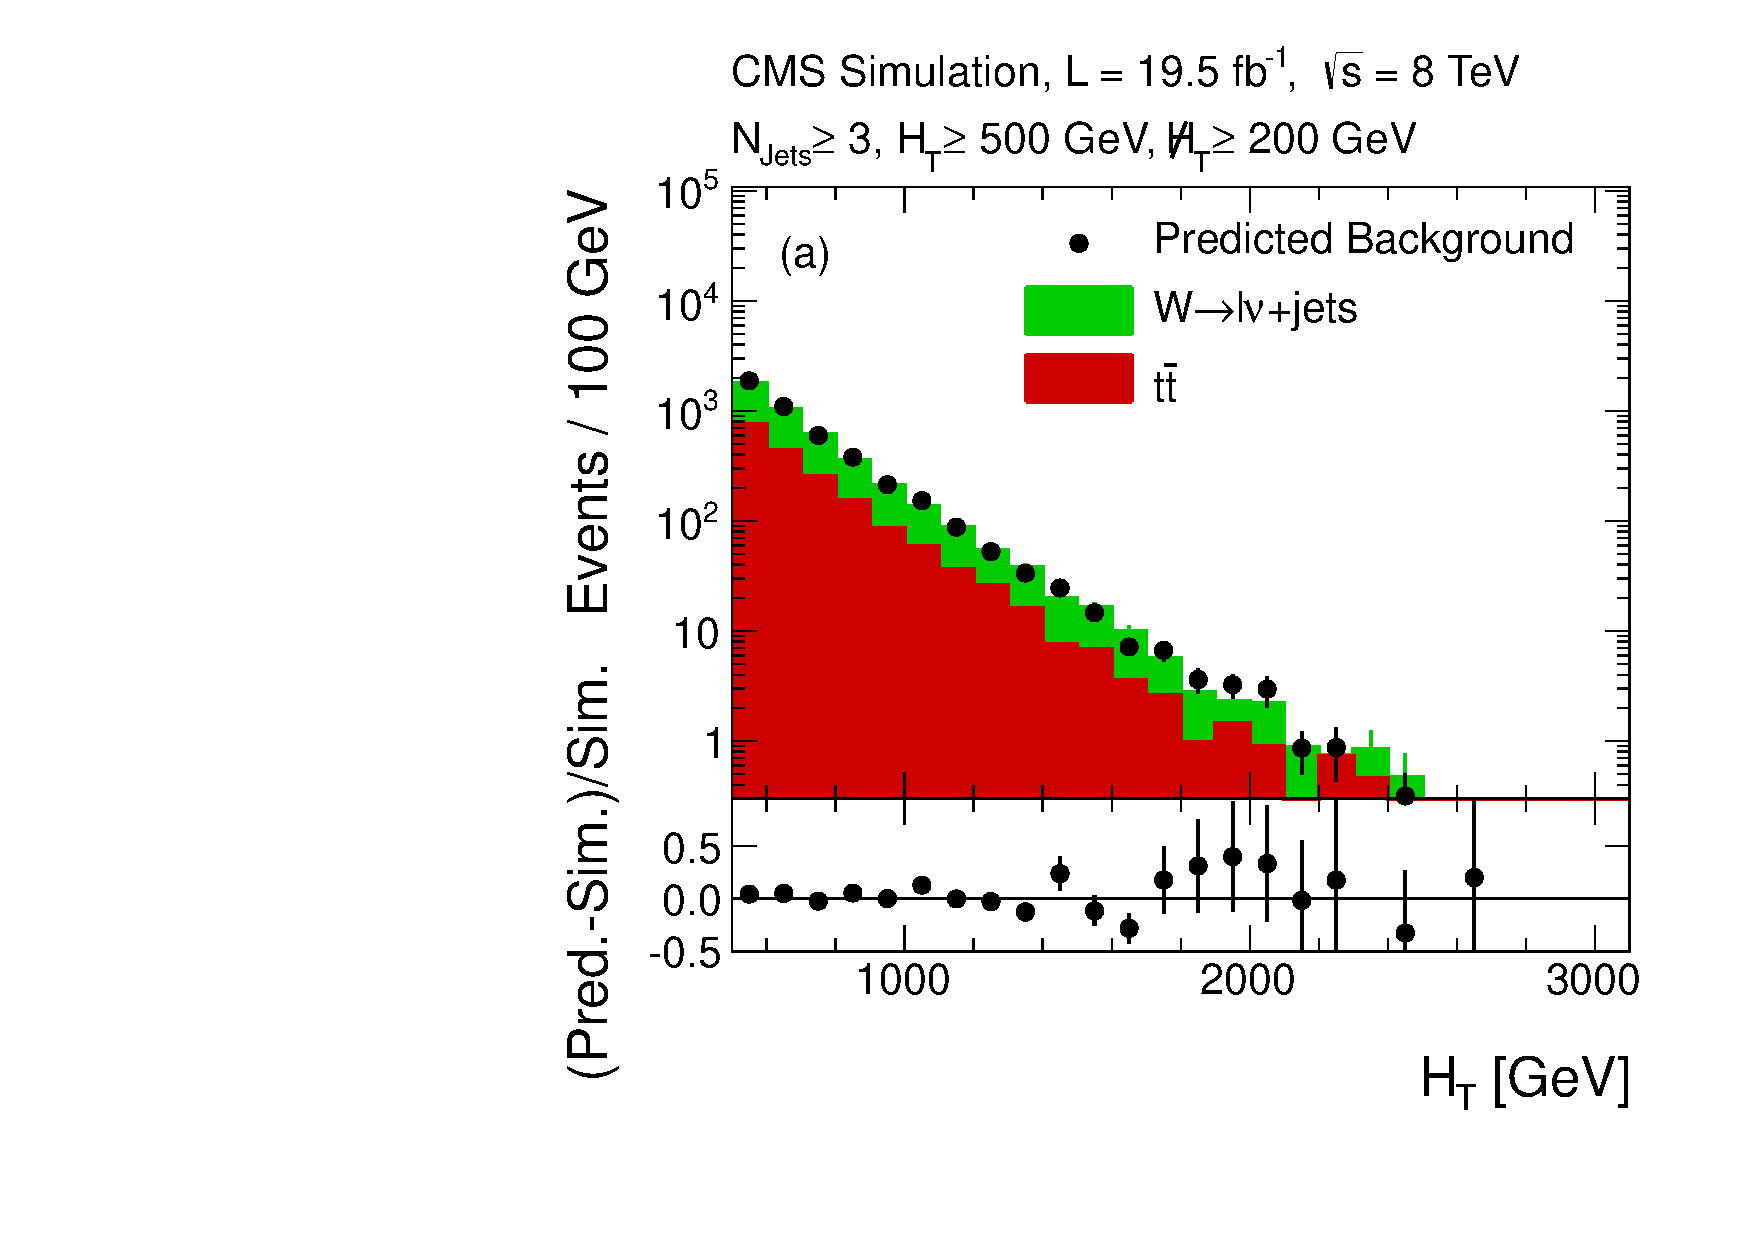
\includegraphics[width=0.4\textwidth]{figures/RA2_LL1.pdf} & 
%                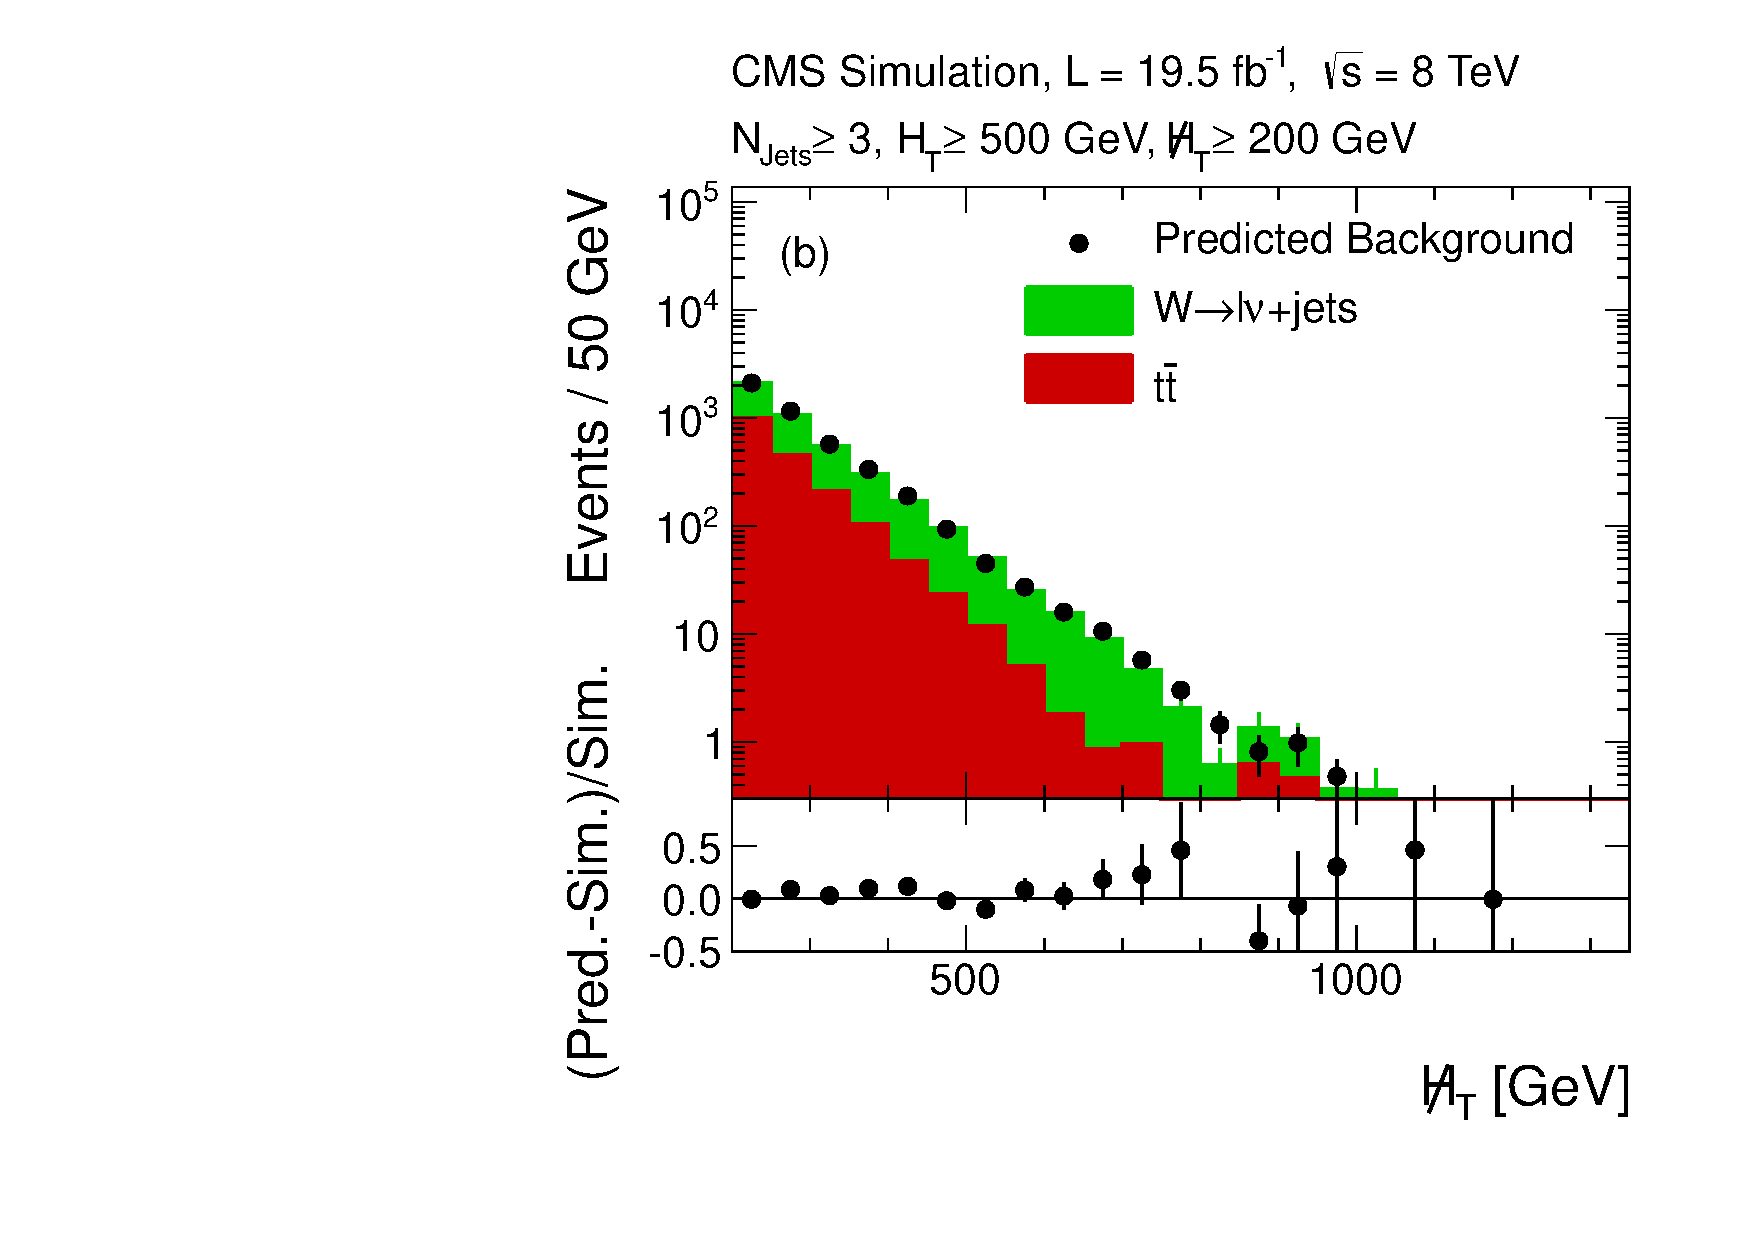
\includegraphics[width=0.4\textwidth]{figures/RA2_LL2.pdf} &
%                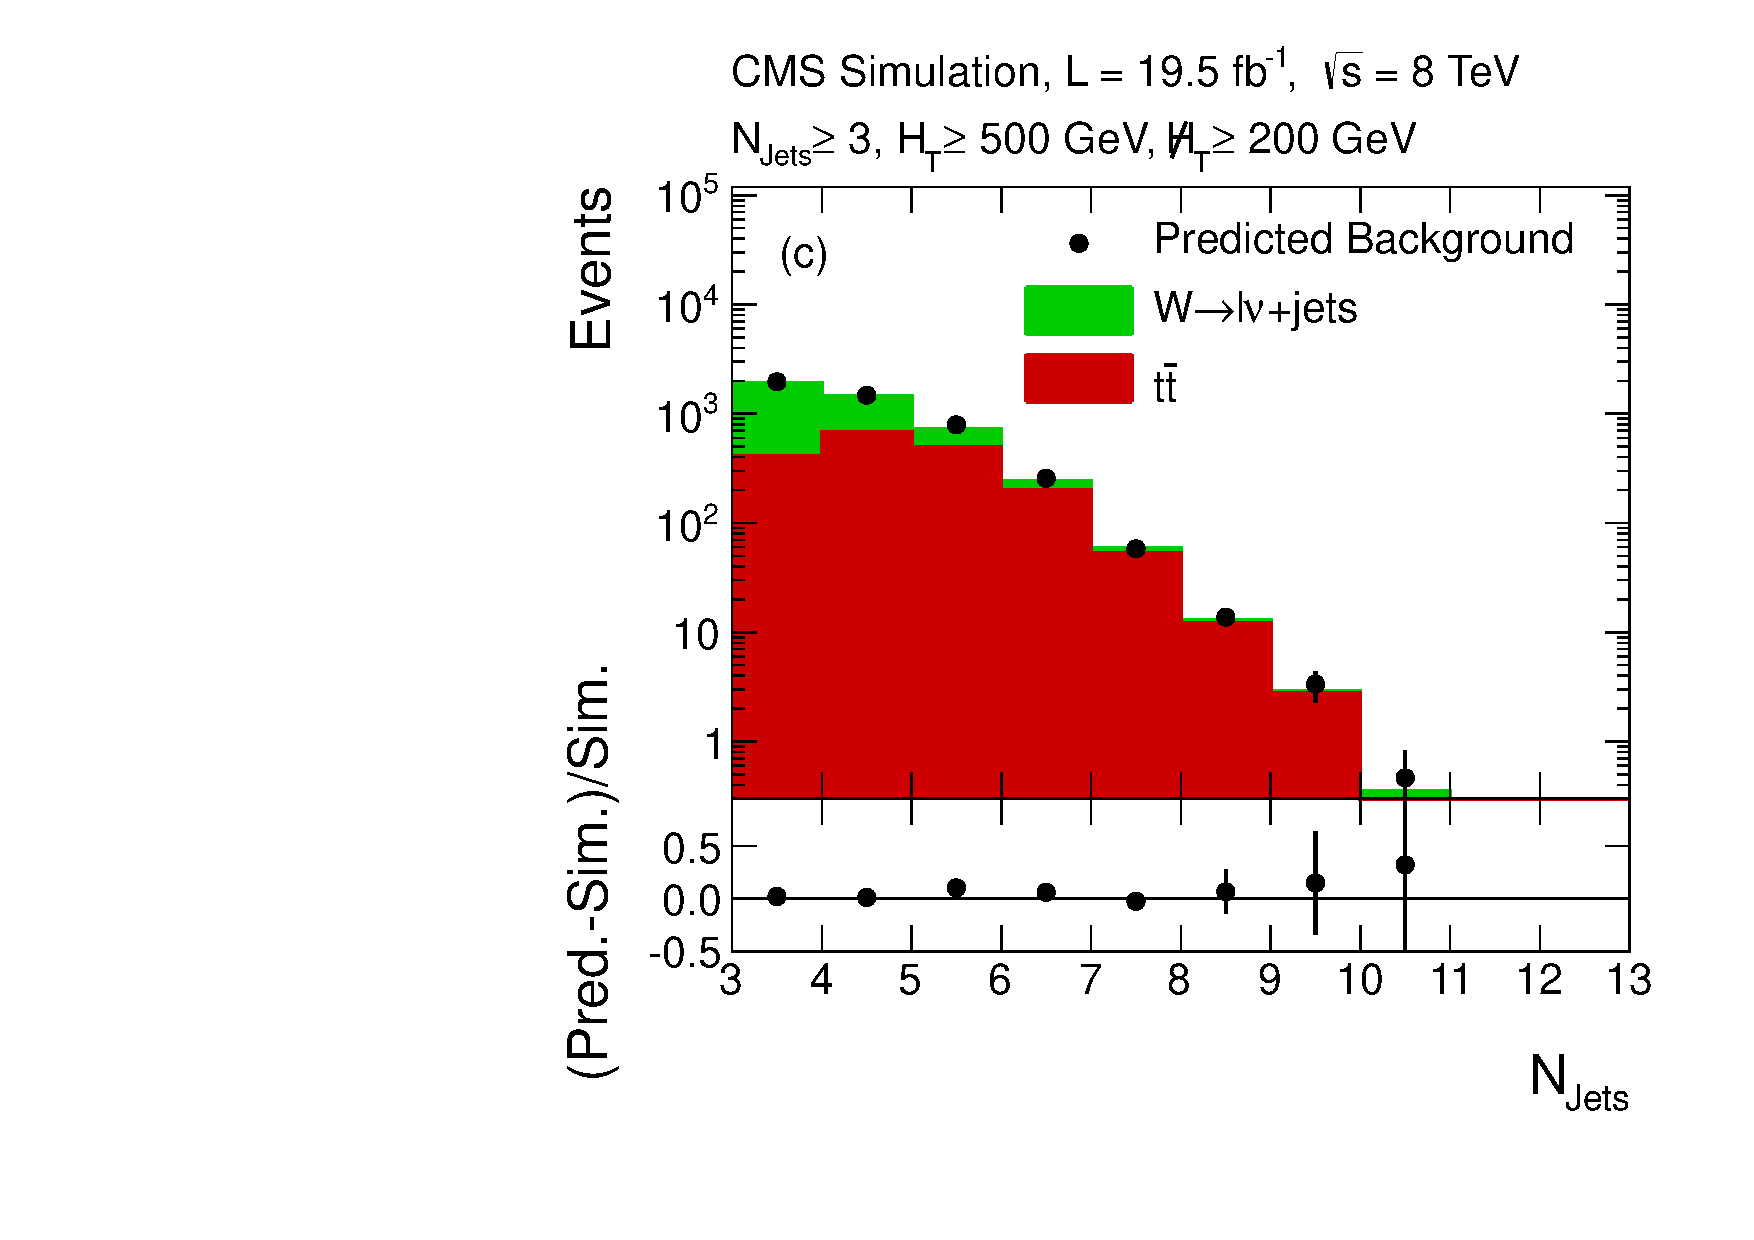
\includegraphics[width=0.4\textwidth]{figures/RA2_LL3.pdf}
%  \end{tabular}}
%  \caption{Predicted (a) \HT, (b) \MHT, and (c) \NJets distributions found from applying the lost lepton background evaluation method to simulated \ttbar and \WJets events (solid points) in comparison to the genuine \ttbar and \WJets background from simulation (shaded curves). Only statistical uncertainties are shown. Taken from~\cite{Chatrchyan:2014lfa}.}
%  \label{fig:ra2_ll}
%\end{figure}

\section{QCD Background Estimation with the Rebalance-And-Smear Method}
\label{subsec:RA2_QCD}
Background contributions arising from events with no intrinsic missing energy, except for neutrinos in jets arising for instance from electroweak decays of heavy-flavour quarks, are estimated with the \textit{Rebalance-and-Smear} (R+S) method. The main contribution is caused by QCD multijet events which also caused the naming 'QCD background'. However, minor contributions originate also from fully-hadronic decaying \ttbar, \WJets and \ZJets events. The high values of missing transverse energy which cause these events to contribute to the analysed signal regions is consequently arising from severe jet mismeasurements. \\
Typically, QCD background is the most difficult background to model for all-hadronic SUSY searches, as a precise description of the underlying particle-level jet spectrum is needed and how this manifests in the detector. Especially the former suffers from large theoretical uncertainties in particular in the extreme kinematic phase space the analysis is performed in. To overcome this, the data-based R+S-method was developed and already successfully used in previous analyses~\cite{springerlink:10.1007/JHEP08(2011)155, Chatrchyan:2012lia}. In this thesis, particularly improvements of the R+S method are discussed that became inevitable to handle the main changes of this analysis at $\sqrt{s} = 8$\tev manifesting in the extension of the search regions in several jet mulitplicities and the increased amount of pileup compared to the 7\tev analyses. Consequently, the R+S method is adjusted such that it leads to precise results regarding also this new conditions. In general, the method is based on the assumption that if the momenta of particle-level jets in an event are known, the reconstructed jet momenta can be modelled by a per-jet resolution function.  \\
After the discussion of the general concept of the R+S method in Sec.~\ref{subsec:RPlusS_concept}, the adjustment of the procedure to the actual conditions for 8\tev data are introduced in Sec.~\ref{subsec:RPlusS_app}. Furthermore, systematic uncertainties are discussed in Sec.~\ref{subsec:RA2_syst_unc} and the results of the actual QCD background prediction are presented in Sec.~\ref{subsec:RA2_qcd_pred}. 

\subsection{General concept of the Rebalance-and-Smear method}
\label{subsec:RPlusS_concept} 
As stated above, QCD background contributions arise from jet mismeasurements in the detector. Thus, this background contribution can be estimated by retracing the measurement of multijet events. In order to do this, the prediction of the QCD background is performed in two subsequent steps. First, the events are \textit{rebalanced}, as described below, such that the missing energy in the event is removed and almost ideal multijet events denoted \textit{seed events} are obtained. The resulting seed events reflect the event kinematics before the actual detector measurement is performed and are thus estimators of the true particle-level jet momenta. In a second step, all jets in the event are \textit{smeared} with the full jet response function, \ie jet momenta are scaled with a factor randomly drawn according to the jet response distribution, to model the interaction of the multijet state with the detector. Smeared events contain the whole event kinematics of the studied background contribution, such that these can be used to derive contributions to various kinematic distributions, like \HT or \MHT, so that the R+S method can be used to really predict event kinematics rather than only event counts for the selected search regions. The general outline of the R+S method is illustrated in Fig.~\ref{fig:RPlusS_concept}.
\begin{figure}[!t]
  \centering
  \makebox[\linewidth]{
  \begin{tabular}{c}
                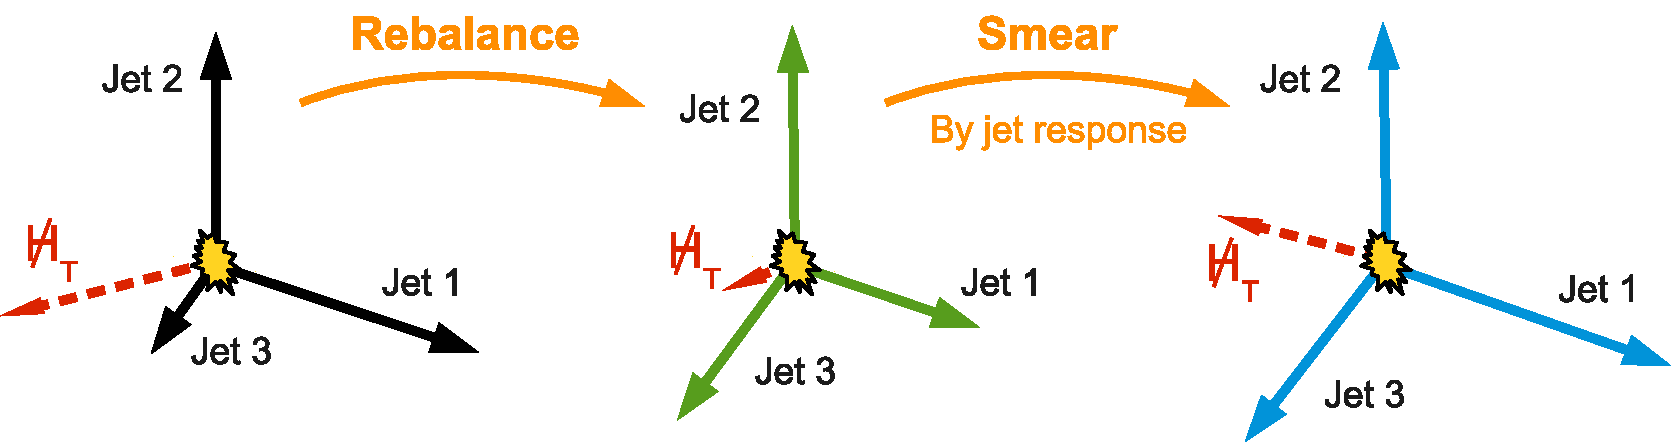
\includegraphics[width=0.99\textwidth]{figures/SketchJetSmearingMethod_LabelMHT.pdf}  
  \end{tabular}}
  \caption{Outline of the two steps performed in the R+S method for estimation of QCD background events. Sketch provided by~\cite{MSchrode}.}
  \label{fig:RPlusS_concept}
\end{figure}
\begin{description}
 \item \textbf{Reponse Templates:}
As indicated above, the R+S method crucially relies on a precise parametrization of the jet response to both perform the rebalancing and the jet smearing. The MC-truth response is derived for simulated QCD multijet events with the full detector simulation for $\pt^\mathrm{gen}$ and $|\eta^\mathrm{gen}|$ intervals summarized in Tab.~\ref{tab:RPlusS_binning}. Although a very fine binning is chosen, the response in each interval is averaged over a certain part of the $\pt^\mathrm{ave}$ spectrum. Thus, the response distribution tends to overestimate the width of the resolution for high-\pt jets while it behaves the other way round for low-\pt jets. Reconstructed jets at detector-level are AK5 jets with charged-hadron subtraction applied and calibrated according to the description in Sec.~\ref{subsec:jets_calib}. Furthermore, the pileup scenario of the simulated sample is reweighted to match the one observed in data, as explained in Sec.~\ref{subsec:jer_sel_cuts}. \\
As explained in Sec.~\ref{sec:jer_response}, the truth jet response is derived by performing an unambigous matching of reconstructed jet $i$ to generated jet $i$ using here $\Delta R < 0.1$. In order to avoid tails from splitiing and merging effects of the jet reconstruction, any further reconstructed or generated jet $j \ne i$ around a matched pair is vetoed in a cone of size $R < 0.7$ by requiring
\begin{equation}
 \pt^{\rm{GenJet}_j} / \pt^{\rm{GenJet}_i} < 0.05
\end{equation} 
and
\begin{equation}
 \pt^{\rm{Jet}_j} < 30\,\mathrm{GeV} \;\; \mathrm{and} \;\; \pt^{\rm{Jet}_j} / \pt^{\rm{Jet}_i} < 0.05 \; .
\end{equation} 
The obtained jet response distributions are averaged over all jets in an event not separating them according to their rank, \ie their position in a descending \pt order, or according to the jet flavour. Thus, the flavour composition reflects that of an average QCD multijet sample. 
\begin{table}[!t]
\centering
\caption{Overview of the $|\eta^\mathrm{gen}|$ and $\pt^\mathrm{gen}$ interval boundaries used for the MC-truth response determination used as input for the R+S method.}
\label{tab:RPlusS_binning}
\makebox[\linewidth]{
\begin{tabular}{c}
\multicolumn{1}{c}{} \\
\toprule
 $|\eta^\mathrm{gen}|$ \\
 0, 0.3, 0.5, 0.8, 1.1, 1.4, 1.7, 2.0, 2.3, 2.8, 3.2, 4.1, 5.0 \\
\midrule
$\pt^\mathrm{gen} \; [\mathrm{GeV}]$ \\
0, 20, 30, 50, 80, 120, 170, 230, 300, 380, \\
470, 570, 680, 800, 1000, 1300, 1700, 2200, 2800, 3500 \\
\bottomrule
\end{tabular}}
\end{table} 
\\
The truth response templates to be used for applying the R+S method in simulated events, \eg for validation tests, are determined as described above. However, when using the truth response templates for the actual QCD background predictions in data, they have to be corrected for potential data to simulation jet resolution differences. As seen in Chap.~\ref{chap:Resolution}, the resolution in data is typically worse than in simulation. Thus, the determined truth response templates are adjusted accordingly. This correction is done for the Gaussian core and the non-Gaussian tails separately. First, the response function is splitted into the respective core and tail parts. This is done by fitting the response distribution with a Gaussian in the range of $\pm$ 1\,RMS around the mean which is then subtracted from the total response distribution in order to obtain the tail parts and vice versa. The correction factors for the core resolution are applied by convoluting the MC-truth response with a Gaussian of width $\sigma_{c}$ according to Eq.~\ref{eq:res_adjust}. The considered correction factors are listed in Tab.~\ref{tab:jer_RPlusS_core} in the appendix and correspond to the data-to-simulation ratios obtained from dijet data at $\sqrt{s} = 7$\tev, as illustrated in Fig.~\ref{fig:result_comparison} (right).\footnote{Although the correction factors for the data-to-simulation ratio derived in the context of this thesis are more precise, these have not been available at that time when the analysis presented in this chapter has been performed.} The residual tail contributions are scaled according to the correction factors $\rho_\mathrm{tail}$ listed in Tab.~\ref{tab:jer_RPlusS_tails} in the appendix derived from dijet asymmetry parts fulfilling $(\mathcal{A} > 2 \sigma_c)$~\cite{thesis:Schroeder}.   

 \item \textbf{Rebalance Procedure:}
As stated above, the first step in the R+S method is to create a sample of seed events that serve as estimator of the true particle-level jets by performing a rebalancing of the multijet events. This rebalancing is done based on a \textit{kinematic fit}~\cite{D'Hondt:926540}. \\
This is based on the hypothesis that for a given event all measured and unmeasured quantities fulfill certain kinematic constraints, like energy and momentum conservation. However, due to the uncertainties of these quantities the constraints are not exactly fulfilled. Thus, the constraints can be used to adjust the measured values within the uncertainties to meet the event hypothesis. This is done on an event-by-event basis by performing a least-square fit considering the kinematic constraints by Lagrange multipliers which provide a general method to determine local extrema of non-linear functions of many variables. Mathematically, the likelihood function 
\begin{equation}
L(\vec{y}, \vec{a}, \vec{\lambda}) = d\vec{y}^{\,T} C^{-1} d \vec{y} + 2 \sum_{k=1}^{m} \lambda_{k} f_k(\vec{y}, \vec{a})
\end{equation}
with $dy^i = y_{\mathrm{measured}}^i - y_{\mathrm{predicted}}^i$, covariance matrix $C$, the Lagrange multipliers $\lambda_k$ and the kinematic constraints $f_k$ is minimised. \\
In this particular case, the measured jet four-momenta are fitted using the constraint of transverse momentum balance while the uncertainties are quantified by the jet resolution. However, the resolution for the angular components is not explicitly determined and for simplification set to a fixed tiny value, such that in fact no proper angular fit is performed. The uncertainties for the jet transverse momenta are approximated by the Gaussian MC-truth resolution, since the procedure is insensitive to the minor contributions of the non-Gaussian tails. For each response template the Gaussian core is extracted, as described above, by performing a fit with a Gaussian function within $\pm$ 1\,RMS around the mean. The obtained resolutions are illustrated as function of $\pt^\mathrm{gen}$ for two example $|\eta^\mathrm{gen}|$ intervals in Fig.~\ref{fig:qcd_rs_truth_res} for two example $|\eta^\mathrm{gen}|$ intervals. These are fitted with
\begin{equation}
\frac{\sigma_\mathrm{MC}(\pt)}{\pt} = \sqrt{\mathrm{sgn}(N) \cdot \left(\frac{N}{\pt}\right)^2 + S^2 \cdot \pt^{m-1} + C^2}
\end{equation} 
where $N, S, C$ and $m$ are free parameters. This function is a modified version of Eq.~\ref{eq:NSC} introduced for the characterizarion of the resolution in Chap.~\ref{chap:Resolution}. It is adjusted to describe more precisely the resolution development for particle-flow jets. The term $\mathrm{sgn}(N)$ considers the improved momentum resolution at low \pt due to the employed tracking information. Since also at medium \pt the tracking information still compensates for non-linearities of the calorimeters, the parameter $m$ is introduced. The fitted functions are also illustrated in Fig.~\ref{fig:qcd_rs_truth_res} and used as input for the kinematic fit. The whole set of truth resolution histograms displayed with the fitted resolution functions used as input for the kinematic fit are illustrated in Fig.~\ref{app:fig:qcd_rs_truth_res} and Fig.~\ref{app:fig:qcd_rs_truth_res2} in App.~\ref{app:ra2_truth_res}. 
\begin{figure}[!t]
  \centering
  \begin{tabular}{cc}
                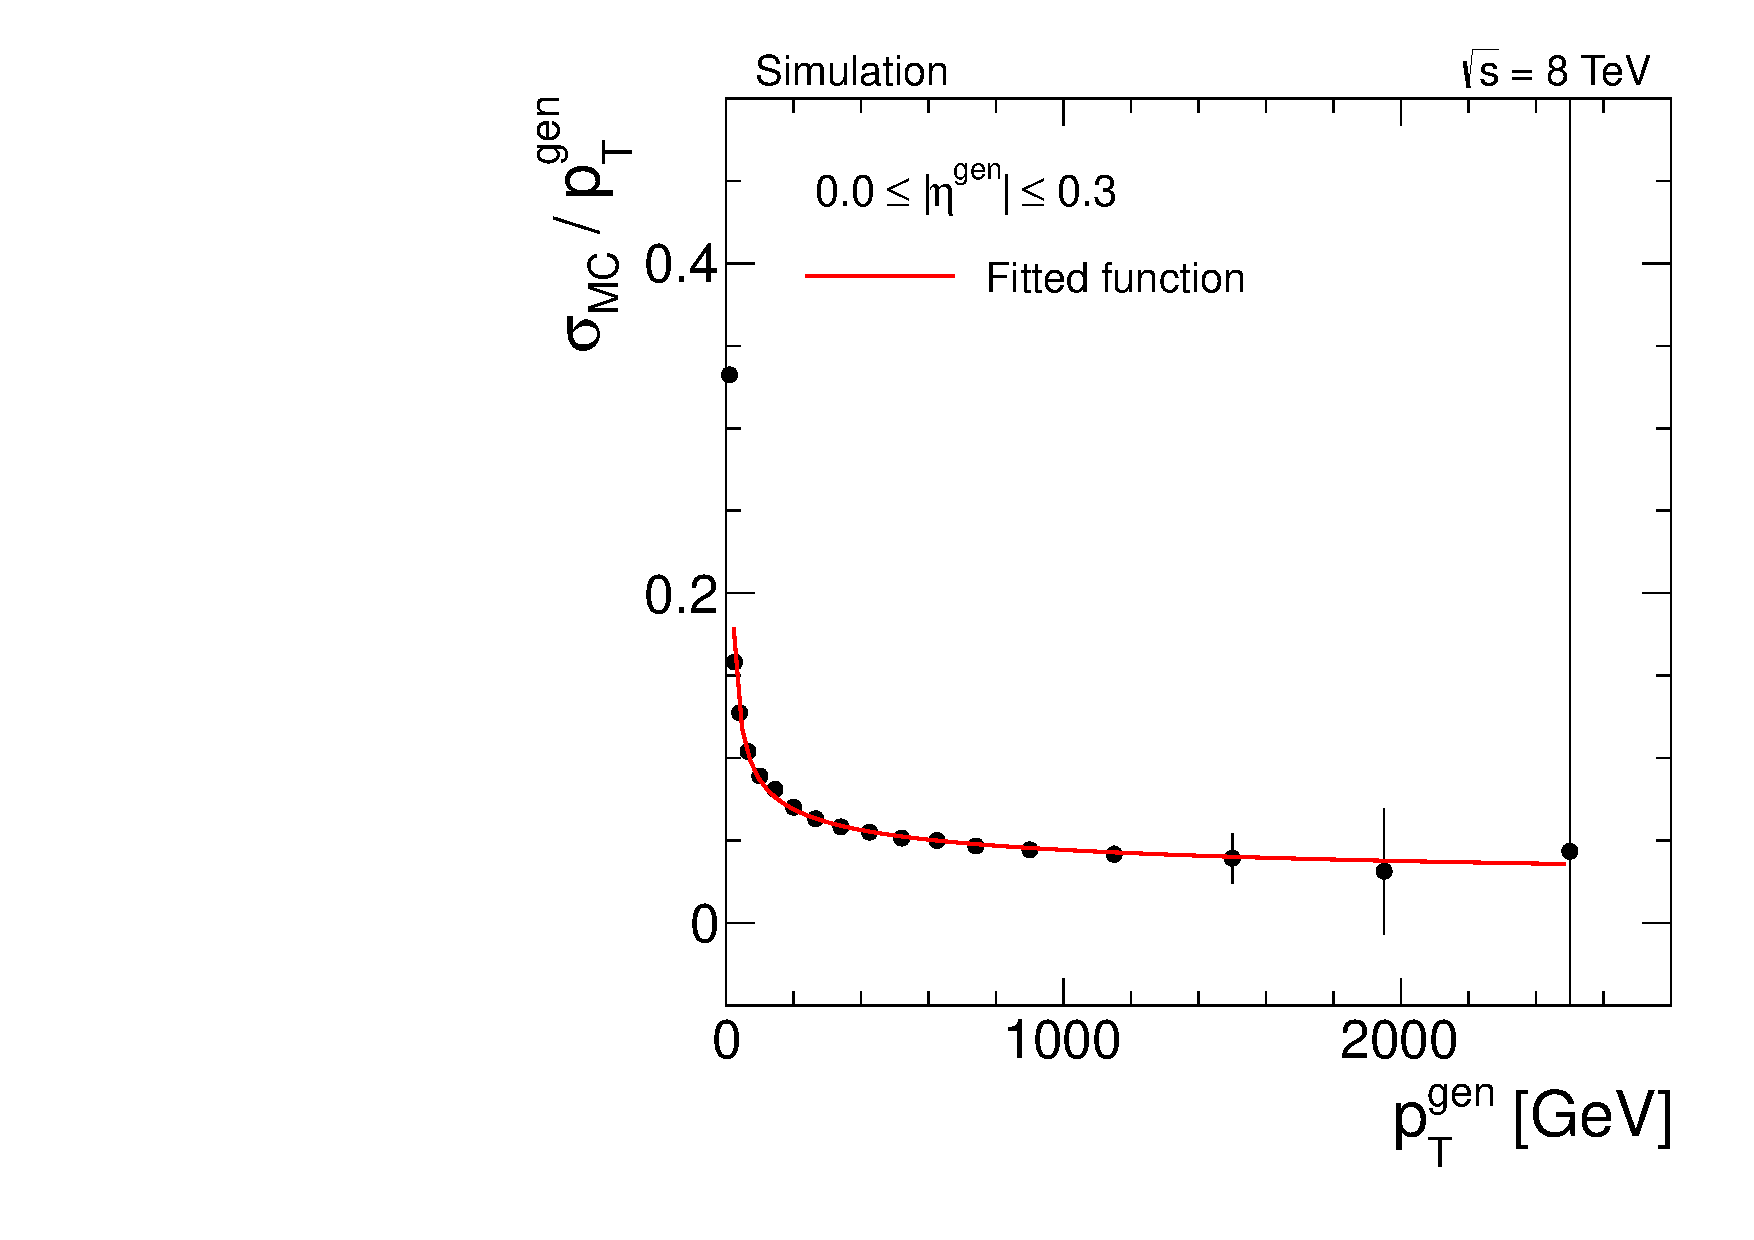
\includegraphics[width=0.49\textwidth]{figures/TruthRes_Eta0.pdf} &
                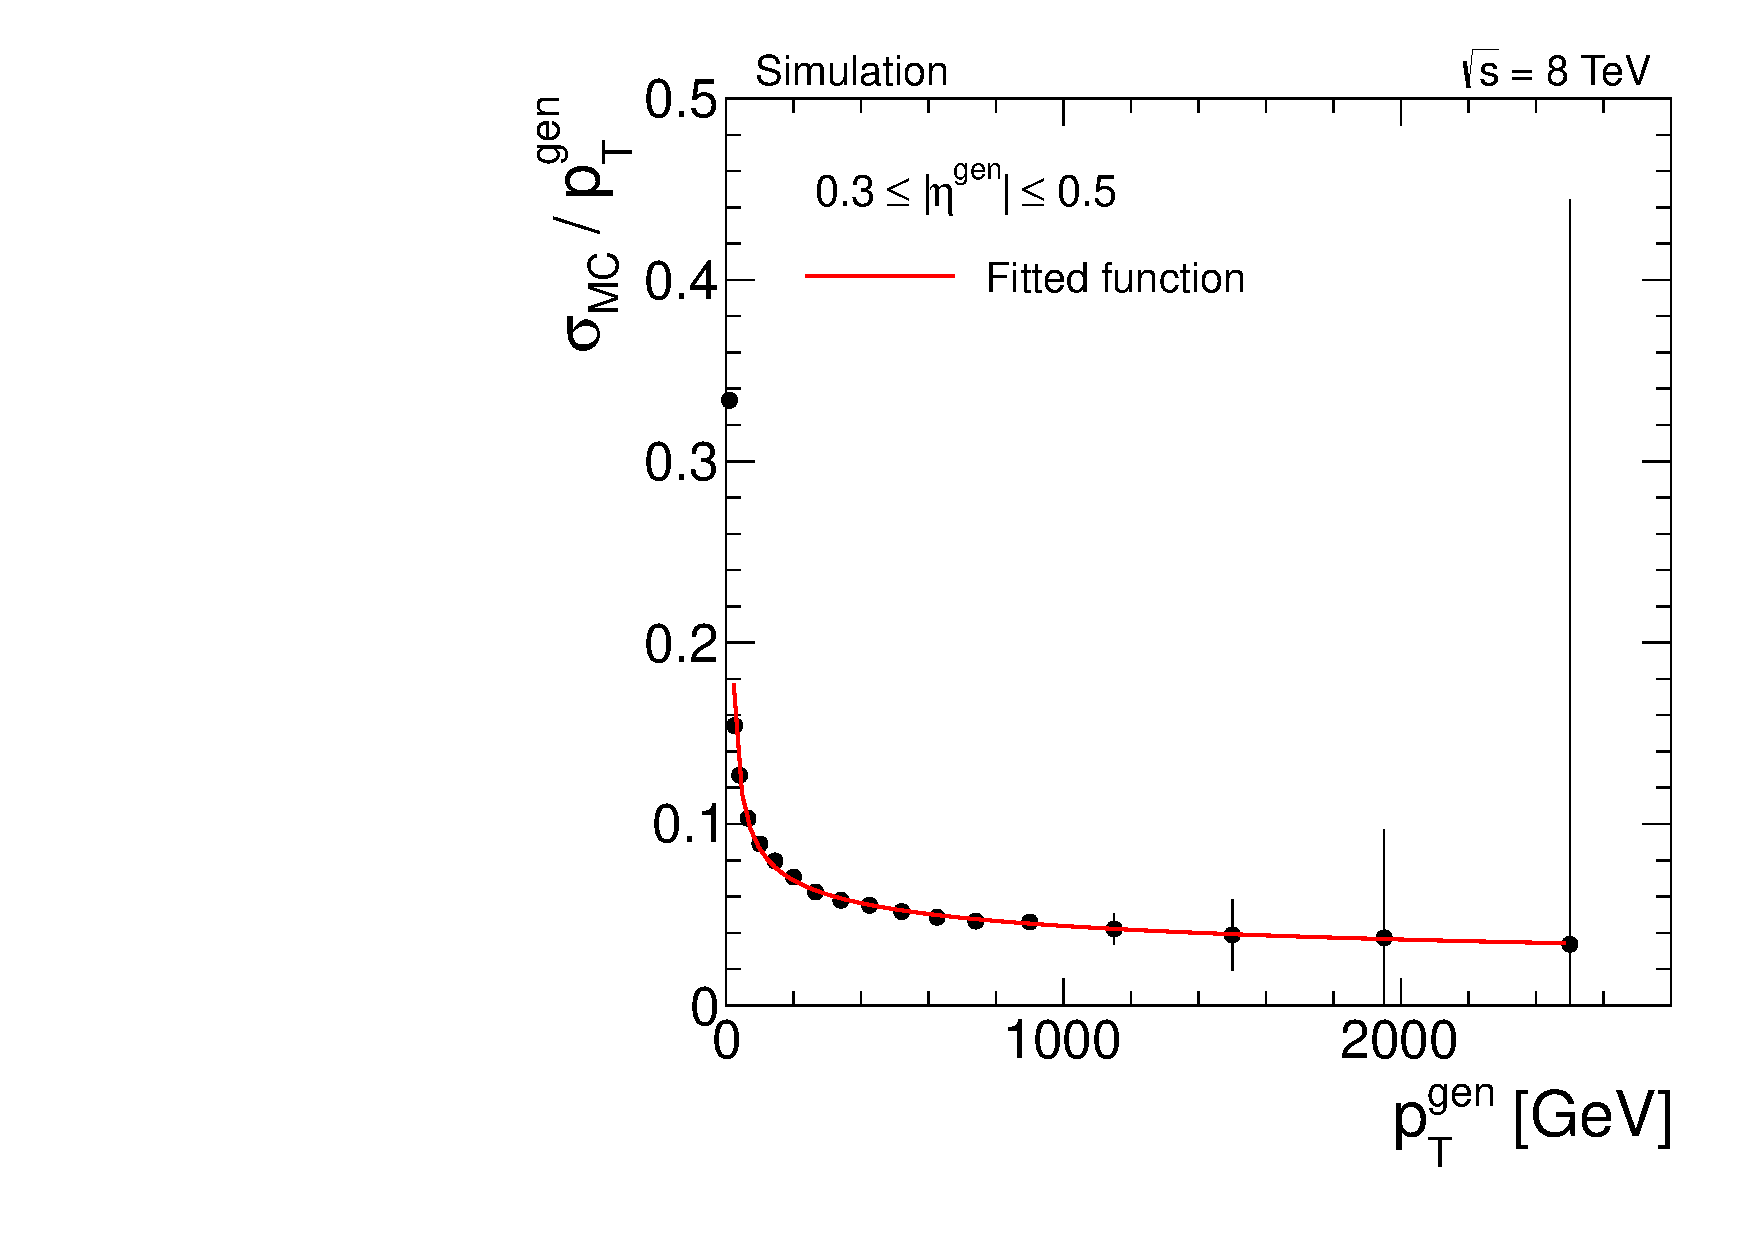
\includegraphics[width=0.49\textwidth]{figures/TruthRes_Eta1.pdf} 
  \end{tabular}
  \caption{Relative truth-\pt resolution derived from simulated events shown as a function of $\pt^\mathrm{gen}$. The distribution is fitted with a function as described in the next used as input for the kinematic fit employed to gain a balanced seed sample.}
  \label{fig:qcd_rs_truth_res}
\end{figure}
\\  
All events for which the fit converged within ($|\MHT^x| + |\MHT^y| < 0.02$) are then kept as seed events. Thus, the imbalance in each multijet event is removed by actually scaling the jet transverse momenta within the range of the respective resolution. Contributions to the seed sample from non-QCD multijet SM processes or even signal events in data do not have to be treated special, since this rebalancing procedure turns each of those events into QCD-like balanced topologies. Furthermore, the seed sample can be generated from an inclusive sample and their is no necessity to apply certain preselection cuts. Typically, selections suppressing high tails of missing energy tend to bias the QCD kinematics. This is due to the fact that for QCD events usually \HT and \MHT are correlated quantities, as high values of \MHT caused by severe jet mismeasurements can only occur, if there is a certain amount of energy in the event. Consequently, selection cuts removing high-\MHT tails also remove parts of the \HT spectrum resulting in an overall underestimation of QCD contributions to the high \HT and \MHT tails. Thus, the rebalancing with a kinematic fit allows to generate an unbiased seed sample.  

 \item \textbf{Response Smearing:}
The second step of the R+S method is made up of the smearing procedure. Here, all jets of a seed event are smeared with the full jet response distributions including non-Gaussian tails. This means that the magnitudes of the transverse momenta of the jets are scaled with a factor that is randomly obtained from the jet response distribution histogram of the respective $\pt$ and $|\eta|$ interval to model the reconstructed transverse momentum. These smeared events hence resemble the full QCD event kinematics and thus contributions from QCD events to the search regions can be estimated by imposing the respective selection cuts to the smeared events. \\
Similarly to the hadronic-tau background prediction, also the R+S method makes use of a bootstrap method. Instead of using all events only once, each seed event is smeared $N = 100$ times. The mean of these $N$ predictions is taken as final result while the statistical uncertainty is obtained as the standard deviation of this set of predictions. This definition of the statistical uncertainty on the prediction ignores the statistical fluctuations of the seed sample. However, since the seed sample is very large, this uncertainty is negligible to good approximation. \\
In order to validate the smearing procedure, generated QCD multijet events obtained from the \madgraph generator are smeared as described above and compared to fully simulated events at reconstruction level. This is performed on a sample which has a loose pre-selection at detetcor-level of $\NJets \ge 2$ and $\HT > 350$\gev applied. The result of this generator jet smearing is shown in Fig.~\ref{fig:qcd_rs_genjets}. 
\begin{figure}[!t]
  \centering

  \begin{minipage}[c]{1.\textwidth}
    \begin{center}
      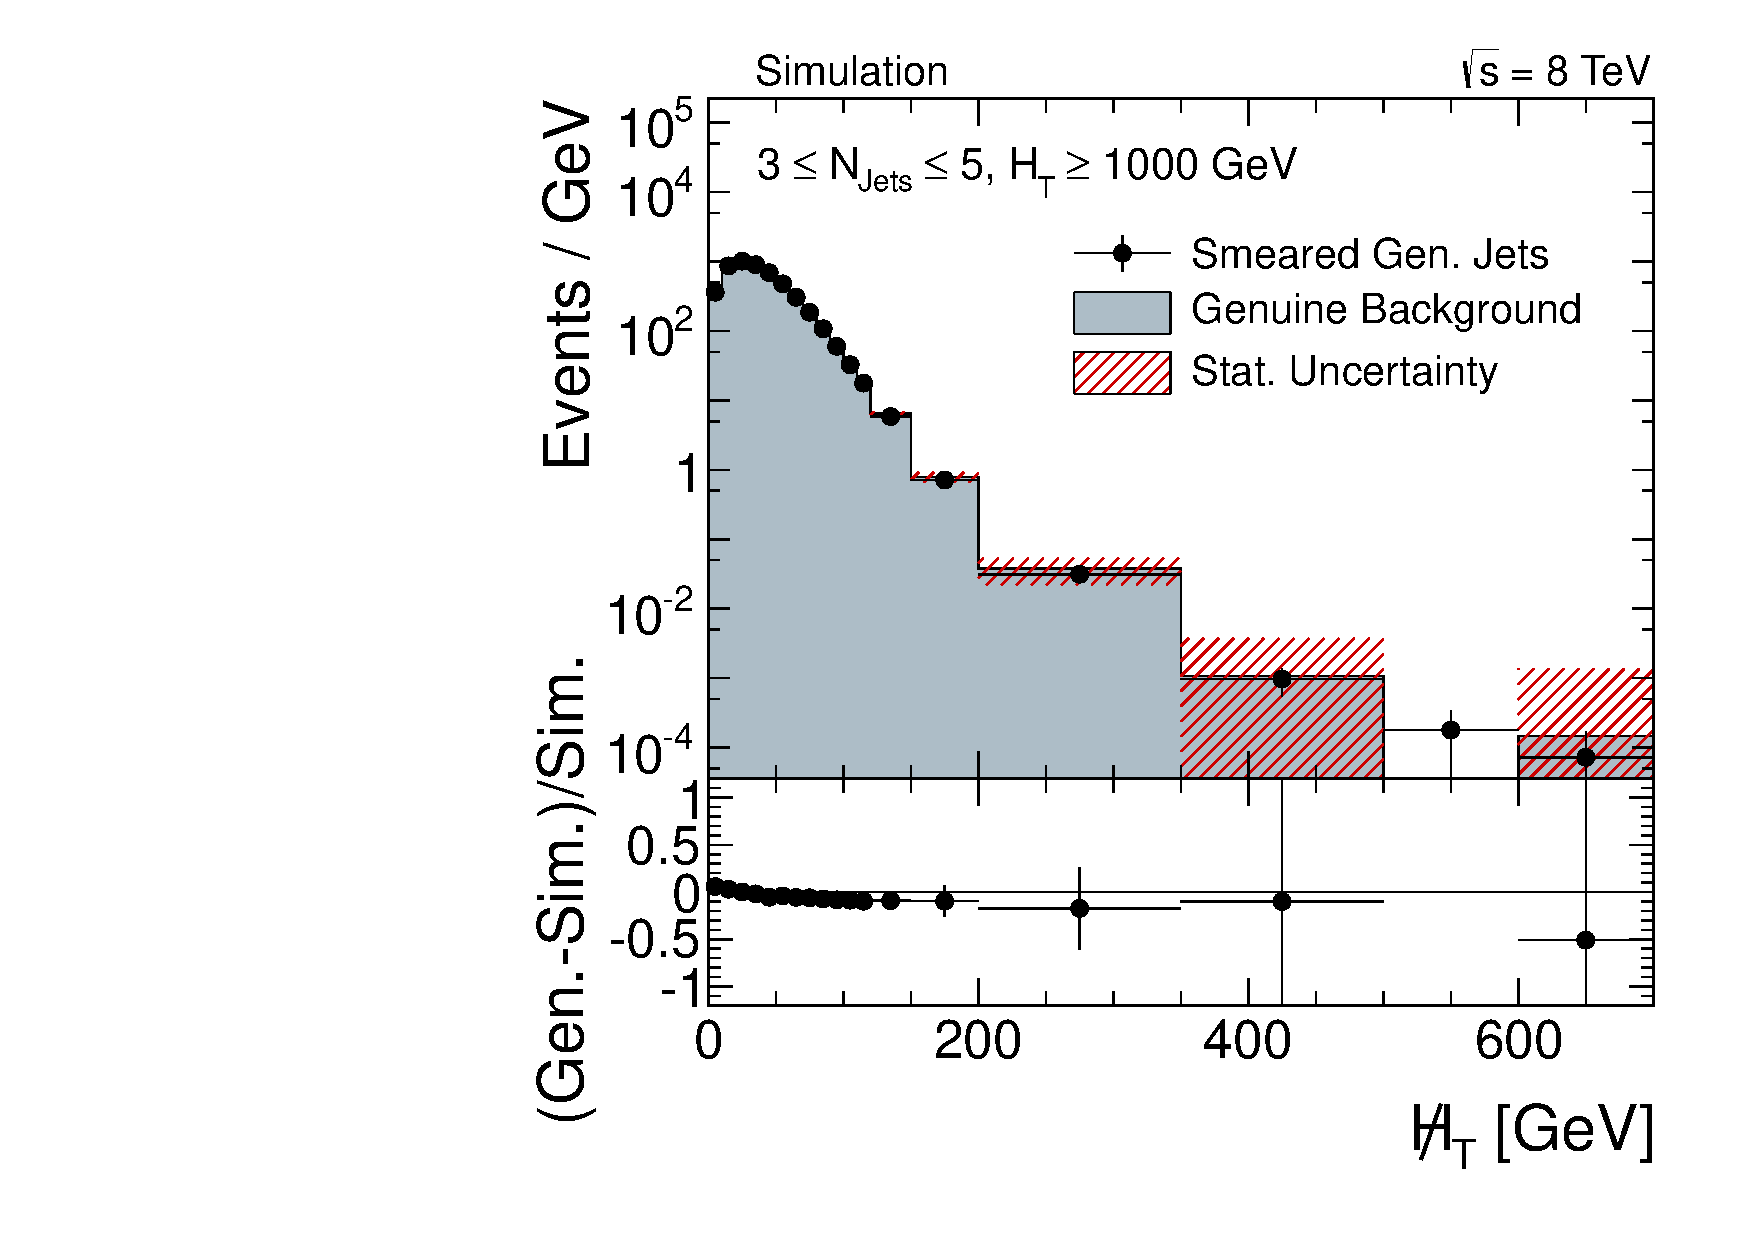
\includegraphics[width=0.49\textwidth]{figures/MHT_JetBin2_HThigh_madgraph_DR53X_chs_withoutPUReweighting_SmearedGenJets_v1.pdf}% \hspace {1.5 pt} 
      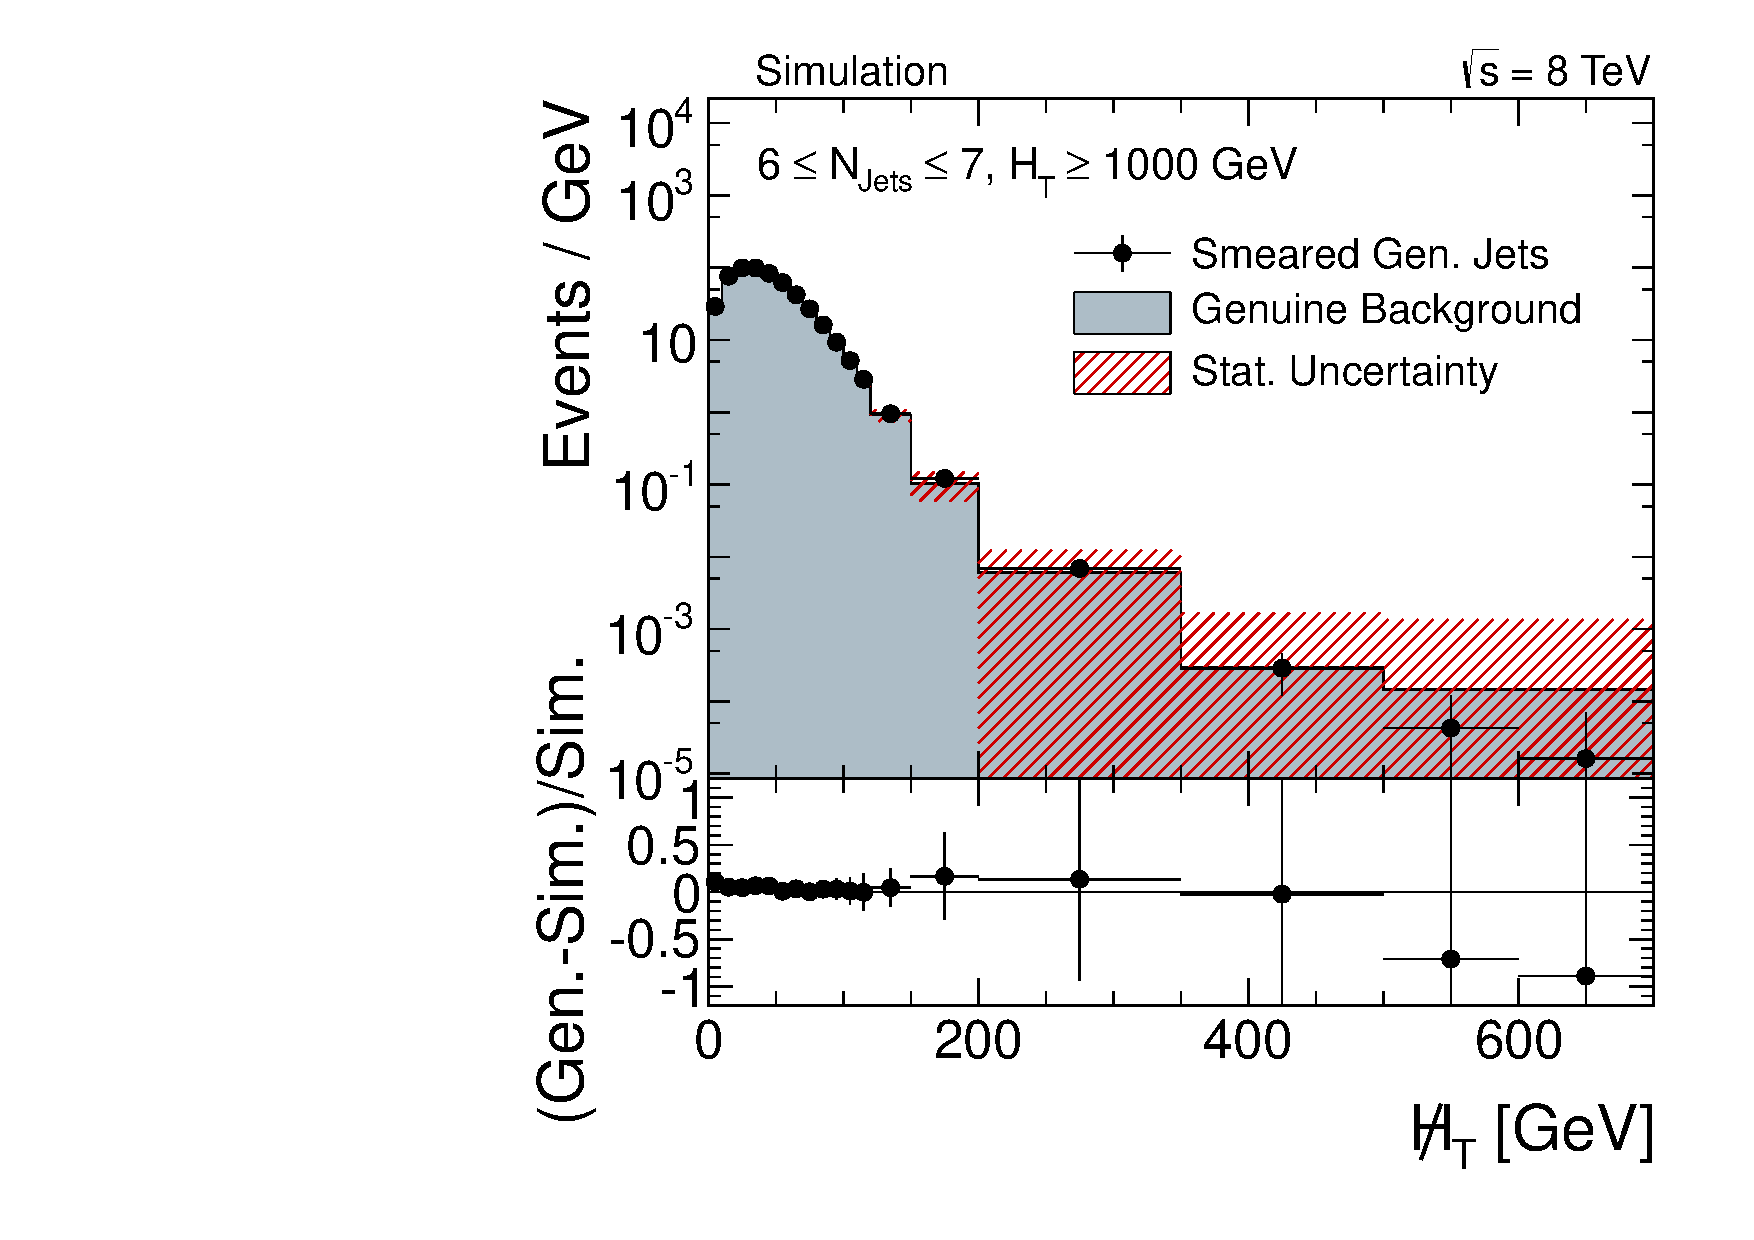
\includegraphics[width=0.49\textwidth]{figures/MHT_JetBin3_HThigh_madgraph_DR53X_chs_withoutPUReweighting_SmearedGenJets_v1.pdf}\\ 
      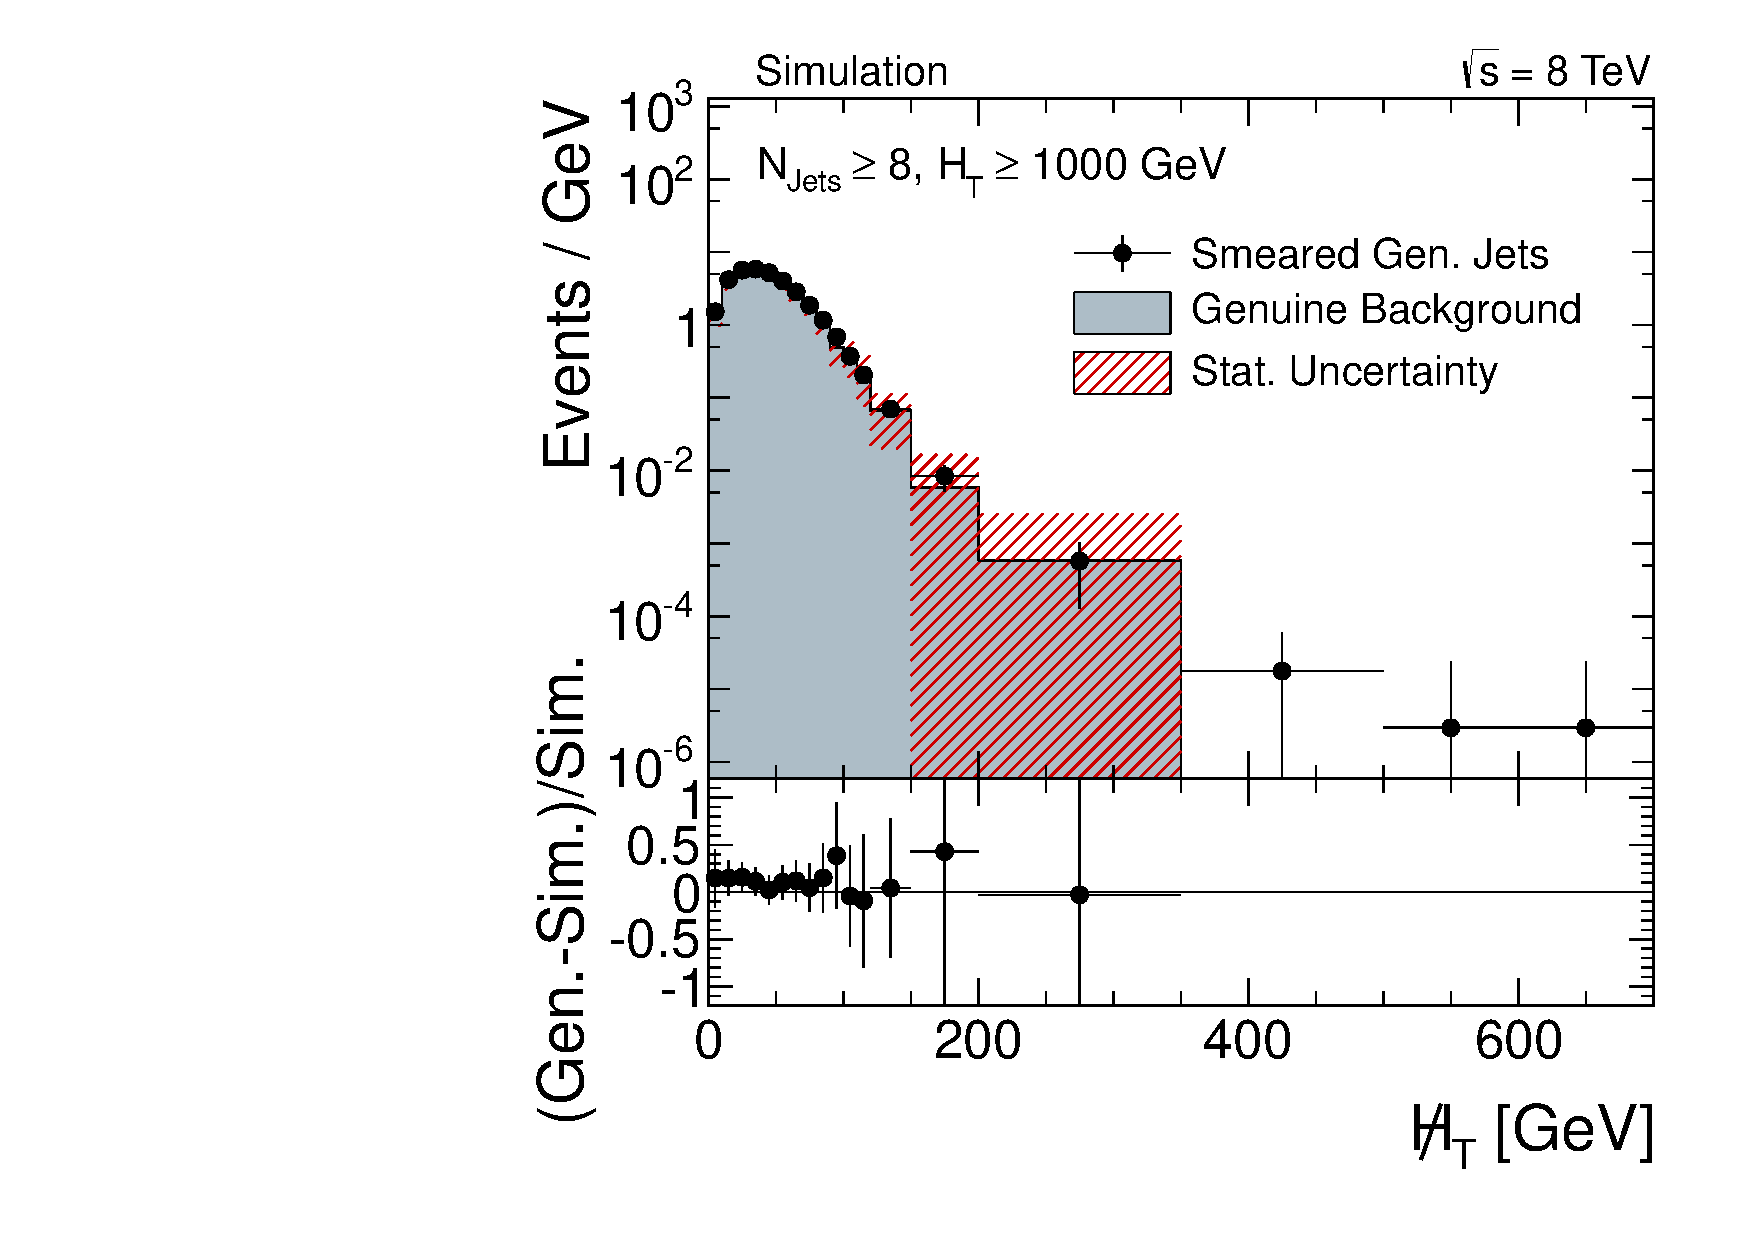
\includegraphics[width=0.49\textwidth]{figures/MHT_JetBin4_HThigh_madgraph_DR53X_chs_withoutPUReweighting_SmearedGenJets_v1.pdf}
    \end{center}
  \end{minipage}
  \caption{Generated jets obtained from a QCD multijet sample generated with \madgraph smeared with the truth response templates are compared to the expectation from full simulation. This comparison is shown for search regions with non-negligible QCD multijet background contributions as a function of \MHT defined by $\HT \ge 1000$\gev for $3 \le \NJets \le 5$ (\textit{top left}), $6 \le \NJets \le 7$ (\textit{top right}) and $8 \le \NJets$ (\textit{bottom}) after the application of the minimum $\Delta \phi$ selection.}
  \label{fig:qcd_rs_genjets}
\end{figure}
\\
Overall the distributions derived from the smeared generator jets reproduce nicely the expectation from the simulation. Potential disagreements between the predicted and expected quantities are in this thesis denoted \textit{non-closure} of the method and the respective tests of the agreement \textit{closure tests}. In general, non-closure can occur due to the limited granularity of the response template binning and the averaged flavour composition of the response. In the end, the non-closure of the method is quantified for the whole R+S method including also the rebalancing step (see Sec.~\ref{subsec:RPlusS_app}) and is assigned as systematic uncertainty to the QCD background prediction (see Sec.~\ref{subsec:RA2_syst_unc}). 
\end{description}
\begin{figure}[!t]
  \centering

  \begin{minipage}[c]{1.\textwidth}
    \begin{center}
      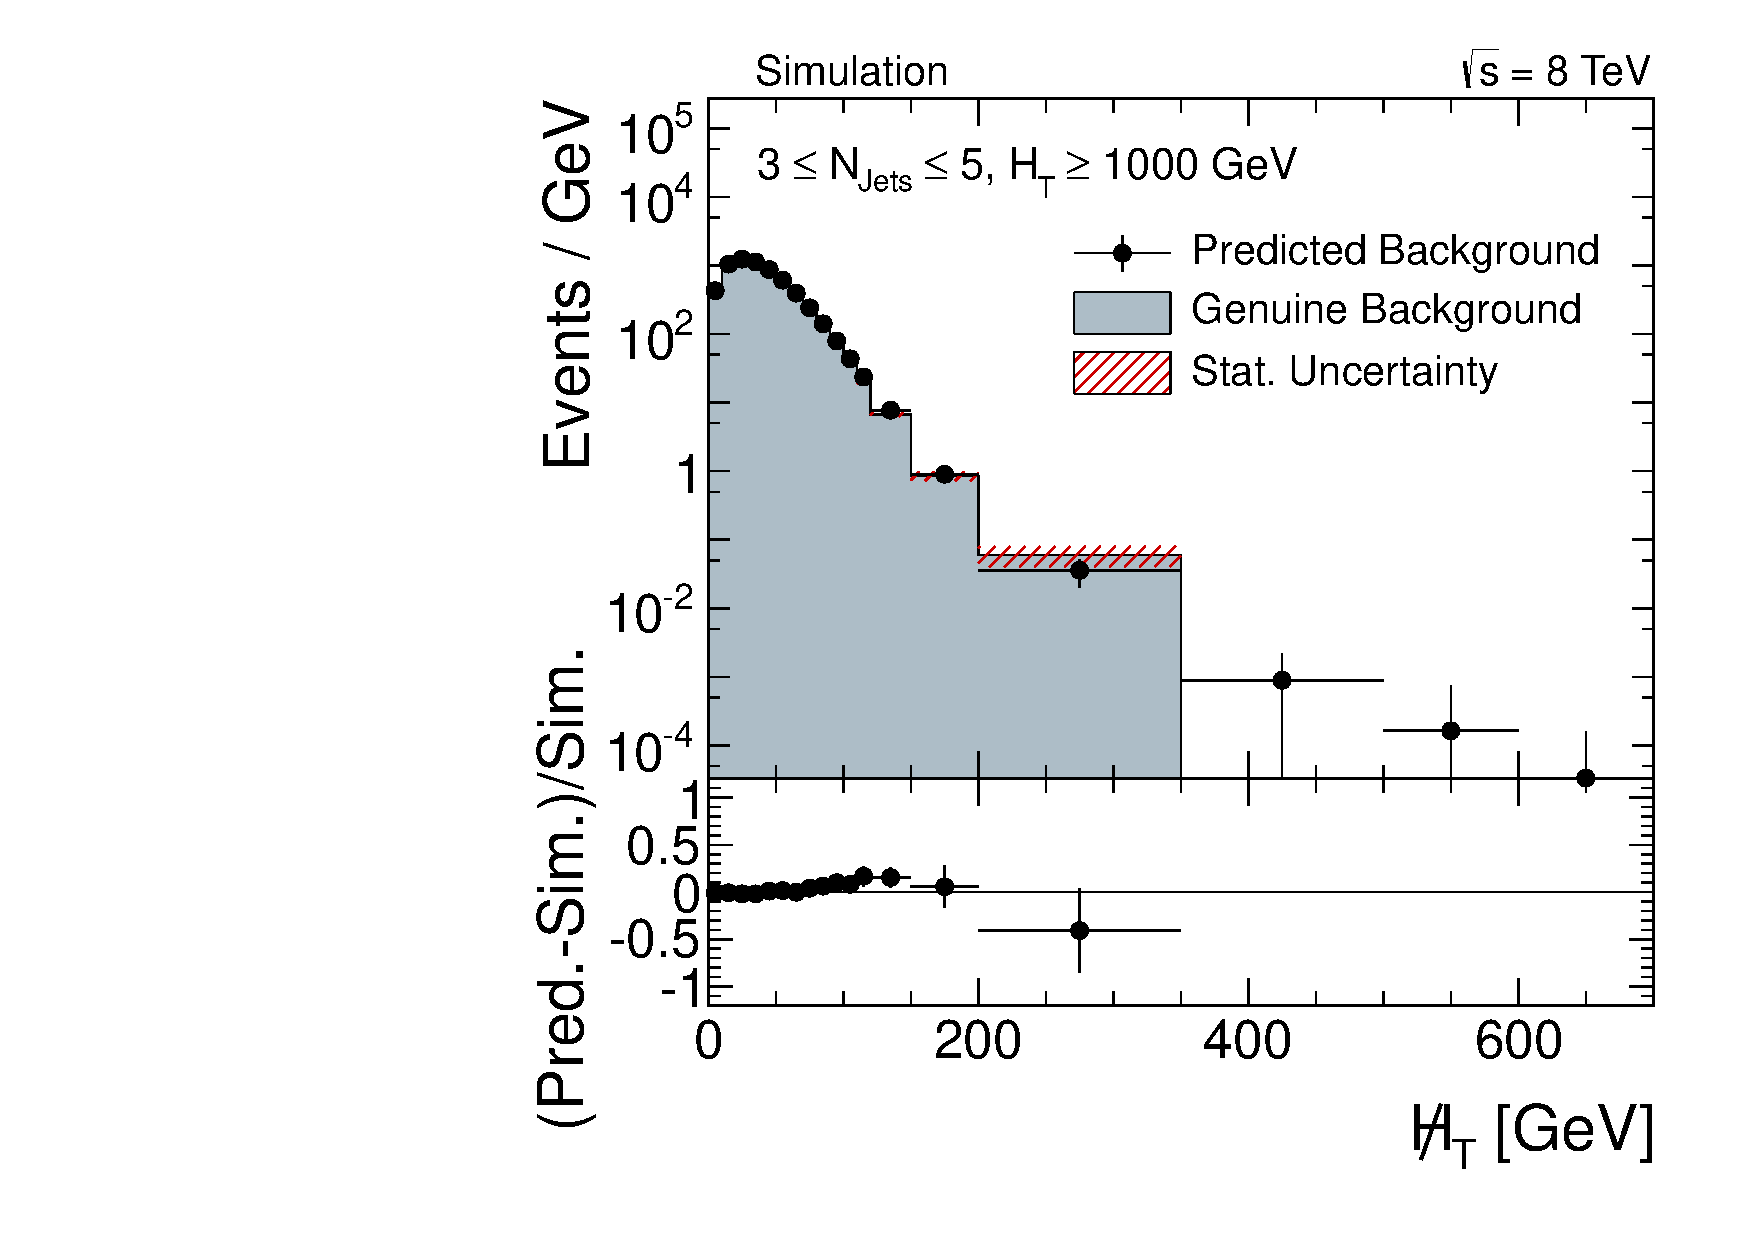
\includegraphics[width=0.49\textwidth]{figures/MHT_JetBin2_HThigh_pythia_chsJets_pt0_NoPU_v1.pdf}% \hspace {1.5 pt} 
      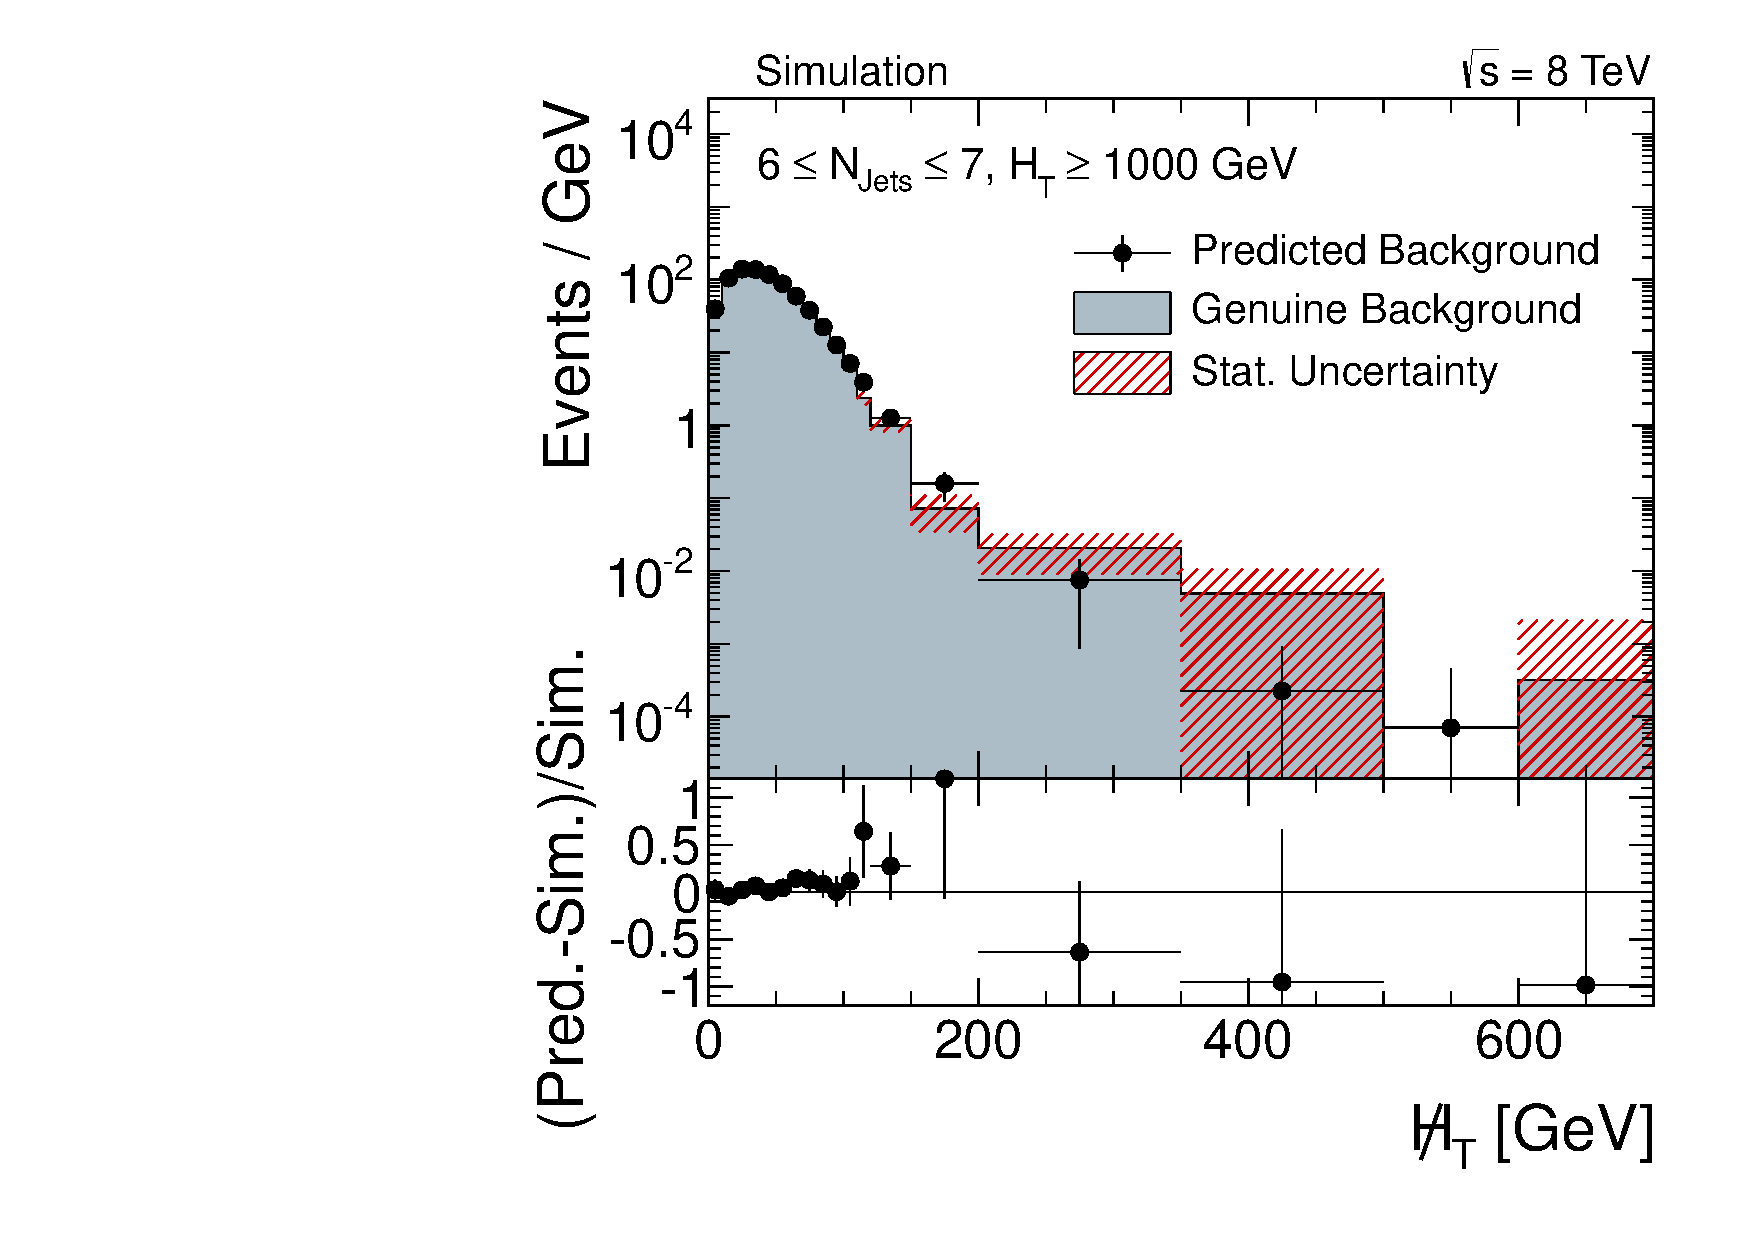
\includegraphics[width=0.49\textwidth]{figures/MHT_JetBin3_HThigh_pythia_chsJets_pt0_NoPU_v1.pdf}\\ 
      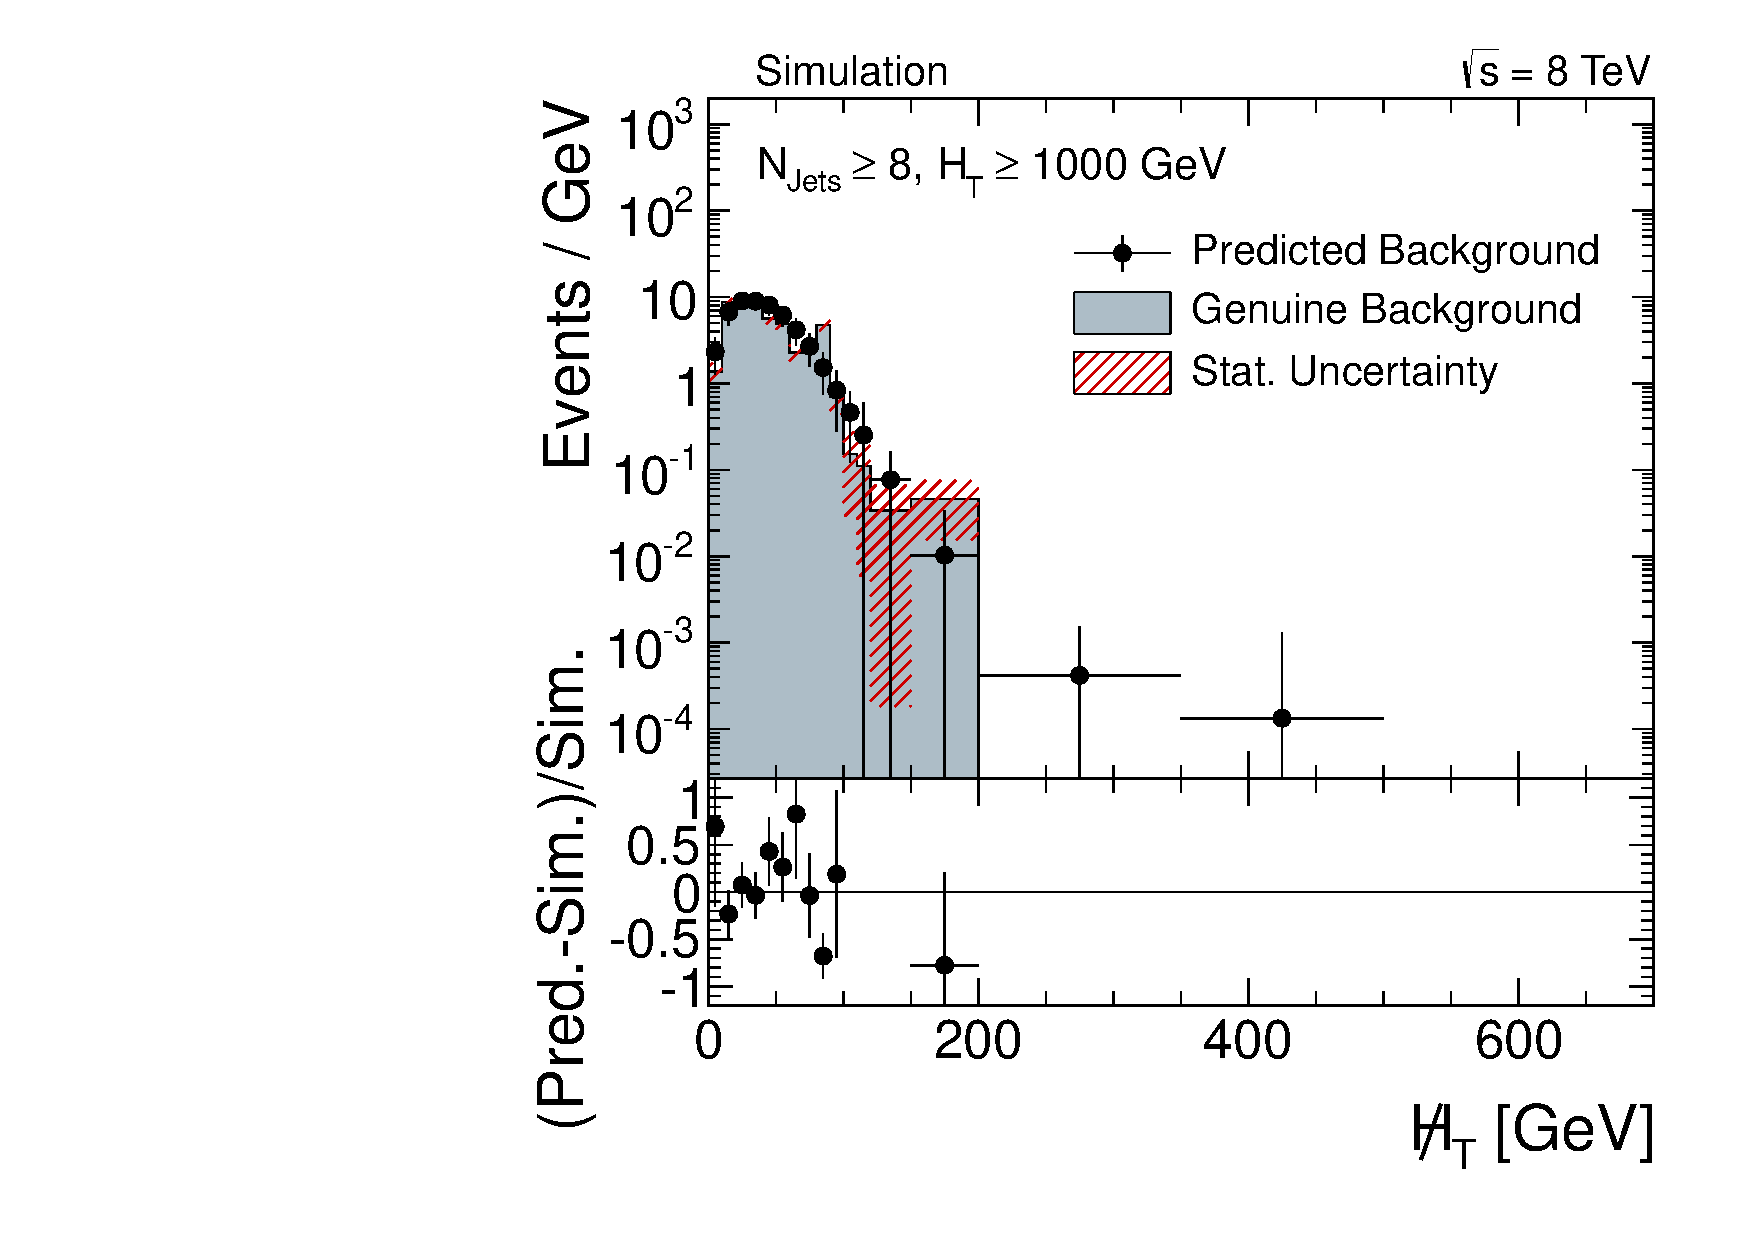
\includegraphics[width=0.49\textwidth]{figures/MHT_JetBin4_HThigh_pythia_chsJets_pt0_NoPU_v1.pdf}
    \end{center}
  \end{minipage}
  \caption{Prediction of QCD background on a QCD multijet sample generated with \pythia \textit{without the simulation of pileup events} compared to the expectation from full simulation. This comparison is shown for search regions with non-negligible QCD multijet background contributions as a function of \MHT defined by $\HT \ge 1000$\gev for $3 \le \NJets \le 5$ (\textit{top left}), $6 \le \NJets \le 7$ (\textit{top right}) and $8 \le \NJets$ (\textit{bottom}) after the application of the minimum $\Delta \phi$ selection.}
  \label{fig:qcd_rs_closure_nopu}
\end{figure}
In order to study the general feasibility of the R+S method to predict background contributions arising from QCD multijet events, the whole procedure is first performed on simulated QCD multijet events \textit{without} simulated pileup events and compared to the expectated event yields. Thus, the events are first reblanced with the kinematic fit adjusting the transverse momenta of all reconstructed jets in the event and then smeared according to the full jet response distribution, as done already for the smearing of generator jets. The resulting QCD background predictions are compared to the expectation in Fig.~\ref{fig:qcd_rs_closure_nopu} for representative search regions with non-negligible QCD background contributions. In general, the disagreement for the actual search regions of $\MHT > 200$\gev is statistically compatible with zero. Thus, the R+S method successfully predicts QCD multijet background in such idealised QCD multijet events without additional pileup interactions. The necessary adjustment of the method to realistic collision events is discussed in the next section.

\subsection{Application to Realistic Collision Events}
\label{subsec:RPlusS_app} 
The R+S method as introduced above has been shown to work properly on simulated events that contain no additional pileup events. However, in data several additional interactions per bunch crossing occur (cf. Sec.~\ref{sec:data}) which have to be taken into account in the R+S method as well. 
\begin{figure}[!t]
  \centering
  \begin{tabular}{cc}
                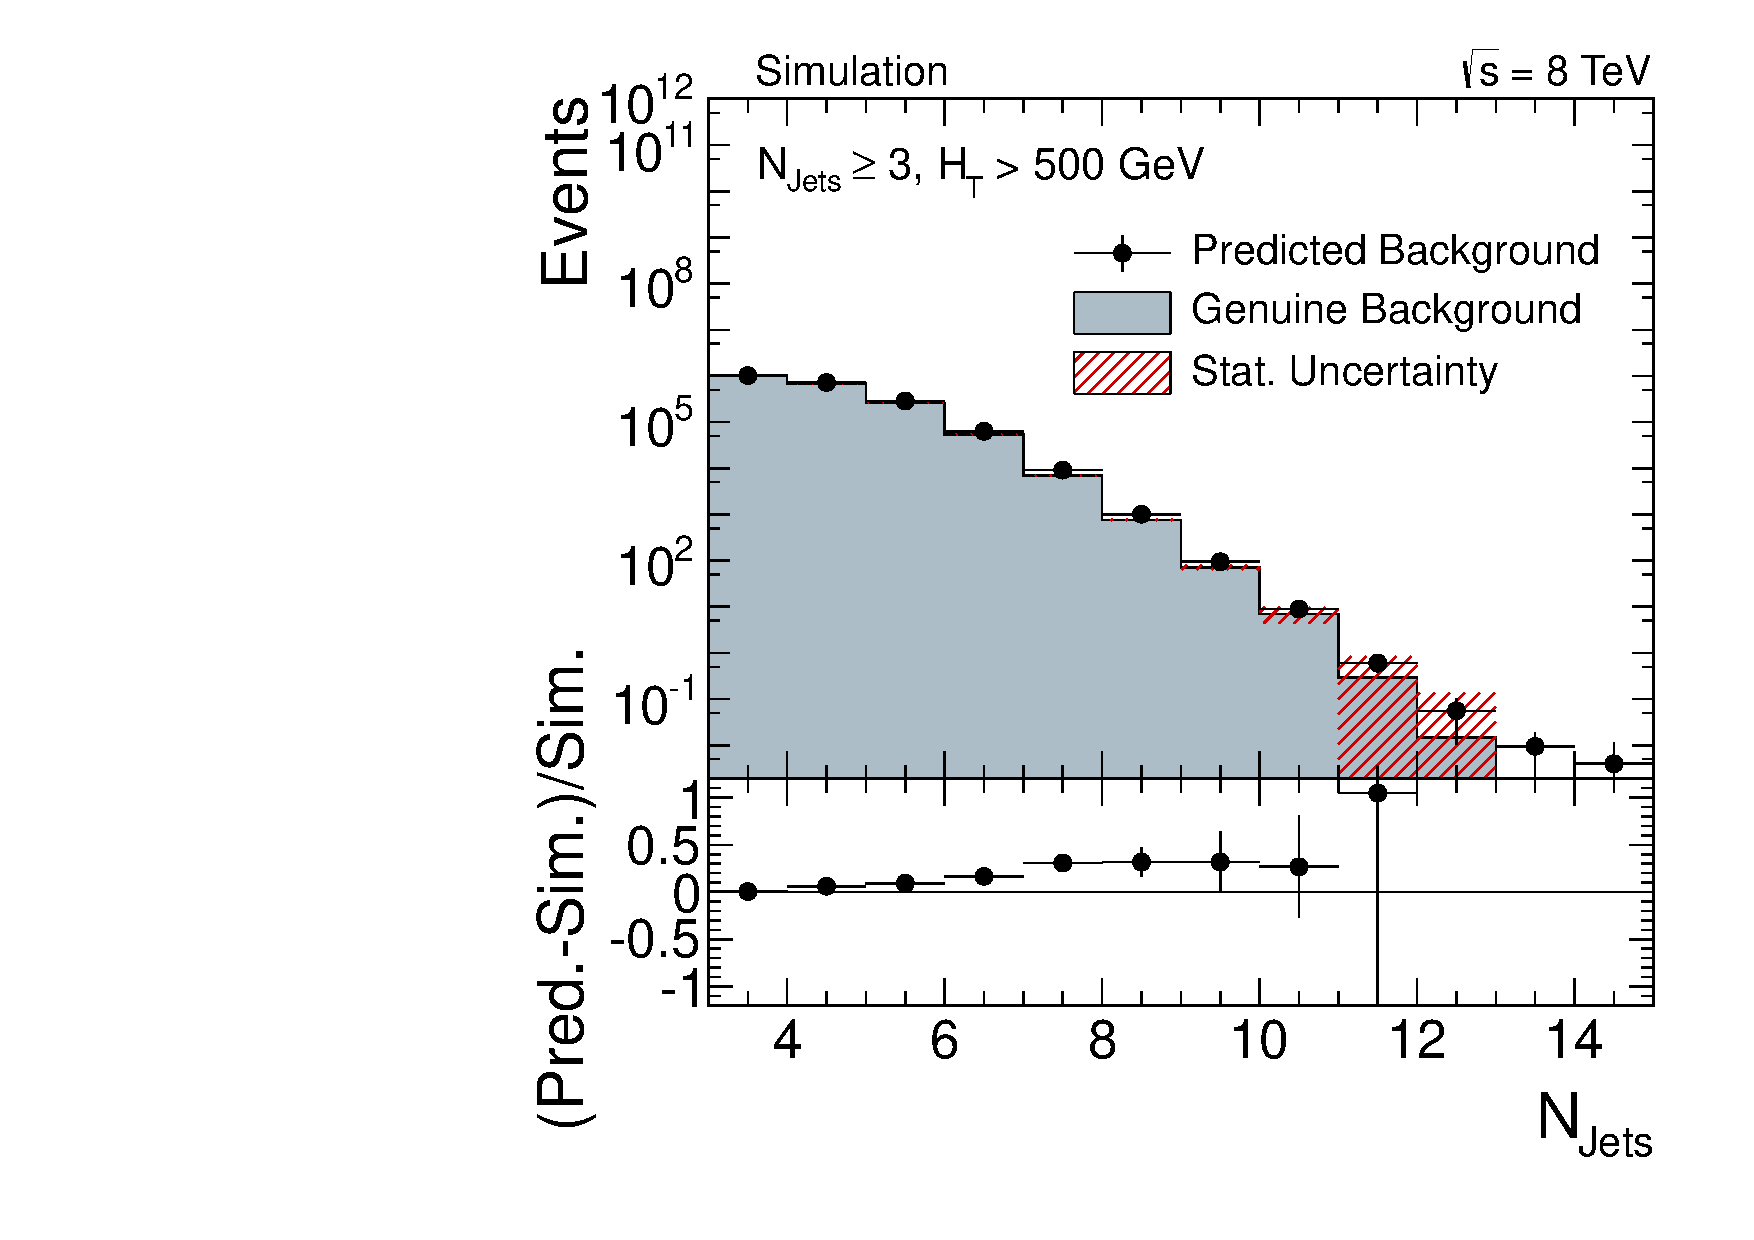
\includegraphics[width=0.49\textwidth]{figures/NJets_baseline_withoutMHT_madgraph_DR53X_chs_TuneZ2star_pt10_withoutPUReweighting_DoNotUseRebCorrection_v1.pdf} &
                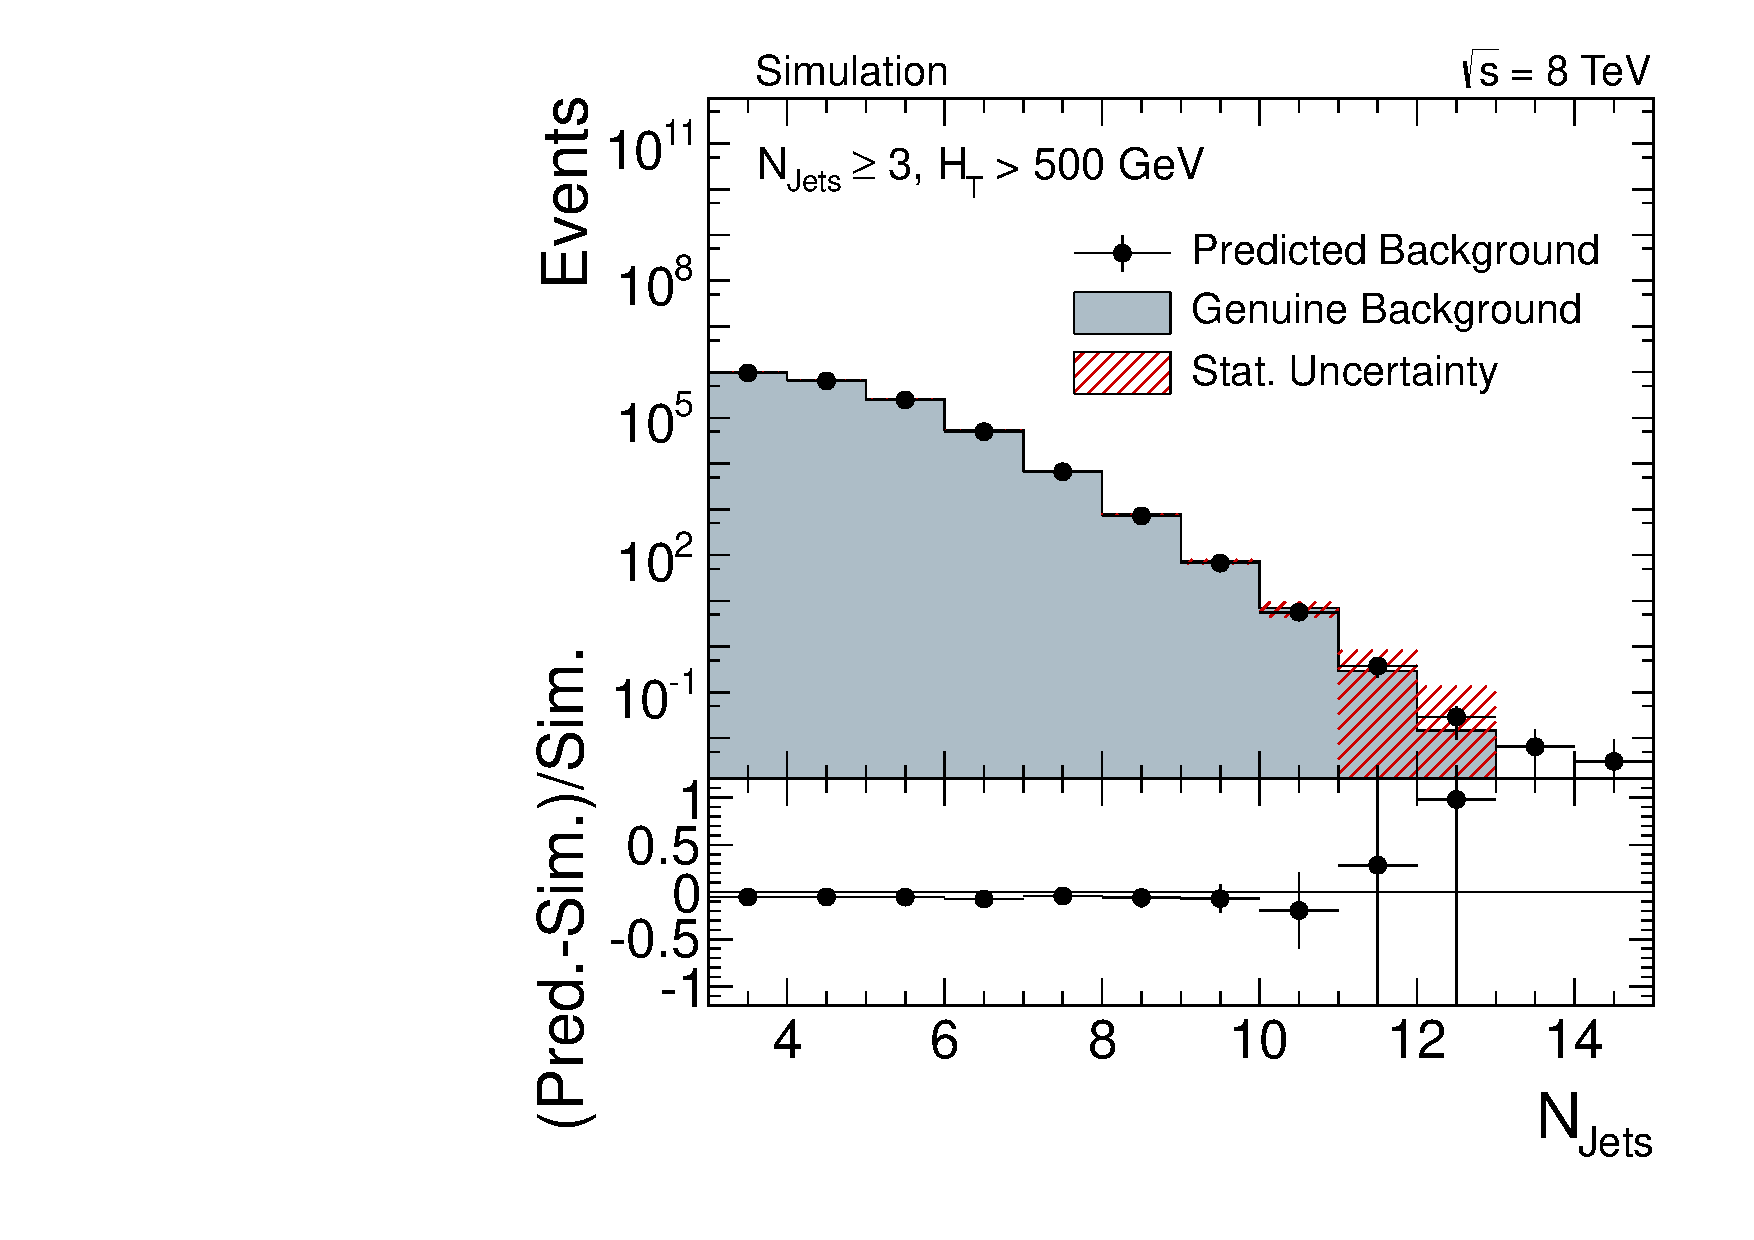
\includegraphics[width=0.49\textwidth]{figures/NJets_baseline_withoutMHT_madgraph_DR53X_chs_TuneZ2star_pt10_withoutPUReweighting_UseRebCorrection_v1.pdf} 

  \end{tabular}
  \caption{Prediction of QCD background on a QCD multijet sample generated with \madgraph compared to the expectation from full simulation showing the $N_{\text{jets}}$ distribution for a \pt cut of 10 GeV on jets considered in the rebalancing \textit{without} the application of a correction factor for the rebalancing (\textit{left}) and \textit{with} a correction of the rebalancing procedure (\textit{right}) as described in the text.}
  \label{fig:qcd_rs_rebnjets}
\end{figure}
\\
Jets assigned to an event, especially soft jets, do not necessarily have to belong to the hard interaction, but might arise from pileup events. Thus, it is necessary to discard jets below a certain \pt threshold in the rebalancing step in order to not balance pileup jets against the hard process. This \pt threshold can for instance be chosen such that a good inclusive closure of the method in simulated events is observed. Nevertheless, by not taking all jets into account in the rebalancing, also soft jets belonging to the hard interaction are not considered. By doing this, additional imbalance in the event is introduced. It can be observed that this affects the kinematic fit such that especially jets with small \pt ($<$ 100 GeV) are on average rebalanced to too high momenta. This results in the observation that more jets pass the threshold of 50\gev to be counted for \NJets than expected. As a consequence, the number of predicted QCD events in the higher jet multiplicity bins is too large. The resulting trend in the \NJets distribution is illustrated in Fig.~\ref{fig:qcd_rs_rebnjets} (left). Here, only jets with \pt$> 10$\gev are considered for the rebalancing procedure.
\begin{figure}[!t]
  \centering
  \begin{tabular}{cc}
                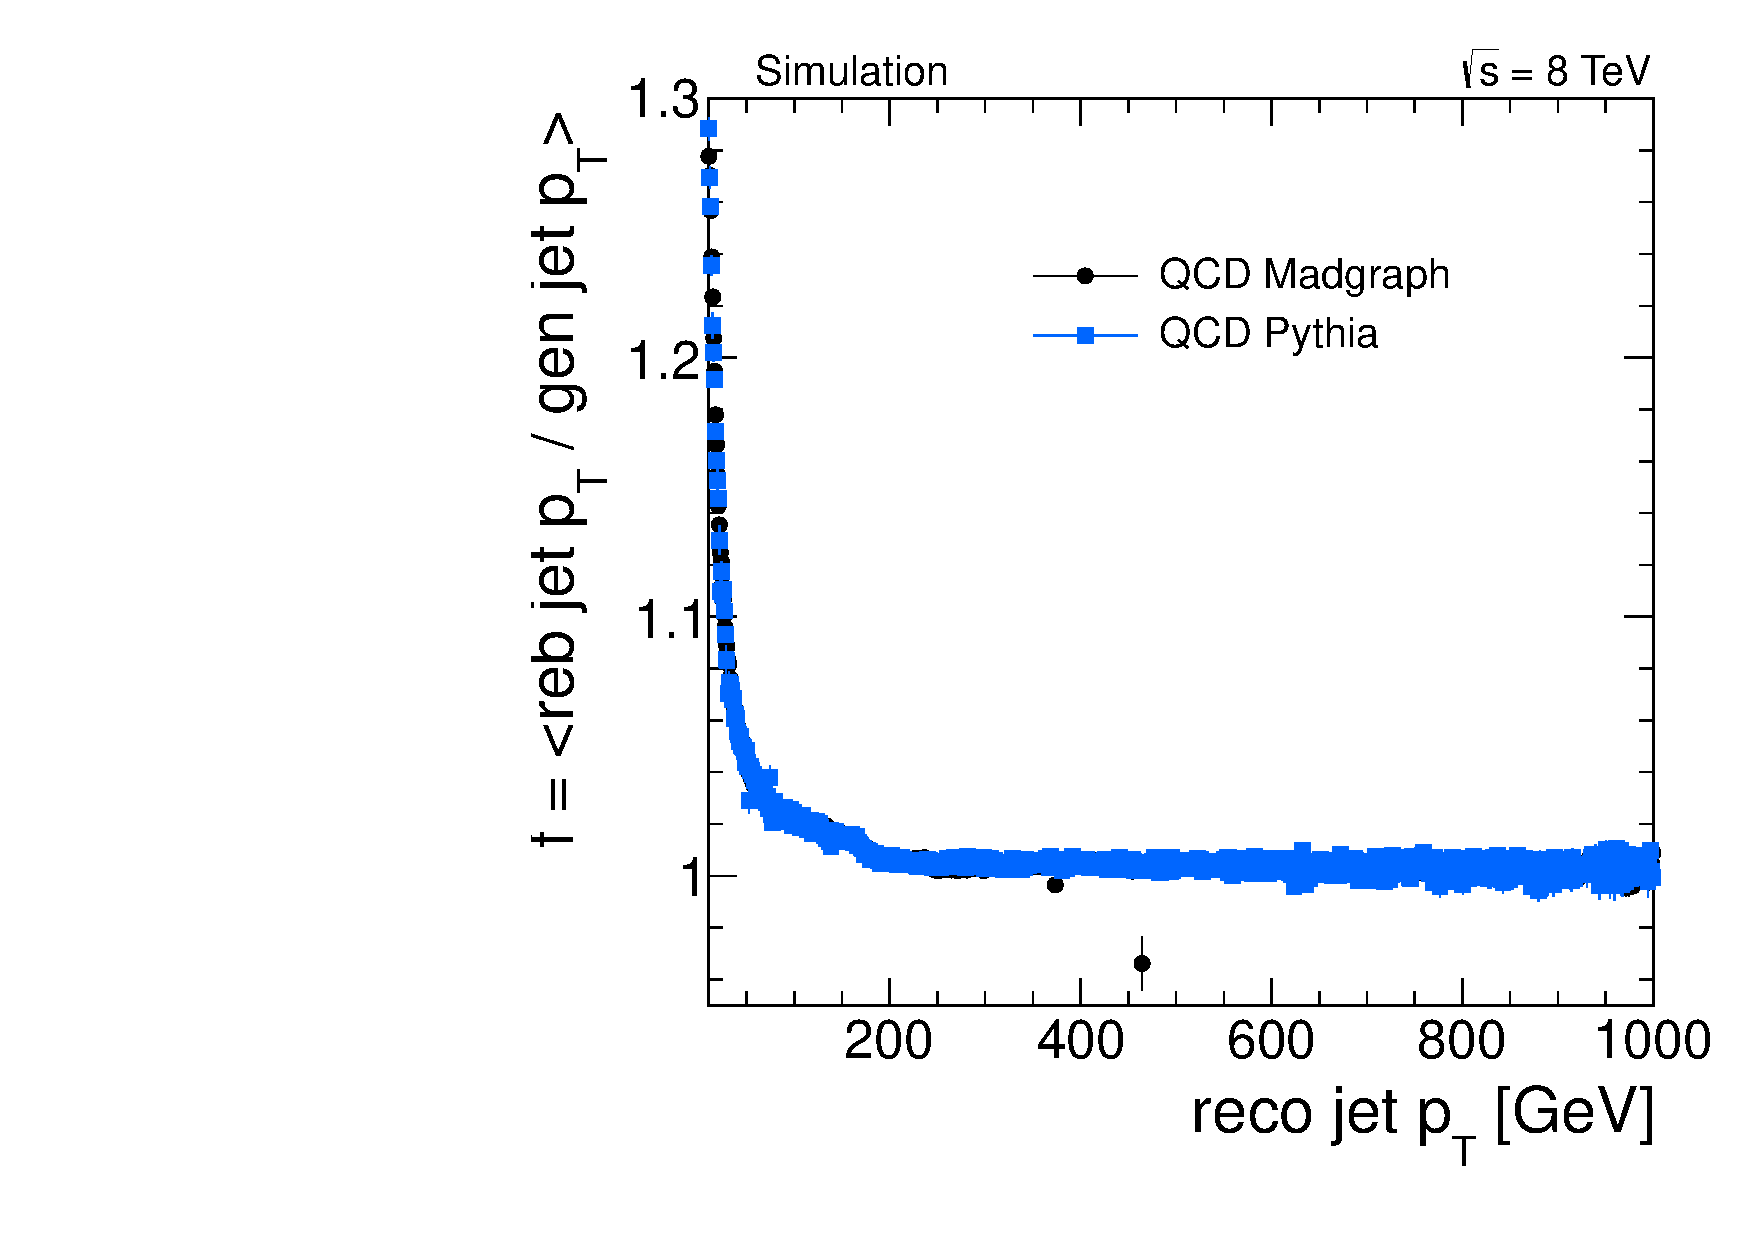
\includegraphics[width=0.49\textwidth]{figures/RebalanceCorrectionFactors_DR53X_chsJets_TuneZ2star_withoutPUReweighting_pt10_vsRecoWithMadgraphComp.pdf} &
                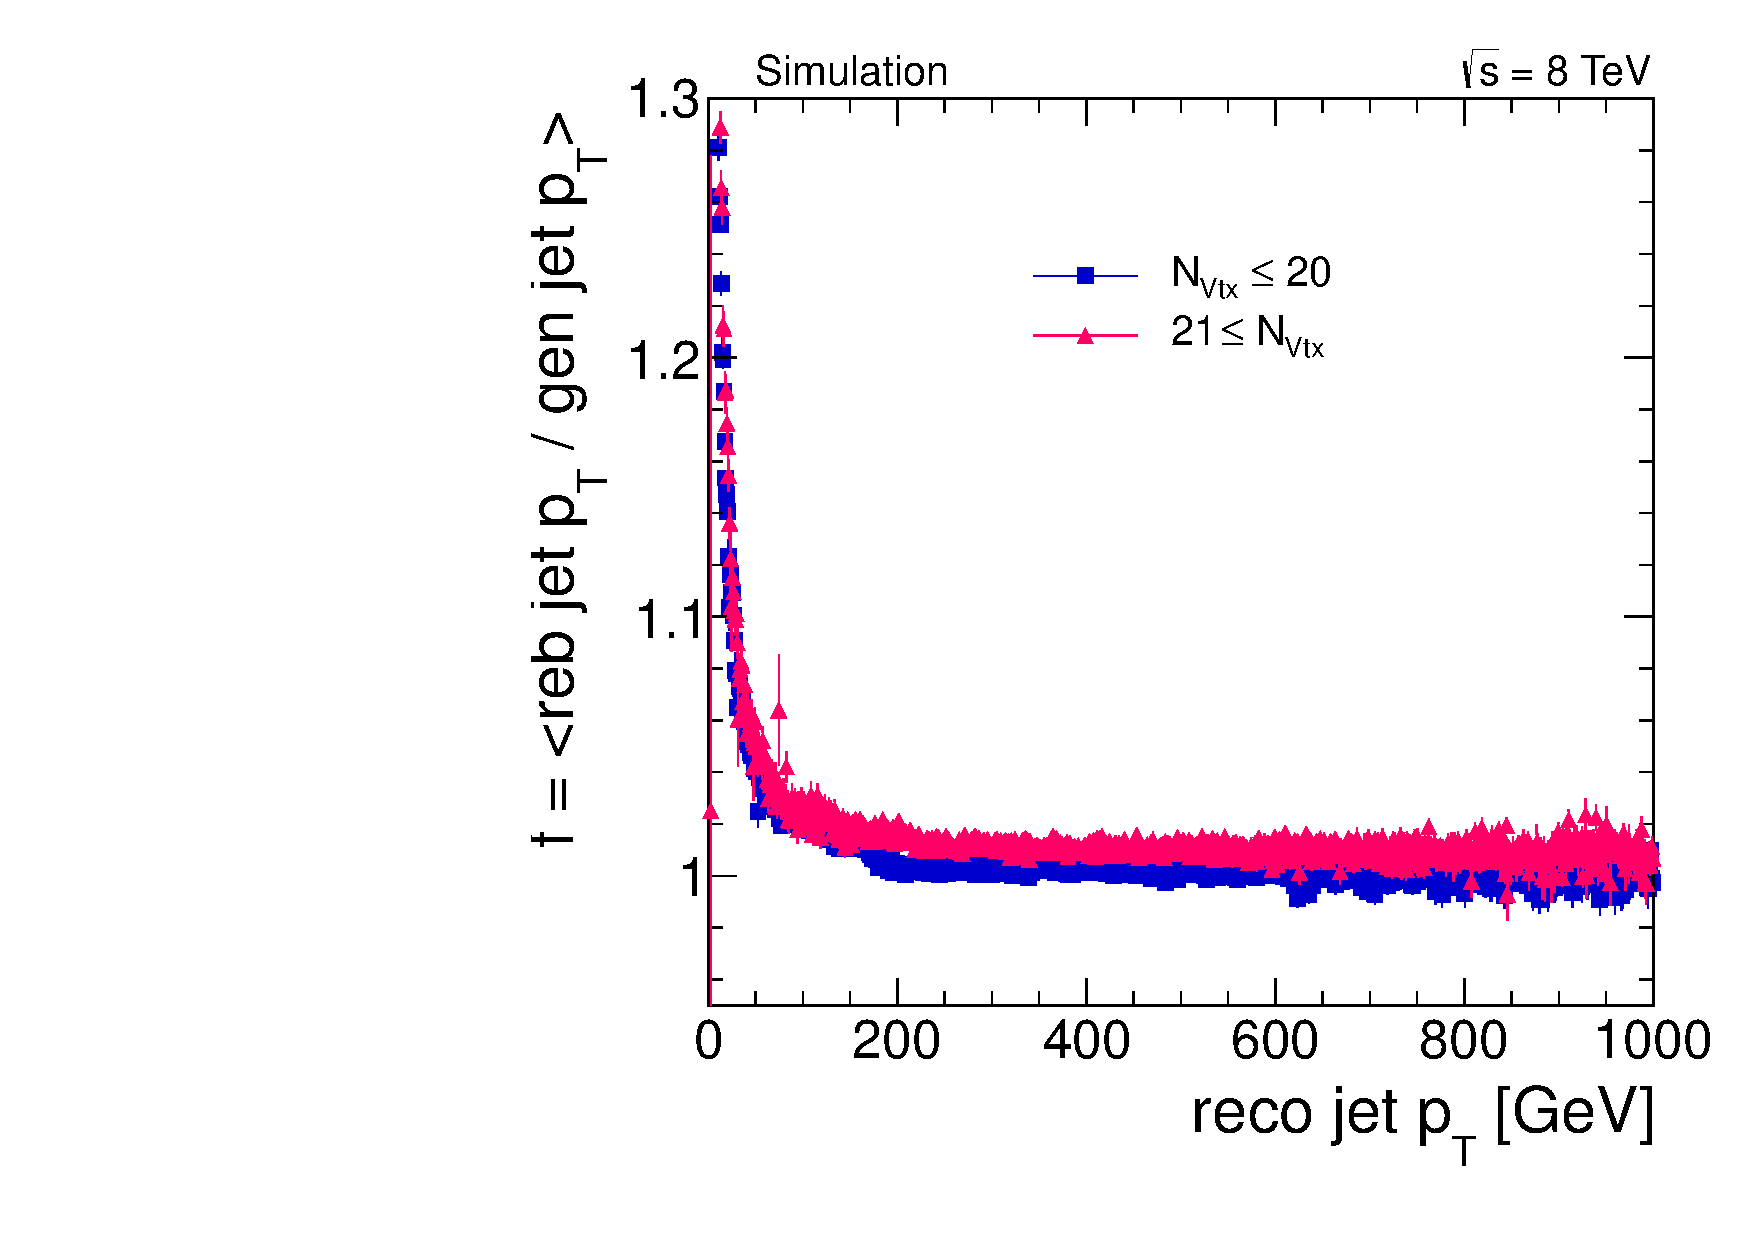
\includegraphics[width=0.49\textwidth]{figures/RebalanceCorrectionFactors_DR53X_chsJets_TuneZ2star_withoutPUReweighting_pt10_vsRecoNVtxSplit.pdf}\\

  \end{tabular}
  \caption{Comparison of the rebalance correction factor determined on the \pythia and the \madgraph QCD Monte Carlo (left) and rebalance correction factor for different primary vertex bins (right).}
  \label{fig:qcd_rs_rebfactor}
\end{figure}
\\
In order to account for this unavoidable threshold effect, an empirical correction factor (f) is introduced. This is done by comparing the \pt-spectrum of the rebalanced jets to the \pt-spectrum of matched generated jets after the rebalancing step in which jets below 10\gev have been excluded from the rebalancing procedure. The mean of this ratio for all events is taken as correction factor and evaluated versus the momentum of the matched reconstructed jets. The correction factor is employed such that in the rebalancing procedure each jet momentum is scaled by $1/\rm{f}$ before the kinematic fit is performed. Thus, the effect of overpredicting the jet momenta of jets with small transverse momenta is taken care of by downscaling the jet momenta before the kinematic fit by a factor representing the average overprediction. This adjusted method then leads to correct predictions of the QCD event yields also in the high jet multiplicity bins as demonstrated in the right plot of Fig.~\ref{fig:qcd_rs_rebnjets}.\\
The correction factor is derived by using generator-truth information and hence can only be determined on simulated event samples. However, this can be done for different samples to study, if the correction is somewhat generator dependent. The rebalance correction factor is thus derived for the QCD multijet samples obtained from \pythia and \madgraph. The difference of the correction factors derived from these two samples is found to be of the order of $1-2\%$ cf. Fig.~\ref{fig:qcd_rs_rebfactor} (left). In addition, the correction factor was also determined for different bins of primary vertices and thus for different pile-up conditions. It is observed that the functional form of the correction factor is independent of the pile-up conditions cf. Fig.~\ref{fig:qcd_rs_rebfactor} (right). This justifies the assumption that the observed harder jet \pt-spectrum after the rebalancing step without the application of correction factor is due to the acceptance of the jet \pt cut on the jets considered for the rebalancing. Therefore, the correction factor derived from simulation is applied to data where the same \pt cut value of 10\gev for jets considered in the rebalancing is chosen. 

\subsection{Validation in Simulated Events}
\label{subsec:validation_mc}
The quality of the R+S method to predict background contributions from QCD multijet events is tested on simulated samples by several closure tests in different kinematic regions. Therefore, the data-based prediction is applied to simulated events and compared to the results from full simulation, as explained in Sec.~\ref{subsec:RPlusS_app}. The different closure tests as function of \MHT for various jet multiplicity bins for a low \HT ($= 500 - 1000$~GeV) and a high \HT ($\ge 1000$~GeV) selection are shown in Fig.~\ref{fig:qcd_rs_closure} for simulated events obtained from \madgraph. In general, the prediction shows a good agreement with the expected QCD background contributions. Especially, for the high \HT regions, where QCD background is even more important than for lower \HT values, the agreement is reasonable. However, deviations between prediction and expectation occur, which have to be considered as remaining bias of the R+S method and treated as systematic uncertainty. Due to the limited statistics of the simulated sample, the bias uncertainty is not evaluated for each search region individually, but for the different jet multiplicity intervals and a low and a high \HT selection, corresponding to the kinematic regions defined in Fig.~\ref{fig:qcd_rs_closure}.
\begin{figure}[!hp]
  \centering
  \begin{tabular}{cc}
                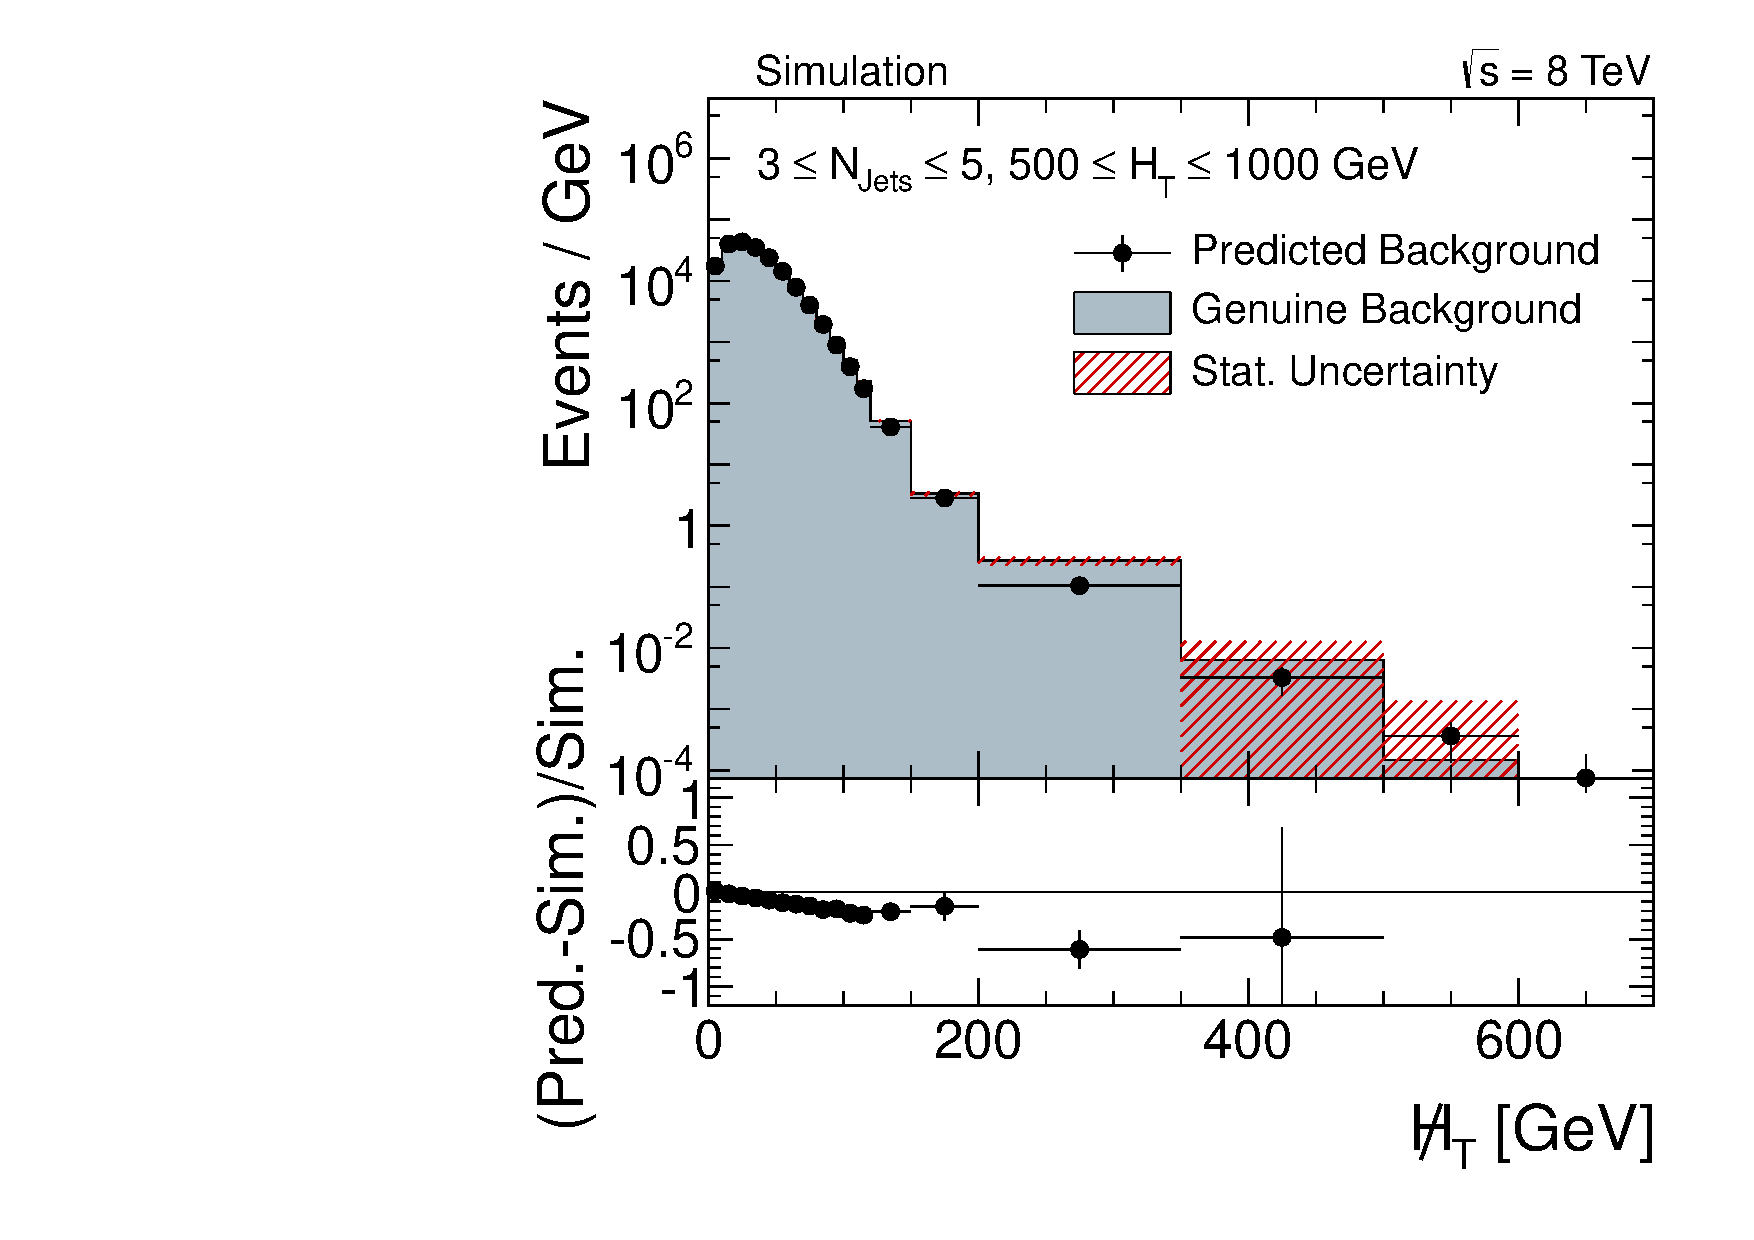
\includegraphics[width=0.49\textwidth]{figures/MHT_JetBin2_HTlow_madgraph_DR53X_chs_TuneZ2star_pt10_withoutPUReweighting_UseRebCorrection_v1.pdf} &
                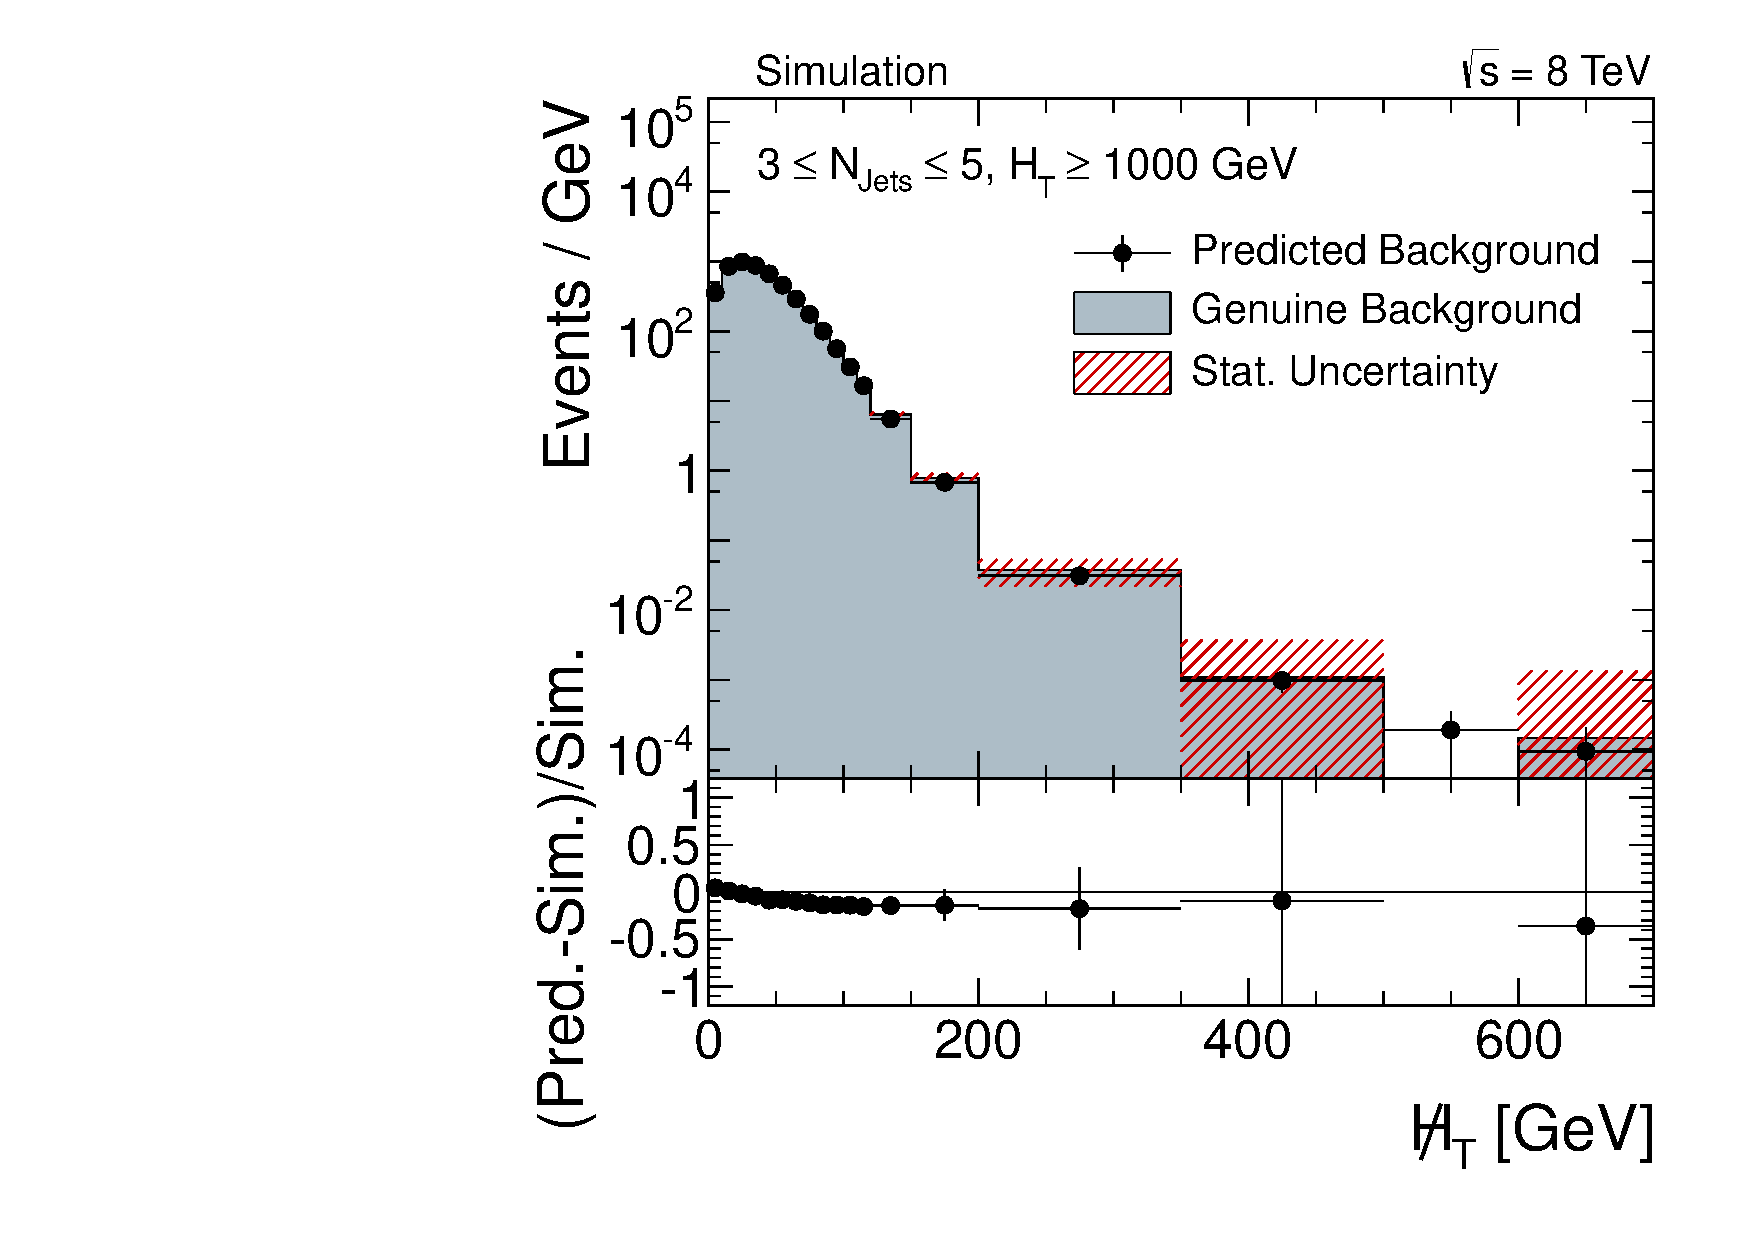
\includegraphics[width=0.49\textwidth]{figures/MHT_JetBin2_HThigh_madgraph_DR53X_chs_TuneZ2star_pt10_withoutPUReweighting_UseRebCorrection_v1.pdf}\\
                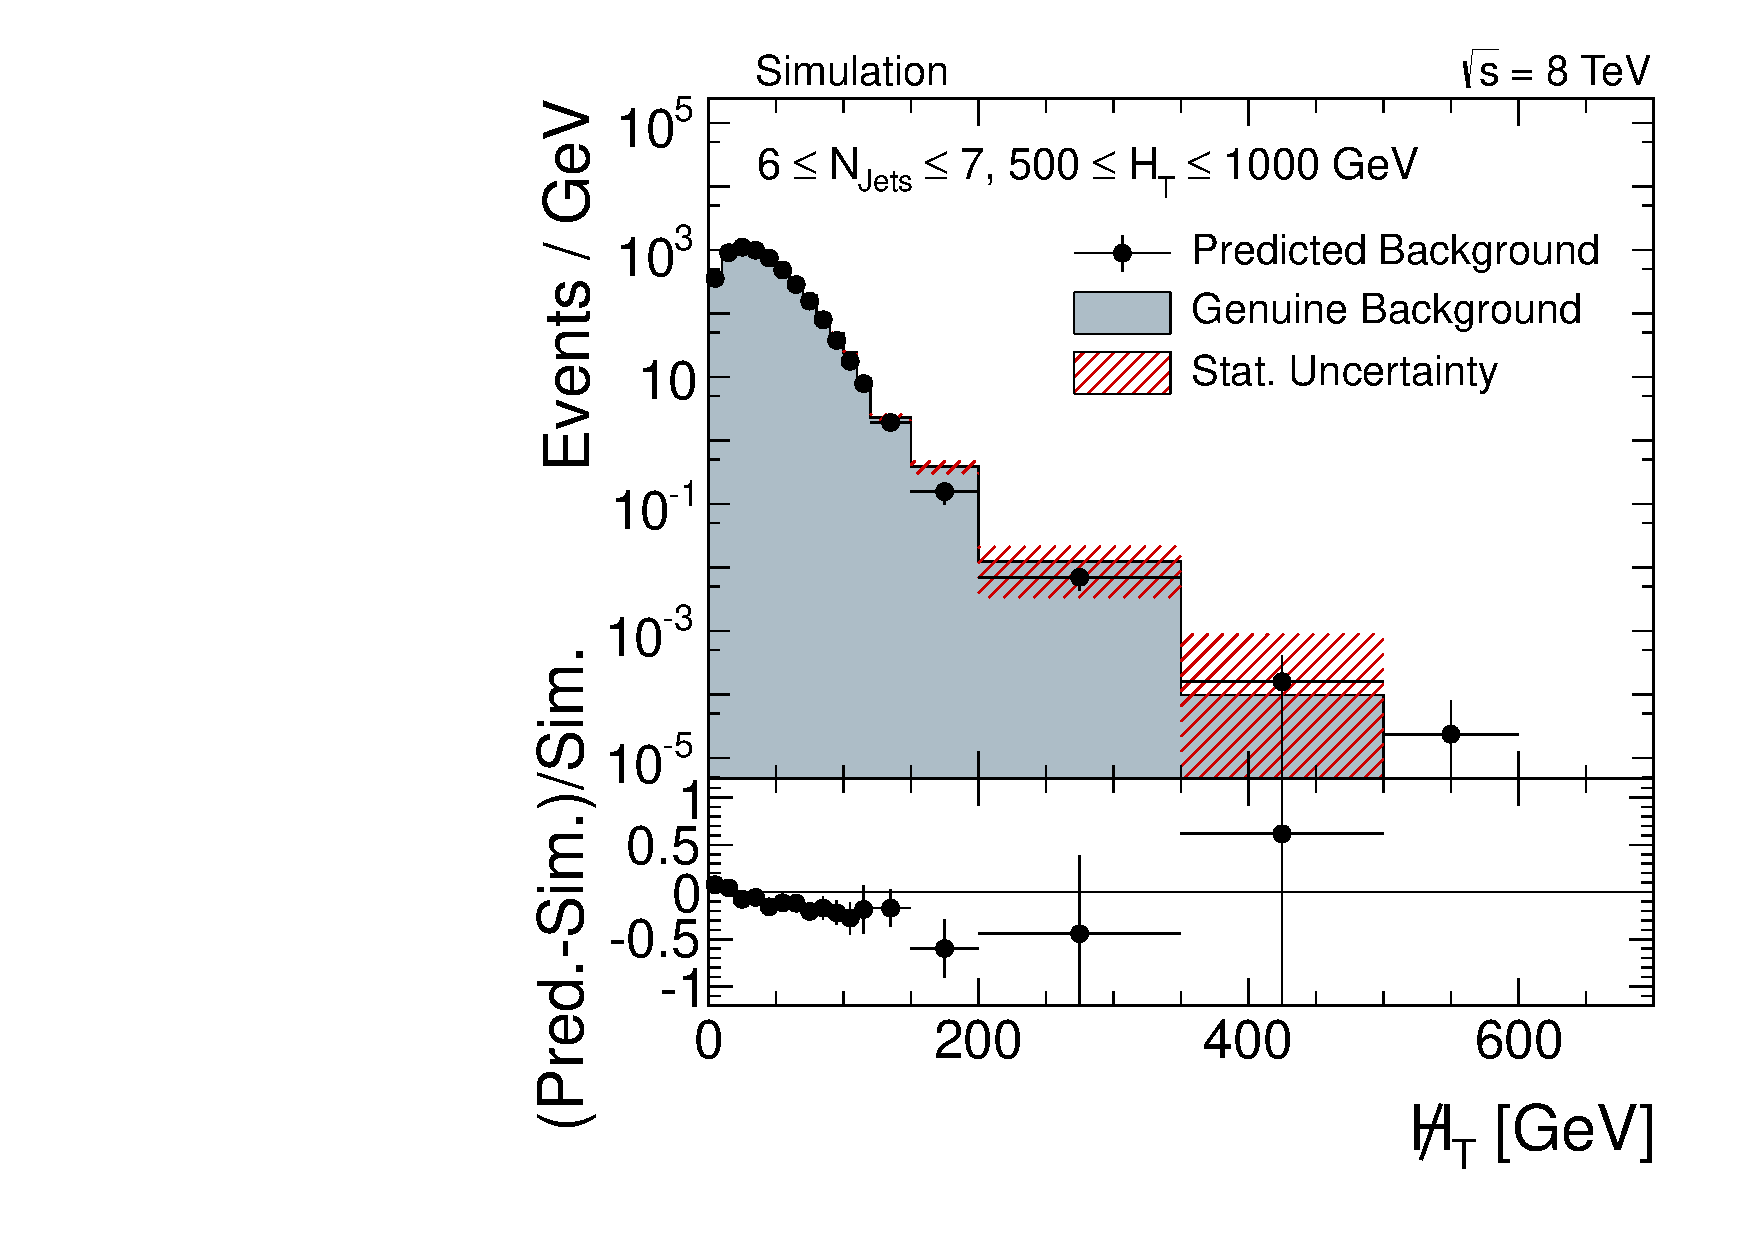
\includegraphics[width=0.49\textwidth]{figures/MHT_JetBin3_HTlow_madgraph_DR53X_chs_TuneZ2star_pt10_withoutPUReweighting_UseRebCorrection_v1.pdf} &
                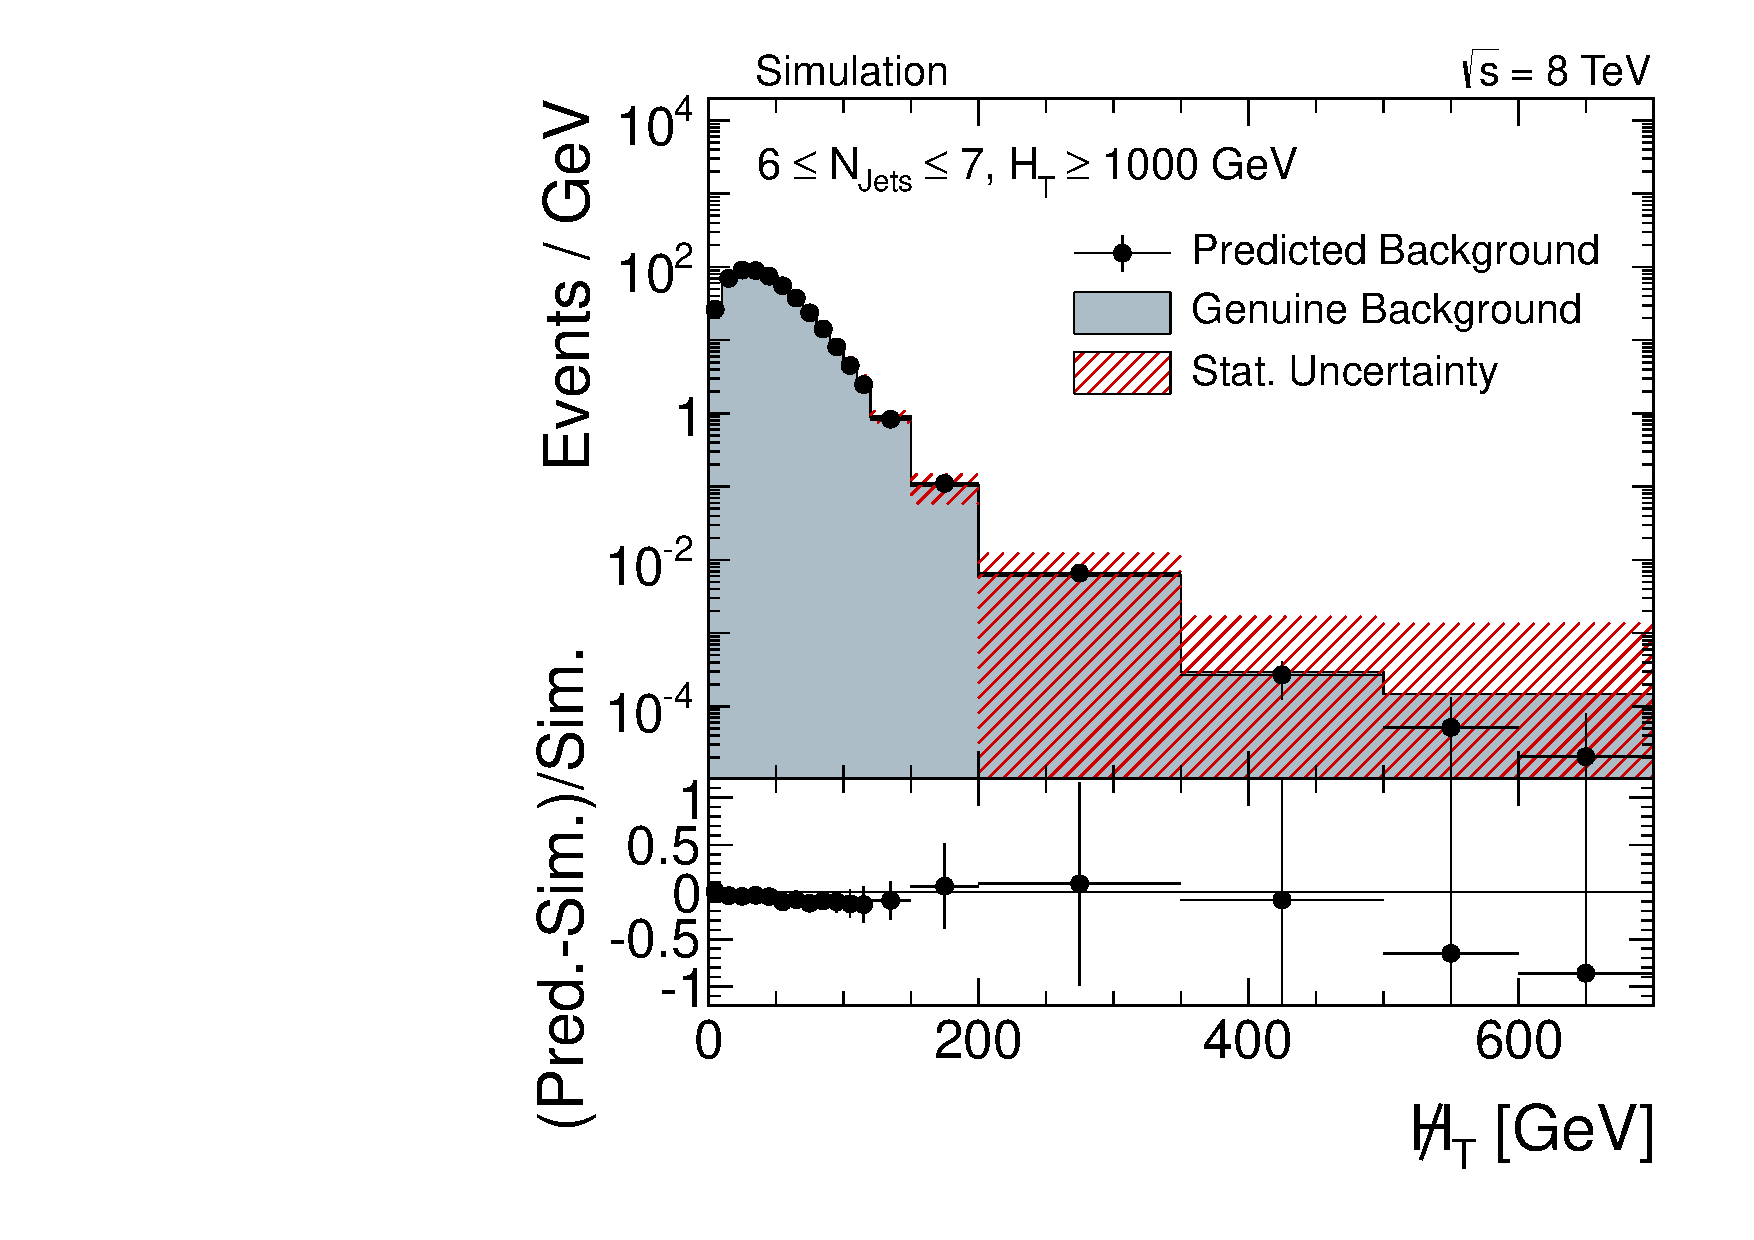
\includegraphics[width=0.49\textwidth]{figures/MHT_JetBin3_HThigh_madgraph_DR53X_chs_TuneZ2star_pt10_withoutPUReweighting_UseRebCorrection_v1.pdf}\\
                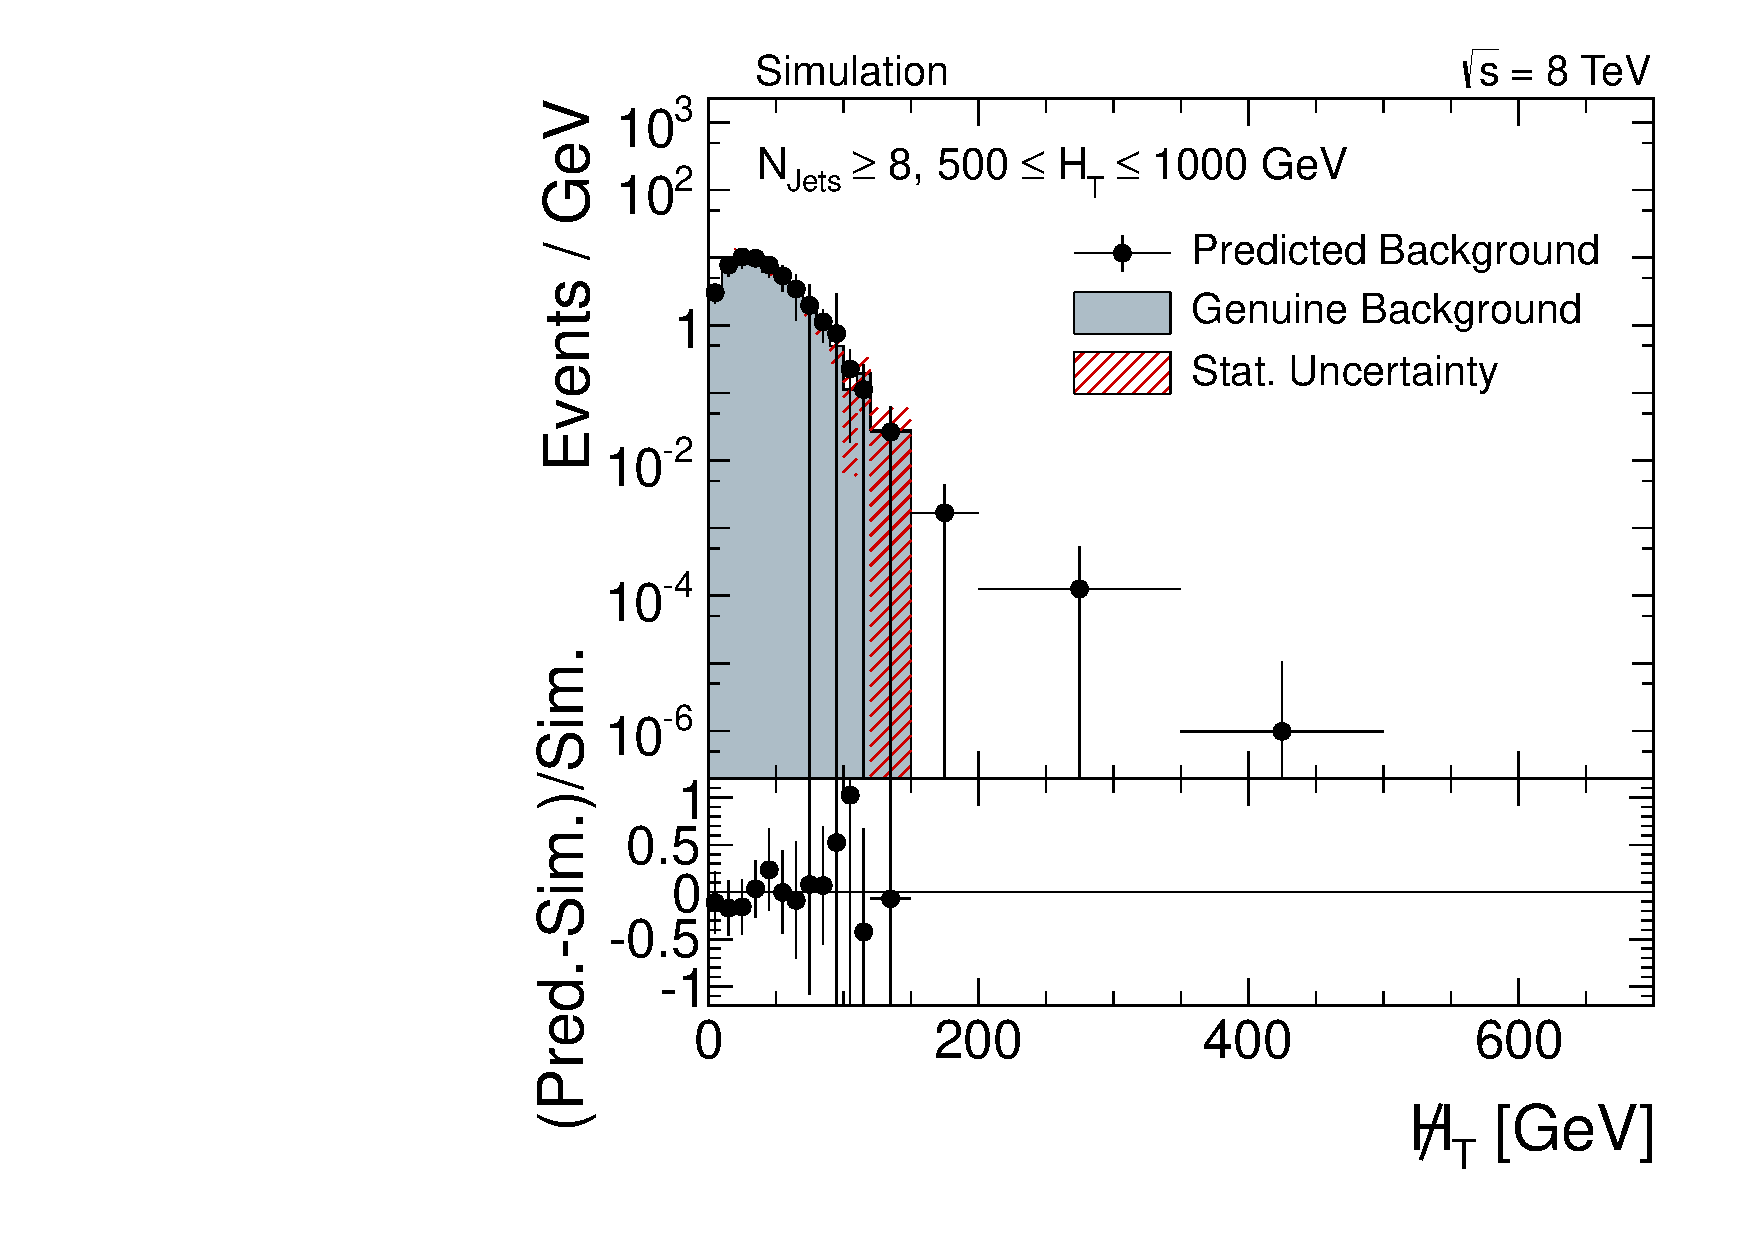
\includegraphics[width=0.49\textwidth]{figures/MHT_JetBin4_HTlow_madgraph_DR53X_chs_TuneZ2star_pt10_withoutPUReweighting_UseRebCorrection_v1.pdf} &
                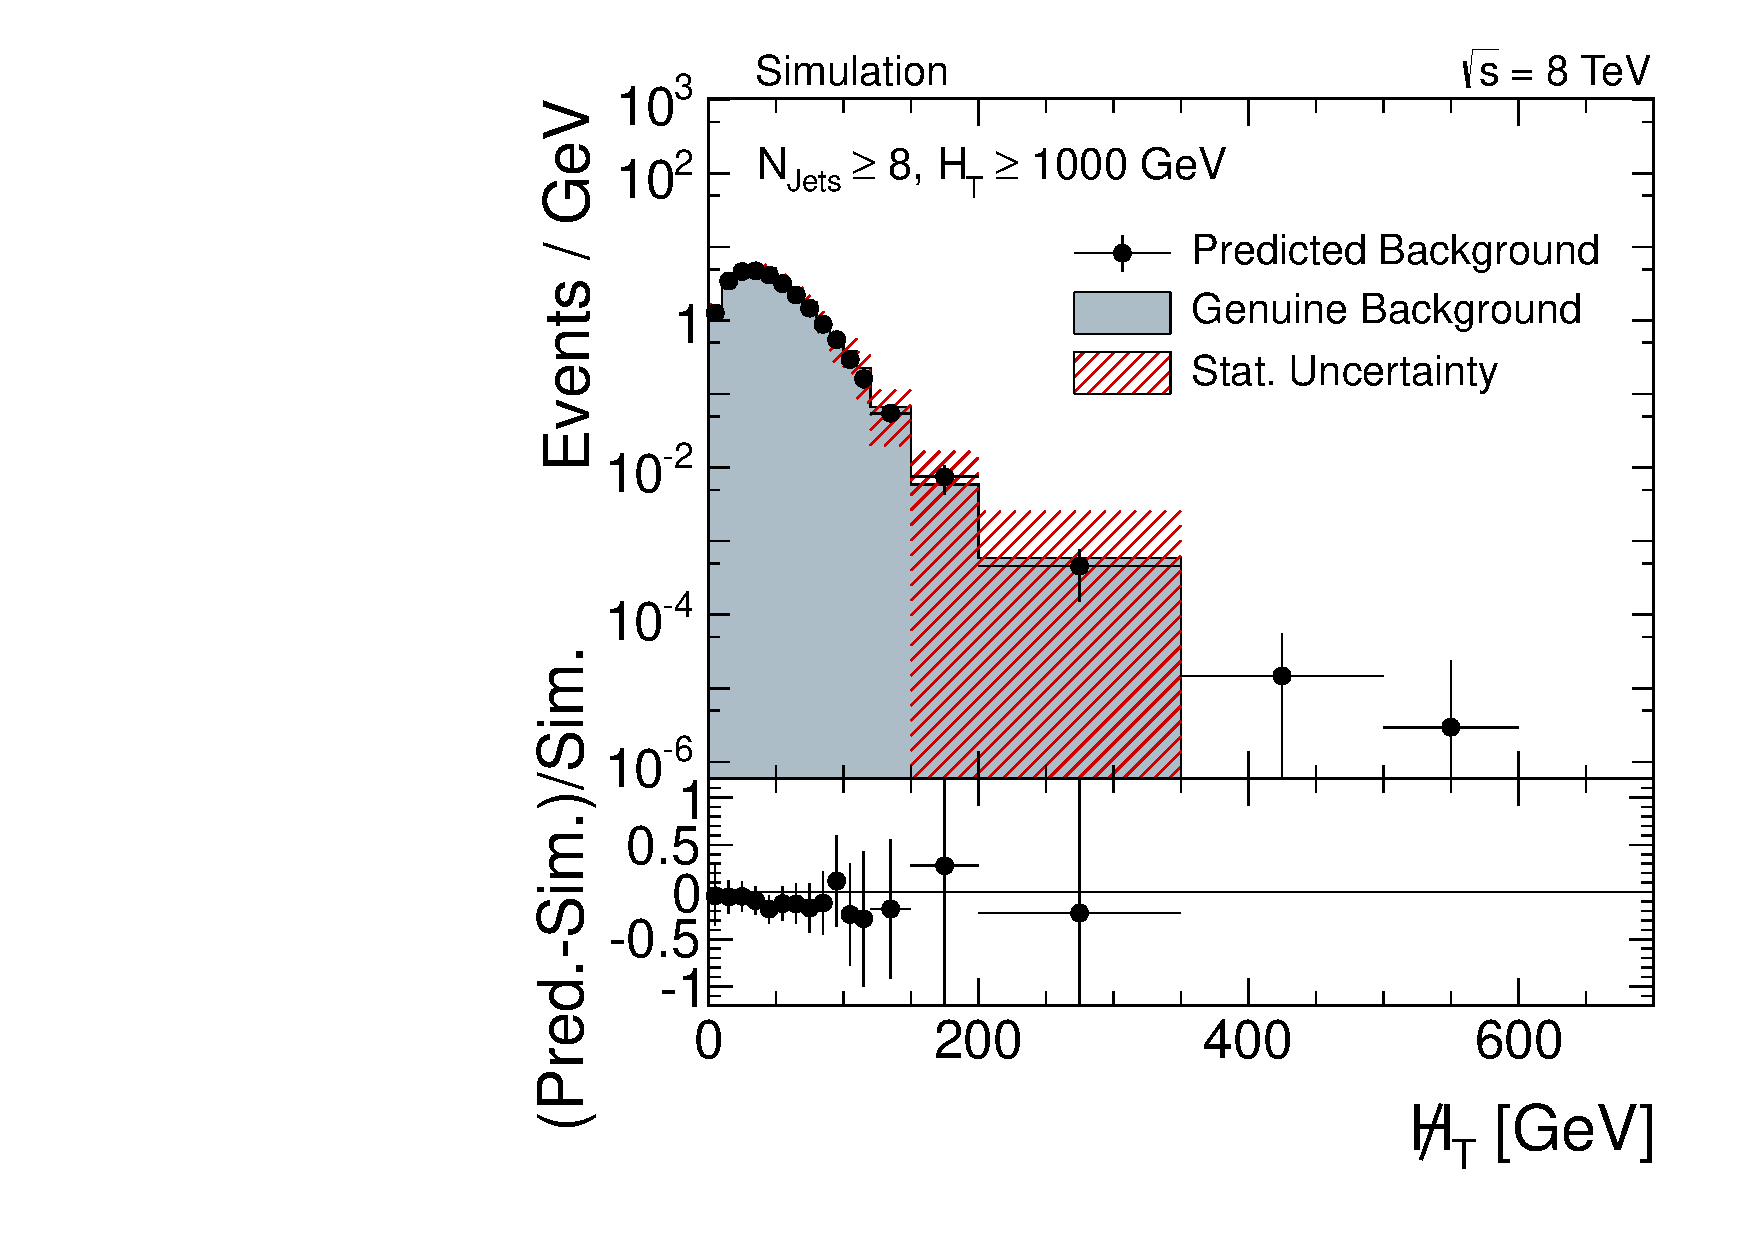
\includegraphics[width=0.49\textwidth]{figures/MHT_JetBin4_HThigh_madgraph_DR53X_chs_TuneZ2star_pt10_withoutPUReweighting_UseRebCorrection_v1.pdf}\\

  \end{tabular}
  \caption{Prediction of QCD background on a QCD multijet sample generated with \madgraph compared to the expectation from full simulation. The closure test is shown for various jet multiplicity bins and low (left) or high (right) \HT selections.}
  \label{fig:qcd_rs_closure}
\end{figure}
\begin{table}[!t] 
  \centering
  \caption{Summary of non-closure uncertainties with their statistical uncertainties derived for the signal region (\textit{first column}) and two control regions with \MHT $= 100 - 200$~GeV (\textit{second column}) and inverted $\Delta \phi$ criterium (\textit{third column}). The fourth column is used as additional cross check region, as described in the text. The numbers marked in bold letters are considered as the final non-closure uncertainties of the method.} 
  \label{tab:qcd_rs_closure_unc}
   \makebox[\linewidth]{
    \begin{tabular}{cc|cccc}
      \multicolumn{6}{c}{} \\
      \hline
      & & Signal region & Control region 1 & Control region 2 & Cross check region\\
      \hline
      $N_{\text{jets}}$ & \HT (GeV) & \MHT $>~200$ GeV &  \MHT $= 100 - 200$~GeV  &  \MHT $>~200$ GeV & \MHT $= 100 - 200$~GeV\\
      & & $\Delta \phi$ cut & $\Delta \phi$ cut & $\Delta \phi$ cut inverted & $\Delta \phi$ cut inverted\\
      \hline
      3 -- 5  & 500 -- 1000 & (\textbf{60.4} $\pm$~9.8)\% & (22.6 $\pm$~1.6)\% & (20.1 $\pm$~6.0)\% & (2.8 $\pm$~1.3)\%\\
      6 -- 7  & 500 -- 1000 & (43.1 $\pm$~46.5)\% & (\textbf{25.4} $\pm$~11.1)\% & (59.3 $\pm$~96.0)\% & (4.6 $\pm$~20.0)\%\\
      $\ge$ 8 & 500 -- 1000 & -- & (8.9 $\pm$~90.1)\% & (\textbf{86.0} $\pm$~38.2)\% & (12.2 $\pm$~66.4)\%\\
      \hline
      3 -- 5  & $\ge$ 1000 & (17.1 $\pm$~35.0)\% & (14.4 $\pm$~3.1)\% & (\textbf{14.5} $\pm$~8.9)\% & (5.1 $\pm$~1.7)\%\\
      6 -- 7  & $\ge$ 1000 & (5.5 $\pm$~108.0)\% & (\textbf{10.9} $\pm$~8.8)\% & (14.5 $\pm$~42.9)\% & (3.0 $\pm$~7.0)\%\\
      $\ge$ 8 & $\ge$ 1000 & (19.4 $\pm$~276.0)\% & (21.8 $\pm$~28.6)\% & (40.4 $\pm$~293.5)\% & (21.1 $\pm$~\textbf{42.6})\%\\
      \hline
    \end{tabular}}
\end{table}
\\
The first choice for the determination of remaining biases is to calculate the difference between prediction and expectation for the signal region, defined by \MHT $>$~200 GeV and the application of the $\Delta \phi$ cut, and take the observed difference as systematic uncertainty or even correct the prediction for a statistically significant non-closure of the method. The calculated differences with their statistical uncertainties for the signal region are summarized in Tab.~\ref{tab:qcd_rs_closure_unc} (first column). 
\\
The table exhibits that there is one bin ($3 \leq \NJets \leq 5$ and $500 \leq \HT \leq 1000$\gev) where the signal region shows a statistically significant non-closure. In Fig.~\ref{fig:qcd_rs_closure_comp}, this particular distribution is shown for the \madgraph QCD sample (left) and the \pythia sample (right). In the region for \MHT $=$ 200--350\gev, the \madgraph sample shows an underprediction of $\approx 60\%$, while the \pythia sample tends to a statistically not significant overprediction. Thus, it is difficult to judge, if this is really a systematic effect or just a statistical fluctuation. In order to treat this observed difference conservatively, the predicted result is not corrected for this potential deviation, but the total 60\% deviation in the \madgraph sample is considered as systematic uncertainty. As QCD is not the dominant background contribution in this search bin, this rather large uncertainty will hardly affect the final result of the analysis.
\begin{figure}[!t]
  \centering
  \begin{tabular}{cc}
                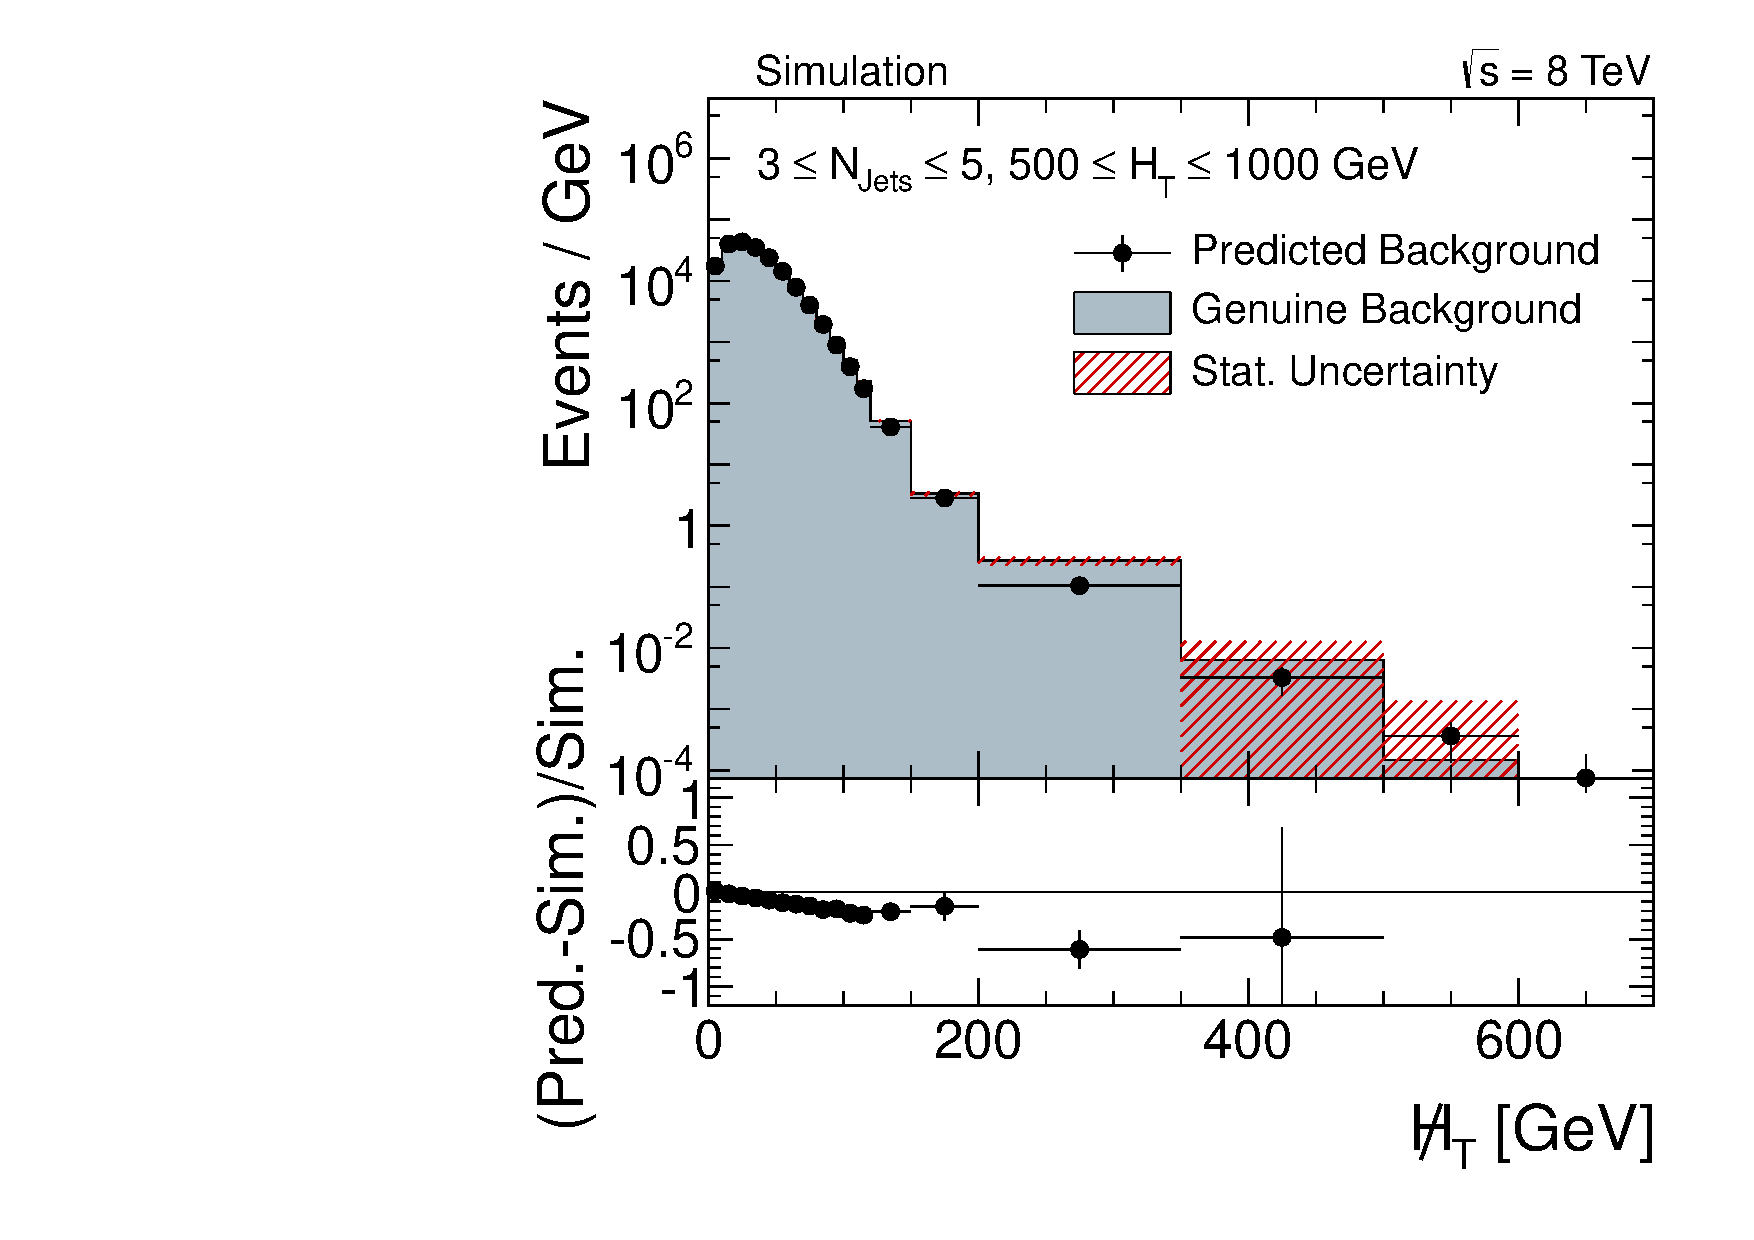
\includegraphics[width=0.49\textwidth]{figures/MHT_JetBin2_HTlow_madgraph_DR53X_chs_TuneZ2star_pt10_withoutPUReweighting_UseRebCorrection_v1.pdf} &
                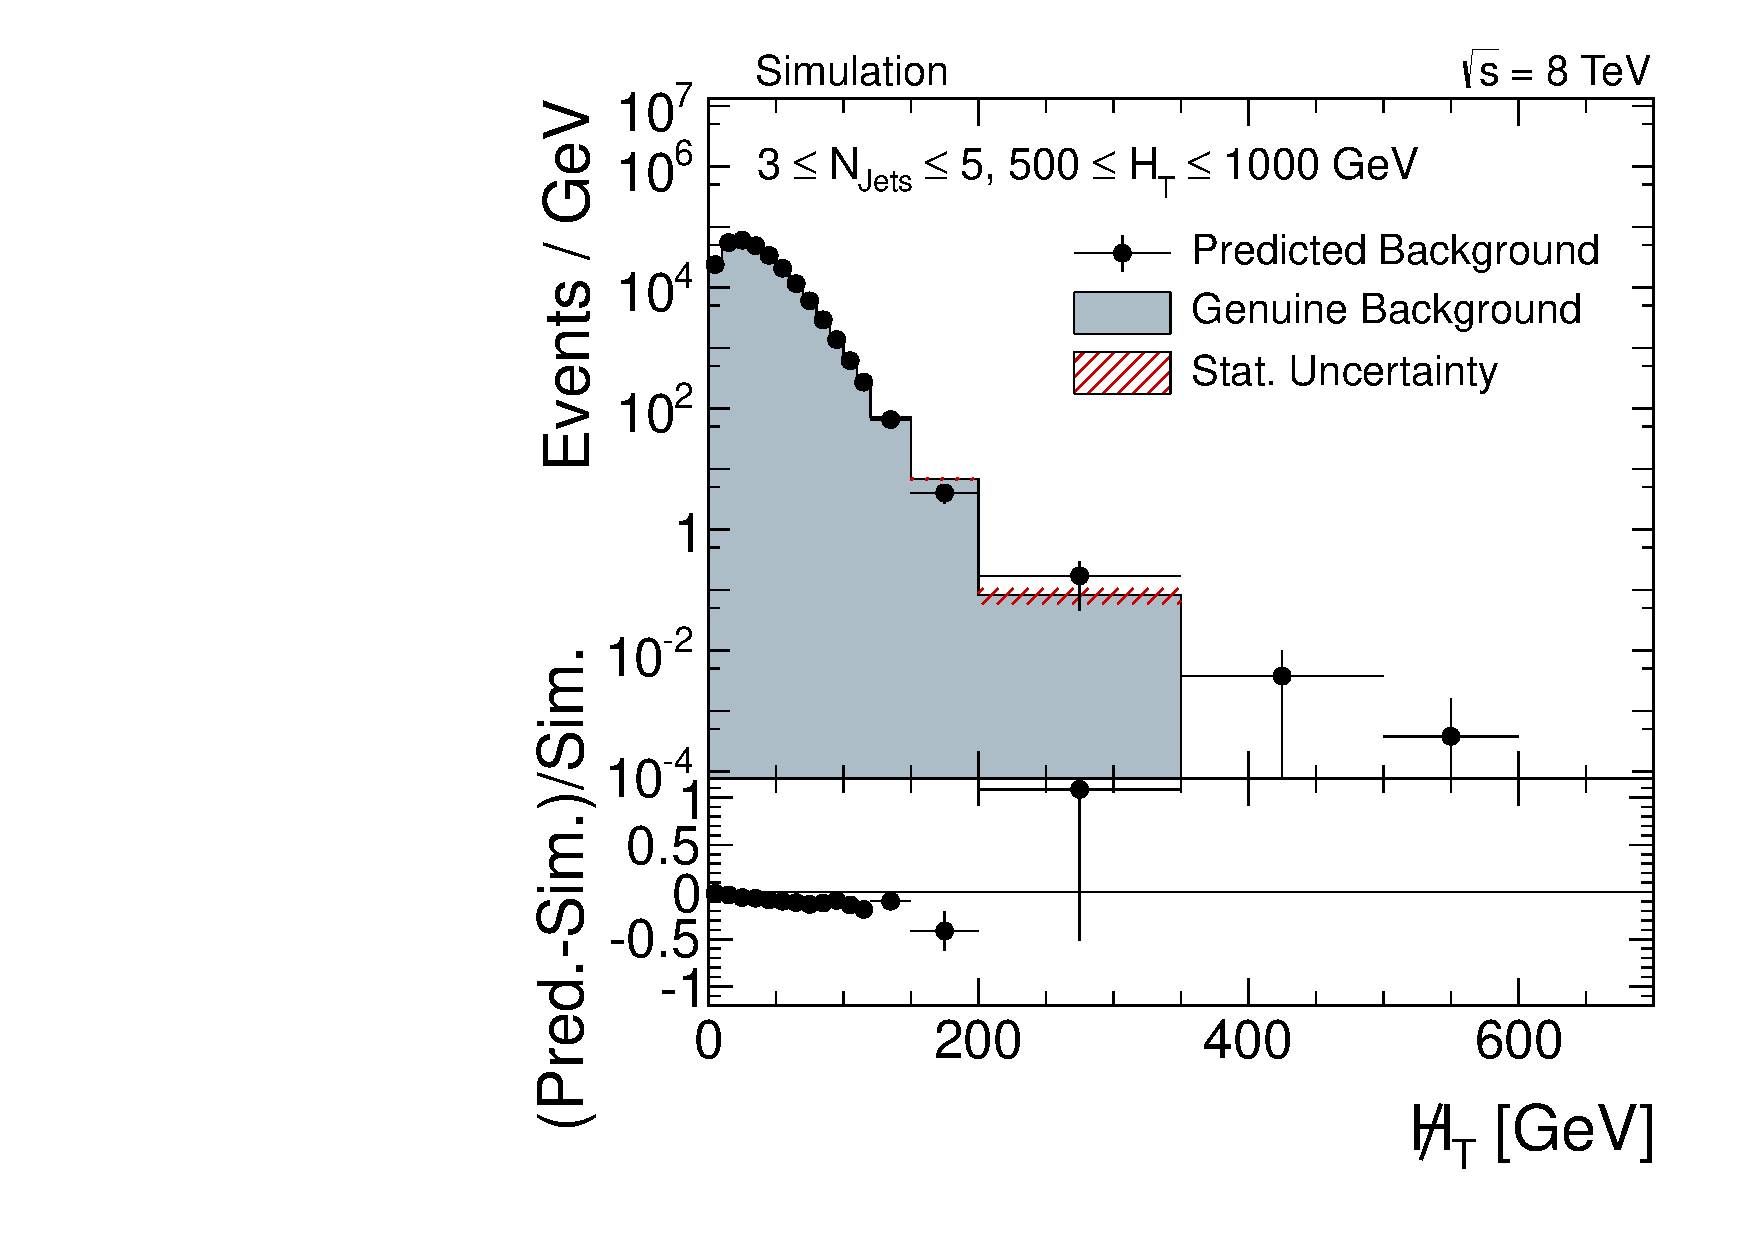
\includegraphics[width=0.49\textwidth]{figures/MHT_JetBin2_HTlow_pythia_DR53X_chs_TuneZ2star_pt10_withoutPUReweighting_UseRebCorrection_v1.pdf}\\
  \end{tabular}
  \caption{Prediction of QCD background on a simulated QCD multijet sample compared to the expectation from full simulation. The closure test is shown for 3-5 jets and $ 500 \leq \HT \leq 1000$~GeV on the \madgraph QCD sample (\textit{left}) and the \pythia QCD sample (\textit{right}).}
  \label{fig:qcd_rs_closure_comp}
\end{figure}
\\
Since the number of events in the signal region with $\MHT \ge 200$\gev is low for all bins except the one discussed above and thus the statistical uncertainties are large and do not lead to reasonable conclusions about the closure of the method, two sidebands of the signal region are studied. The prediction is compared to the full simulation either for control region 1 defined by $ 100 \leq \MHT \leq 200$\gev (second column in Tab.~\ref{tab:qcd_rs_closure_unc}) or for control region 2 defined by an inverted $\Delta \phi$ criterion (third column in Tab.~\ref{tab:qcd_rs_closure_unc}). The evaluation of the remaining bias aiming at a conservative treatment, proceeds as follows: 
\begin{itemize}
 \item If the differences in both control regions are statistically significant, the larger one is considered as systematic uncertainty. 
 \item If only one of the two numbers in the control regions is statistically significant, it has to be made sure that the assigned uncertainty by taking this number, \eg coming from control region 1, is not too small, as a remaining bias might come from the application of the $\Delta \phi$ cut. Thus, the value is compared to the value and its uncertainty in the corresponding cross check region bin (right column of Tab.~\ref{tab:qcd_rs_closure_unc}). If the value and its uncertainty in the cross check region are smaller than the chosen value from the control region, the number from the control region is considered as systematic error. Otherwise take largest number from cross check region (deviation or its uncertainty).
 \item If none of the numbers in the control regions is statistically significant, take the number with higher precision and proceed as above by comparing this value to the numbers in the cross check region. If the cross check region does not show larger values, take the number with highest precision, otherwise take largest number from cross check region.
\end{itemize}
The uncertainty which is finally considered by the procedure described above as the uncertainty quantifying the remaining bias of the R+S method, is printed in bold letters in Tab.~\ref{tab:qcd_rs_closure_unc}.

\subsection{Application to Data Events}
\label{subsec:validation_data_R+S}
\begin{figure}[!t]
  \centering
  \begin{tabular}{cc}
                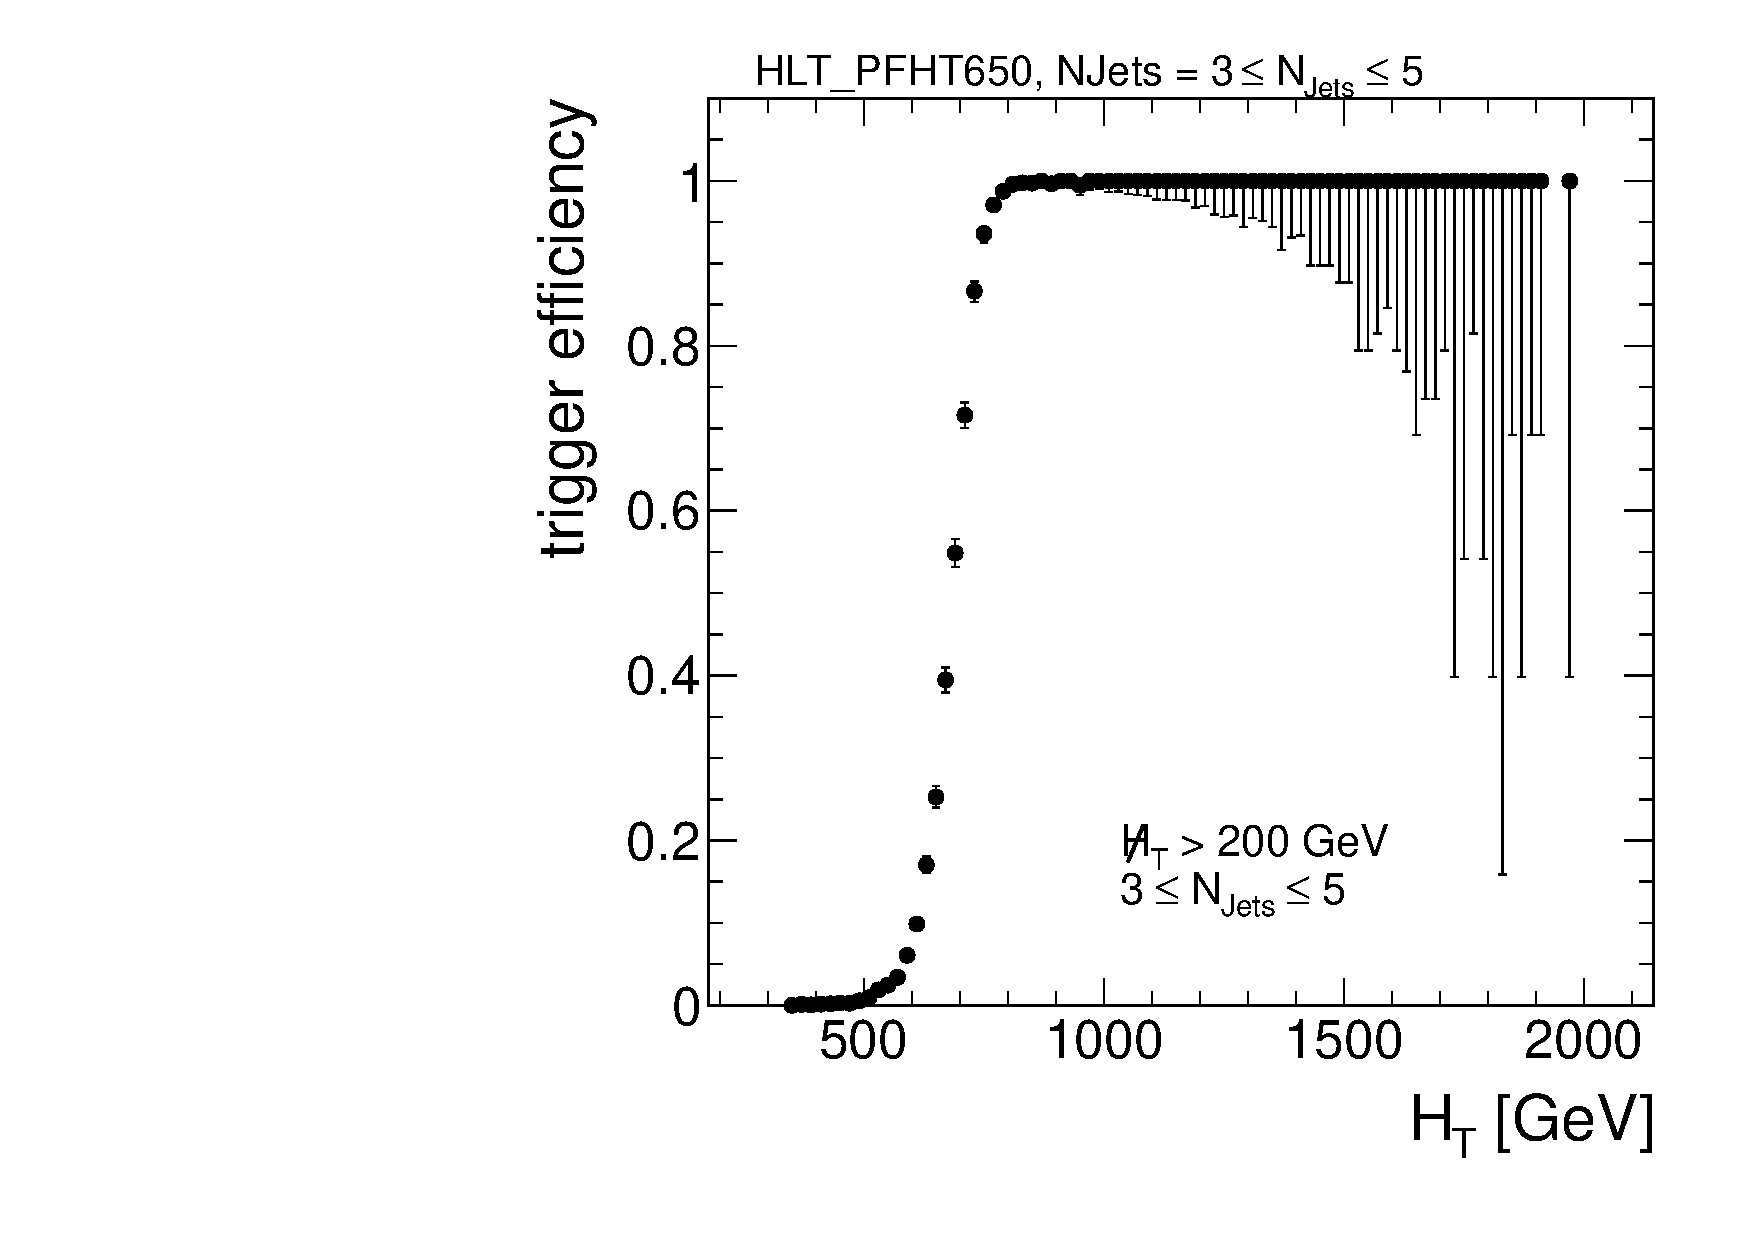
\includegraphics[width=0.49\textwidth]{figures/turn_on_HT_TagEle27WP80_ProbePFHT650_chs_NJets3-5.pdf} &
                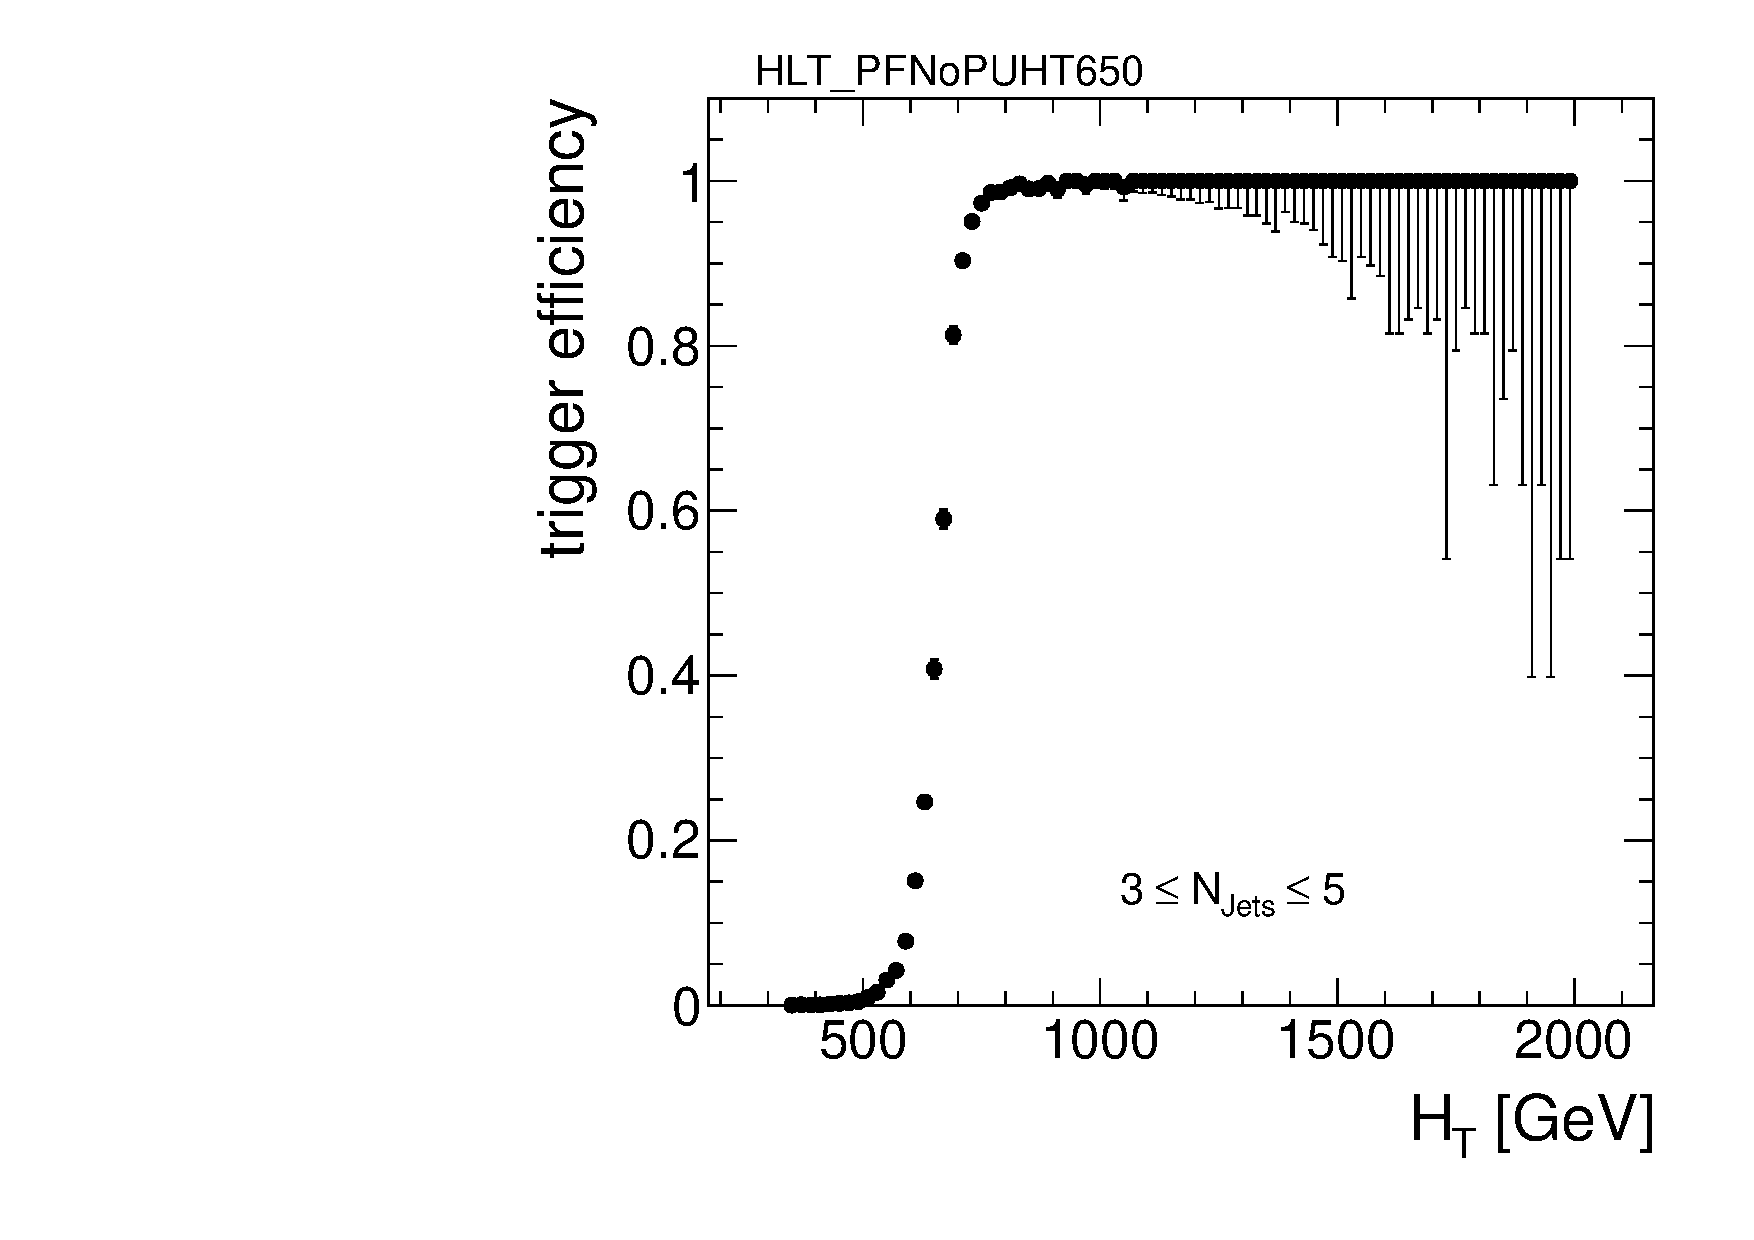
\includegraphics[width=0.49\textwidth]{figures/turn_on_HT_TagEle27WP80_ProbePFNoPUHT650_chs_NJets3-5.pdf} \\
  \end{tabular}
\caption{Measured trigger efficiency for paths HLT\_PFHT650 (\textit{left}) and HLT\_PFNoPUHT650 (\textit{right}) as a function of \HT, shown for $3 \leq$ \NJets $\leq 5$.} 
  \label{fig:trig_eff_650_3njets5}
\end{figure}
After the successful validation of the R+S method in simulated events and a quantification of a possible remaining bias, the procedure can finally be applied to data in order to estimate the QCD background contributions. \\
The QCD background prediction is performed on a QCD multijet data control sample. This is collected by two triggers based on \HT calculated from PF jets. The nominal \HT thresholds of the two triggers are 350\gev and 650\gev, respectively. The trigger efficiency as a function of \HT for a nominal threshold of 350\gev has been evaluated already for the signal trigger in Sec.~\ref{subsec:RA2_samples_trigger} and was observed to be fully efficient for the baseline \HT cut. The trigger efficiencies for the respective trigger with $\HT = 650$\gev are shown in Fig.~\ref{fig:trig_eff_650_3njets5} for a jet multiplicity of 3--5 and for jet multiplicities $6 \leq \NJets \leq 7$ and $8 \leq \NJets $ in App.~\ref{fig:trig_eff_650_6njets7} and App.~\ref{fig:trig_eff_650_njets8}, respectively. For these jet multiplicity selections, these two trigger paths are fully efficient for a \HT selection of 800\gev. \\
Since two different triggers are used, it has to made sure that each event of the multijet control sample is unambigously assigned to only one trigger to avoid double-counting of certain events and gain a smooth \HT spectrum to not bias the background prediction. Taking into account that the trigger with the lower \HT threshold has been prescaled during operation, this is done as follows: For each event, the trigger which fired and has the lowest prescale factor is determined. Then the event is weighted according to this prescale factor. Since only one prescaled and one unprescaled trigger is considered, this assignment is unambigious and leads to a smooth \HT spectrum which starts at the lowest trigger threshold. The prescale weighted seed \HT distribution is illustrated in Fig.~\ref{fig:qcd_rs_seedht}.
\begin{figure}[!t]
  \centering
  \begin{tabular}{c}
                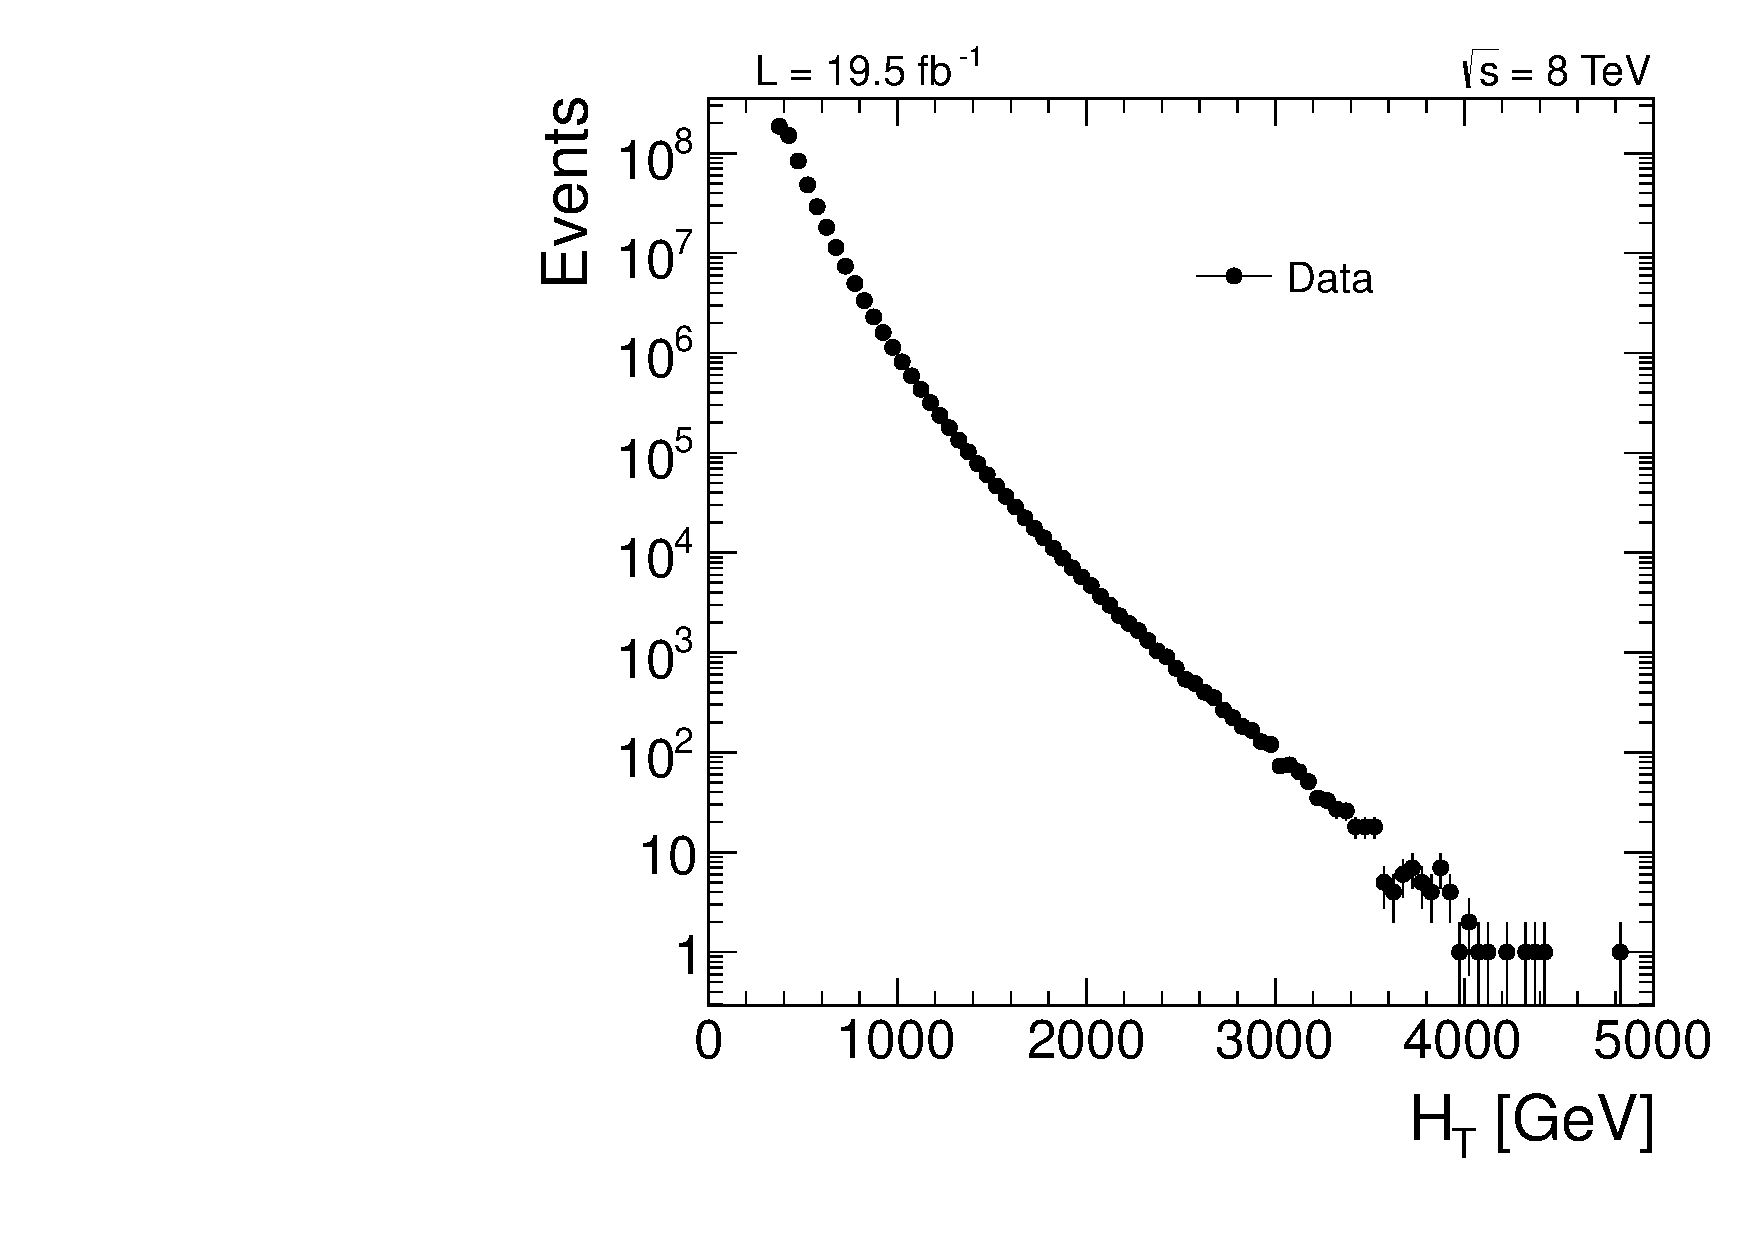
\includegraphics[width=0.49\textwidth]{figures/HT_data.pdf}
  \end{tabular}
  \caption{Seed \HT spectrum of full 2012 dataset used as input for the R+S method after correcting for trigger prescales.}
  \label{fig:qcd_rs_seedht}
\end{figure}
The usage of prescaled triggers is important in order to collect also events with \HT values smaller than 500\gev which enter the signal region through a fluctuation to large response values. Nevertheless, the events collected by the prescaled trigger come along with high event weights and spoil artifically the prediction when they enter the signal region as they lead to a substantially higher standard deviation. This problem is solved by smearing the events obtained from the prescaled trigger not only $N = 100$ times, but $N = \rm{prescale~factor} \times 100$ times and weighting them accordingly with one.\\
\\
The successful application of the R+S method to data can be validated. This is done by comparing the prediction with the R+S method from data to selected events in a QCD enriched data control sample. This control sample is defined by at least three jets, $\HT > 1000$\gev, an inverted $\Delta \phi$ criterion and $100 \leq \MHT \leq 200$\gev. The resulting comparison between predicted and selected data events in that region is shown in Fig.~\ref{fig:qcd_rs_dataclosure} and exhibits reasonable agreement. Furthermore, no perfect agreement is expected since contaminations from other backgrounds are still present. \\
Overall, the application of the R+S method to predict the QCD background contributions in data is expected to provide reliable results, since the validation tests in simulation as well as in data have a positive outcome. However, systematic uncertainties that have to be considered for the prediction of QCD background are discussed in the next section. 
\begin{figure}[!t]
  \centering
  \begin{tabular}{cc}
                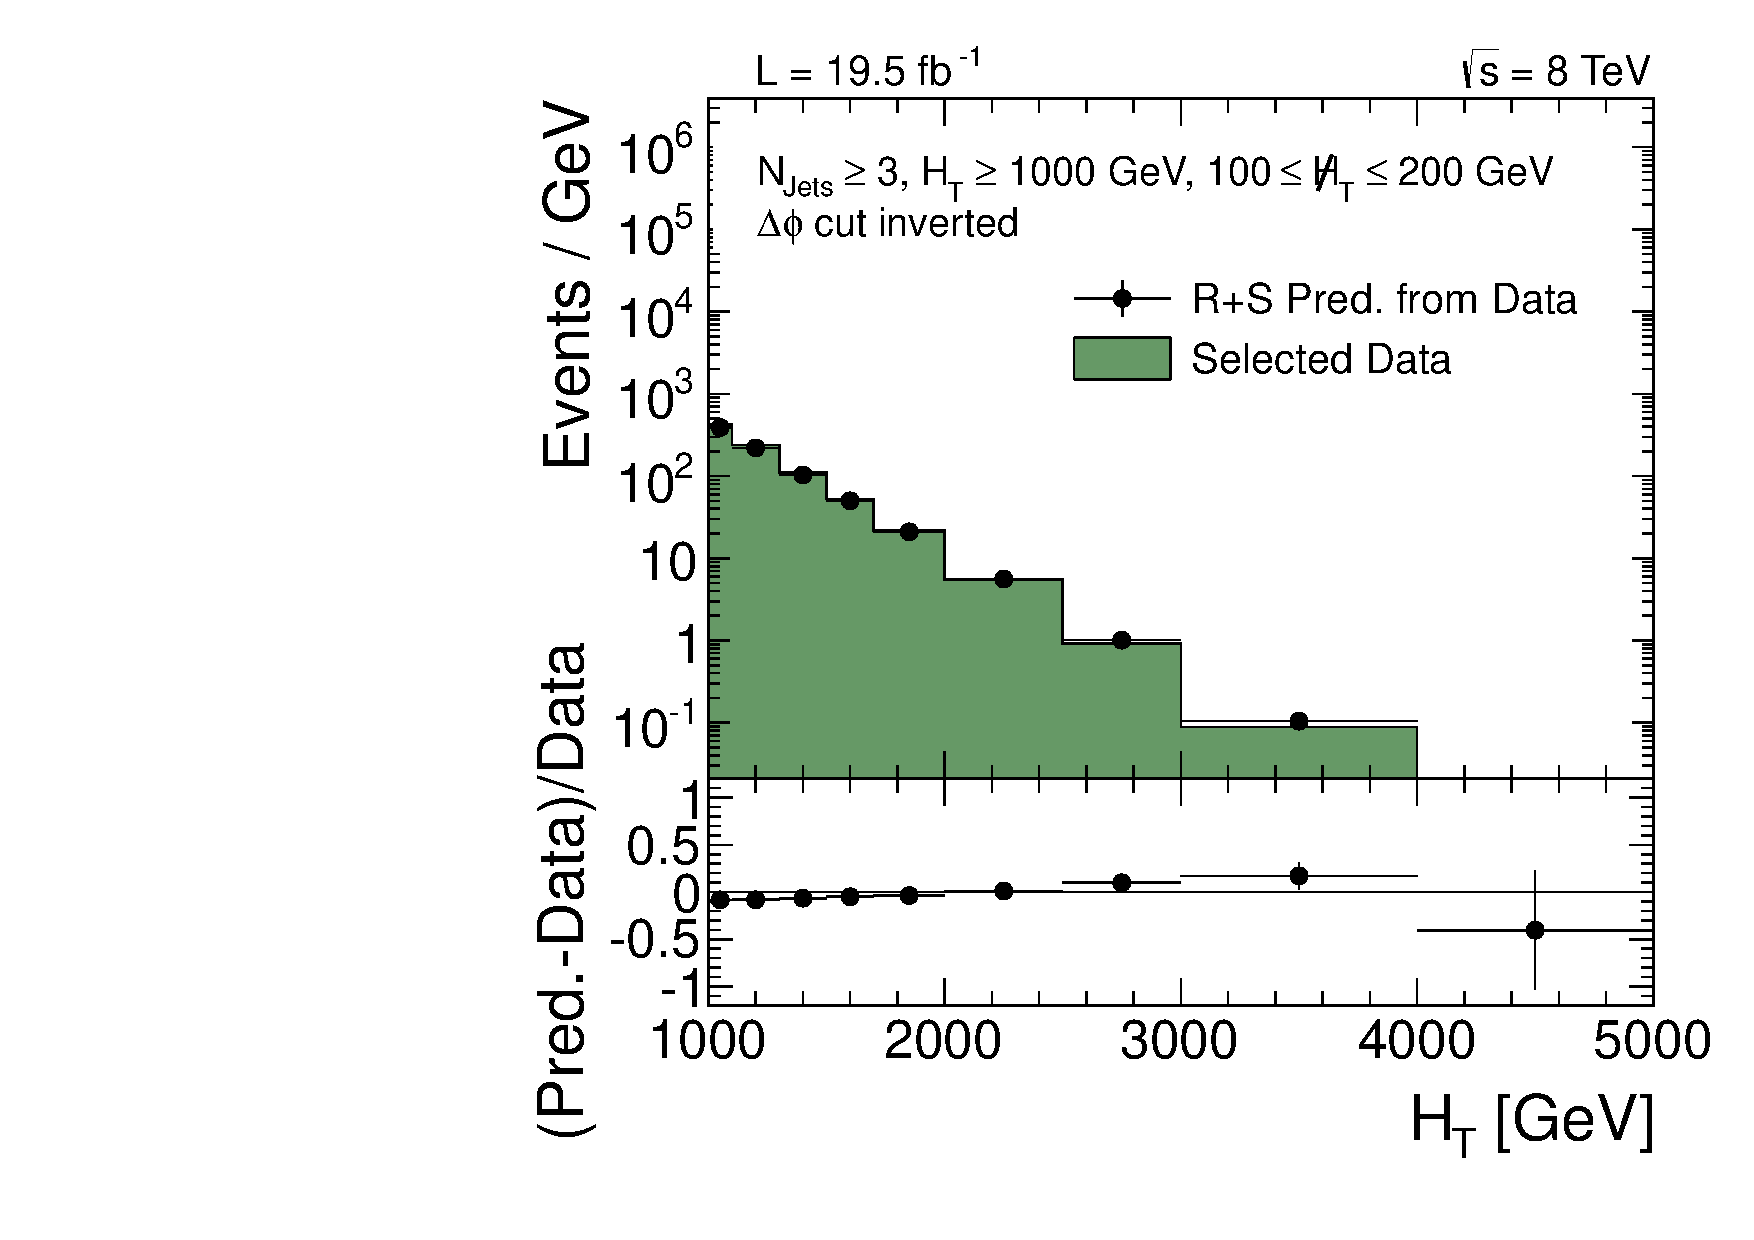
\includegraphics[width=0.49\textwidth]{figures/HT_presel_HThigh_data_DR53X_chs_HThigh_invertedDeltaPhi_v1.pdf} &
                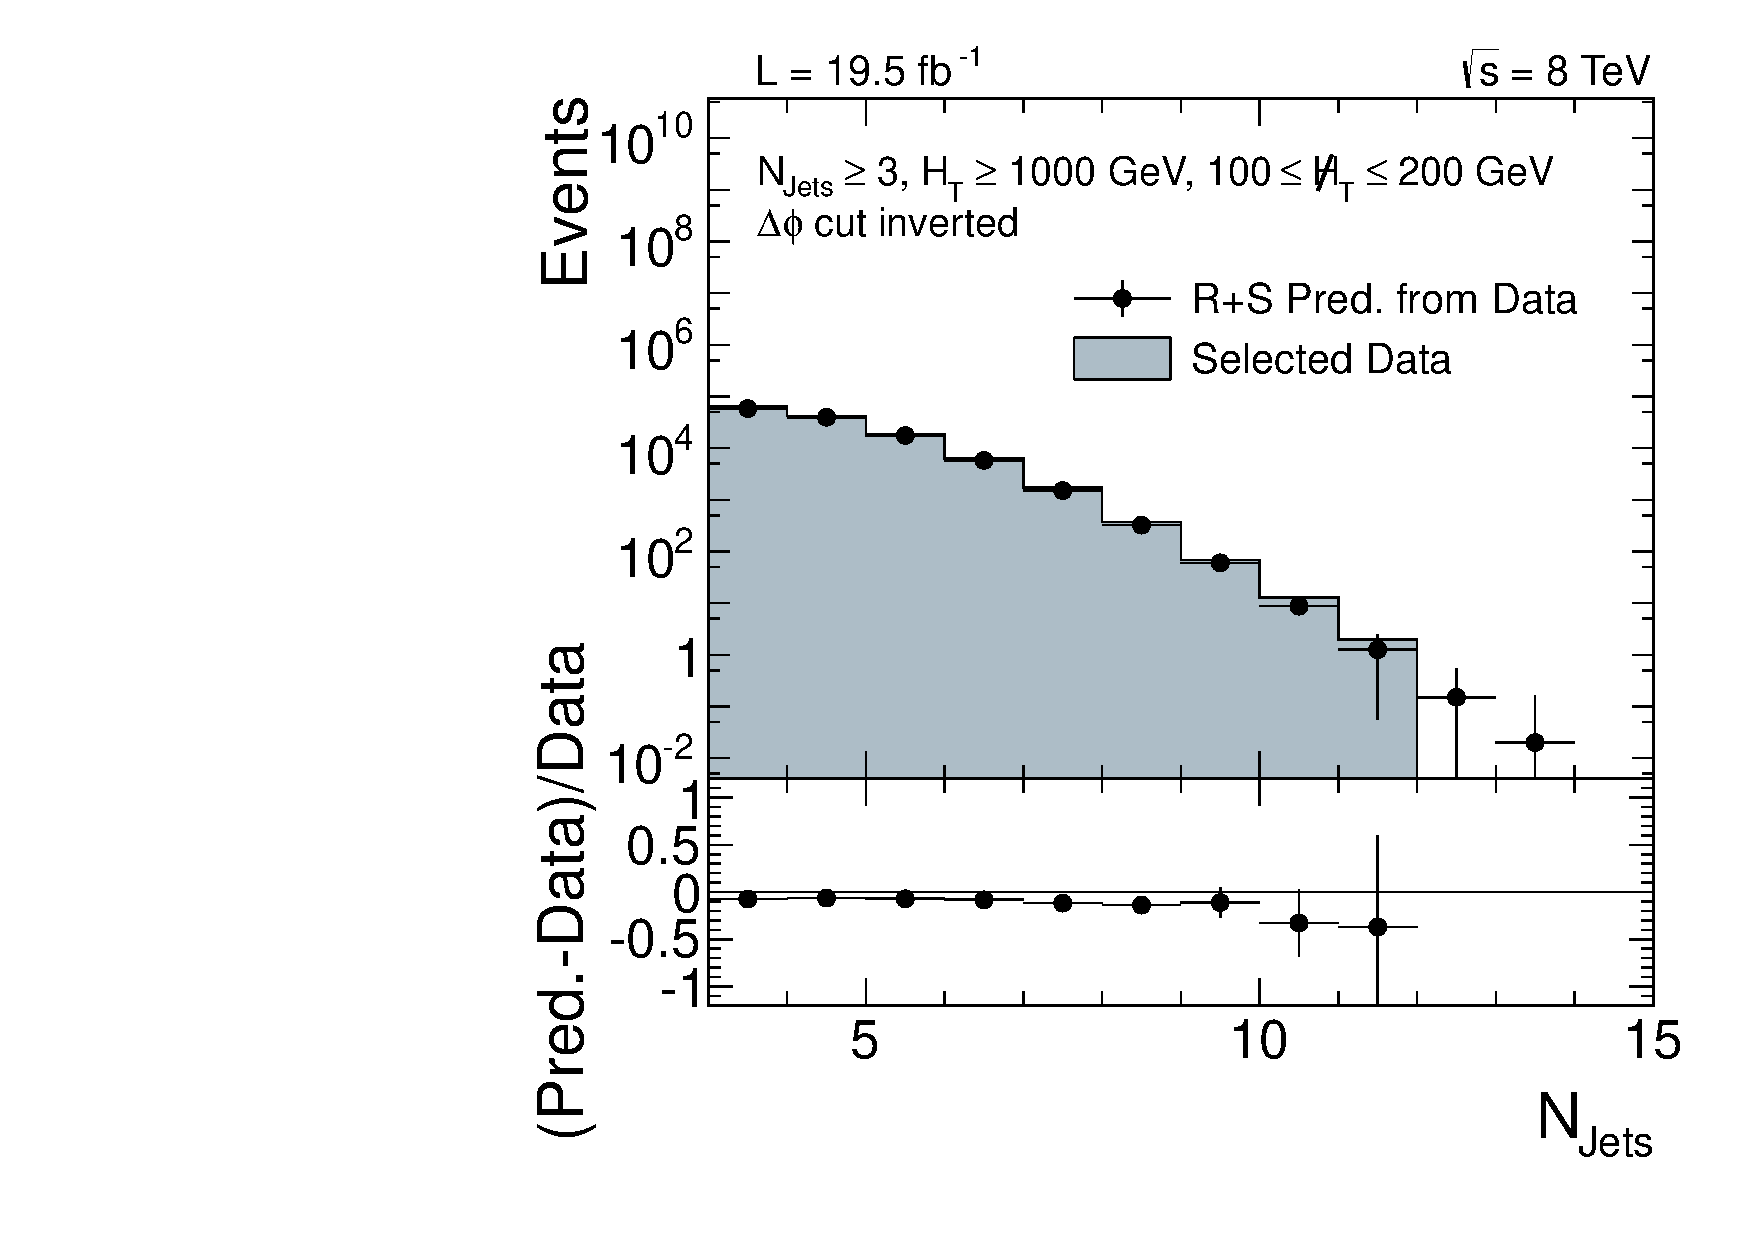
\includegraphics[width=0.49\textwidth]{figures/NJets_presel_HThigh_data_DR53X_chs_HThigh_invertedDeltaPhi_v1.pdf} \\
  \end{tabular}
  \caption{Prediction of QCD background on data compared to the expectation from data for a QCD enriched control region with \HT$>~1000~\rm{GeV}$, inverted $\Delta \phi$ cut, $\NJets \geq 3$ and $100 \leq \MHT \leq 200$\gev.}
  \label{fig:qcd_rs_dataclosure}
\end{figure}

\subsection{Systematic Uncertainties}
\label{subsec:RA2_syst_unc}
Different systematic uncertainties of the R+S method have been evaluated:
\begin{itemize}
\item \textbf{Core of response functions:} The uncertainties on the factors of the Gaussian core resolution accounting for the differences in data and Monte Carlo denoted in Tab.~\ref{tab:jer_RPlusS_core} are propagated to the prediction. This is done by shifting the scaling factors by $\pm 1\sigma$ up and down. 
\item \textbf{Tail of response functions:} The uncertainties on the scaling factors of the non-Gaussian tails listed in Tab.~\ref{tab:jer_RPlusS_tails} are also propagated to the prediction by varying them within $\pm 1\sigma$ up and down. 
\item \textbf{Non-closure:} The systematic uncertainty due to a potential non-closure and remaining biases of the R+S method is evaluated as described in Sec.~\ref{subsec:validation_mc}. This uncertainty also covers uncertainties on the rebalance correction factor and the jet-\pt cut value chosen for the jets considered in the rebalancing, such that no additional uncertainties are considered for those. The bias uncertainty is evaluated for each jet multiplicity bin separated into a low $ 500 \leq \HT \leq 1000$\gev and a high $\HT > 1000$\gev region.
\item \textbf{Pileup:} In general, the R+S method is taking care of influences from pileup by applying L1 corrections to the jet momenta, making use of charged-hadron subtraction and neglecting soft jets in the rebalancing procedure. Furthermore, pileup which is an issue especially for soft jets does in general not contribute significantly to the high \MHT search bins, as these are mainly populated due to heavily mismeasured hard jets. Thus, a valid approach to evaluate possible residual pileup effects is to use a low \MHT control region with \MHT $> 100 \rm{~GeV}$. This approach also ensures that statistical limitations are reduced.\\
The general approach is to study the difference in the behaviour of the prediction in data and simulation (taken from \madgraph) for different pileup conditions. Hence, the sample is divided into three different bins of primary vertices $N_\mathrm{Vtx} = [0$--$10]$, $N_\mathrm{Vtx} = [11$--$20]$ and $N_\mathrm{Vtx} > 20$. The QCD prediction for each vertex bin is calculated for \HT $>500$\gev and $\Delta \phi$ cut applied, and normalized to the number of seed events contributing to that particular vertex bin. It is assumed that pileup effects are negligible in the lowest primary vertex bin. Thus, the predictions corrected for the number of seed events in data and simulation are normalized to each other, such that they have the same yield in the first primary vertex bin. This distribution is illustrated for jet multiplicity 3--5 jets in Fig.~\ref{fig:qcd_rs_pileup}. 
\end{itemize}
\begin{figure}[!h]
  \centering
  \begin{tabular}{cc}
                \includegraphics[width=0.49\textwidth]{figures/PUUncertainty_NJet3_5.pdf}% &
  %              \includegraphics[width=0.49\textwidth]{figures/PUUncertainty_NJet6_7.pdf} \\
  %              \multicolumn{2}{c}{\includegraphics[width=0.49\textwidth]{figures/PUUncertainty_NJet8.pdf}}
  \end{tabular}
  \caption{Prediction of QCD background in data and Monte Carlo as a function of primary vertices ($N_\mathrm{Vtx}$) normalized to the number of contributing seed events used for the determination of the pile-up uncertainty as described in Sec.~\ref{subsec:RA2_syst_unc}.}
  \label{fig:qcd_rs_pileup}
\end{figure}
Then, the absolute difference between data and Monte Carlo prediction is calculated for the second and the third vertex bin, multiplied each with the seed events in data for that vertex bin and summed up. %The input distributions for this calculation are illustrated in Fig.~\ref{fig:qcd_rs_pileup}. 
The calculated ratio of this pileup dependent fraction of the prediction to the nominal QCD prediction is considered as pileup uncertainty. It is evaluated for each jet multiplicity interval separately. 

\subsection{QCD Background Prediction}
\label{subsec:RA2_qcd_pred}
The final prediction for QCD background contributions derived with the R+S method from a multijet control sample in data is summarized in Tab.~\ref{tab:QCDPred} for jet multiplicity bins 3--5, 6--7 and $\ge 8$. The quoted total systematic uncertainty is obtained by adding the single contributions in quadrature. \\
Some search bins show very large statistical uncertainties of $\geq 100 \%$ which then also affects the evaluation of systematic effects, \eg the core and tail scaling uncertainties. However, since this happens only in bins where QCD background is almost negligible, it does not impact the final result of the analysis significantly. For the affected systematic variations, the largest observed variation is considered as systematic uncertainty as a conservative estimate. Search bins that are affected by that are mainly the high \MHT and the highest jet multiplicity search bins. \\
However, search regions with non-negligible contributions from QCD background, like high \HT ($\ge 1000$\gev) and low \MHT bins, in general show quite moderate total uncertainties around only 50\% which is a remarkable result for a prediction of a background that is that difficult to model, as discussed in the beginning of this section. The main contributions to the systematic uncertainty arise from the propagated uncertainties of the core and tail scaling factors. The resulting variations in the prediction from the variation of the core scaling factors are typically between 10--30 $\%$ in the search bins with non-negligible QCD contributions while it is between 20--35 $\%$ from the tail scaling factors. This emphasizes the importance to precisely measure the resolution data-to-simulation scale factors, as described in Chap.~\ref{chap:Resolution} for the scaling factors of the response core. 
\begin{table}[!hp]
  \centering
  \caption{Predicted event yields for the QCD background in the search regions defined by \HT, \MHT and \NJets shown together with statistical and systematic uncertainties. The uncertainties of the different systematic uncertainty sources are added in quadrature to obtain the total systematic uncertainties.}
  \label{tab:QCDPred}
  \makebox[\linewidth]{
    % \begin{tabular*}{\textwidth}{lll@{\extracolsep{\fill}}|r|r|r|r|r|r}
   % \begin{tabular}{lll|r|l|c|c|c|c|c}
    \begin{tabular}{lll|rc|cccc|c}
      \multicolumn{10}{c}{} \\
    

  %    \NJets{} & \HT{} [GeV] &\MHT{} [GeV]
      \NJets{} & \HT{} [GeV]& \MHT{} [GeV] & Pred. & stat. unc. & Core [\%] & Tail [\%] & Bias [\%] & PU [\%] & syst. unc. \\
      \midrule
      3-5     & 500-800  & 200-300 & 307.4 & $\pm$  18.5  & $^{+13.0}_{-12.2}$ & $^{36.0}_{-34.4} $ & $\pm$ 60.4 & $\pm$ 2.9 & $^{+220}_{-217}$  \\
      3-5     & 500-800  & 300-450 & 34.5  & $\pm$  5.8   & $^{+7.3}_{-10.5}$ & $^{22.9}_{-31.6} $  & $\pm$ 60.4 & $\pm$ 2.9 & $^{+22.4}_{-23.8}$ \\
      3-5     & 500-800  & 450-600 & 1.3   & $\pm$  1.2   & $^{+24.2}_{-16.7}$ & $^{+37.9}_{-26.5}$ &  $\pm$ 60.4 & $\pm$ 2.9 & $^{+1.0}_{-0.9}$  \\
      3-5     & 500-800  & $>600$  & 0.1   & $\pm$  0.3   & $^{+55.6}_{-55.6}$ & $^{+55.6}_{-55.6}$ & $\pm$  60.4 & $\pm$ 2.9 & $^{+0.09}_{-0.09}$\\ 
      \midrule
      3-5    & 800-1000  & 200-300 & 91.7  & $\pm$  10.2  & $^{+14.7}_{-13.8}$  & $^{+33.2}_{-33.5}$ & $\pm$  60.4 & $\pm$ 2.9 & $^{+64.7}_{-64.7}$\\
      3-5    & 800-1000  & 300-450 & 9.9   & $\pm$  3.2   & $^{+5.2}_{-5.1}$ & $^{+29.8}_{-27.1}$  & $\pm$  60.4  & $\pm$ 2.9 & $^{+6.7}_{-6.6}$ \\
      3-5    & 800-1000  & 450-600 & 0.8   & $\pm$  0.9  & $^{+65.5}_{-65.5}$ &  $^{+65.5}_{-65.5}$ & $\pm$  60.4 & $\pm$ 2.9 & $^{+0.9}_{-0.8}$  \\
      3-5    & 800-1000  & $>600$  & 0.1   & $\pm$  0.4  & $^{+75.0}_{-41.7}$ &  $^{+8.3}_{-41.7}$  & $\pm$  60.4 & $\pm$ 2.9 & $^{+0.1}_{-0.1}$  \\
      \midrule
      3-5   & 1000-1250  & 200-300 & 59.0  & $\pm$  7.2  & $^{+19.0}_{-14.6}$ & $^{+34.7}_{-31.7}$ & $\pm$  14.5   & $\pm$ 2.9 & $^{+24.9}_{-22.4}$\\
      3-5   & 1000-1250  & 300-450 & 5.1   & $\pm$  2.2  & $^{+12.2}_{-8.8}$ & $^{+32.0}_{-16.9}$ & $\pm$  14.5   & $\pm$ 2.9 & $^{+1.9}_{-1.2}$ \\
      3-5   & 1000-1250  & 450-600 & 0.5   & $\pm$  0.7  & $^{+35.3}_{-3.9}$ & $^{+23.5}_{-5.9}$ &  $\pm$  14.5   & $\pm$ 2.9 & $^{+0.2}_{-0.1}$ \\
      3-5   & 1000-1250  & $>600$  & 0.1   & $\pm$  0.3  & $^{+41.7}_{-41.7}$ & $^{+41.7}_{-41.7}$ & $\pm$ 14.5   &  $\pm$ 2.9 & $^{+0.1}_{-0.1}$ \\
      \midrule
      3-5   & 1250-1500  & 200-300 & 31.2  & $\pm$  5.3  & $^{+18.3}_{-19.1}$ & $^{+30.3}_{-29.7}$ & $\pm$  14.5  & $\pm$ 2.9 & $^{+12.0}_{-11.9}$\\
      3-5   & 1250-1500  & 300-450 & 2.3   & $\pm$  1.3  & $^{+16.3}_{-5.3}$ & $^{+38.3}_{-30.4}$ & $\pm$  14.5  & $\pm$ 2.9 & $^{+1.0}_{-0.8}$ \\
      3-5   & 1250-1500  & $>450$  & 0.2   & $\pm$  0.5  & $^{+0.0}_{-8.3}$ & $^{+54.2}_{-8.3}$  & $\pm$   14.5 & $\pm$ 2.9 & $^{+0.1}_{-0.1}$  \\
      \midrule
      3-5   & $>$1500    & 200-300 & 35.1  & $\pm$  6.1  & $^{+19.6}_{-20.0}$ & $^{+23.3}_{-29.4}$ & $\pm$   14.5 & $\pm$ 2.9 & $^{+11.9}_{-13.5}$ \\
      3-5   & $>$1500    & $>300$  & 2.4   & $\pm$  1.4  & $^{+39.9}_{-39.9}$ & $^{+39.9}_{-39.9}$ & $\pm$   14.5 & $\pm$ 2.9 & $^{+1.4}_{-1.4}$ \\
      \midrule 
      \midrule
      6-7   & 500-800   & 200-300  &  18.2 & $\pm$  3.9  & $^{+8.9}_{-12.5}$ & $^{+37.4}_{-33.5}$ & $\pm$  25.4  & $\pm$ 8.0 & $^{+8.5}_{-8.1}$  \\
      6-7   & 500-800   & 300-450  &  1.9  & $\pm$  1.4  & $^{+31.9}_{-31.9}$ & $^{+31.9}_{-31.9}$ & $\pm$  25.4 & $\pm$ 8.0 & $^{+1.0}_{-1.0}$  \\
      6-7   & 500-800   & $>450$   &  0.01 & $\pm$  0.1  & $^{+400.0}_{-100.0}$ & $^{+400.0}_{-100.0}$ & $\pm$  25.4 & $\pm$ 8.0 & $^{+0.1}_{-0.01}$\\
      \midrule
      6-7   & 800-1000  & 200-300  &  13.13& $\pm$  3.4  & $^{+15.0}_{-8.2}$ & $^{+33.7}_{-30.0}$ & $\pm$  25.4  & $\pm$ 8.0 & $^{+6.0}_{-5.3}$  \\
      6-7   & 800-1000  & 300-450  &  2.0  & $\pm$  1.1  & $^{+5.1}_{-20.0}$ & $^{+30.8}_{-28.2}$ & $\pm$  25.4  & $\pm$ 8.0 & $^{+0.8}_{-0.9}$  \\
      6-7   & 800-1000  & $>450$   &  0.2  & $\pm$  0.4  & $^{+46.7}_{-46.7}$ & $^{+46.7}_{-46.7}$ & $\pm$  25.4 & $\pm$ 8.0 & $^{+0.1}_{-0.1}$  \\ 
      \midrule
      6-7   & 1000-1250 & 200-300  &  11.9 & $\pm$  3.8  & $^{+5.9}_{-12.7}$ & $^{+33.5}_{-35.8}$  & $\pm$  10.9 & $\pm$ 8.0 & $^{+4.4}_{-4.8}$ \\
      6-7   & 1000-1250 & 300-450  &  1.5  & $\pm$  1.3  & $^{+31.8}_{-31.8}$ & $^{+31.8}_{-31.8}$  & $\pm$  10.9 &  $\pm$ 8.0 & $^{+0.7}_{-0.7}$ \\
      6-7   & 1000-1250 & $>450$   &  0.1  & $\pm$  0.3  & $^{+100.0}_{-100.0}$ & $^{+100.0}_{-100.0}$ & $\pm$  10.9 & $\pm$ 8.0 & $^{+0.2}_{-0.1}$ \\
      \midrule
      6-7   & 1250-1500 & 200-300  &  6.8  & $\pm$  3.0  & $^{+12.0}_{-11.9}$ & $^{+32.6}_{-32.4}$ & $\pm$   10.9   & $\pm$ 8.0 & $^{+2.5}_{-2.5}$ \\
      6-7   & 1250-1500 & 300-450  &  0.9  & $\pm$  1.0  & $^{+54.4}_{-54.4}$ & $^{+54.4}_{-54.4}$ & $\pm$   10.9   & $\pm$ 8.0 & $^{+0.7}_{-0.7}$ \\
      6-7   & 1250-1500 & $>450$   &  0.09 & $\pm$  0.3  & $^{+44.4}_{-44.4}$ & $^{+44.4}_{-44.4}$ & $\pm$   10.9  & $\pm$ 8.0 & $^{+0.06}_{-0.06}$\\
      \midrule
      6-7   & $>$1500   & 200-300  &  8.0  & $\pm$  2.8  & $^{+20.9}_{-15.4}$ & $^{+31.5}_{-25.8}$ & $\pm$   10.9  & $\pm$ 8.0 & $^{+3.1}_{-2.6}$\\
      6-7   & $>$1500   & $>300$   &  0.8  & $\pm$  0.9  & $^{+47.0}_{-47.0}$ & $^{+47.0}_{-47.0}$ & $\pm$   10.9  & $\pm$ 8.0 & $^{+0.6}_{-0.6}$ \\
      \midrule 
      \midrule 
      $\geq$8 & 500-800 & $>200$   &  0.14 & $\pm$  0.38 & $^{+71.4}_{-71.4}$ & $^{+71.4}_{-71.4}$ & $\pm$ 86.0  & $\pm$ 33.4 & $^{+0.19}_{-0.14}$ \\
      $\geq$8 & 800-1000 & $>200$  &  0.54 & $\pm$  0.69 & $^{+33.3}_{-33.3}$ & $^{+33.3}_{-33.3}$ & $\pm$ 86.0  & $\pm$ 33.4 & $^{+0.56}_{-0.54}$ \\
      $\geq$8 & 1000-1250 & $>200$ &  0.73 & $\pm$  0.78 & $^{+19.2}_{-1.4}$ & $^{+56.2}_{-27.4}$  & $\pm$ 86.0 & $\pm$ 33.4 & $^{+0.59}_{-0.44}$ \\
      $\geq$8 & 1250-1500 & $>200$ &  0.54 & $\pm$  0.75 & $^{+55.6}_{-55.6}$ & $^{+55.6}_{-55.6}$ & $\pm$ 86.0 & $\pm$ 33.4 & $^{+0.52}_{-0.52}$ \\
      $\geq$8 & $>$1500   & $>200$ &  0.89 & $\pm$  0.94 & $^{+65.2}_{-65.2}$ & $^{+65.2}_{-65.2}$ & $\pm$ 86.0 & $\pm$ 33.4 & $^{+0.95}_{-0.89}$ \\
      \bottomrule
    \end{tabular}}
  % \end{lrbox}
  % \scalebox{0.95}{\usebox{\closureBox}}
  % }
  % \end{center}
\end{table}

\section{Results and Interpretation}
\label{sec:RA2_results}
\begin{table}[!hp]
  \centering
  \caption{Predicted event yields for the different background components in the search regions defined by \HT, \MHT and \NJets. The uncertainties of the different background sources are added in quadrature to obtain the total uncertainties. Taken from~\cite{Chatrchyan:2014lfa}.
  }
  \label{tab:FinalEventYields}
  \makebox[\linewidth]{
    % \begin{tabular*}{\textwidth}{lll@{\extracolsep{\fill}}|r|r|r|r|r|r}
    \begin{tabular}{lll|r|r|r|r|r|r}
      \multicolumn{9}{c}{} \\
      \multicolumn{3}{c|}{Selection}
      & \multicolumn{1}{c|}{$Z \rightarrow \nu\bar{\nu}$} 
      & \multicolumn{1}{c|}{$\ttbar/W$}
      & \multicolumn{1}{c|}{$\ttbar/W$} 
      & \multicolumn{1}{c|}{QCD}
      & \multicolumn{1}{c|}{Total }
      & \multicolumn{1}{c}{Data}          \\

      \NJets{} & \HT{} [GeV] &\MHT{} [GeV]
      & \multicolumn{1}{c|}{} 
      & \multicolumn{1}{c|}{$\to \e,\mu+$X}
      & \multicolumn{1}{c|}{$\to \tau_{\mbox{\tiny h}}+$X}  
      & \multicolumn{1}{c|}{}
      & \multicolumn{1}{c|}{background}  
      & \multicolumn{1}{c}{}  \\ 
      % \hspace*{-2ex}
      \hline
      3-5     & 500-800    & 200-300  & 1821   $\pm$  387         & 2211   $\pm$  448        &1749   $\pm$  210        & 307  $\pm$  219         & 6088   $\pm$  665      &  6159  \\
      3-5     & 500-800    & 300-450  &  994   $\pm$  218         &  660   $\pm$  133        & 590   $\pm$   69        & 35   $\pm$   24         & 2278   $\pm$  266      &  2305  \\
      3-5     & 500-800    & 450-600  &  273   $\pm$   63         &   77   $\pm$   17        &  66.3 $\pm$   9.5       &  1.3 $^{+1.5}_{-1.3}$       & 418    $\pm$   66      &   454  \\
      3-5     & 500-800    & $>600$   &   42   $\pm$   10         &   9.5 $\pm$    4.0       &   5.7 $\pm$   1.3       &  0.1 $^{+0.3}_{-0.1}$       & 57.4   $\pm$   11.2    &    62  \\ \hline
      3-5     & 800-1000   & 200-300  &  216   $\pm$   46         &  278   $\pm$   62        & 192   $\pm$   33        & 92   $\pm$   66         & 777    $\pm$  107      &   808  \\
      3-5     & 800-1000   & 300-450  &  124   $\pm$   26         &  113   $\pm$   27        &  84   $\pm$   12        &  9.9 $\pm$    7.4       & 330    $\pm$   40      &   305  \\
      3-5     & 800-1000   & 450-600  &   47   $\pm$   11         &   36.1 $\pm$    9.9      &  24.1 $\pm$    3.6      &  0.8 $^{+1.3}_{-0.8}$       & 108    $\pm$   15      &   124  \\
      3-5     & 800-1000   & $>600$   &   35.3 $\pm$    8.8       &    9.0 $\pm$    3.7      &  10.3 $\pm$    2.0      &  0.1 $^{+0.4}_{-0.1}$       & 54.8   $\pm$   9.7     &    52  \\ \hline
      3-5     & 1000-1250  & 200-300  &   76   $\pm$   17         &  104   $\pm$   26        &  66.5 $\pm$    9.9      & 59   $\pm$   25         & 305    $\pm$   41      &   335  \\
      3-5     & 1000-1250  & 300-450  &   39.3 $\pm$    8.9       &   52   $\pm$   14        &  41   $\pm$   11        &  5.1 $\pm$    2.7       & 137    $\pm$   20      &   129  \\
      3-5     & 1000-1250  & 450-600  &   18.1 $\pm$    4.7       &    6.9 $\pm$    3.2      &   6.8 $\pm$    2.0      &  0.5 $^{+0.7}_{-0.5}$       & 32.3   $\pm$    6.1    &    34  \\
      3-5     & 1000-1250  & $>600$   &   17.8 $\pm$    4.8       &    2.4 $\pm$    1.8      &   2.5 $\pm$    0.8      &  0.1 $^{+0.3}_{-0.1}$       & 22.8   $\pm$    5.2    &    32  \\ \hline
      3-5     & 1250-1500  & 200-300  &   25.3 $\pm$    6.0       &   31.0 $\pm$    9.5      &  21.3 $\pm$    4.1      & 31   $\pm$   13         & 109    $\pm$   18      &    98  \\
      3-5     & 1250-1500  & 300-450  &   16.7 $\pm$    4.3       &   10.1 $\pm$    4.4      &  13.7 $\pm$    7.1      &  2.3 $\pm$    1.6       & 42.8   $\pm$    9.5    &    38  \\
      3-5     & 1250-1500  & $>450$   &   12.3 $\pm$    3.5       &    2.3 $\pm$    1.7      &   2.7 $\pm$    1.2      &  0.2 $^{+0.5}_{-0.2}$       & 17.6   $\pm$    4.1    &    23  \\ \hline
      3-5     & $>$1500    & 200-300  &   10.5 $\pm$    2.9       &   16.7 $\pm$    6.2      &  23.5 $\pm$    5.6      & 35   $\pm$   14         & 86     $\pm$   17      &    94  \\
      3-5     & $>$1500    & $>300$   &   10.9 $\pm$    3.1       &    9.7 $\pm$    4.3      &   6.6 $\pm$    1.4      &  2.4 $\pm$    2.0       & 29.7   $\pm$    5.8    &    39  \\ \hline \hline
      6-7     & 500-800    & 200-300  &   22.7 $\pm$    6.4       &  133   $\pm$   59        & 117   $\pm$   25        & 18.2 $\pm$    9.2       & 290    $\pm$   65      &   266  \\
      6-7     & 500-800    & 300-450  &    9.9 $\pm$    3.2       &   22   $\pm$   11        &  18.0 $\pm$    5.1      &  1.9 $\pm$    1.7       & 52     $\pm$   12      &    62  \\
      6-7     & 500-800    & $>450$   &    0.7 $\pm$    0.6       &    0.0 $^{+3.2}_{-0.0}$      &   0.1 $^{+0.5}_{-0.1}$      &  0.0 $^{+0.1}_{-0.0}$       & 0.8    $^{+3.3}_{-0.6}$    &     9  \\ \hline
      6-7     & 800-1000   & 200-300  &    9.1 $\pm$    3.0       &   56   $\pm$   25        &  46   $\pm$   11        & 13.1 $\pm$    6.6       & 124    $\pm$   29      &   111  \\
      6-7     & 800-1000   & 300-450  &    4.2 $\pm$    1.7       &   10.4 $\pm$    5.5      &  12.0 $\pm$    3.6      &  1.9 $\pm$    1.4       & 28.6   $\pm$    6.9    &    35  \\
      6-7     & 800-1000   & $>450$   &    1.8 $\pm$    1.0       &    2.9 $\pm$    2.5      &   1.2 $\pm$    0.8      &  0.1 $^{+0.4}_{-0.1}$       & 6.0    $\pm$    2.8    &     4  \\ \hline
      6-7     & 1000-1250  & 200-300  &    4.4 $\pm$    1.7       &   24   $\pm$   12        &  29.5 $\pm$    7.8      & 11.9 $\pm$    6.0       &  70    $\pm$   16      &    67  \\
      6-7     & 1000-1250  & 300-450  &    3.5 $\pm$    1.5       &    8.0 $\pm$    4.7      &   8.6 $\pm$    2.7      &  1.5 $\pm$    1.5       & 21.6   $\pm$    5.8    &    20  \\
      6-7     & 1000-1250  & $>450$   &    1.4 $\pm$    0.8       &    0.0 $^{+3.6}_{-0.0}$      &   0.6 $^{+0.8}_{-0.6}$      &  0.1 $^{+0.4}_{-0.1}$       & 2.2    $^{+3.8}_{-1.1}$    &     4  \\ \hline
      6-7     & 1250-1500  & 200-300  &    3.3 $\pm$    1.4       &   11.5 $\pm$    6.5      &   6.4 $\pm$    2.7      &  6.8 $\pm$    3.9       & 28.0   $\pm$    8.2    &    24  \\
      6-7     & 1250-1500  & 300-450  &    1.4 $\pm$    0.8       &    3.5 $\pm$    2.6      &   3.5 $\pm$    1.9      &  0.9 $^{+1.3}_{-0.9}$       & 9.4    $\pm$    3.6    &     5  \\
      6-7     & 1250-1500  & $>450$   &    0.4 $\pm$    0.4       &    0.0 $^{+2.5}_{-0.0}$      &   0.1 $^{+0.5}_{-0.1}$      &  0.1 $^{+0.3}_{-0.1}$       & 0.5    $^{+2.6}_{-0.4}$    &     2  \\ \hline
      6-7     & $>$1500    & 200-300  &    1.3 $\pm$    0.8       &   10.0 $\pm$    6.9      &   2.0 $\pm$    1.2      &  7.8 $\pm$    4.0       & 21.1   $\pm$    8.1    &    18  \\
      6-7     & $>$1500    & $>300$   &    1.1 $\pm$    0.7       &    3.2 $\pm$    2.8      &   2.8 $\pm$    1.9      &  0.8 $^{+1.1}_{-0.8}$       & 7.9    $\pm$    3.6    &     3  \\ \hline \hline 
      $\geq$8 & 500-800    & $>200$   &    0.0 $^{+0.8}_{-0.0}$       &    1.9 $\pm$    1.5      &   2.8 $\pm$    1.4      &  0.1 $^{+0.4}_{-0.1}$       & 4.8    $^{+2.3}_{-2.1}$    &     8  \\
      $\geq$8 & 800-1000   & $>200$   &    0.6 $\pm$    0.6       &    4.8 $\pm$    2.9      &   2.3 $\pm$    1.2      &  0.5 $^{+0.9}_{-0.5}$       & 8.3    $^{+3.4}_{-3.3}$    &     9  \\
      $\geq$8 & 1000-1250  & $>200$   &    0.6 $\pm$    0.5       &    1.4 $^{+1.5}_{-1.4}$      &   2.9 $\pm$    1.3      &  0.7 $^{+1.0}_{-0.7}$       & 5.6    $^{+2.3}_{-2.1}$    &     8  \\
      $\geq$8 & 1250-1500  & $>200$   &    0.0 $^{+0.9}_{-0.0}$       &    5.1 $\pm$    3.5      &   1.4 $\pm$    0.9      &  0.5 $^{+0.9}_{-0.5}$       & 7.1    $^{+3.8}_{-3.6}$    &     5  \\
      $\geq$8 & $>$1500    & $>200$   &    0.0 $^{+0.7}_{-0.0}$       &    0.0 $^{+4.2}_{-0.0}$      &   2.4 $\pm$    1.4      &  0.9 $^{+1.3}_{-0.9}$       & 3.3    $^{+4.7}_{-1.7}$    &     2  \\ \hline \hline


    \end{tabular}}
  % \end{lrbox}
  % \scalebox{0.95}{\usebox{\closureBox}}
  % }
  % \end{center}
\end{table}

The selected number of events in 19.5\fbinv of data together with the predicted event yields for the various SM background contributions estimated as discussed in Sec.~\ref{sec:RA2_Non-QCD} and Sec.~\ref{subsec:RA2_QCD} are listed in Tab.~\ref{tab:FinalEventYields} for all 36 exclusive search regions. The displayed uncertainties for the background predictions are the total uncertainties. These have been obtained by adding statistical and systematic uncertainties in quadrature. Furthermore, the obtained yields in data and the predicted background are visualized in Fig.~\ref{fig:ra2_summary}. The ratio in the bottom displayes the difference between observed data events and predicted background normalized to the background prediction. In general, the data are consistent with the SM expectation. The largest deviation occurs in the search region for $\NJets = 6-7$, $\HT = 500-800$\gev and $\MHT \ge 450$\gev. However, this is insignificant when including the probability to observe a statistical fluctuation as large or larger in any of the search regions. \\
\\
Since no significant excess over the SM prediction is observed, the results are interpreted in several simplified supersymmetric models of pair production of light-flavour squarks or gluinos. The LSP is denoted as $\tilde{\chi}_1^0$. Several different decay modes are studied in the parameter space of the LSP and the squark or gluino which are
\begin{description}
\item (a) $\tilde{q} \rightarrow q + \tilde{\chi}_1^0$
\end{description} 
in case of light-flavour squarks and
\begin{description}
\item (b) $\tilde{g} \rightarrow q\bar{q} + \tilde{\chi}_1^0$
\item (c) $\tilde{g} \rightarrow t\bar{t} + \tilde{\chi}_1^0$
\item (d) $\tilde{g} \rightarrow q\bar{q} + \tilde{\chi}_1^{\pm}/\tilde{\chi}_2^0 \;\; \mathrm{where} \;\; \tilde{\chi}_1^{\pm} \rightarrow W + \tilde{\chi}_1^0 \;\; \mathrm{and} \;\; \tilde{\chi}_2^0 \rightarrow Z + \tilde{\chi}_1^0$
\end{description}  
for decays of the gluino. The branching ratios are assumed to be 100\% for the different decay modes, except for case (d) where the decay via $\tilde{\chi}_1^{+}$, $\tilde{\chi}_1^{-}$ and $\tilde{\chi}_2^0$ is considered with equal probabilities. \\
Exclusion limits are derived with the modified $\mathrm{CL_s}$~\cite{0954-3899-28-10-313, Thomas1999435, bib:Higgs:CLS} approach and denote the 95\% confidence level (CL) upper limit on the production cross section of the signal. The profile likelihood ratio is used as test statistics which is derived from the combined likelihood of the acceptance, efficiencies and uncertainties for the signal as well as the background predictions for all search regions. The uncertainties considered for the signal acceptance and efficiency in the limit setting procedure are 
\begin{itemize} 
\item The uncertainty on the integrated luminosity amounts to 2.6\%~\cite{CMS-PAS-LUM-13-001}.
\item An uncertainty of 2\% is considered for a possible trigger inefficiency (cf. Sec.~\ref{subsec:RA2_samples_trigger}).
\item Due to the event cleaning criteria an uncertainty of 3\% is considered.
\item The propagation of the uncertainties on the jet energy calibration and resolution amount to uncertainties of $2-8$\% and $1-2\%$ in the signal acceptance, respectively. 
\item The systematic variation of PDFs~\cite{Botje:2011sn} leads to uncertainties of $1-8$\% in the signal acceptance. 
\item In order to match the maesured rate of initial-state radiation in data the simulation of the signal events is corrected accordingly~\cite{isrfsr}. For model parameter points with small differences between the LSP and the gluino or squark mass this results in an uncertainty of 22\% whereas it is usually less than a few percent for others.  
\end{itemize}
Finally, the resulting exclusion limits for the above described processes (a)-(d) are shown in Fig.~\ref{fig:ra2_limits}(a)-(d), respectively. The expected (\textit{dashed}) and observed (\textit{solid}) 95\% CL upper limits are shown accordingly in the gluino-LSP and squark-LSP mass plane for the signal production cross sections. The one-standard-deviation uncertainty for the theory prediction is obtained by varying the renormalization and factorization scale by a factor of two and incorporating CTEQ6.6~\cite{Nadolsky:2008zw} and MSTW2008~\cite{Martin:2009iq} as alternative PDF sets. By considering conservatively the observed limit minus the one sigma theory uncertainty, pair production of squarks of the first two generations is excluded below 780\gev for a LSP mass less than 200\gev. However, if only one light squark is accessible the limit decreases to 400\gev for LSP masses below 80\gev. Similarly, the pair production of gluinos could be excluded for the three different decay modes (b)-(d) in case of a LSP mass less than 100\gev for gluino masses up to 1.16\tev, 1.13\tev and 1.21\tev, respectively. 

\begin{figure}[!h]
  \centering
  \begin{tabular}{c}
    \includegraphics[width=0.99\textwidth]{figures/RA2_summary.pdf}
  \end{tabular}
  \caption{Summary of the observed number of events in each of the 36 search regions in comparison to the corresponding background prediction. The hatched region shows the total uncertainty of the background prediction. Taken from~\cite{Chatrchyan:2014lfa}.}
  \label{fig:ra2_summary}
\end{figure}

\begin{figure}[!h]
  \centering
  \begin{tabular}{cc}
                \includegraphics[width=0.49\textwidth]{figures/RA2_Limit1.pdf} &
                \includegraphics[width=0.49\textwidth]{figures/RA2_Limit2.pdf} \\
                \includegraphics[width=0.49\textwidth]{figures/RA2_Limit3.pdf} &
                \includegraphics[width=0.49\textwidth]{figures/RA2_Limit4.pdf} \\
  \end{tabular}
\caption{The observed and expected 95\% CL upper limits on the (a) squark-squark and (b-d) gluino-gluino production cross sections in either the m(squark)-m(LSP) or the m(gluino)-m(LSP) plane obtained with the simplified models. For the squark-squark production the upper set of curves corresponds to the scenario when the first two generations of squarks are degenerate and light, while the lower set corresponds to only one light accessible squark. Taken from~\cite{Chatrchyan:2014lfa}.} 
  \label{fig:ra2_limits}
\end{figure}

\subsection{Comparison to Other Measurements}
\label{subsec:RA2_comp}
The exclusion limits obtained with the analysis presented in this thesis exceed the exclusion limits derived from the 7\tev analysis (cf. Fig.~\ref{fig:SMS_7TeV}). Especially, the limit on the gluino mass is improved by around 200\gev for light LSPs. Furthermore, the extension of the analysis into the \NJets plane provides a good sensitivity towards the gluino-mediated production of third generation squarks and to decays involving $W$ and $Z$ bosons which could not be explored before. \\
Similar studies targeting the same simplified models have been performed within CMS, also with different analysis techniques or final states. A comparison of the analysis presented here, to the respective other CMS analyses is illustrated in Fig.~\ref{fig:result_comp} for models (a)--(c) introduced in Sec.~\ref{sec:RA2_results}. It turns out that the analyses shown there, all have similar expected sensitivity to the respective models for $\tilde{g} \rightarrow q\bar{q} + \tilde{\chi}_1^0$ and $\tilde{q} \rightarrow q + \tilde{\chi}_1^0$ decays. This is somewhat expected as the compared analyses all make use of the all-hadronic final state. However, the analysis ~\cite{CMS-PAS-SUS-13-019} performs better especially in case of squark production, as here also search regions based on dijet events are employed. It is interesting to note that the analysis presented in this thesis is also similarly sensitive to gluino-mediated stop production as other all-hadronic searches. Here, other hadronic analyses typically employ b-tagging information  while the analysis presented here followed a complementary approach by employing high jet multiplicity search regions. However, the best sensitivity to this respective model is achieved by an analysis which is based on a single lepton, multiple jets and b-tags. 
\begin{figure}[!h]
  \centering
\makebox[\linewidth]{
  \begin{minipage}[c]{1.\linewidth}
    \begin{center}
      \includegraphics[width=0.5\textwidth]{figures/T1_ICHEP2014_All.png}% \hspace {1.5 pt} 
      \includegraphics[width=0.5\textwidth]{figures/T2_ICHEP2014.png}\\ 
      \includegraphics[width=0.5\textwidth]{figures/T1tttt_ICHEP2014_All.png}
    \end{center}
  \end{minipage}}

  \caption{Comparison of various exclusion limits derived by different CMS analyses for the process $\tilde{g} \rightarrow q\bar{q} + \tilde{\chi}_1^0$ (\textit{top left}), $\tilde{q} \rightarrow q + \tilde{\chi}_1^0$ (\textit{top right}) and $\tilde{g} \rightarrow t\bar{t} + \tilde{\chi}_1^0$ (\textit{bottom}). Taken from~\cite{bib:CMS:PhysicsResultsSUS}.}
  \label{fig:result_comp}
\end{figure}
\\
Comparable analyses have also been performed by the ATLAS experiment~\cite{Aad:2014wea, Aad:2013wta, Aad:2014lra} and the obtained exclusion limits on sparticle masses lie in a very similar mass region.

\section{Status of natural supersymmetry after LHC Run I}
\label{sec:susy_status}
In general, the SUSY search presented in this thesis as well as other measurements, as discussed in Sec.~\ref{subsec:RA2_comp}, pushed the mass limits of supersymmetric particles even closer to the TeV range than the 7\tev analyses or even beyond. However, most of the interpretations are in fact presented in simplified models assuming 100\% branching fraction of that specific decay. This is something which most probably is not realised in nature. Scaling the respective branching ratios down, typically results in much weaker mass limits. \\
Nonetheless, it is also interesting to look at more realistic SUSY models, like \eg the CMSSM again. In addition, to direct interpretations of searches in the CMSSM which, \eg in case of the ATLAS experiment, result in exclusions of $m_{1/2} \lesssim 800$\gev for $m_{0} \lesssim 1$\tev and $m_{1/2} \lesssim 600$\gev for $m_{0} \lesssim 6$\tev ($\mathrm{tan} \, \beta = 30$, $A_0 = -2m_0$, $\mu >0$)~\cite{bib:ATLAS:PhysicsResultsSUS}, also global fits to constrain SUSY parameters are performed (\cf for instance~\cite{Bechtle:2012zk, Buchmueller:2013rsa}). Typically, these take not only direct searches from the LHC, but also constraints from low-energy precision observables, flavour measurements or the cosmological cold dark matter density into account to constrain for instance the CMSSM. In general it turns out, that there is a growing tension between low-energy observables, the non-observation of SUSY at the LHC and the CMSSM, such best fit values are pushed up to larger and larger values of $m_0/m_{1/2}$. \\
Thus, also models beyond the CMSSM catch growing attention. One of these is the pMSSM, as introduced in Sec.~\ref{subsec:susy_collider}. An interpretation of SUSY searches comprising also the analysis presented in this thesis in the context of the pMSSM, has been performed by the CMS experiment~\cite{CMS-PAS-SUS-13-020}. In order to investigate the impact of direct searches at CMS a global Bayesian analysis~\cite{robert2001bayesian, o2004bayesian} is performed that furthermore also includes pre-CMS data and indirect measurements. Here, probability distributions prior and posterior to the CMS dearches are investigated. In Fig.~\ref{fig:pMSSM}, example distributions of such prior and posterior probability distributions for gluino and squark masses are illustrated.
\begin{figure}[!h]
  \centering
  \begin{tabular}{cc}
                \includegraphics[width=0.49\textwidth]{figures/pMSSM_gluino.pdf} &
                \includegraphics[width=0.49\textwidth]{figures/pMSSM_squark.pdf} 
  \end{tabular}
\caption{Marginalized distributions of gluino masses (\textit{left}) and $\tilde{u}_L,\tilde{c}_L$ masses (\textit{right}). Filled histograms show prior distributions while line histograms illustrate posterior dostributions including the results of the analysis presented in this chapter and~\cite{Chatrchyan:2012lia}. Solid curves denote the nominal curves while dashed lines represent systematic variations. Taken from~\cite{CMS-PAS-SUS-13-020}.} 
  \label{fig:pMSSM}
\end{figure}
\\
It turns out that the data disfavours pMSSM scenarios with $\tilde{g}$ masses below 1200\gev and scenarios with $\tilde{u}_L,\tilde{c}_L$ masses below 1000\gev. Consequently, also in this analysis excluded mass ranges reach or exceed already the 1\tev mark, such that the impression arises that natural SUSY is under increasing threat. \\
However, as discussed in Sec.~\ref{sec:susy}, if SUSY is supposed to provide a solution to the hierarchy problem, especially the supersymmetric partner of the top quark should not be too heavy. A summary of searches performed within the CMS experiment at a centre of mass energy of $\sqrt{s} = 8$\tev for direct production of top squark pairs, is illustrated in Fig.~\ref{fig:8TeV_stop_limits}.
\begin{figure}[!h]
  \centering
  \begin{tabular}{c}
                \includegraphics[width=0.49\textwidth]{figures/T2tt_ICHEP2014_All.pdf} 
  \end{tabular}
\caption{Exclusion limits derived by different CMS analyses for the process $\tilde{t} \rightarrow t\tilde{\chi}_1^0$ in the $m_{\tilde{t}}$ versus $m_\mathrm{LSP}$. Taken from~\cite{bib:CMS:PhysicsResultsSUS}.} 
  \label{fig:8TeV_stop_limits}
\end{figure}
\\
Here, top squarks with masses between 200--750\gev have been excluded for LSP masses below around 200\gev. This corresponds to a generic tuning (as introduced in Sec.~\ref{subsec:natural_susy}) of $\Delta \lesssim 20$. Although this exceeds the traditional value of $\Delta \lesssim 10$ already, values up to $\Delta \lesssim 100$ are considered acceptable to date~\cite{Craig:2013cxa}. Consequently, a stop mass up to around 1\tev is considered eligible and lots of the parameter space is still not investigated. Since the LHC starts a second run period in 2015 with an increased centre of mass energy of $\sqrt{s} = 13$\tev, this mass region up to 1\tev can be further studied.\\
A feasability study based on simulated events to explore direct stop quark pair-production at $\sqrt{s} = 13$\tev is presented in the next chapter. Here, also techniques introduced in Chap.~\ref{chap:Objects}, to identify boosted hadronically-decaying top quarks emerging from the stop quark decays, are employed.